% Options for packages loaded elsewhere
\PassOptionsToPackage{unicode}{hyperref}
\PassOptionsToPackage{hyphens}{url}
%
\documentclass[
]{article}
\usepackage{amsmath,amssymb}
\usepackage{lmodern}
\usepackage{iftex}
\ifPDFTeX
  \usepackage[T1]{fontenc}
  \usepackage[utf8]{inputenc}
  \usepackage{textcomp} % provide euro and other symbols
\else % if luatex or xetex
  \usepackage{unicode-math}
  \defaultfontfeatures{Scale=MatchLowercase}
  \defaultfontfeatures[\rmfamily]{Ligatures=TeX,Scale=1}
\fi
% Use upquote if available, for straight quotes in verbatim environments
\IfFileExists{upquote.sty}{\usepackage{upquote}}{}
\IfFileExists{microtype.sty}{% use microtype if available
  \usepackage[]{microtype}
  \UseMicrotypeSet[protrusion]{basicmath} % disable protrusion for tt fonts
}{}
\makeatletter
\@ifundefined{KOMAClassName}{% if non-KOMA class
  \IfFileExists{parskip.sty}{%
    \usepackage{parskip}
  }{% else
    \setlength{\parindent}{0pt}
    \setlength{\parskip}{6pt plus 2pt minus 1pt}}
}{% if KOMA class
  \KOMAoptions{parskip=half}}
\makeatother
\usepackage{xcolor}
\usepackage[margin=1in]{geometry}
\usepackage{color}
\usepackage{fancyvrb}
\newcommand{\VerbBar}{|}
\newcommand{\VERB}{\Verb[commandchars=\\\{\}]}
\DefineVerbatimEnvironment{Highlighting}{Verbatim}{commandchars=\\\{\}}
% Add ',fontsize=\small' for more characters per line
\usepackage{framed}
\definecolor{shadecolor}{RGB}{248,248,248}
\newenvironment{Shaded}{\begin{snugshade}}{\end{snugshade}}
\newcommand{\AlertTok}[1]{\textcolor[rgb]{0.94,0.16,0.16}{#1}}
\newcommand{\AnnotationTok}[1]{\textcolor[rgb]{0.56,0.35,0.01}{\textbf{\textit{#1}}}}
\newcommand{\AttributeTok}[1]{\textcolor[rgb]{0.77,0.63,0.00}{#1}}
\newcommand{\BaseNTok}[1]{\textcolor[rgb]{0.00,0.00,0.81}{#1}}
\newcommand{\BuiltInTok}[1]{#1}
\newcommand{\CharTok}[1]{\textcolor[rgb]{0.31,0.60,0.02}{#1}}
\newcommand{\CommentTok}[1]{\textcolor[rgb]{0.56,0.35,0.01}{\textit{#1}}}
\newcommand{\CommentVarTok}[1]{\textcolor[rgb]{0.56,0.35,0.01}{\textbf{\textit{#1}}}}
\newcommand{\ConstantTok}[1]{\textcolor[rgb]{0.00,0.00,0.00}{#1}}
\newcommand{\ControlFlowTok}[1]{\textcolor[rgb]{0.13,0.29,0.53}{\textbf{#1}}}
\newcommand{\DataTypeTok}[1]{\textcolor[rgb]{0.13,0.29,0.53}{#1}}
\newcommand{\DecValTok}[1]{\textcolor[rgb]{0.00,0.00,0.81}{#1}}
\newcommand{\DocumentationTok}[1]{\textcolor[rgb]{0.56,0.35,0.01}{\textbf{\textit{#1}}}}
\newcommand{\ErrorTok}[1]{\textcolor[rgb]{0.64,0.00,0.00}{\textbf{#1}}}
\newcommand{\ExtensionTok}[1]{#1}
\newcommand{\FloatTok}[1]{\textcolor[rgb]{0.00,0.00,0.81}{#1}}
\newcommand{\FunctionTok}[1]{\textcolor[rgb]{0.00,0.00,0.00}{#1}}
\newcommand{\ImportTok}[1]{#1}
\newcommand{\InformationTok}[1]{\textcolor[rgb]{0.56,0.35,0.01}{\textbf{\textit{#1}}}}
\newcommand{\KeywordTok}[1]{\textcolor[rgb]{0.13,0.29,0.53}{\textbf{#1}}}
\newcommand{\NormalTok}[1]{#1}
\newcommand{\OperatorTok}[1]{\textcolor[rgb]{0.81,0.36,0.00}{\textbf{#1}}}
\newcommand{\OtherTok}[1]{\textcolor[rgb]{0.56,0.35,0.01}{#1}}
\newcommand{\PreprocessorTok}[1]{\textcolor[rgb]{0.56,0.35,0.01}{\textit{#1}}}
\newcommand{\RegionMarkerTok}[1]{#1}
\newcommand{\SpecialCharTok}[1]{\textcolor[rgb]{0.00,0.00,0.00}{#1}}
\newcommand{\SpecialStringTok}[1]{\textcolor[rgb]{0.31,0.60,0.02}{#1}}
\newcommand{\StringTok}[1]{\textcolor[rgb]{0.31,0.60,0.02}{#1}}
\newcommand{\VariableTok}[1]{\textcolor[rgb]{0.00,0.00,0.00}{#1}}
\newcommand{\VerbatimStringTok}[1]{\textcolor[rgb]{0.31,0.60,0.02}{#1}}
\newcommand{\WarningTok}[1]{\textcolor[rgb]{0.56,0.35,0.01}{\textbf{\textit{#1}}}}
\usepackage{longtable,booktabs,array}
\usepackage{calc} % for calculating minipage widths
% Correct order of tables after \paragraph or \subparagraph
\usepackage{etoolbox}
\makeatletter
\patchcmd\longtable{\par}{\if@noskipsec\mbox{}\fi\par}{}{}
\makeatother
% Allow footnotes in longtable head/foot
\IfFileExists{footnotehyper.sty}{\usepackage{footnotehyper}}{\usepackage{footnote}}
\makesavenoteenv{longtable}
\usepackage{graphicx}
\makeatletter
\def\maxwidth{\ifdim\Gin@nat@width>\linewidth\linewidth\else\Gin@nat@width\fi}
\def\maxheight{\ifdim\Gin@nat@height>\textheight\textheight\else\Gin@nat@height\fi}
\makeatother
% Scale images if necessary, so that they will not overflow the page
% margins by default, and it is still possible to overwrite the defaults
% using explicit options in \includegraphics[width, height, ...]{}
\setkeys{Gin}{width=\maxwidth,height=\maxheight,keepaspectratio}
% Set default figure placement to htbp
\makeatletter
\def\fps@figure{htbp}
\makeatother
\setlength{\emergencystretch}{3em} % prevent overfull lines
\providecommand{\tightlist}{%
  \setlength{\itemsep}{0pt}\setlength{\parskip}{0pt}}
\setcounter{secnumdepth}{5}
\newlength{\cslhangindent}
\setlength{\cslhangindent}{1.5em}
\newlength{\csllabelwidth}
\setlength{\csllabelwidth}{3em}
\newlength{\cslentryspacingunit} % times entry-spacing
\setlength{\cslentryspacingunit}{\parskip}
\newenvironment{CSLReferences}[2] % #1 hanging-ident, #2 entry spacing
 {% don't indent paragraphs
  \setlength{\parindent}{0pt}
  % turn on hanging indent if param 1 is 1
  \ifodd #1
  \let\oldpar\par
  \def\par{\hangindent=\cslhangindent\oldpar}
  \fi
  % set entry spacing
  \setlength{\parskip}{#2\cslentryspacingunit}
 }%
 {}
\usepackage{calc}
\newcommand{\CSLBlock}[1]{#1\hfill\break}
\newcommand{\CSLLeftMargin}[1]{\parbox[t]{\csllabelwidth}{#1}}
\newcommand{\CSLRightInline}[1]{\parbox[t]{\linewidth - \csllabelwidth}{#1}\break}
\newcommand{\CSLIndent}[1]{\hspace{\cslhangindent}#1}
\usepackage{multirow}
\usepackage{multicol}
\usepackage{colortbl}
\usepackage{hhline}
\newlength\Oldarrayrulewidth
\newlength\Oldtabcolsep
\usepackage{longtable}
\usepackage{array}
\usepackage{hyperref}
\usepackage{float}
\usepackage{wrapfig}
\ifLuaTeX
  \usepackage{selnolig}  % disable illegal ligatures
\fi
\IfFileExists{bookmark.sty}{\usepackage{bookmark}}{\usepackage{hyperref}}
\IfFileExists{xurl.sty}{\usepackage{xurl}}{} % add URL line breaks if available
\urlstyle{same} % disable monospaced font for URLs
\hypersetup{
  pdftitle={bp upf and na},
  hidelinks,
  pdfcreator={LaTeX via pandoc}}

\title{bp upf and na}
\author{}
\date{\vspace{-2.5em}}

\begin{document}
\maketitle

{
\setcounter{tocdepth}{2}
\tableofcontents
}
\hypertarget{bp-and-upf-and-na-in-ndns-dissertation}{%
\section*{BP and UPF and Na in NDNS
Dissertation}\label{bp-and-upf-and-na-in-ndns-dissertation}}
\addcontentsline{toc}{section}{BP and UPF and Na in NDNS Dissertation}

\hypertarget{trends-in-the-association-between-ultra-processed-foods-salt-intake-and-blood-pressure-using-the-national-dietary-and-nutritional-survey-ndns-in-england-2008-2019}{%
\section*{Trends in the association between Ultra-processed foods, salt
intake and Blood Pressure using the National Dietary and Nutritional
Survey (NDNS) in England
2008-2019}\label{trends-in-the-association-between-ultra-processed-foods-salt-intake-and-blood-pressure-using-the-national-dietary-and-nutritional-survey-ndns-in-england-2008-2019}}
\addcontentsline{toc}{section}{Trends in the association between
Ultra-processed foods, salt intake and Blood Pressure using the National
Dietary and Nutritional Survey (NDNS) in England 2008-2019}

\hypertarget{david-ohagan}{%
\section*{David O'Hagan}\label{david-ohagan}}
\addcontentsline{toc}{section}{David O'Hagan}

200299857

\hypertarget{dissertation-submitted-in-partial-fulfilment-of-the-requirements-for-the-degree-of-master-of-public-health-the-university-of-liverpool}{%
\subsection*{Dissertation submitted in partial fulfilment of the
requirements for the degree of Master of Public Health, The University
of
Liverpool}\label{dissertation-submitted-in-partial-fulfilment-of-the-requirements-for-the-degree-of-master-of-public-health-the-university-of-liverpool}}
\addcontentsline{toc}{subsection}{Dissertation submitted in partial
fulfilment of the requirements for the degree of Master of Public
Health, The University of Liverpool}

\hypertarget{august-2023}{%
\subsection*{August 2023}\label{august-2023}}
\addcontentsline{toc}{subsection}{August 2023}

\newpage

\hypertarget{dedication}{%
\subsection*{Dedication}\label{dedication}}
\addcontentsline{toc}{subsection}{Dedication}

To Julie Andrew and Sophie

\newpage

\hypertarget{acknowledgments}{%
\subsection*{Acknowledgments}\label{acknowledgments}}
\addcontentsline{toc}{subsection}{Acknowledgments}

To Zoe and Martn

To Paul

\newpage

\newpage

\hypertarget{abstract}{%
\section*{Abstract}\label{abstract}}
\addcontentsline{toc}{section}{Abstract}

The study showed that there is a correlation between UPF intake and BP,
which disappears when Age is a covariable. It also showed that sodium
intake has no correlation with BP as an isolated variable, but that it
is important within multivariable models.

The study shows a complex relationship between UPF intake and population
risk of BP and CVD. It also shows that reduction of the sodium content
may be effective at reducing the overall risk.

This is a secondary data study the national dietary and nutrition survey
University Of Cambridge and NatCen Social Research (2022) of looked at
BP and the effects of UPF and Na.BP is clinical, and a proxy measure for
CVD.

Policy should aim to reduce percentage intake of UPF and increase
percentage intake of unprocessed foods.

\tableofcontents
\listoffigures
\listoftables
\newpage

\newpage

\hypertarget{introduction}{%
\section{Introduction}\label{introduction}}

There is thought to be an association between blood pressure (BP) and
intake of Ultra-processed Foods (UPF) and Salt intake. This study looks
at this association in the data set of the National dietary and
nutrition survey (University Of Cambridge and NatCen Social Research
(2022) ).The study gives data from 2008 to 2019. There have been changes
in the intake of UPF, of salt and BP over that time.This study will
describe those changes.As part of this description, I will identify how
BP is affected by these key dietary factors. I will attempt to identify
the role salt intake plays in the effect of ultraprocessed food on BP.

\begin{figure}
\centering
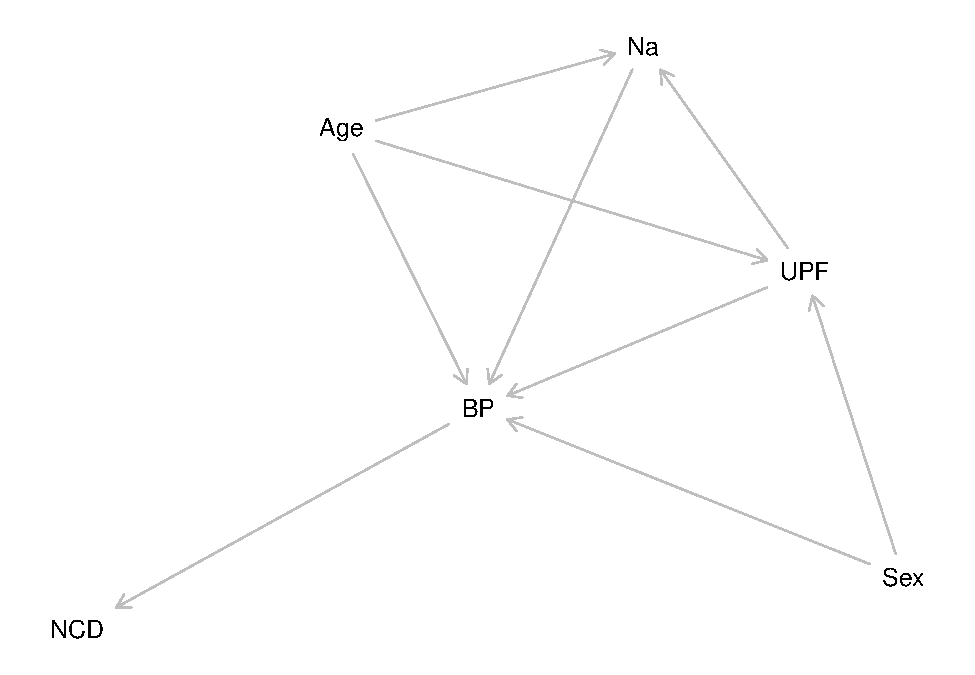
\includegraphics{methodandresults_files/figure-latex/fig-dag-1.pdf}
\caption{DAG of relationships explored by analysis}
\end{figure}

(\textbf{fig-dag?}) shows a possible arrangement of the relationships
between UPF, Na and BP highlighting the onward relationship to
non-contagious disease, and the underlying importance of age and sex.
This paper will seek to explore this complex web by pulling out strands
within it.

\hypertarget{public-health-impact}{%
\subsubsection{Public Health Impact}\label{public-health-impact}}

Public Health intends to reduce the burden of ill health across the
population. BP is an indicator of the health of the population, in that
it is a risk factor for a number of non-communicable diseases (NCD)
Francesco P. Cappuccio and Capewell (2015) .

Dietary approaches to improving public health are able to deliver
proportionate and universal interventions to populations to reduce the
incidence of NCD. These can be delivered up stream at the policy level.
This is effective and efficient and minimises cost.

Dietary approaches can also be used by individuals. This approach risks
the development of a culture of blame of individuals whose choices are
limited by systems outside of their control. The commercial and social
determinants of health play out a significant role in research, and
delivery of public health improvements around food Marmot (2010) .

\hypertarget{epistemology}{%
\subsubsection{Epistemology}\label{epistemology}}

The epistemological approach of this study is positivist. I use a
quantitative approach in a mechanistic and deterministic model. However,
I am aware that this model is an incomplete description of the whole of
reality. So that whilst I work within this positivist framework, I am
aware that the model is limited by the isolation which defines the
parameters of the study.

In particular I am aware that real world application to dietary change
requires interaction with social and economic factors. These factors are
often much better understood within critical realist and social
constructionist models. The commercial and social determinants of health
are both constructionist models which have a great deal of impact on the
reality of dietary effects on BP and on the availability of UPF and on
their nutritional constituents.

\hypertarget{positionality}{%
\subsubsection{Positionality}\label{positionality}}

In a positivist paradigm the observer is external to the model.
Acknowledging that there are constructivist aspects to this study allows
that the observer is closer to the model. My positionality is therefore
of interest to interpretation of the derived model, but also to
understand reasons for decisions about the approach to the data. I share
with Jafar Jafar (2018) an intention to lead in describing my
positionality in this quantitative study.

I am from a biomedical background, which brings an attachment to
positivist ideals. However, as a practising physician I am aware of the
interaction of any number of social factors on the health of
participants as Evans and Trotter Evans and Trotter (n.d.) discuss .
These impact on food `choices', which might be determined by social
expectations as much as by income, or geography. They also impact on
`hard' clinical measurements such as BP. This can be affected by
position and room temperature as well as by the relationship between the
observer and the participant.

This work is primarily to complete requirements for an MPH degree which
means that it is influenced by factors around health equity and classic
epidemiology as taught on the course. It is produced in collaboration
with a research group with a long established reputation in food
research in public health, which may steer the results in a conservative
direction.

Positivist `grand isolation' may reduce the influence of these factors,
but they remain as influences.

I accept that to proceed, whilst I need to be aware of the limitations
of the positivist approach and the necessity of making pragmatic
selections that there is some degree of validity to the resulting
dataset. Otherwise, analysis of it would be of no purpose.

\newpage

\hypertarget{literature-review}{%
\section{Literature Review}\label{literature-review}}

\hypertarget{introduction-1}{%
\subsection{Introduction}\label{introduction-1}}

This section will describe the search strategy and techniques used to
identify articles to make up the review. Then there will be a review of
separate sections of the literature, before developing a synthesis of
the literature at present and explanation on how it relates to the
research question.

\hypertarget{search-strategy}{%
\subsection{Search Strategy}\label{search-strategy}}

The search strategy has a core systematic approach but is augmented with
additional items from a range of sources. The success of the search is
that it identifies a wide variety of articles which help to outline and
augment the argument developed.

My search aims to identify most of the related articles. Starting with a
broad search strategy, the results are narrowed identifying those of
particular relevance, by reading abstracts and cross referencing with
other papers. Also, after discussion colleagues passed on further
relevant literature.

In addition, I identify papers from the bibliographies of identified
papers. Reviews and meta-analyses are good at presenting search
strategies and identifying high value studies.

These identify search terms not initially included. Despite limiting the
search to high blood pressure many of these searches consider broader
clinical endpoints, using metabolic syndrome, diabetes and
cerebrovascular and cardiovascular disease.

My search terms are included in the table below. They were searched
through a meta database which includes Medline, and Ovid and Scopus.
This meta database enables an ongoing search which is able to send
messages about new articles as they are published.

\begin{longtable}[]{@{}
  >{\raggedright\arraybackslash}p{(\columnwidth - 0\tabcolsep) * \real{1.0000}}@{}}
\toprule()
\begin{minipage}[b]{\linewidth}\raggedright
Search Terms Used
\end{minipage} \\
\midrule()
\endhead
``ultra-processed food'' OR ``ultra-processed foods'' OR
``ultraprocessed food'' OR ``ultraprocessed foods'' OR ``ultra-processed
product'' OR ``ultra-processed products'' OR ``ultra-processing'' OR
``food processing'' OR ``processed food'' OR ``processed foods'' OR
``NOVA'' OR ``NOVA system'' OR ``NOVA food classification'' OR ``NOVA
classification system'') AND (hypertension OR ``high blood pressure'' OR
``high blood pressures'' OR ``blood pressure'' OR ``systolic pressure''
OR ``diastolic pressure'' OR ``systolic blood pressure'' OR ``diastolic
blood pressure'') AND (adult OR adults OR aged OR ``middle aged'' OR
elderly OR ``older adult'' \\
\bottomrule()
\end{longtable}

Table 2.1: Table of search terms used

\hypertarget{search-results}{%
\subsection{Search results}\label{search-results}}

This search produced 1328 results the search allowed medical, public
health, nursing articles to be prioritised and engineering, chemical,
and technology articles to be deprioritised.

There were no time limits, language limits or availability limits in the
initial search. These 1328 were reduced down by reading titles and
abstracts to identify relevant articles.

Papers were excluded which related to technology including food
technology. They were also excluded if the primary purpose of the paper
was unrelated to dietary or nutritional causes of clinical outcomes.

\hypertarget{overview-of-literature}{%
\subsubsection{Overview of literature}\label{overview-of-literature}}

The literature has developed over some time. The results arrange
themselves therefore into several groups. Firstly there are those which
describe the development of the argument that salt relates to BP and so
to NCD. UPF is a recent phrase developed within the Nova framework which
was described in 2009 so the arguments around UPF and its relation to BP
and so NCD are more recent. This later group build on the earlier work,
but importantly they only superficially analyse the way that UPF and
salt interact.

In addition papers may be categorised as primary research, systematic
reviews with meta analysis, model analysis, and papers which use the
other categories to consider public health policy approaches.

\begin{itemize}
\tightlist
\item
  1 describe literature
\item
  2 synthesise literature
\item
  3 critique literature
\item
  4 explain role of study within context
\end{itemize}

\hypertarget{na-bp-ncd-and-public-health}{%
\subsection{Na, BP, NCD and Public
Health}\label{na-bp-ncd-and-public-health}}

\begin{figure}
\centering
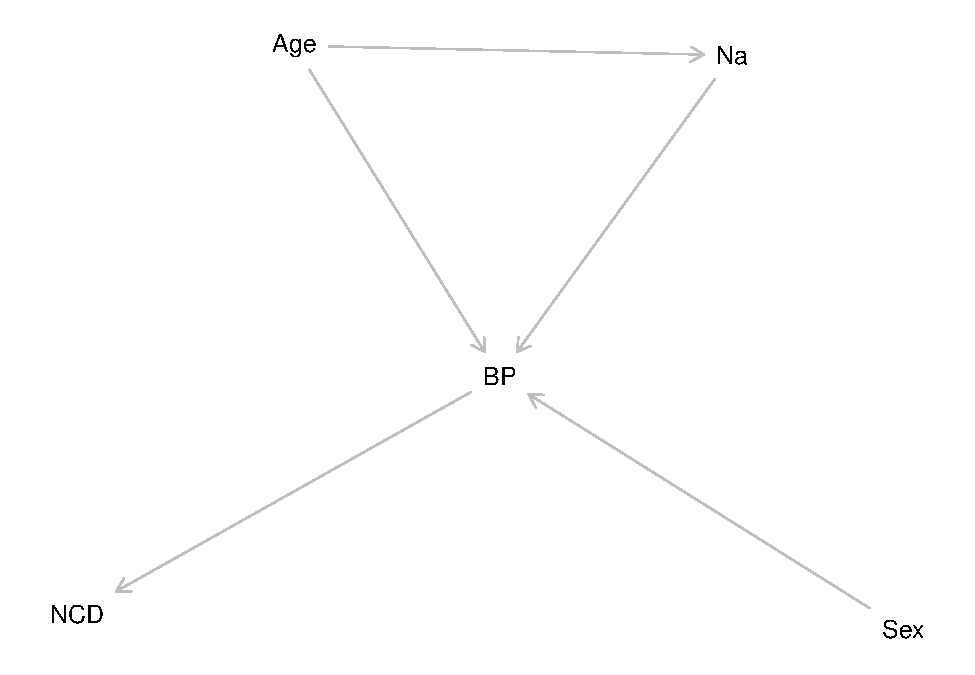
\includegraphics{methodandresults_files/figure-latex/fig-dagNa-1.pdf}
\caption{DAG of relationships between BP and Salt}
\end{figure}

Non-communicable disease is an increasing burden on public health.
Francesco P. Cappuccio and Capewell (2015) layout the charges against
salt most clearly. They identify comprehensively the connection between
changes in salt intake and changes in blood pressure and changes in
cardiovascular (CVD) and cerebrovascular diseases. They link the
nutritional effect of salt but they also identify the way this is
affected by social and commercial determinants of health. These are
branches from different epistemological backgrounds, nutrition from
positivism, and the social determinants from a more constructivist
approach.

Kannel (2009) , Kannel, Garrison, and Dannenberg (1993), and Mahmood et
al. (2014) describe how risk factor medicine came about. They describe
raised blood pressure as a `prominent member' of a group of risks in
cardiovascular disease. A disease which is the outcome of `multiple
forces'. Their description sees this as part of the march of progress in
understanding cardiovascular disease in particular, but also
non-communicable disease. Kannel identifies that cardiologists alone
cannot conquer cardiovascular disease. Since then BP has come to feature
more and more in NCD, following studies showing that reducing BP reduced
the risk of CVD . This placed Blood pressure detection, management, and
control at the centre of reducing CVD ( Bress et al. (2021) , Debon et
al. (2020) , Ettehad et al. (2016) , Pringle et al. (2003) , Roche and
Onyia (2018) ).

The causes of BP, as Kannel explains, are divided into secondary BP
where there is an identified pathological cause and `essential' or
idiopathic BP where no cause is identifiable. Contributors to and
partial causes of this essential BP have been sought, at individual and
societal levels, using medical and epidemiological approaches ( WHO
(n.d.) , {``Blood Pressure in the Normotensive Segment of the Population
Has Been Quite Stable.''} (n.d.) , {``Blood Pressure Test''} (2018) ).
Key factors are often separated into lifestyle causes ( Boutain (2001)
), and social determinants( Colombet et al. (2022) , Colombet et al.
(2019) , Ji and Cappuccio (2014) , Jones, Tong, and Monsivais (2018) ,
Leeuw and Simos (2017) , MacGregor, He, and Pombo-Rodrigues (2015) ).
Commerce also has a role to play in a causation model which embraces an
understanding of causation on a population scale.

Salt is a contributor to the physiology of BP. Its role in pathology is
less clear. There are increasing levels of intake. This is correlated
with increasing BP readings. Other nutrients have also been correlated.
The role of salt in normal and abnormal BP control is established (
Francesco P. Cappuccio and Capewell (2015) , {``Intersalt: An
International Study of Electrolyte Excretion and Blood Pressure. Results
for 24 Hour Urinary Sodium and Potassium Excretion. Intersalt
Cooperative Research Group.''} (1988) , (\textbf{elliot?}) , ). However
there remain areas of contention( Newman (2017) ). There may be
individuals with higher sensitivity to salt ( Elijovich (2016) ).
Understanding the best approaches to reducing salt is difficult.

Is it best to get individuals to reduce intake( {``Your Guide to
Lowering Your Blood Pressure with DASH''} (1998), {``Reports Outline
Obesity, Fitness and Wellness Findings from Federal University Vicosa
(Effects of Minimally and Ultra-processed Foods On Blood Pressure In
Brazilian Adults: a Two-year Follow Up of the Cume Project)''} (2023) ,
Vollmer et al. (2001) , Sacks et al. (2001) , Nilson et al. (2021) ), or
for all of the food industry to reduce salt levels( Francesco P.
Cappuccio et al. (2011) , He and MacGregor (2010) ).

\hypertarget{approach-to-change}{%
\subsubsection{Approach to change}\label{approach-to-change}}

Lifestyle factors are contented. Whilst individual choice is involved.
The range of choices available to individuals is limited by the nature
of their society. A misapplication of lifestyle results in blaming
individuals for the poor choices determined by their social and
commercial environment.

Instead of trying to change activity of millions of people can be more
effective to change laws and policies once ( Institute of Medicine et
al. (2010) , Laverty et al. (2019) , Millett et al. (2012) , Moreira et
al. (2015) , Institute of Medicine et al. (2013) ). These `upstream'
changes are relatively simple, and are much more effective though they
can also be reversed ( Francesco P. Cappuccio and Capewell (2015) ).
Opposition sometimes comes from industry.

Laverty et al. (2019) and MacGregor, He, and Pombo-Rodrigues (2015)
showed that an analytical model can effectively demonstrate the effects
of different policies on population health. They identify that reducing
the effectiveness of a policy on salt in food leads to changes in BP and
so on to NCD.

Campos-Nonato et al. (2022) identify the benefits of their strategy.
They discuss the range of nation level approaches to reducing salt
intake.

\begin{enumerate}
\def\labelenumi{\arabic{enumi}.}
\item
  Colombet et al. (2021)
\item
  Colombet Z, Simioni M, Drogue S, Lamani V, Perignon M, Martin-Prevel
  Y, et al. Demographic and socio-economic shifts partly explain the
  Martinican nutrition transition: an analysis of 10-year health and
  dietary changes (2003--2013) using decomposition models. Public health
  nutrition. 2021;24(18):6323--34.

  Iso et al. (1999)
\item
  Iso H, Shimamoto T, Yokota K, Ohki M, Sankai T, Kudo M, et
  al.~\[Changes in 24-hour urinary excretion of sodium and potassium in a community-based heath education program on salt reduction\].
  Nihon Koshu Eisei Zasshi. 1999 Oct;46(10):894--903.

  Jones, Tong, and Monsivais (2018)
\item
  Jones NR, Tong TY, Monsivais P. Meeting UK dietary recommendations is
  associated with higher estimated consumer food costs: an analysis
  using the National Diet and Nutrition Survey and consumer expenditure
  data, 2008--2012. Public Health Nutrition. 2018 Apr;21(5):948--56.

  (\textbf{healthy?})
\item
  Leeuw E de, Simos J, editors. Healthy cities: the theory, policy, and
  practice of value-based urban planning. New York, NY: Springer; 2017.
  515 p.
\item
  National Food Strategy, editor. National Food Strategy: part one.
  \[Internet\]. London: National Food Strategy,; 2020. Available from:
  \url{https://www.nationalfoodstrategy.org/partone/}
\end{enumerate}

\hypertarget{upf-and-bp}{%
\subsection{UPF and BP}\label{upf-and-bp}}

\hypertarget{dagupf}{%
\label{dagupf}}%
\begin{Shaded}
\begin{Highlighting}[]
\NormalTok{\{r dagupf, echo}\OtherTok{=}\ConstantTok{FALSE}\NormalTok{, message}\OtherTok{=}\ConstantTok{FALSE}\NormalTok{, warning}\OtherTok{=}\ConstantTok{FALSE}\NormalTok{\}}
\CommentTok{\#| label: fig{-}dag{-}upf}
\CommentTok{\#| fig{-}cap: "DAG of relationships of UPF"}

\NormalTok{bp3 }\OtherTok{\textless{}{-}} \FunctionTok{dagitty}\NormalTok{(}\StringTok{" dag \{}
\StringTok{             }
\StringTok{               Age {-}\textgreater{} BP}
\StringTok{               Sex {-}\textgreater{} BP}
\StringTok{               UPF {-}\textgreater{} BP}
\StringTok{              Age {-}\textgreater{} UPF}
\StringTok{               Sex {-}\textgreater{} UPF}
\StringTok{               BP {-}\textgreater{} NCD}
\StringTok{              }
\StringTok{\}"}\NormalTok{)}
\FunctionTok{plot}\NormalTok{(}\FunctionTok{graphLayout}\NormalTok{(bp3))}
\end{Highlighting}
\end{Shaded}

\hypertarget{upf}{%
\subsection{UPF}\label{upf}}

Nova classification looks at food beyond the nutrient level. It
incorporates ideas relating to `processing of food' But also includes
availability and intake which are all affected. Increasing Category four
or UPF is associated with increasing BP. Other approaches to food
classification try to address more than the nutritional content. There
is always conflict between commercial interests and restriction to the
freedom to exploitation

Food classification has traditionally concentrated on nutritional
analysis eg Nutriscore ( Cuj, Grabinsky, and Yates-Doerr (2021) , Dickie
et al. (2022), Romero Ferreiro, Lora Pablos, and Gómez de la Cámara
(2021) , A. et al. (2019) ). The social aspect of food has been studied
famously by Bourdieu ( Bourdieu and Bourdieu (2002), {``A
Bourdieu{'}dian Analysis for the Construction of an Education in Tea''}
(2021) ). The effect of the social and commercial nature of food is
partly accounted for in Monteiro's Nova classification. Dickie et al(
Dickie et al. (2023) , Dickie et al. (2022) ) tried to develop a system
which took this idea further, but struggled to build a model which was
any more effective.

Monteiro's initial explanation uses the concept of `processing' ( Carlos
A. Monteiro (2009) , Carlos A. Monteiro et al. (2016) , Carlos Augusto
Monteiro et al. (2010) , C. A. Monteiro et al. (2013) ). In a recent
debate Carlos A. Monteiro and Astrup (2022) and Astrup and Monteiro
(2022) discuss the concept of UPF and if it is valid or useful. This
idea separates foods into categories based on the amount of processing
that occurs before the food is consumed. Group one are foods which are
in a natural state, as plucked from the tree. Group two is foods which
are used in processes to modify group one foods. Group three initially
was all other foods, but was soon separated into minimally processed
foods, and group four the ultra-processed foods.

Explanations for the differential effect of these foods have developed
as quickly as new ultra-processed foods have been developed . Is it due
to nutritional content( Aceves-Martins et al. (2022) )? They are high in
salt and sugar on average. Is it due to effects on satiety, or changes
to appetite( Rauber et al. (2019) )? Do they taste better Bawajeeh et
al. (2021) ? Is it due to being easy to buy, and easy to eat( L. Wang et
al. (2021) )? Is it because they don't require time and effort in the
home to process? Is it because these processes are industrial? Is it
because these foods contain `chemicals' or new ingredients? These
explanations move from nutritional through into social and commercial.

All these critiques are possible because of the social element to the
classification. Colombet et al. (2022) identify that the intake of UPF
has an inequality dimension. Nutrition based classifications appear less
socially divisive due to scientific isolation. They still contain
elements of social factors. In particular, the way that foods are
analysed can change their reported nutritional content. Eg a `standard'
food may be compared to a `traditionally prepared' food. The first is
prepared in a factory with control of its nutrition, the second by a
home cook with limited access to nutrition modification technology.

Statements about the scheme often discuss the high salt and sugar
content. Papers discussing the effect on physiology, and pathology in
particular highlight these, but they do not back their statements with
analysis. They do not show that the sodium, and UPF together increase
the risk of CVD, or BP rise. This dissertation intends to address this
gap

Byker Shanks et al. (2022) show an approach between individual action
and changing laws. This approach would target those most at risk due to
negative social determinants. It does move into the realm of coercion of
those `making the wrong choices' into making better choices.

\hypertarget{increasing-upf}{%
\subsection{Increasing UPF}\label{increasing-upf}}

Many studies show the increasing role of UPF within the diet. Mertens,
Colizzi, and Peñalvo (2022) and Ni Mhurchu et al. (2011) show how UPF
are being eaten in ever greater quantities across Europe but especially
across the UK.

\hypertarget{upf-and-na}{%
\subsubsection{UPF and Na}\label{upf-and-na}}

Webster, Dunford, and Neal (2010) , Ni Mhurchu et al. (2011) contain
salt and

\hypertarget{upf-and-ill-health}{%
\subsubsection{UPF and Ill Health}\label{upf-and-ill-health}}

Oliveira et al. (2020) try to identify ill health in young people
associated with the increasing use of UPF.

\begin{enumerate}
\def\labelenumi{\arabic{enumi}.}
\item
  (\textbf{armendariz2022?})
\item
  Armendariz M, Pérez-Ferrer C, Basto-Abreu A, Lovasi GS, Bilal U,
  Barrientos-Gutiérrez T. Changes in the Retail Food Environment in
  Mexican Cities and Their Association with Blood Pressure Outcomes. Int
  J Environ Res Public Health. 2022 Jan 26;19(3):1353.

  D'avila and Kirsten (2017)
\item
  D'avila HF, Kirsten VR. Energy intake from ultra-processed foods among
  adolescents. Revista paulista de pediatria. 2017;35(1):54--60.

  Gupta, Khanal, and Khan (2021)
\item
  Gupta D, Khanal P, Khan M. Sustainability and ultra-processed foods:
  role of youth. Sustainability, agri, food and environmental research.
  2021;

  Hodge (2021)
\item
  Hodge A. In this issue: Ultra-processed food and health. Public health
  nutrition. 2021;24(11):3177--8.

  Muñoz-Lara et al. (2020)
\item
  Muñoz-Lara A, Moncada-Patiño J, Tovar-Vega A, Aguilar-Zavala H. THE
  CONSUMPTION OF ULTRA-PROCESSED FOODS, ANTHROPOMORPHIC MEASUREMENTS AND
  BLOOD CHEMISTRY IN MEXICAN SCHOOL-AGE CHILDREN. Annals of nutrition
  and metabolism. 2020;76:212-.

  Rauber et al. (2019)
\item
  Rauber F, Louzada ML da C, Steele EM, Rezende LFM de, Millett C,
  Monteiro CA, et al. Ultra-processed foods and excessive free sugar
  intake in the UK: a nationally representative cross-sectional study.
  BMJ Open. 2019 Oct 1;9(10):e027546.

  Rauber et al. (2020)
\item
  Rauber F, Steele EM, Louzada ML da C, Millett C, Monteiro CA, Levy RB.
  Ultra-processed food consumption and indicators of obesity in the
  United Kingdom population (2008-2016). Meyre D, editor. PLoS ONE. 2020
  May 1;15(5):e0232676.

  Southall (2022)
\item
  Southall JR. Ultra-processed food consumption linked to risk for
  colorectal cancer among men. HEM/ONC Today. 2022 Oct 25;23(14):13.

  Vargas-Meza et al. (2022)
\item
  Vargas-Meza J, Cervantes-Armenta MA, Campos-Nonato I, Nieto C,
  Marrón-Ponce JA, Barquera S, et al. Dietary sodium and potassium
  intake: Data from the mexican national health and nutrition survey
  2016. Nutrients. 2022;14(2):281-.

  (\textbf{wang2022?})
\item
  Wang L, Du M, Wang K, Khandpur N, Rossato SL, Drouin-Chartier JP, et
  al. Association of ultra-processed food consumption with colorectal
  cancer risk among men and women: results from three prospective US
  cohort studies. BMJ. 2022 Aug 31;378:e068921.

  L. Wang et al. (2021)
\item
  Wang L, Martínez Steele E, Du M, Pomeranz JL, O'Connor LE, Herrick KA,
  et al. Trends in Consumption of Ultraprocessed Foods Among US Youths
  Aged 2-19 Years, 1999-2018. JAMA. 2021 Aug 10;326(6):519--30.

  Weinstein et al. (2021)
\item
  Weinstein G, Vered S, Ivancovsky‐Wajcman D, Zelber‐Sagi S,
  Ravona‐Springer R, Heymann A, et al. Consumption of ultra‐processed
  food and cognitive decline among older adults with type‐2 diabetes.
  Alzheimer's \& dementia. 2021;17(S10).
\end{enumerate}

\hypertarget{section}{%
\subsection{}\label{section}}

Aceves-Martins et al. (2022)

\begin{enumerate}
\def\labelenumi{\arabic{enumi}.}
\item
  Aceves-Martins M, Link to external site this link will open in a new
  window, Bates RL, Link to external site this link will open in a new
  window, Craig LCA, Chalmers N, et al. Nutritional Quality,
  Environmental Impact and Cost of Ultra-Processed Foods: A UK
  Food-Based Analysis. International journal of environmental research
  and public health \[Internet\]. 2022 \[cited 2022 Oct 28\];19(6).
  Available from:
  \url{http://www.proquest.com/publiccontent/docview/2644005015?pq-origsite=primo}

  (\textbf{AguiarSarmentoRoberta2018EPaH?})
\item
  Aguiar Sarmento R, Peçanha Antonio J, Lamas de Miranda I, Bellicanta
  Nicoletto B, Carnevale de Almeida J. Eating patterns and health
  outcomes in patients with type 2 diabetes. Journal of the Endocrine
  Society. 2018;2(1):42--52.

  Barbosa et al. (2022)
\item
  Barbosa SS, Sousa LCM, de Oliveira Silva DF, Pimentel JB, Evangelista
  KCM de S, Lyra C de O, et al. A Systematic Review on
  Processed/Ultra-Processed Foods and Arterial Hypertension in Adults
  and Older People. Nutrients. 2022 Mar 13;14(6):1215.

  Colombet et al. (2019)
\item
  Colombet Z, Perignon M, Salanave B, Landais E, Martin-Prevel Y, Allès
  B, et al. Socioeconomic inequalities in metabolic syndrome in the
  French West Indies. BMC Public Health. 2019 Dec 3;19(1):1620.

  D'avila and Kirsten (2017)
\item
  D'Avila HF, Kirsten VR. CONSUMO ENERGÉTICO PROVENIENTE DE ALIMENTOS
  ULTRAPROCESSADOS POR ADOLESCENTES. Revista paulista de pediatria.
  2017;35(1):54--60.

  De Deus Mendonça et al. (2017)
\item
  De Deus Mendonça R, Souza Lopes AC, Pimenta AM, Gea A,
  Martinez-Gonzalez MA, Bes-Rastrollo M. Ultra-processed food
  consumption and the incidence of hypertension in a mediterranean
  cohort: The seguimiento universidad de navarra project. American
  journal of hypertension. 2017;30(4):358--66.

  Miranda, Rauber, and Levy (2021)
\item
  de Miranda RC, Rauber F, Levy RB. Impact of ultra-processed food
  consumption on metabolic health. Current opinion in lipidology.
  2021;32(1):24--37.

  Miranda, Rauber, and Levy (2021)
\item
  dos Santos FS, Dias M da S, Mintem GC, de Oliveira IO, Gigante DP.
  Food processing and cardiometabolic risk factors: a systematic review.
  Rev Saude Publica. 54:70.

  Gomez-Smith et al. (2018)
\item
  Gomez-Smith M, Janik R, Adams C, Lake EM, Thomason LAM, Jeffers MS, et
  al. Reduced cerebrovascular reactivity and increased resting cerebral
  perfusion in rats exposed to a cafeteria diet. Neuroscience.
  2018;371:166--77.

  Gonçalves et al. (2019)
\item
  Gonçalves VS, Duarte EC, Dutra ES, Barufaldi LA, Carvalho KM.
  Characteristics of the school food environment associated with
  hypertension and obesity in Brazilian adolescents: a multilevel
  analysis of the Study of Cardiovascular Risks in Adolescents (ERICA).
  Public health nutrition. 2019;22(14):2625--34.

  Goodman et al. (2020)
\item
  Goodman D, González-Rivas JP, Jaacks LM, Duran M, Marulanda MI, Ugel
  E, et al. Dietary intake and cardiometabolic risk factors among
  Venezuelan adults: a nationally representative analysis. BMC
  nutrition. 2020;6(1):61--61.

  Ivancovsky-Wajcman et al. (2021)
\item
  Ivancovsky‐Wajcman D, Fliss‐Isakov N, Webb M, Bentov I, Shibolet O,
  Kariv R, et al. Ultra‐processed food is associated with features of
  metabolic syndrome and non‐alcoholic fatty liver disease. Liver
  international. 2021;41(11):2635--45.

  Kityo and Lee (2022)
\item
  Kityo A, Lee SA. The intake of ultra-processed foods and prevalence of
  chronic kidney disease: The health examinees study. Nutrients.
  2022;14(17):3548-.

  Lee (2022)
\item
  Lee HY. Ultra-processed foods as a less-known risk factor in
  cardiovascular diseases. Korean circulation journal. 2022;52(1):71--3.

  Li and Shi (2022)
\item
  Li M, Link to external site this link will open in a new window, Shi
  Z, Link to external site this link will open in a new window.
  Association between Ultra-Processed Food Consumption and Diabetes in
  Chinese Adults-Results from the China Health and Nutrition Survey.
  Nutrients \[Internet\]. 2022 \[cited 2022 Nov 12\];14(20). Available
  from:
  \url{https://www.proquest.com/publiccontent/docview/2729520244?parentSessionId=8CgvVWDFcQEhyTTXC\%2B3zh7oBuY1vDlJi2c0\%2Fm7JmQZk\%3D\&pq-origsite=primo\&}

  Li and Shi (2021)
\item
  Li M, Shi Z. Ultra-processed food consumption associated with
  overweight/obesity among Chinese adults---Results from China health
  and nutrition survey 1997--2011. Nutrients. 2021;13(8):2796-.

  Li and Shi (2022)
\item
  Li M, Shi Z. Association between Ultra-Processed Food Consumption and
  Diabetes in Chinese Adults---Results from the China Health and
  Nutrition Survey. Nutrients. 2022 Jan;14(20):4241.

  Lima et al. (2011)
\item
  Lima R, Moreira L, Rossato S, Silva R, Fuchs S. P2-155 Consumption of
  ultra-processed food is associated with blood pressure in hypertensive
  individuals. Journal of epidemiology and community health (1979).
  2011;65(Suppl 1):A263--A263.

  (\textbf{Martinez-PerezCelia2021Uodf?})
\item
  Martínez Steele E, Juul F, Neri D, Rauber F, Monteiro CA. Dietary
  share of ultra-processed foods and metabolic syndrome in the US adult
  population. Preventive medicine. 2019;125:40--8.

  Oliveira et al. (2020)
\item
  Oliveira T, Ribeiro I, Jurema-Santos G, Nobre I, Santos R, Rodrigues
  C, et al. Can the consumption of ultra-processed food be associated
  with anthropometric indicators of obesity and blood pressure in
  children 7 to 10 years old? Foods. 2020;9(11):1567-.

  Rauber et al. (2019)
\item
  Rauber F, Louzada ML da C, Steele EM, Rezende LFM de, Millett C,
  Monteiro CA, et al. Ultra-processed foods and excessive free sugar
  intake in the UK: a nationally representative cross-sectional study.
  BMJ Open. 2019 Oct 1;9(10):e027546.

  Rauber et al. (2020)
\item
  Rauber F, Steele EM, Louzada ML da C, Millett C, Monteiro CA, Levy RB.
  Ultra-processed food consumption and indicators of obesity in the
  United Kingdom population (2008-2016). Meyre D, editor. PLoS ONE. 2020
  May 1;15(5):e0232676.

  Rezende-Alves et al. (2021)
\item
  Rezende-Alves K, Hermsdorff HHM, Miranda AE da S, Lopes ACS, Bressan
  J, Pimenta AM. Food processing and risk of hypertension: Cohort of
  universities of minas gerais, brazil (CUME project). Public health
  nutrition. 2021;24(13):4071--9.

  Santos et al. (2020)
\item
  Santos FSD, Dias M da S, Mintem GC, Oliveira IO de, Gigante DP. Food
  processing and cardiometabolic risk factors: a systematic review.
  Revista de saúde pública. 2020;54:70--70.

  (\textbf{scaranni?})
\item
  Scaranni P de O da S, Cardoso L de O, Chor D, Melo ECP, Matos SMA,
  Giatti L, et al. Ultra-processed foods, changes in blood pressure and
  incidence of hypertension: the Brazilian Longitudinal Study of Adult
  Health (ELSA-Brasil). Public health nutrition. 2021;24(11):3352--60.

  Schulze (2019)
\item
  Schulze K. UPF and cardiometabolic health \[Internet\]. University of
  Cambridge; 2019 \[cited 2023 Mar 2\]. Available from:
  \url{https://www.repository.cam.ac.uk/bitstream/handle/1810/306587/Kai\%20Schulze\%20Thesis\%202020_final.pdf?sequence=1\&isAllowed=y}

  (\textbf{shim2022?})
\item
  Shim SY, Kim HC, Shim JS. Consumption of ultra-processed food and
  blood pressure in korean adults. Korean circulation journal.
  2022;52(1):60--70.

  Smiljanec et al. (2020)
\item
  Smiljanec K, Mbakwe AU, Ramos-Gonzalez M, Mesbah C, Lennon SL.
  Associations of ultra-processed and unprocessed/minimally processed
  food consumption with peripheral and central hemodynamics, and
  arterial stiffness in young healthy adults. Nutrients.
  2020;12(11):1--19.

  (\textbf{suter2002?})
\item
  Suter PM, Sierro C, Vetter W. Nutritional Factors in the Control of
  Blood Pressure and Hypertension. Nutrition in Clinical Care.
  2002;5(1):9--19.

  Tavares et al. (2012)
\item
  Tavares LF, Fonseca SC, Garcia Rosa ML, Yokoo EM. Relationship between
  ultra-processed foods and metabolic syndrome in adolescents from a
  Brazilian Family Doctor Program. Public health nutrition.
  2012;15(1):82--7.

  Tzelefa et al. (2021)
\item
  Tzelefa V, Tsirimiagkou C, Argyris A, Moschonis G, Perogiannakis G,
  Yannakoulia M, et al. Associations of dietary patterns with blood
  pressure and markers of subclinical arterial damage in adults with
  risk factors for CVD. Public health nutrition. 2021;24(18):6075--84.

  Vilela et al. (2022)
\item
  Vilela S, Magalhães V, Severo M, Oliveira A, Torres D, Lopes C. Effect
  of the food processing degree on cardiometabolic health outcomes: A
  prospective approach in childhood. Clinical nutrition (Edinburgh,
  Scotland). 2022;41(10):2235--43.

  M. Wang et al. (2022)
\item
  Wang M, Du X, Huang W, Xu Y. Ultra-Processed Foods Consumption
  Increases the Risk of Hypertension in Adults: A Systematic Review and
  Meta-Analysis. American Journal of Hypertension. 2022 Oct
  1;35(10):892--901.
\end{enumerate}

\hypertarget{bp-upf-and-salt}{%
\subsection{BP UPF and Salt}\label{bp-upf-and-salt}}

What is not known is how UPF cause BP. Is it nutrient based? In which
case is this mediated by Salt? Is it other factors? This study looks
only at if Na is part of the causal pathway The thesis is that UPF is
more of a risk than the salt it contains

Many studies use quite carefully constructed categories to achieve
significant results.

Francesco P. Cappuccio and Capewell (2015)

\begin{enumerate}
\def\labelenumi{\arabic{enumi}.}
\item
  Cappuccio FP, Capewell S. Facts, Issues, and Controversies in Salt
  Reduction for the Prevention of Cardiovascular Disease. 2015;7(1):21.

  Elijovich (2016)
\item
  Elijovich F, Weinberger MH, Anderson CAM, Appel LJ, Bursztyn M, Cook
  NR, et al. Salt Sensitivity of Blood Pressure: A Scientific Statement
  From the American Heart Association. Hypertension. 2016
  Sep;68(3):e7--46.

  Elliott et al. (1996)
\item
  Elliott P, Stamler J, Nichols R, Dyer AR, Stamler R, Kesteloot H, et
  al. Intersalt revisited: further analyses of 24 hour sodium excretion
  and blood pressure within and across populations. BMJ. 1996 May
  18;312(7041):1249--53.

  He and MacGregor (2010)
\item
  He FJ, MacGregor GA. Reducing Population Salt Intake Worldwide: From
  Evidence to Implementation. Progress in Cardiovascular Diseases. 2010
  Mar 1;52(5):363--82.

  Nilson et al. (2021)
\item
  Nilson EAF, Spaniol AM, Santin R da C, Silva SA. Estratégias para
  redução do consumo de nutrientes críticos para a saúde: o caso do
  sódio. Cadernos de saúde pública. 2021;37(suppl 1).

  Sacks et al. (2001)
\item
  Sacks FM, Svetkey LP, Vollmer WM, Appel LJ, Bray GA, Harsha D, et al.
  Effects on Blood Pressure of Reduced Dietary Sodium and the Dietary
  Approaches to Stop Hypertension (DASH) Diet. New England Journal of
  Medicine. 2001 Jan 4;344(1):3--10.

  Vollmer et al. (2001)
\item
  Vollmer WM, Sacks FM, Ard J, Appel LJ, Bray GA, Simons-Morton DG, et
  al. Effects of Diet and Sodium Intake on Blood Pressure: Subgroup
  Analysis of the DASH-Sodium Trial. Ann Intern Med. 2001 Dec
  18;135(12):1019.

  {``Intersalt: An International Study of Electrolyte Excretion and
  Blood Pressure. Results for 24 Hour Urinary Sodium and Potassium
  Excretion. Intersalt Cooperative Research Group.''} (1988)
\item
  Intersalt: an international study of electrolyte excretion and blood
  pressure. Results for 24 hour urinary sodium and potassium excretion.
  Intersalt Cooperative Research Group. BMJ. 1988 Jul
  30;297(6644):319--28.

  {``Your Guide to Lowering Your Blood Pressure with DASH''} (1998)
\item
  Your Guide to Lowering Your Blood Pressure with DASH. US Department of
  Health and Human Services; 1998 p.~64.
\end{enumerate}

\newpage

\hypertarget{method}{%
\section{Method}\label{method}}

\hypertarget{introduction-2}{%
\subsection{Introduction}\label{introduction-2}}

This section takes the research question and explains how the data is
used to answer the question.

There will be a description of the study and data collection. Then a
section on governance and ethics in this project.

Data analysis starts with the relevant variables being identified and
extracted. Some data may need to be recalculated or to be processed to
make a more useable form. The population will be reviewed. Then there is
consideration of groups to be excluded.

There is a description of the data. The second analysis section compares
the data across the annual cohorts. The next analysis section involves
using linear regression to identify correlations. Firstly, between the
BP and each of the key variables. Then between other pairs of key
variables.

Multivariable regression models are then generated. These models are
examined to identify the relative importance of the different variables
in developing an optimal model and what these models tell us about the
relationship between our variables. A summary and conclusion will bring
all these together.

\hypertarget{research-question}{%
\subsection{Research Question}\label{research-question}}

What proportion of the association between blood pressure (SBP) and UPF
intake can be explained by the changes in salt intake in England between
2008 and 2019?

The question can be split into parts, What was intake of salt between
2008 and 2019? What was intake of UPF between 2008 and 2019? What was BP
between 2008 and 2019? Did each of these change over that time and how?
Did the changes in any one affect any other? What are the sizes of the
changes? Which element was most important in these changes?

All of these questions look for numbers as answers.

Answering the question starts with collecting a sample of participants.
Measurements are taken, and then collated. The collected numbers are
then compared in different ways to answer each part of the question.

\hypertarget{national-dietary-and-nutritional-survey}{%
\subsection{National Dietary and Nutritional
Survey}\label{national-dietary-and-nutritional-survey}}

This survey is a collaboration between government departments
responsible for health and for food production. They have engaged
academic partners to deliver reports on diet and nutrition across the
United Kingdom. The study is designed to be representative across the
whole area.

\hypertarget{study-design}{%
\subsubsection{Study design}\label{study-design}}

This is a rolling cohort study which each year selects a new cohort of
participants. The sample is approximately 1000 per year with 50\%
adults. The design has a random selection across postal units (psu).
This is stratified to ensure a representative sample across the four
nations and across regions within those countries. The sample is also
representative for age and sex.

Having taken up the study, participants complete a 4 day food diary, and
have an interview with a nurse which includes taking several
measurements. Weighting is given for each annual survey to enable
comparison across the years taking account for alterations in uptake and
response completion.

\hypertarget{ndns-dataset}{%
\subsubsection{NDNS Dataset}\label{ndns-dataset}}

The data from the NDNS study contains items about each individual,and
their household. It contains a table with each item of food as recorded
in their diary. There is a table with the overall intake of each of a
large range of nutrients for the whole period. This is calculated from
the diary using nutritional tables which are published as part of the
dataset. The dataset is available via the UK national Data service for
research purposes.

NDNS began before Monteiro's processing based classification, Nova , was
developed. There is no record of Nova food type in NDNS. This has been
calculated from the food descriptions. I have used a table from Rauber
et al Rauber et al. (2020) . for Nova values in NDNS.

\hypertarget{university-research-governance-and-ethical-review}{%
\subsubsection{University Research Governance and Ethical
Review}\label{university-research-governance-and-ethical-review}}

The research has been carried out under the University governance. A
proposal was discussed and agreed within the public health department.
The need for ethical review was considered using the university research
tool. The fact that the data is anonymised and there was no contact with
participants means that there is minimal risk of harm to research
participants. The initial proposal and a certificate from the ethics
department are in the appendices.

Other ethical issues include data custodianship ensuring that the the
rights of the owners of the data and of the participants are still
considered as part of the process of analysis and dissemination of the
research.

Issues around the power structures which lead to privilege one research
project or proposal over another are considered more in the
positionality section.

\hypertarget{data-processing}{%
\subsubsection{Data Processing}\label{data-processing}}

The storage of the data is in keeping with the research governance
agreements of the University and the Data set owners. The data is read
from its files using `r-studio' with the processing being carried out
using packages available from CRAN Team (2021) . I have used files which
had been amalgamated into four batches. These are 2008-2012, 2013-2014,
2015-2016, 2017-2019.

Once the data labels are made consistent across the batches, weighting
recalculation is done. This generates values which account for
differences in population balance across the annual cohorts. These
result from differences in compliance and uptake within and across the
years.

The years are amalgamated and the nature of the variables is specified.

\hypertarget{exclusions}{%
\subsubsection{Exclusions}\label{exclusions}}

The relationship between salt and systolic blood pressure may be
different in individuals with pathologically high BP. Those taking BP
controlling medications may have a different relationship to sodium and
UPF. These patients were excluded from the main analysis, however this
affected the sample size and skewed the male female ratio. Analysis was
done with exclusion and this produced results in line with those
presented, but of smaller magnitude. This additional analysis is not
presented here.

\hypertarget{description-of-the-data}{%
\subsection{Description of the data}\label{description-of-the-data}}

The data is summarised for the key continuous variables. The key
variables are systolic BP (omsysval), UPF intake (Epcnt\_4) and Sodium
intake (sodiummg). These variables are the ones which most relate to the
research question. (\textbf{tbl-keydata?}) shows the data which has been
balanced using the weightings provided by the NDNS research team.

There are a number of related variables in the dataset. These were
chosen for relevance, reliability and practicality. These variables are
ones which can also influence BP. They include Age, Sex, BMI, height and
weight. Age at completion of education (educfinh), and IMD are also
used.

The omsysval is a validated measurement with significant quality
assessment within the dataset. Raw systolic BP values are present in the
dataset but are made up of data with issues around quality. In
particular the systolic BP values are assessed for the effects of
exercise, temperature and ill health. The variable omsysval is a quality
assured mean value which is reliable across the dataset.

The sodium value is one calculated from intake based on food diaries and
standard food nutrient values. This only reflects standard foods and is
the result of assumptions about the content being consistent. Serum
sodium values are available for the early dataset, but not the later
one. There are also values for 24 urinary sodium which is probably a
better indicator of dietary sodium for parts of the dataset, but again
these are not found in both time periods. Though they were part of a
supplementary study.

The food diaries need processing to identify the UPF intake. Each
persons food diary entries are assessed against the Nova food
classification from Rauber. Then the weight and energy content of the
days food is calculated by Nova group. This is added to the intake for
the other 3 days and the total intake by Nova group established.

The percentage of the total intake of energy (Epcnt\_4) is then
calculated for each of the 4 Nova categories. Nova group 4 or UPF intake
is used for the study.

Mean values for the data are displayed with a comparison for weighted
values. The exposure variables are sodium intake (Sodiummg), and ultra
processed food intake (Epcnt\_4). The outcome variable, the mean
systolic blood pressure (omsysval).

\hypertarget{analysis-of-change-over-survey-years}{%
\subsubsection{Analysis of Change over Survey
Years}\label{analysis-of-change-over-survey-years}}

The second phase of analysis shows how the key variables have changed
over the survey years cohorts. This will show separately how the inputs
and outputs have changed.

These are not the same participants so matched analysis, or time series
analysis is not directly applicable.

Plots will be given to show the values in each of the available cohorts.

Other variables in the data are compared across to assess how the data
changes. Statistical significance of changes in the data are shown by
p.values with continuous data, and categorical data analysed using chi
squared tables.

\hypertarget{univariable-regression-of-key-variables}{%
\subsubsection{Univariable Regression of key
variables}\label{univariable-regression-of-key-variables}}

Analysis of the correlation between BP and sodium intake, and then BP
and UPF intake is done using linear regression. This will give an
indicator of the direction, and strength of any relationship between the
variables. There is also anova analysis to understand the statistical
significance of these results. Comparison is also made with Age, and
between each of the variables. This will show where significant
relationships are present.

\hypertarget{multiple-regression-on-systolic-bp-age-epcnt_4}{%
\subsubsection{Multiple Regression on Systolic BP (?age,
?Epcnt\_4)}\label{multiple-regression-on-systolic-bp-age-epcnt_4}}

Multivariable regression models are then developed to understand the
interactions between variables and to develop a mathematical model of
the relationship. The optimal model is one which best explains the
pattern of data, but which also makes practical sense for the wider
understanding of relationships. Assessment techniques try to understand
the importance of including particular variables, and the form in which
they are best included. Anova analysis here identifies how the addition
of different variables changes the significance of other variables. This
can suggest causative relationships. The resultant p.values help to
establish the statistical significance of the results.

\hypertarget{aic-and-sensitivty-anaylsis}{%
\subsubsection{AIC and sensitivty
Anaylsis}\label{aic-and-sensitivty-anaylsis}}

This section compares models side by side using assessment techniques to
identify the best way of describing the data. The `best' in part is
determined by the whether a model is needed to predict more data, or
just to understand the data available. Here it is about how best to
describe the relationship between Na, UPF, and BP.

\hypertarget{method-conclusion}{%
\subsection{Method Conclusion}\label{method-conclusion}}

This section has highlighted how the material for the study is brought
together and how the governance and ethics fit with the data collection,
processing and analysis to help us to derive the results which will be
presented in the next section.

\begin{verbatim}
\end{verbatim}

\newpage

\hypertarget{results}{%
\section{Results}\label{results}}

\hypertarget{results-introduction}{%
\subsection{Results Introduction}\label{results-introduction}}

Analysing the data from NDNS involves following the method. The
presented results are arranged to support explaining how the research
question is answered by the data.

The data used is described, explaining how it is structured. The data
analysis is then presented using tables and graphs to support the
argument. These most frequently present details of the statistical
significance of the proposed regression model.

The results section will be further interpreted in the discussion
section.

\hypertarget{description-of-the-data-1}{%
\subsection{Description of the Data}\label{description-of-the-data-1}}

This first table (\textbf{tbl-keydata?}) highlights the variables which
most relate to the research question from the years 2008-2019. These are
weighted values analysed using a software package called `survey' Lumley
(2004) .

The tables presented by NDNS have been amalgamated and new weighting
values calculated which enable comparison of data from separate tables.

There are several variables chosen. The number of participants in each
year, `N', is presented. The mean sodium intake in milligrams (Sodiummg)
is next. `Epcnt\_4' is the percent value of energy derived from Nova
category 4 foods, or UPF, out of the whole daily energy intake. The mean
Systolic BP value is one which has been validated within the NDNS study
it is given in mmHg.

These values are normally distributed continuous variables. The mean is
representative.

The numbers seem to be smaller towards the end of the series, for Sodium
intake, UPF intake (Epcnt\_4) and for systolic BP. Each cohort has been
adjusted to be comparable using weighting values given by the study
coordinators. However they are separate cohorts of separate participants
with no linear association between them. It can be seen that there are
lower values for all of the variables in the later groups.

\global\setlength{\Oldarrayrulewidth}{\arrayrulewidth}

\global\setlength{\Oldtabcolsep}{\tabcolsep}

\setlength{\tabcolsep}{0pt}

\renewcommand*{\arraystretch}{1.5}



\providecommand{\ascline}[3]{\noalign{\global\arrayrulewidth #1}\arrayrulecolor[HTML]{#2}\cline{#3}}

\begin{longtable}[c]{|p{2.86in}|p{1.27in}|p{1.27in}|p{1.27in}|p{1.27in}|p{1.27in}|p{1.27in}|p{1.27in}|p{1.27in}|p{1.27in}|p{1.37in}|p{1.37in}}



\ascline{1pt}{000000}{1-12}

\multicolumn{1}{>{\raggedright}m{\dimexpr 2.86in+0\tabcolsep}}{\textcolor[HTML]{000000}{\fontsize{11}{11}\selectfont{\textbf{Characteristic}}}} & \multicolumn{1}{>{\centering}m{\dimexpr 1.27in+0\tabcolsep}}{\textcolor[HTML]{000000}{\fontsize{11}{11}\selectfont{\textbf{1}}}\textcolor[HTML]{000000}{\fontsize{11}{11}\selectfont{,\ N\ =\ 1,459}}\textcolor[HTML]{000000}{\textsuperscript{\fontsize{11}{11}\selectfont{1}}}} & \multicolumn{1}{>{\centering}m{\dimexpr 1.27in+0\tabcolsep}}{\textcolor[HTML]{000000}{\fontsize{11}{11}\selectfont{\textbf{2}}}\textcolor[HTML]{000000}{\fontsize{11}{11}\selectfont{,\ N\ =\ 1,429}}\textcolor[HTML]{000000}{\textsuperscript{\fontsize{11}{11}\selectfont{1}}}} & \multicolumn{1}{>{\centering}m{\dimexpr 1.27in+0\tabcolsep}}{\textcolor[HTML]{000000}{\fontsize{11}{11}\selectfont{\textbf{3}}}\textcolor[HTML]{000000}{\fontsize{11}{11}\selectfont{,\ N\ =\ 1,372}}\textcolor[HTML]{000000}{\textsuperscript{\fontsize{11}{11}\selectfont{1}}}} & \multicolumn{1}{>{\centering}m{\dimexpr 1.27in+0\tabcolsep}}{\textcolor[HTML]{000000}{\fontsize{11}{11}\selectfont{\textbf{4}}}\textcolor[HTML]{000000}{\fontsize{11}{11}\selectfont{,\ N\ =\ 1,432}}\textcolor[HTML]{000000}{\textsuperscript{\fontsize{11}{11}\selectfont{1}}}} & \multicolumn{1}{>{\centering}m{\dimexpr 1.27in+0\tabcolsep}}{\textcolor[HTML]{000000}{\fontsize{11}{11}\selectfont{\textbf{5}}}\textcolor[HTML]{000000}{\fontsize{11}{11}\selectfont{,\ N\ =\ 1,485}}\textcolor[HTML]{000000}{\textsuperscript{\fontsize{11}{11}\selectfont{1}}}} & \multicolumn{1}{>{\centering}m{\dimexpr 1.27in+0\tabcolsep}}{\textcolor[HTML]{000000}{\fontsize{11}{11}\selectfont{\textbf{6}}}\textcolor[HTML]{000000}{\fontsize{11}{11}\selectfont{,\ N\ =\ 1,362}}\textcolor[HTML]{000000}{\textsuperscript{\fontsize{11}{11}\selectfont{1}}}} & \multicolumn{1}{>{\centering}m{\dimexpr 1.27in+0\tabcolsep}}{\textcolor[HTML]{000000}{\fontsize{11}{11}\selectfont{\textbf{7}}}\textcolor[HTML]{000000}{\fontsize{11}{11}\selectfont{,\ N\ =\ 1,442}}\textcolor[HTML]{000000}{\textsuperscript{\fontsize{11}{11}\selectfont{1}}}} & \multicolumn{1}{>{\centering}m{\dimexpr 1.27in+0\tabcolsep}}{\textcolor[HTML]{000000}{\fontsize{11}{11}\selectfont{\textbf{8}}}\textcolor[HTML]{000000}{\fontsize{11}{11}\selectfont{,\ N\ =\ 1,405}}\textcolor[HTML]{000000}{\textsuperscript{\fontsize{11}{11}\selectfont{1}}}} & \multicolumn{1}{>{\centering}m{\dimexpr 1.27in+0\tabcolsep}}{\textcolor[HTML]{000000}{\fontsize{11}{11}\selectfont{\textbf{9}}}\textcolor[HTML]{000000}{\fontsize{11}{11}\selectfont{,\ N\ =\ 1,444}}\textcolor[HTML]{000000}{\textsuperscript{\fontsize{11}{11}\selectfont{1}}}} & \multicolumn{1}{>{\centering}m{\dimexpr 1.37in+0\tabcolsep}}{\textcolor[HTML]{000000}{\fontsize{11}{11}\selectfont{\textbf{10}}}\textcolor[HTML]{000000}{\fontsize{11}{11}\selectfont{,\ N\ =\ 1,481}}\textcolor[HTML]{000000}{\textsuperscript{\fontsize{11}{11}\selectfont{1}}}} & \multicolumn{1}{>{\centering}m{\dimexpr 1.37in+0\tabcolsep}}{\textcolor[HTML]{000000}{\fontsize{11}{11}\selectfont{\textbf{11}}}\textcolor[HTML]{000000}{\fontsize{11}{11}\selectfont{,\ N\ =\ 1,345}}\textcolor[HTML]{000000}{\textsuperscript{\fontsize{11}{11}\selectfont{1}}}} \\

\ascline{1pt}{000000}{1-12}\endhead



\multicolumn{12}{>{\raggedright}m{\dimexpr 16.99in+22\tabcolsep}}{\textcolor[HTML]{000000}{\textsuperscript{\fontsize{11}{11}\selectfont{1}}}\textcolor[HTML]{000000}{\fontsize{11}{11}\selectfont{Mean\ (SD)}}} \\

\endfoot



\multicolumn{1}{>{\raggedright}p{\dimexpr 2.86in+0\tabcolsep}}{\textcolor[HTML]{000000}{\fontsize{11}{11}\selectfont{Sodium\ (mg)\ diet\ only}}} & \multicolumn{1}{>{\centering}p{\dimexpr 1.27in+0\tabcolsep}}{\textcolor[HTML]{000000}{\fontsize{11}{11}\selectfont{2,257\ (878)}}} & \multicolumn{1}{>{\centering}p{\dimexpr 1.27in+0\tabcolsep}}{\textcolor[HTML]{000000}{\fontsize{11}{11}\selectfont{2,208\ (827)}}} & \multicolumn{1}{>{\centering}p{\dimexpr 1.27in+0\tabcolsep}}{\textcolor[HTML]{000000}{\fontsize{11}{11}\selectfont{2,184\ (830)}}} & \multicolumn{1}{>{\centering}p{\dimexpr 1.27in+0\tabcolsep}}{\textcolor[HTML]{000000}{\fontsize{11}{11}\selectfont{2,077\ (799)}}} & \multicolumn{1}{>{\centering}p{\dimexpr 1.27in+0\tabcolsep}}{\textcolor[HTML]{000000}{\fontsize{11}{11}\selectfont{2,010\ (742)}}} & \multicolumn{1}{>{\centering}p{\dimexpr 1.27in+0\tabcolsep}}{\textcolor[HTML]{000000}{\fontsize{11}{11}\selectfont{1,988\ (765)}}} & \multicolumn{1}{>{\centering}p{\dimexpr 1.27in+0\tabcolsep}}{\textcolor[HTML]{000000}{\fontsize{11}{11}\selectfont{1,987\ (798)}}} & \multicolumn{1}{>{\centering}p{\dimexpr 1.27in+0\tabcolsep}}{\textcolor[HTML]{000000}{\fontsize{11}{11}\selectfont{1,945\ (822)}}} & \multicolumn{1}{>{\centering}p{\dimexpr 1.27in+0\tabcolsep}}{\textcolor[HTML]{000000}{\fontsize{11}{11}\selectfont{1,924\ (775)}}} & \multicolumn{1}{>{\centering}p{\dimexpr 1.37in+0\tabcolsep}}{\textcolor[HTML]{000000}{\fontsize{11}{11}\selectfont{1,892\ (724)}}} & \multicolumn{1}{>{\centering}p{\dimexpr 1.37in+0\tabcolsep}}{\textcolor[HTML]{000000}{\fontsize{11}{11}\selectfont{1,929\ (762)}}} \\





\multicolumn{1}{>{\raggedright}p{\dimexpr 2.86in+0\tabcolsep}}{\textcolor[HTML]{000000}{\fontsize{11}{11}\selectfont{Epcnt\_4}}} & \multicolumn{1}{>{\centering}p{\dimexpr 1.27in+0\tabcolsep}}{\textcolor[HTML]{000000}{\fontsize{11}{11}\selectfont{49\ (14)}}} & \multicolumn{1}{>{\centering}p{\dimexpr 1.27in+0\tabcolsep}}{\textcolor[HTML]{000000}{\fontsize{11}{11}\selectfont{50\ (15)}}} & \multicolumn{1}{>{\centering}p{\dimexpr 1.27in+0\tabcolsep}}{\textcolor[HTML]{000000}{\fontsize{11}{11}\selectfont{49\ (15)}}} & \multicolumn{1}{>{\centering}p{\dimexpr 1.27in+0\tabcolsep}}{\textcolor[HTML]{000000}{\fontsize{11}{11}\selectfont{49\ (15)}}} & \multicolumn{1}{>{\centering}p{\dimexpr 1.27in+0\tabcolsep}}{\textcolor[HTML]{000000}{\fontsize{11}{11}\selectfont{48\ (15)}}} & \multicolumn{1}{>{\centering}p{\dimexpr 1.27in+0\tabcolsep}}{\textcolor[HTML]{000000}{\fontsize{11}{11}\selectfont{50\ (16)}}} & \multicolumn{1}{>{\centering}p{\dimexpr 1.27in+0\tabcolsep}}{\textcolor[HTML]{000000}{\fontsize{11}{11}\selectfont{47\ (15)}}} & \multicolumn{1}{>{\centering}p{\dimexpr 1.27in+0\tabcolsep}}{\textcolor[HTML]{000000}{\fontsize{11}{11}\selectfont{45\ (16)}}} & \multicolumn{1}{>{\centering}p{\dimexpr 1.27in+0\tabcolsep}}{\textcolor[HTML]{000000}{\fontsize{11}{11}\selectfont{45\ (16)}}} & \multicolumn{1}{>{\centering}p{\dimexpr 1.37in+0\tabcolsep}}{\textcolor[HTML]{000000}{\fontsize{11}{11}\selectfont{45\ (15)}}} & \multicolumn{1}{>{\centering}p{\dimexpr 1.37in+0\tabcolsep}}{\textcolor[HTML]{000000}{\fontsize{11}{11}\selectfont{47\ (16)}}} \\





\multicolumn{1}{>{\raggedright}p{\dimexpr 2.86in+0\tabcolsep}}{\textcolor[HTML]{000000}{\fontsize{11}{11}\selectfont{(D)\ Omron\ valid\ mean\ systolic\ BP}}} & \multicolumn{1}{>{\centering}p{\dimexpr 1.27in+0\tabcolsep}}{\textcolor[HTML]{000000}{\fontsize{11}{11}\selectfont{125\ (19)}}} & \multicolumn{1}{>{\centering}p{\dimexpr 1.27in+0\tabcolsep}}{\textcolor[HTML]{000000}{\fontsize{11}{11}\selectfont{124\ (16)}}} & \multicolumn{1}{>{\centering}p{\dimexpr 1.27in+0\tabcolsep}}{\textcolor[HTML]{000000}{\fontsize{11}{11}\selectfont{124\ (18)}}} & \multicolumn{1}{>{\centering}p{\dimexpr 1.27in+0\tabcolsep}}{\textcolor[HTML]{000000}{\fontsize{11}{11}\selectfont{124\ (16)}}} & \multicolumn{1}{>{\centering}p{\dimexpr 1.27in+0\tabcolsep}}{\textcolor[HTML]{000000}{\fontsize{11}{11}\selectfont{122\ (17)}}} & \multicolumn{1}{>{\centering}p{\dimexpr 1.27in+0\tabcolsep}}{\textcolor[HTML]{000000}{\fontsize{11}{11}\selectfont{120\ (18)}}} & \multicolumn{1}{>{\centering}p{\dimexpr 1.27in+0\tabcolsep}}{\textcolor[HTML]{000000}{\fontsize{11}{11}\selectfont{124\ (19)}}} & \multicolumn{1}{>{\centering}p{\dimexpr 1.27in+0\tabcolsep}}{\textcolor[HTML]{000000}{\fontsize{11}{11}\selectfont{121\ (18)}}} & \multicolumn{1}{>{\centering}p{\dimexpr 1.27in+0\tabcolsep}}{\textcolor[HTML]{000000}{\fontsize{11}{11}\selectfont{121\ (17)}}} & \multicolumn{1}{>{\centering}p{\dimexpr 1.37in+0\tabcolsep}}{\textcolor[HTML]{000000}{\fontsize{11}{11}\selectfont{122\ (16)}}} & \multicolumn{1}{>{\centering}p{\dimexpr 1.37in+0\tabcolsep}}{\textcolor[HTML]{000000}{\fontsize{11}{11}\selectfont{0\ (0)}}} \\





\multicolumn{1}{>{\raggedright}p{\dimexpr 2.86in+0\tabcolsep}}{\textcolor[HTML]{000000}{\fontsize{11}{11}\selectfont{Unknown}}} & \multicolumn{1}{>{\centering}p{\dimexpr 1.27in+0\tabcolsep}}{\textcolor[HTML]{000000}{\fontsize{11}{11}\selectfont{609}}} & \multicolumn{1}{>{\centering}p{\dimexpr 1.27in+0\tabcolsep}}{\textcolor[HTML]{000000}{\fontsize{11}{11}\selectfont{639}}} & \multicolumn{1}{>{\centering}p{\dimexpr 1.27in+0\tabcolsep}}{\textcolor[HTML]{000000}{\fontsize{11}{11}\selectfont{604}}} & \multicolumn{1}{>{\centering}p{\dimexpr 1.27in+0\tabcolsep}}{\textcolor[HTML]{000000}{\fontsize{11}{11}\selectfont{654}}} & \multicolumn{1}{>{\centering}p{\dimexpr 1.27in+0\tabcolsep}}{\textcolor[HTML]{000000}{\fontsize{11}{11}\selectfont{551}}} & \multicolumn{1}{>{\centering}p{\dimexpr 1.27in+0\tabcolsep}}{\textcolor[HTML]{000000}{\fontsize{11}{11}\selectfont{574}}} & \multicolumn{1}{>{\centering}p{\dimexpr 1.27in+0\tabcolsep}}{\textcolor[HTML]{000000}{\fontsize{11}{11}\selectfont{588}}} & \multicolumn{1}{>{\centering}p{\dimexpr 1.27in+0\tabcolsep}}{\textcolor[HTML]{000000}{\fontsize{11}{11}\selectfont{541}}} & \multicolumn{1}{>{\centering}p{\dimexpr 1.27in+0\tabcolsep}}{\textcolor[HTML]{000000}{\fontsize{11}{11}\selectfont{562}}} & \multicolumn{1}{>{\centering}p{\dimexpr 1.37in+0\tabcolsep}}{\textcolor[HTML]{000000}{\fontsize{11}{11}\selectfont{529}}} & \multicolumn{1}{>{\centering}p{\dimexpr 1.37in+0\tabcolsep}}{\textcolor[HTML]{000000}{\fontsize{11}{11}\selectfont{1,345}}} \\

\ascline{1pt}{000000}{1-12}



\end{longtable}



\arrayrulecolor[HTML]{000000}

\global\setlength{\arrayrulewidth}{\Oldarrayrulewidth}

\global\setlength{\tabcolsep}{\Oldtabcolsep}

\renewcommand*{\arraystretch}{1}

\hypertarget{analysis-of-change-across-cohorts}{%
\subsection{Analysis of Change across
cohorts}\label{analysis-of-change-across-cohorts}}

These key variables are now compared between the cohorts.

(\textbf{fig-upf-and-survey-year?}) shows the energy from UPF in percent
(Epcnt\_4) against cohort number. This plot shows that the ranges
largely overlap. No visible difference is seen.

\begin{figure}
\centering
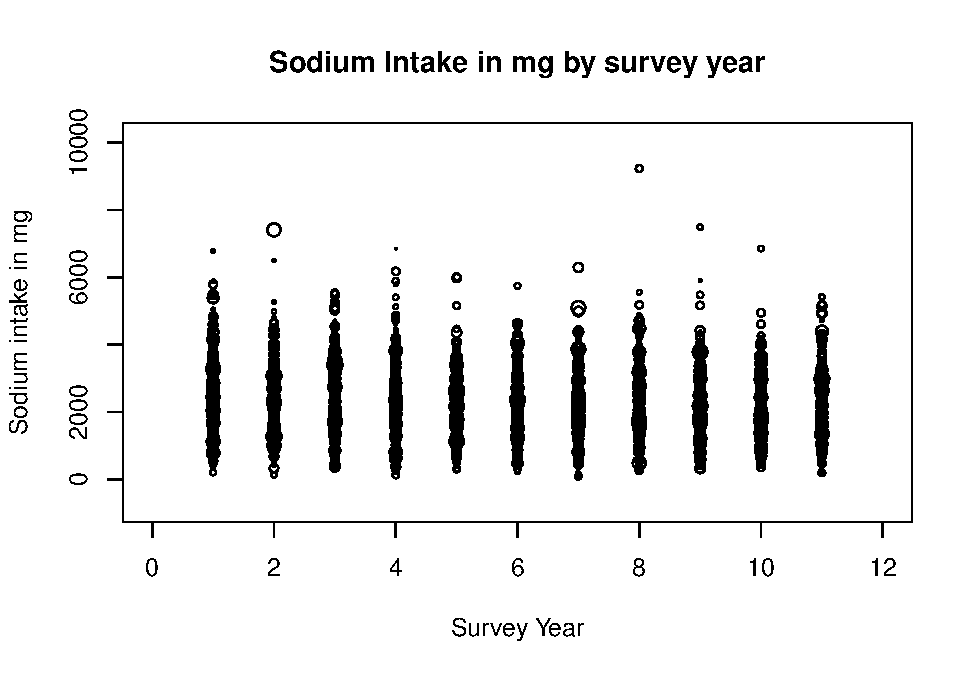
\includegraphics{methodandresults_files/figure-latex/fig-Na-and-survey-year-1.pdf}
\caption{Na-and-survey-year}
\end{figure}

The sodium intake (\textbf{fig-Na-and-survey-year?}), and the Systolic
BP (\textbf{fig-BP-and-survey-year?}) do not show an obvious change
across the cohorts.

\begin{verbatim}
## Warning: fonts used in `flextable` are ignored because the `pdflatex` engine is
## used and not `xelatex` or `lualatex`. You can avoid this warning by using the
## `set_flextable_defaults(fonts_ignore=TRUE)` command or use a compatible engine
## by defining `latex_engine: xelatex` in the YAML header of the R Markdown
## document.
\end{verbatim}

\global\setlength{\Oldarrayrulewidth}{\arrayrulewidth}

\global\setlength{\Oldtabcolsep}{\tabcolsep}

\setlength{\tabcolsep}{0pt}

\renewcommand*{\arraystretch}{1.5}



\providecommand{\ascline}[3]{\noalign{\global\arrayrulewidth #1}\arrayrulecolor[HTML]{#2}\cline{#3}}

\begin{longtable}[c]{|p{1.80in}|p{1.70in}|p{0.68in}|p{1.17in}|p{0.93in}}



\ascline{1pt}{000000}{1-5}

\multicolumn{1}{>{\raggedright}m{\dimexpr 1.8in+0\tabcolsep}}{\textcolor[HTML]{000000}{\fontsize{11}{11}\selectfont{\textbf{Group}}}} & \multicolumn{1}{>{\raggedright}m{\dimexpr 1.7in+0\tabcolsep}}{\textcolor[HTML]{000000}{\fontsize{11}{11}\selectfont{\textbf{Characteristic}}}} & \multicolumn{1}{>{\centering}m{\dimexpr 0.68in+0\tabcolsep}}{\textcolor[HTML]{000000}{\fontsize{11}{11}\selectfont{\textbf{Beta}}}} & \multicolumn{1}{>{\centering}m{\dimexpr 1.17in+0\tabcolsep}}{\textcolor[HTML]{000000}{\fontsize{11}{11}\selectfont{\textbf{95\%\ CI}}}\textcolor[HTML]{000000}{\textsuperscript{\fontsize{11}{11}\selectfont{1}}}} & \multicolumn{1}{>{\centering}m{\dimexpr 0.93in+0\tabcolsep}}{\textcolor[HTML]{000000}{\fontsize{11}{11}\selectfont{\textbf{p-value}}}} \\

\ascline{1pt}{000000}{1-5}\endhead



\multicolumn{5}{>{\raggedright}m{\dimexpr 6.27in+8\tabcolsep}}{\textcolor[HTML]{000000}{\textsuperscript{\fontsize{11}{11}\selectfont{1}}}\textcolor[HTML]{000000}{\fontsize{11}{11}\selectfont{CI\ =\ Confidence\ Interval}}} \\

\endfoot



\multicolumn{1}{>{\raggedright}p{\dimexpr 1.8in+0\tabcolsep}}{\textcolor[HTML]{000000}{\fontsize{11}{11}\selectfont{Sodium\ in\ mg}}} & \multicolumn{1}{>{\raggedright}p{\dimexpr 1.7in+0\tabcolsep}}{\textcolor[HTML]{000000}{\fontsize{11}{11}\selectfont{NDNS\ Survey\ year}}} & \multicolumn{1}{>{\centering}p{\dimexpr 0.68in+0\tabcolsep}}{\textcolor[HTML]{000000}{\fontsize{11}{11}\selectfont{-36}}} & \multicolumn{1}{>{\centering}p{\dimexpr 1.17in+0\tabcolsep}}{\textcolor[HTML]{000000}{\fontsize{11}{11}\selectfont{-43,\ -30}}} & \multicolumn{1}{>{\centering}p{\dimexpr 0.93in+0\tabcolsep}}{\textcolor[HTML]{000000}{\fontsize{11}{11}\selectfont{<0.001}}} \\





\multicolumn{1}{>{\raggedright}p{\dimexpr 1.8in+0\tabcolsep}}{\textcolor[HTML]{000000}{\fontsize{11}{11}\selectfont{Percent\ Energy\ UPF}}} & \multicolumn{1}{>{\raggedright}p{\dimexpr 1.7in+0\tabcolsep}}{\textcolor[HTML]{000000}{\fontsize{11}{11}\selectfont{NDNS\ Survey\ year}}} & \multicolumn{1}{>{\centering}p{\dimexpr 0.68in+0\tabcolsep}}{\textcolor[HTML]{000000}{\fontsize{11}{11}\selectfont{-0.41}}} & \multicolumn{1}{>{\centering}p{\dimexpr 1.17in+0\tabcolsep}}{\textcolor[HTML]{000000}{\fontsize{11}{11}\selectfont{-0.53,\ -0.29}}} & \multicolumn{1}{>{\centering}p{\dimexpr 0.93in+0\tabcolsep}}{\textcolor[HTML]{000000}{\fontsize{11}{11}\selectfont{<0.001}}} \\





\multicolumn{1}{>{\raggedright}p{\dimexpr 1.8in+0\tabcolsep}}{\textcolor[HTML]{000000}{\fontsize{11}{11}\selectfont{Systolic\ BP}}} & \multicolumn{1}{>{\raggedright}p{\dimexpr 1.7in+0\tabcolsep}}{\textcolor[HTML]{000000}{\fontsize{11}{11}\selectfont{NDNS\ Survey\ year}}} & \multicolumn{1}{>{\centering}p{\dimexpr 0.68in+0\tabcolsep}}{\textcolor[HTML]{000000}{\fontsize{11}{11}\selectfont{-0.37}}} & \multicolumn{1}{>{\centering}p{\dimexpr 1.17in+0\tabcolsep}}{\textcolor[HTML]{000000}{\fontsize{11}{11}\selectfont{-0.56,\ -0.19}}} & \multicolumn{1}{>{\centering}p{\dimexpr 0.93in+0\tabcolsep}}{\textcolor[HTML]{000000}{\fontsize{11}{11}\selectfont{<0.001}}} \\

\ascline{1pt}{000000}{1-5}



\end{longtable}



\arrayrulecolor[HTML]{000000}

\global\setlength{\arrayrulewidth}{\Oldarrayrulewidth}

\global\setlength{\tabcolsep}{\Oldtabcolsep}

\renewcommand*{\arraystretch}{1}

(\textbf{tbl-Key-Variables-by-SurveyYear?}) compares mean sodium, UPF
and systolic BP values across the individual cohorts. This uses cohort 1
as a comparator for the other cohorts. The differences and the beta
variable do not depend on there being a linear or ordinal arrangement
between the cohorts.

This shows that for sodium there is a beta of -36.2767894 with
confidence limits of -43, -30; For UPF beta is -0.4068208 and confidence
limits -0.53, -0.29; and for BP -0.3743859 and -0.56, -0.19. Each beta
value is negative which means that these values in each cohort is
largely below that of the first reference year. The confidence intervals
do not pass unity and so these results are statistically significant.

These corresponding negative beta values do not mean that there is a
correlation between these variables. This will be examined later.

\hypertarget{analysis-of-key-variables-by-sex}{%
\subsection{Analysis of key variables by
sex}\label{analysis-of-key-variables-by-sex}}

In each graph there is little difference apparent, though perhaps the
female plot is slightly lower.

\begin{verbatim}
## Warning: fonts used in `flextable` are ignored because the `pdflatex` engine is
## used and not `xelatex` or `lualatex`. You can avoid this warning by using the
## `set_flextable_defaults(fonts_ignore=TRUE)` command or use a compatible engine
## by defining `latex_engine: xelatex` in the YAML header of the R Markdown
## document.
\end{verbatim}

\global\setlength{\Oldarrayrulewidth}{\arrayrulewidth}

\global\setlength{\Oldtabcolsep}{\tabcolsep}

\setlength{\tabcolsep}{0pt}

\renewcommand*{\arraystretch}{1.5}



\providecommand{\ascline}[3]{\noalign{\global\arrayrulewidth #1}\arrayrulecolor[HTML]{#2}\cline{#3}}

\begin{longtable}[c]{|p{1.80in}|p{1.49in}|p{0.68in}|p{1.08in}|p{0.93in}}

\caption{Key\ Variables}\\

\ascline{1pt}{000000}{1-5}

\multicolumn{1}{>{\raggedright}m{\dimexpr 1.8in+0\tabcolsep}}{\textcolor[HTML]{000000}{\fontsize{11}{11}\selectfont{\textbf{Group}}}} & \multicolumn{1}{>{\raggedright}m{\dimexpr 1.49in+0\tabcolsep}}{\textcolor[HTML]{000000}{\fontsize{11}{11}\selectfont{\textbf{Characteristic}}}} & \multicolumn{1}{>{\centering}m{\dimexpr 0.68in+0\tabcolsep}}{\textcolor[HTML]{000000}{\fontsize{11}{11}\selectfont{\textbf{Beta}}}} & \multicolumn{1}{>{\centering}m{\dimexpr 1.08in+0\tabcolsep}}{\textcolor[HTML]{000000}{\fontsize{11}{11}\selectfont{\textbf{95\%\ CI}}}\textcolor[HTML]{000000}{\textsuperscript{\fontsize{11}{11}\selectfont{1}}}} & \multicolumn{1}{>{\centering}m{\dimexpr 0.93in+0\tabcolsep}}{\textcolor[HTML]{000000}{\fontsize{11}{11}\selectfont{\textbf{p-value}}}} \\

\ascline{1pt}{000000}{1-5}\endhead



\multicolumn{5}{>{\raggedright}m{\dimexpr 5.97in+8\tabcolsep}}{\textcolor[HTML]{000000}{\textsuperscript{\fontsize{11}{11}\selectfont{1}}}\textcolor[HTML]{000000}{\fontsize{11}{11}\selectfont{CI\ =\ Confidence\ Interval}}} \\

\endfoot



\multicolumn{1}{>{\raggedright}p{\dimexpr 1.8in+0\tabcolsep}}{\textcolor[HTML]{000000}{\fontsize{11}{11}\selectfont{Sodium\ in\ mg}}} & \multicolumn{1}{>{\raggedright}p{\dimexpr 1.49in+0\tabcolsep}}{\textcolor[HTML]{000000}{\fontsize{11}{11}\selectfont{Sex}}} & \multicolumn{1}{>{\centering}p{\dimexpr 0.68in+0\tabcolsep}}{\textcolor[HTML]{000000}{\fontsize{11}{11}\selectfont{}}} & \multicolumn{1}{>{\centering}p{\dimexpr 1.08in+0\tabcolsep}}{\textcolor[HTML]{000000}{\fontsize{11}{11}\selectfont{}}} & \multicolumn{1}{>{\centering}p{\dimexpr 0.93in+0\tabcolsep}}{\textcolor[HTML]{000000}{\fontsize{11}{11}\selectfont{}}} \\





\multicolumn{1}{>{\raggedright}p{\dimexpr 1.8in+0\tabcolsep}}{\textcolor[HTML]{000000}{\fontsize{11}{11}\selectfont{}}} & \multicolumn{1}{>{\raggedright}p{\dimexpr 1.49in+0\tabcolsep}}{\textcolor[HTML]{000000}{\fontsize{11}{11}\selectfont{Male}}} & \multicolumn{1}{>{\centering}p{\dimexpr 0.68in+0\tabcolsep}}{\textcolor[HTML]{000000}{\fontsize{11}{11}\selectfont{—}}} & \multicolumn{1}{>{\centering}p{\dimexpr 1.08in+0\tabcolsep}}{\textcolor[HTML]{000000}{\fontsize{11}{11}\selectfont{—}}} & \multicolumn{1}{>{\centering}p{\dimexpr 0.93in+0\tabcolsep}}{\textcolor[HTML]{000000}{\fontsize{11}{11}\selectfont{}}} \\





\multicolumn{1}{>{\raggedright}p{\dimexpr 1.8in+0\tabcolsep}}{\textcolor[HTML]{000000}{\fontsize{11}{11}\selectfont{}}} & \multicolumn{1}{>{\raggedright}p{\dimexpr 1.49in+0\tabcolsep}}{\textcolor[HTML]{000000}{\fontsize{11}{11}\selectfont{Female}}} & \multicolumn{1}{>{\centering}p{\dimexpr 0.68in+0\tabcolsep}}{\textcolor[HTML]{000000}{\fontsize{11}{11}\selectfont{-485}}} & \multicolumn{1}{>{\centering}p{\dimexpr 1.08in+0\tabcolsep}}{\textcolor[HTML]{000000}{\fontsize{11}{11}\selectfont{-523,\ -446}}} & \multicolumn{1}{>{\centering}p{\dimexpr 0.93in+0\tabcolsep}}{\textcolor[HTML]{000000}{\fontsize{11}{11}\selectfont{<0.001}}} \\





\multicolumn{1}{>{\raggedright}p{\dimexpr 1.8in+0\tabcolsep}}{\textcolor[HTML]{000000}{\fontsize{11}{11}\selectfont{Percent\ Energy\ UPF}}} & \multicolumn{1}{>{\raggedright}p{\dimexpr 1.49in+0\tabcolsep}}{\textcolor[HTML]{000000}{\fontsize{11}{11}\selectfont{Sex}}} & \multicolumn{1}{>{\centering}p{\dimexpr 0.68in+0\tabcolsep}}{\textcolor[HTML]{000000}{\fontsize{11}{11}\selectfont{}}} & \multicolumn{1}{>{\centering}p{\dimexpr 1.08in+0\tabcolsep}}{\textcolor[HTML]{000000}{\fontsize{11}{11}\selectfont{}}} & \multicolumn{1}{>{\centering}p{\dimexpr 0.93in+0\tabcolsep}}{\textcolor[HTML]{000000}{\fontsize{11}{11}\selectfont{}}} \\





\multicolumn{1}{>{\raggedright}p{\dimexpr 1.8in+0\tabcolsep}}{\textcolor[HTML]{000000}{\fontsize{11}{11}\selectfont{}}} & \multicolumn{1}{>{\raggedright}p{\dimexpr 1.49in+0\tabcolsep}}{\textcolor[HTML]{000000}{\fontsize{11}{11}\selectfont{Male}}} & \multicolumn{1}{>{\centering}p{\dimexpr 0.68in+0\tabcolsep}}{\textcolor[HTML]{000000}{\fontsize{11}{11}\selectfont{—}}} & \multicolumn{1}{>{\centering}p{\dimexpr 1.08in+0\tabcolsep}}{\textcolor[HTML]{000000}{\fontsize{11}{11}\selectfont{—}}} & \multicolumn{1}{>{\centering}p{\dimexpr 0.93in+0\tabcolsep}}{\textcolor[HTML]{000000}{\fontsize{11}{11}\selectfont{}}} \\





\multicolumn{1}{>{\raggedright}p{\dimexpr 1.8in+0\tabcolsep}}{\textcolor[HTML]{000000}{\fontsize{11}{11}\selectfont{}}} & \multicolumn{1}{>{\raggedright}p{\dimexpr 1.49in+0\tabcolsep}}{\textcolor[HTML]{000000}{\fontsize{11}{11}\selectfont{Female}}} & \multicolumn{1}{>{\centering}p{\dimexpr 0.68in+0\tabcolsep}}{\textcolor[HTML]{000000}{\fontsize{11}{11}\selectfont{-2.0}}} & \multicolumn{1}{>{\centering}p{\dimexpr 1.08in+0\tabcolsep}}{\textcolor[HTML]{000000}{\fontsize{11}{11}\selectfont{-2.7,\ -1.3}}} & \multicolumn{1}{>{\centering}p{\dimexpr 0.93in+0\tabcolsep}}{\textcolor[HTML]{000000}{\fontsize{11}{11}\selectfont{<0.001}}} \\





\multicolumn{1}{>{\raggedright}p{\dimexpr 1.8in+0\tabcolsep}}{\textcolor[HTML]{000000}{\fontsize{11}{11}\selectfont{Systolic\ BP}}} & \multicolumn{1}{>{\raggedright}p{\dimexpr 1.49in+0\tabcolsep}}{\textcolor[HTML]{000000}{\fontsize{11}{11}\selectfont{Sex}}} & \multicolumn{1}{>{\centering}p{\dimexpr 0.68in+0\tabcolsep}}{\textcolor[HTML]{000000}{\fontsize{11}{11}\selectfont{}}} & \multicolumn{1}{>{\centering}p{\dimexpr 1.08in+0\tabcolsep}}{\textcolor[HTML]{000000}{\fontsize{11}{11}\selectfont{}}} & \multicolumn{1}{>{\centering}p{\dimexpr 0.93in+0\tabcolsep}}{\textcolor[HTML]{000000}{\fontsize{11}{11}\selectfont{}}} \\





\multicolumn{1}{>{\raggedright}p{\dimexpr 1.8in+0\tabcolsep}}{\textcolor[HTML]{000000}{\fontsize{11}{11}\selectfont{}}} & \multicolumn{1}{>{\raggedright}p{\dimexpr 1.49in+0\tabcolsep}}{\textcolor[HTML]{000000}{\fontsize{11}{11}\selectfont{Male}}} & \multicolumn{1}{>{\centering}p{\dimexpr 0.68in+0\tabcolsep}}{\textcolor[HTML]{000000}{\fontsize{11}{11}\selectfont{—}}} & \multicolumn{1}{>{\centering}p{\dimexpr 1.08in+0\tabcolsep}}{\textcolor[HTML]{000000}{\fontsize{11}{11}\selectfont{—}}} & \multicolumn{1}{>{\centering}p{\dimexpr 0.93in+0\tabcolsep}}{\textcolor[HTML]{000000}{\fontsize{11}{11}\selectfont{}}} \\





\multicolumn{1}{>{\raggedright}p{\dimexpr 1.8in+0\tabcolsep}}{\textcolor[HTML]{000000}{\fontsize{11}{11}\selectfont{}}} & \multicolumn{1}{>{\raggedright}p{\dimexpr 1.49in+0\tabcolsep}}{\textcolor[HTML]{000000}{\fontsize{11}{11}\selectfont{Female}}} & \multicolumn{1}{>{\centering}p{\dimexpr 0.68in+0\tabcolsep}}{\textcolor[HTML]{000000}{\fontsize{11}{11}\selectfont{-5.5}}} & \multicolumn{1}{>{\centering}p{\dimexpr 1.08in+0\tabcolsep}}{\textcolor[HTML]{000000}{\fontsize{11}{11}\selectfont{-6.6,\ -4.5}}} & \multicolumn{1}{>{\centering}p{\dimexpr 0.93in+0\tabcolsep}}{\textcolor[HTML]{000000}{\fontsize{11}{11}\selectfont{<0.001}}} \\

\ascline{1pt}{000000}{1-5}



\end{longtable}



\arrayrulecolor[HTML]{000000}

\global\setlength{\arrayrulewidth}{\Oldarrayrulewidth}

\global\setlength{\tabcolsep}{\Oldtabcolsep}

\renewcommand*{\arraystretch}{1}

\hypertarget{analysis-of-key-variables-by-age}{%
\subsection{Analysis of Key Variables by
Age}\label{analysis-of-key-variables-by-age}}

\begin{figure}
\centering
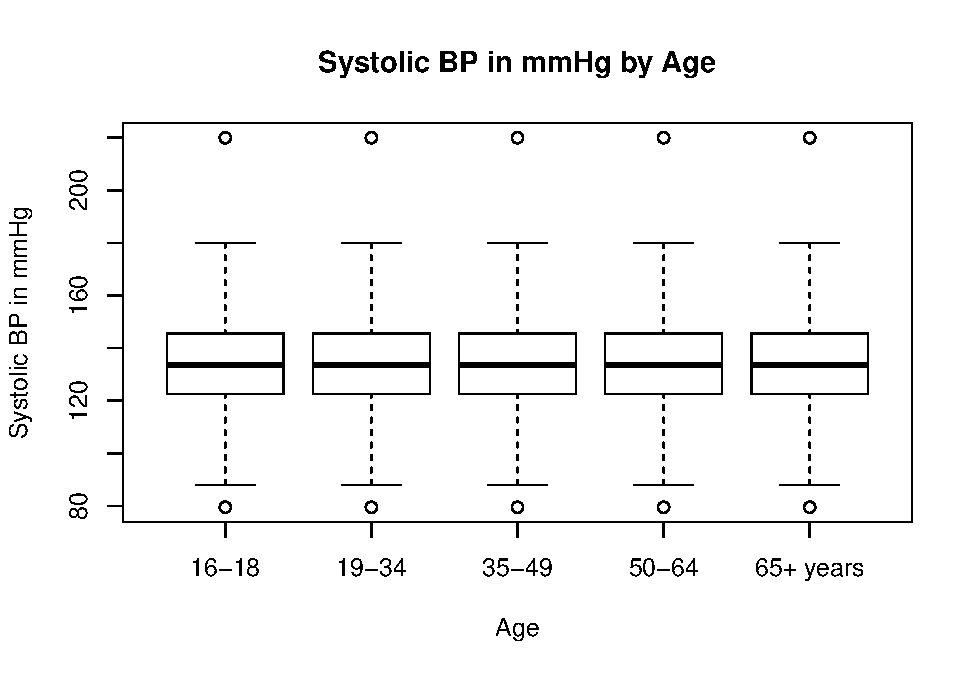
\includegraphics{methodandresults_files/figure-latex/fig-BP-age-Boxplots-1.pdf}
\caption{BP-age-Boxplots full population}
\end{figure}

\begin{verbatim}
## Warning: fonts used in `flextable` are ignored because the `pdflatex` engine is
## used and not `xelatex` or `lualatex`. You can avoid this warning by using the
## `set_flextable_defaults(fonts_ignore=TRUE)` command or use a compatible engine
## by defining `latex_engine: xelatex` in the YAML header of the R Markdown
## document.
\end{verbatim}

\global\setlength{\Oldarrayrulewidth}{\arrayrulewidth}

\global\setlength{\Oldtabcolsep}{\tabcolsep}

\setlength{\tabcolsep}{0pt}

\renewcommand*{\arraystretch}{1.5}



\providecommand{\ascline}[3]{\noalign{\global\arrayrulewidth #1}\arrayrulecolor[HTML]{#2}\cline{#3}}

\begin{longtable}[c]{|p{1.80in}|p{1.49in}|p{0.68in}|p{1.08in}|p{0.93in}}

\caption{Key\ Variables}\\

\ascline{1pt}{000000}{1-5}

\multicolumn{1}{>{\raggedright}m{\dimexpr 1.8in+0\tabcolsep}}{\textcolor[HTML]{000000}{\fontsize{11}{11}\selectfont{\textbf{Group}}}} & \multicolumn{1}{>{\raggedright}m{\dimexpr 1.49in+0\tabcolsep}}{\textcolor[HTML]{000000}{\fontsize{11}{11}\selectfont{\textbf{Characteristic}}}} & \multicolumn{1}{>{\centering}m{\dimexpr 0.68in+0\tabcolsep}}{\textcolor[HTML]{000000}{\fontsize{11}{11}\selectfont{\textbf{Beta}}}} & \multicolumn{1}{>{\centering}m{\dimexpr 1.08in+0\tabcolsep}}{\textcolor[HTML]{000000}{\fontsize{11}{11}\selectfont{\textbf{95\%\ CI}}}\textcolor[HTML]{000000}{\textsuperscript{\fontsize{11}{11}\selectfont{1}}}} & \multicolumn{1}{>{\centering}m{\dimexpr 0.93in+0\tabcolsep}}{\textcolor[HTML]{000000}{\fontsize{11}{11}\selectfont{\textbf{p-value}}}} \\

\ascline{1pt}{000000}{1-5}\endhead



\multicolumn{5}{>{\raggedright}m{\dimexpr 5.97in+8\tabcolsep}}{\textcolor[HTML]{000000}{\textsuperscript{\fontsize{11}{11}\selectfont{1}}}\textcolor[HTML]{000000}{\fontsize{11}{11}\selectfont{CI\ =\ Confidence\ Interval}}} \\

\endfoot



\multicolumn{1}{>{\raggedright}p{\dimexpr 1.8in+0\tabcolsep}}{\textcolor[HTML]{000000}{\fontsize{11}{11}\selectfont{Sodium\ in\ mg}}} & \multicolumn{1}{>{\raggedright}p{\dimexpr 1.49in+0\tabcolsep}}{\textcolor[HTML]{000000}{\fontsize{11}{11}\selectfont{agegad2}}} & \multicolumn{1}{>{\centering}p{\dimexpr 0.68in+0\tabcolsep}}{\textcolor[HTML]{000000}{\fontsize{11}{11}\selectfont{}}} & \multicolumn{1}{>{\centering}p{\dimexpr 1.08in+0\tabcolsep}}{\textcolor[HTML]{000000}{\fontsize{11}{11}\selectfont{}}} & \multicolumn{1}{>{\centering}p{\dimexpr 0.93in+0\tabcolsep}}{\textcolor[HTML]{000000}{\fontsize{11}{11}\selectfont{}}} \\





\multicolumn{1}{>{\raggedright}p{\dimexpr 1.8in+0\tabcolsep}}{\textcolor[HTML]{000000}{\fontsize{11}{11}\selectfont{}}} & \multicolumn{1}{>{\raggedright}p{\dimexpr 1.49in+0\tabcolsep}}{\textcolor[HTML]{000000}{\fontsize{11}{11}\selectfont{16-18}}} & \multicolumn{1}{>{\centering}p{\dimexpr 0.68in+0\tabcolsep}}{\textcolor[HTML]{000000}{\fontsize{11}{11}\selectfont{—}}} & \multicolumn{1}{>{\centering}p{\dimexpr 1.08in+0\tabcolsep}}{\textcolor[HTML]{000000}{\fontsize{11}{11}\selectfont{—}}} & \multicolumn{1}{>{\centering}p{\dimexpr 0.93in+0\tabcolsep}}{\textcolor[HTML]{000000}{\fontsize{11}{11}\selectfont{}}} \\





\multicolumn{1}{>{\raggedright}p{\dimexpr 1.8in+0\tabcolsep}}{\textcolor[HTML]{000000}{\fontsize{11}{11}\selectfont{}}} & \multicolumn{1}{>{\raggedright}p{\dimexpr 1.49in+0\tabcolsep}}{\textcolor[HTML]{000000}{\fontsize{11}{11}\selectfont{19-34}}} & \multicolumn{1}{>{\centering}p{\dimexpr 0.68in+0\tabcolsep}}{\textcolor[HTML]{000000}{\fontsize{11}{11}\selectfont{151}}} & \multicolumn{1}{>{\centering}p{\dimexpr 1.08in+0\tabcolsep}}{\textcolor[HTML]{000000}{\fontsize{11}{11}\selectfont{70,\ 232}}} & \multicolumn{1}{>{\centering}p{\dimexpr 0.93in+0\tabcolsep}}{\textcolor[HTML]{000000}{\fontsize{11}{11}\selectfont{<0.001}}} \\





\multicolumn{1}{>{\raggedright}p{\dimexpr 1.8in+0\tabcolsep}}{\textcolor[HTML]{000000}{\fontsize{11}{11}\selectfont{}}} & \multicolumn{1}{>{\raggedright}p{\dimexpr 1.49in+0\tabcolsep}}{\textcolor[HTML]{000000}{\fontsize{11}{11}\selectfont{35-49}}} & \multicolumn{1}{>{\centering}p{\dimexpr 0.68in+0\tabcolsep}}{\textcolor[HTML]{000000}{\fontsize{11}{11}\selectfont{21}}} & \multicolumn{1}{>{\centering}p{\dimexpr 1.08in+0\tabcolsep}}{\textcolor[HTML]{000000}{\fontsize{11}{11}\selectfont{-53,\ 96}}} & \multicolumn{1}{>{\centering}p{\dimexpr 0.93in+0\tabcolsep}}{\textcolor[HTML]{000000}{\fontsize{11}{11}\selectfont{0.6}}} \\





\multicolumn{1}{>{\raggedright}p{\dimexpr 1.8in+0\tabcolsep}}{\textcolor[HTML]{000000}{\fontsize{11}{11}\selectfont{}}} & \multicolumn{1}{>{\raggedright}p{\dimexpr 1.49in+0\tabcolsep}}{\textcolor[HTML]{000000}{\fontsize{11}{11}\selectfont{50-64}}} & \multicolumn{1}{>{\centering}p{\dimexpr 0.68in+0\tabcolsep}}{\textcolor[HTML]{000000}{\fontsize{11}{11}\selectfont{-110}}} & \multicolumn{1}{>{\centering}p{\dimexpr 1.08in+0\tabcolsep}}{\textcolor[HTML]{000000}{\fontsize{11}{11}\selectfont{-181,\ -39}}} & \multicolumn{1}{>{\centering}p{\dimexpr 0.93in+0\tabcolsep}}{\textcolor[HTML]{000000}{\fontsize{11}{11}\selectfont{0.002}}} \\





\multicolumn{1}{>{\raggedright}p{\dimexpr 1.8in+0\tabcolsep}}{\textcolor[HTML]{000000}{\fontsize{11}{11}\selectfont{}}} & \multicolumn{1}{>{\raggedright}p{\dimexpr 1.49in+0\tabcolsep}}{\textcolor[HTML]{000000}{\fontsize{11}{11}\selectfont{65+\ years}}} & \multicolumn{1}{>{\centering}p{\dimexpr 0.68in+0\tabcolsep}}{\textcolor[HTML]{000000}{\fontsize{11}{11}\selectfont{-263}}} & \multicolumn{1}{>{\centering}p{\dimexpr 1.08in+0\tabcolsep}}{\textcolor[HTML]{000000}{\fontsize{11}{11}\selectfont{-331,\ -195}}} & \multicolumn{1}{>{\centering}p{\dimexpr 0.93in+0\tabcolsep}}{\textcolor[HTML]{000000}{\fontsize{11}{11}\selectfont{<0.001}}} \\





\multicolumn{1}{>{\raggedright}p{\dimexpr 1.8in+0\tabcolsep}}{\textcolor[HTML]{000000}{\fontsize{11}{11}\selectfont{Percent\ Energy\ UPF}}} & \multicolumn{1}{>{\raggedright}p{\dimexpr 1.49in+0\tabcolsep}}{\textcolor[HTML]{000000}{\fontsize{11}{11}\selectfont{agegad2}}} & \multicolumn{1}{>{\centering}p{\dimexpr 0.68in+0\tabcolsep}}{\textcolor[HTML]{000000}{\fontsize{11}{11}\selectfont{}}} & \multicolumn{1}{>{\centering}p{\dimexpr 1.08in+0\tabcolsep}}{\textcolor[HTML]{000000}{\fontsize{11}{11}\selectfont{}}} & \multicolumn{1}{>{\centering}p{\dimexpr 0.93in+0\tabcolsep}}{\textcolor[HTML]{000000}{\fontsize{11}{11}\selectfont{}}} \\





\multicolumn{1}{>{\raggedright}p{\dimexpr 1.8in+0\tabcolsep}}{\textcolor[HTML]{000000}{\fontsize{11}{11}\selectfont{}}} & \multicolumn{1}{>{\raggedright}p{\dimexpr 1.49in+0\tabcolsep}}{\textcolor[HTML]{000000}{\fontsize{11}{11}\selectfont{16-18}}} & \multicolumn{1}{>{\centering}p{\dimexpr 0.68in+0\tabcolsep}}{\textcolor[HTML]{000000}{\fontsize{11}{11}\selectfont{—}}} & \multicolumn{1}{>{\centering}p{\dimexpr 1.08in+0\tabcolsep}}{\textcolor[HTML]{000000}{\fontsize{11}{11}\selectfont{—}}} & \multicolumn{1}{>{\centering}p{\dimexpr 0.93in+0\tabcolsep}}{\textcolor[HTML]{000000}{\fontsize{11}{11}\selectfont{}}} \\





\multicolumn{1}{>{\raggedright}p{\dimexpr 1.8in+0\tabcolsep}}{\textcolor[HTML]{000000}{\fontsize{11}{11}\selectfont{}}} & \multicolumn{1}{>{\raggedright}p{\dimexpr 1.49in+0\tabcolsep}}{\textcolor[HTML]{000000}{\fontsize{11}{11}\selectfont{19-34}}} & \multicolumn{1}{>{\centering}p{\dimexpr 0.68in+0\tabcolsep}}{\textcolor[HTML]{000000}{\fontsize{11}{11}\selectfont{-8.1}}} & \multicolumn{1}{>{\centering}p{\dimexpr 1.08in+0\tabcolsep}}{\textcolor[HTML]{000000}{\fontsize{11}{11}\selectfont{-9.6,\ -6.6}}} & \multicolumn{1}{>{\centering}p{\dimexpr 0.93in+0\tabcolsep}}{\textcolor[HTML]{000000}{\fontsize{11}{11}\selectfont{<0.001}}} \\





\multicolumn{1}{>{\raggedright}p{\dimexpr 1.8in+0\tabcolsep}}{\textcolor[HTML]{000000}{\fontsize{11}{11}\selectfont{}}} & \multicolumn{1}{>{\raggedright}p{\dimexpr 1.49in+0\tabcolsep}}{\textcolor[HTML]{000000}{\fontsize{11}{11}\selectfont{35-49}}} & \multicolumn{1}{>{\centering}p{\dimexpr 0.68in+0\tabcolsep}}{\textcolor[HTML]{000000}{\fontsize{11}{11}\selectfont{-13}}} & \multicolumn{1}{>{\centering}p{\dimexpr 1.08in+0\tabcolsep}}{\textcolor[HTML]{000000}{\fontsize{11}{11}\selectfont{-14,\ -12}}} & \multicolumn{1}{>{\centering}p{\dimexpr 0.93in+0\tabcolsep}}{\textcolor[HTML]{000000}{\fontsize{11}{11}\selectfont{<0.001}}} \\





\multicolumn{1}{>{\raggedright}p{\dimexpr 1.8in+0\tabcolsep}}{\textcolor[HTML]{000000}{\fontsize{11}{11}\selectfont{}}} & \multicolumn{1}{>{\raggedright}p{\dimexpr 1.49in+0\tabcolsep}}{\textcolor[HTML]{000000}{\fontsize{11}{11}\selectfont{50-64}}} & \multicolumn{1}{>{\centering}p{\dimexpr 0.68in+0\tabcolsep}}{\textcolor[HTML]{000000}{\fontsize{11}{11}\selectfont{-16}}} & \multicolumn{1}{>{\centering}p{\dimexpr 1.08in+0\tabcolsep}}{\textcolor[HTML]{000000}{\fontsize{11}{11}\selectfont{-18,\ -15}}} & \multicolumn{1}{>{\centering}p{\dimexpr 0.93in+0\tabcolsep}}{\textcolor[HTML]{000000}{\fontsize{11}{11}\selectfont{<0.001}}} \\





\multicolumn{1}{>{\raggedright}p{\dimexpr 1.8in+0\tabcolsep}}{\textcolor[HTML]{000000}{\fontsize{11}{11}\selectfont{}}} & \multicolumn{1}{>{\raggedright}p{\dimexpr 1.49in+0\tabcolsep}}{\textcolor[HTML]{000000}{\fontsize{11}{11}\selectfont{65+\ years}}} & \multicolumn{1}{>{\centering}p{\dimexpr 0.68in+0\tabcolsep}}{\textcolor[HTML]{000000}{\fontsize{11}{11}\selectfont{-15}}} & \multicolumn{1}{>{\centering}p{\dimexpr 1.08in+0\tabcolsep}}{\textcolor[HTML]{000000}{\fontsize{11}{11}\selectfont{-17,\ -14}}} & \multicolumn{1}{>{\centering}p{\dimexpr 0.93in+0\tabcolsep}}{\textcolor[HTML]{000000}{\fontsize{11}{11}\selectfont{<0.001}}} \\





\multicolumn{1}{>{\raggedright}p{\dimexpr 1.8in+0\tabcolsep}}{\textcolor[HTML]{000000}{\fontsize{11}{11}\selectfont{Systolic\ BP}}} & \multicolumn{1}{>{\raggedright}p{\dimexpr 1.49in+0\tabcolsep}}{\textcolor[HTML]{000000}{\fontsize{11}{11}\selectfont{agegad2}}} & \multicolumn{1}{>{\centering}p{\dimexpr 0.68in+0\tabcolsep}}{\textcolor[HTML]{000000}{\fontsize{11}{11}\selectfont{}}} & \multicolumn{1}{>{\centering}p{\dimexpr 1.08in+0\tabcolsep}}{\textcolor[HTML]{000000}{\fontsize{11}{11}\selectfont{}}} & \multicolumn{1}{>{\centering}p{\dimexpr 0.93in+0\tabcolsep}}{\textcolor[HTML]{000000}{\fontsize{11}{11}\selectfont{}}} \\





\multicolumn{1}{>{\raggedright}p{\dimexpr 1.8in+0\tabcolsep}}{\textcolor[HTML]{000000}{\fontsize{11}{11}\selectfont{}}} & \multicolumn{1}{>{\raggedright}p{\dimexpr 1.49in+0\tabcolsep}}{\textcolor[HTML]{000000}{\fontsize{11}{11}\selectfont{16-18}}} & \multicolumn{1}{>{\centering}p{\dimexpr 0.68in+0\tabcolsep}}{\textcolor[HTML]{000000}{\fontsize{11}{11}\selectfont{—}}} & \multicolumn{1}{>{\centering}p{\dimexpr 1.08in+0\tabcolsep}}{\textcolor[HTML]{000000}{\fontsize{11}{11}\selectfont{—}}} & \multicolumn{1}{>{\centering}p{\dimexpr 0.93in+0\tabcolsep}}{\textcolor[HTML]{000000}{\fontsize{11}{11}\selectfont{}}} \\





\multicolumn{1}{>{\raggedright}p{\dimexpr 1.8in+0\tabcolsep}}{\textcolor[HTML]{000000}{\fontsize{11}{11}\selectfont{}}} & \multicolumn{1}{>{\raggedright}p{\dimexpr 1.49in+0\tabcolsep}}{\textcolor[HTML]{000000}{\fontsize{11}{11}\selectfont{19-34}}} & \multicolumn{1}{>{\centering}p{\dimexpr 0.68in+0\tabcolsep}}{\textcolor[HTML]{000000}{\fontsize{11}{11}\selectfont{2.9}}} & \multicolumn{1}{>{\centering}p{\dimexpr 1.08in+0\tabcolsep}}{\textcolor[HTML]{000000}{\fontsize{11}{11}\selectfont{1.4,\ 4.4}}} & \multicolumn{1}{>{\centering}p{\dimexpr 0.93in+0\tabcolsep}}{\textcolor[HTML]{000000}{\fontsize{11}{11}\selectfont{<0.001}}} \\





\multicolumn{1}{>{\raggedright}p{\dimexpr 1.8in+0\tabcolsep}}{\textcolor[HTML]{000000}{\fontsize{11}{11}\selectfont{}}} & \multicolumn{1}{>{\raggedright}p{\dimexpr 1.49in+0\tabcolsep}}{\textcolor[HTML]{000000}{\fontsize{11}{11}\selectfont{35-49}}} & \multicolumn{1}{>{\centering}p{\dimexpr 0.68in+0\tabcolsep}}{\textcolor[HTML]{000000}{\fontsize{11}{11}\selectfont{6.7}}} & \multicolumn{1}{>{\centering}p{\dimexpr 1.08in+0\tabcolsep}}{\textcolor[HTML]{000000}{\fontsize{11}{11}\selectfont{5.2,\ 8.2}}} & \multicolumn{1}{>{\centering}p{\dimexpr 0.93in+0\tabcolsep}}{\textcolor[HTML]{000000}{\fontsize{11}{11}\selectfont{<0.001}}} \\





\multicolumn{1}{>{\raggedright}p{\dimexpr 1.8in+0\tabcolsep}}{\textcolor[HTML]{000000}{\fontsize{11}{11}\selectfont{}}} & \multicolumn{1}{>{\raggedright}p{\dimexpr 1.49in+0\tabcolsep}}{\textcolor[HTML]{000000}{\fontsize{11}{11}\selectfont{50-64}}} & \multicolumn{1}{>{\centering}p{\dimexpr 0.68in+0\tabcolsep}}{\textcolor[HTML]{000000}{\fontsize{11}{11}\selectfont{14}}} & \multicolumn{1}{>{\centering}p{\dimexpr 1.08in+0\tabcolsep}}{\textcolor[HTML]{000000}{\fontsize{11}{11}\selectfont{12,\ 16}}} & \multicolumn{1}{>{\centering}p{\dimexpr 0.93in+0\tabcolsep}}{\textcolor[HTML]{000000}{\fontsize{11}{11}\selectfont{<0.001}}} \\





\multicolumn{1}{>{\raggedright}p{\dimexpr 1.8in+0\tabcolsep}}{\textcolor[HTML]{000000}{\fontsize{11}{11}\selectfont{}}} & \multicolumn{1}{>{\raggedright}p{\dimexpr 1.49in+0\tabcolsep}}{\textcolor[HTML]{000000}{\fontsize{11}{11}\selectfont{65+\ years}}} & \multicolumn{1}{>{\centering}p{\dimexpr 0.68in+0\tabcolsep}}{\textcolor[HTML]{000000}{\fontsize{11}{11}\selectfont{20}}} & \multicolumn{1}{>{\centering}p{\dimexpr 1.08in+0\tabcolsep}}{\textcolor[HTML]{000000}{\fontsize{11}{11}\selectfont{18,\ 22}}} & \multicolumn{1}{>{\centering}p{\dimexpr 0.93in+0\tabcolsep}}{\textcolor[HTML]{000000}{\fontsize{11}{11}\selectfont{<0.001}}} \\

\ascline{1pt}{000000}{1-5}



\end{longtable}



\arrayrulecolor[HTML]{000000}

\global\setlength{\arrayrulewidth}{\Oldarrayrulewidth}

\global\setlength{\tabcolsep}{\Oldtabcolsep}

\renewcommand*{\arraystretch}{1}

(\textbf{tbl-Key-Variables-by-age?}) is interesting in that it shows
that whilst the BP goes up across the age categories, the UPF intake
decreases. The changes in sodium content are particularly interesting as
they show that the older age groups have much lower sodium intake, but
the highest sodium intake in in the second group, with the first and
third being statistically no different.

There is a difference in the age of finishing education.

These next box plots, (\textbf{fig-BP-Sex-Boxplots?}) ,
(\textbf{fig-Na-Sex-Boxplots?}) , (\textbf{fig-UPF-Sex-Boxplots?}) show
the difference between the sexes in the key variables.

\hypertarget{comparison-of-other-variables}{%
\subsection{Comparison of other
variables}\label{comparison-of-other-variables}}

How are variables distributed between the cohorts. The NDNS dataset was
weighted to keep many of these the same between datasets. Continuous
variables are assessed using linear regression and categorical variables
using chi squared tests to give p.values.

Age and Sex The age of the two datasets does not show a statistically
significant change table x.

This might be due to differences in the numbers of excluded
participants. In particular there may be more younger people and women
taking e.g.~bblockers in one group.

This table (\textbf{tbl-continuous-data?})) suggests that there is a
significant difference in the bmi of the cohorts.

\global\setlength{\Oldarrayrulewidth}{\arrayrulewidth}

\global\setlength{\Oldtabcolsep}{\tabcolsep}

\setlength{\tabcolsep}{0pt}

\renewcommand*{\arraystretch}{1.5}



\providecommand{\ascline}[3]{\noalign{\global\arrayrulewidth #1}\arrayrulecolor[HTML]{#2}\cline{#3}}

\begin{longtable}[c]{|p{0.81in}|p{1.70in}|p{0.68in}|p{1.17in}|p{0.93in}}

\caption{Continuous\ Variables\ by\ survey\ year}\\

\ascline{1pt}{000000}{1-5}

\multicolumn{1}{>{\raggedright}m{\dimexpr 0.81in+0\tabcolsep}}{\textcolor[HTML]{000000}{\fontsize{11}{11}\selectfont{\textbf{Group}}}} & \multicolumn{1}{>{\raggedright}m{\dimexpr 1.7in+0\tabcolsep}}{\textcolor[HTML]{000000}{\fontsize{11}{11}\selectfont{\textbf{Characteristic}}}} & \multicolumn{1}{>{\centering}m{\dimexpr 0.68in+0\tabcolsep}}{\textcolor[HTML]{000000}{\fontsize{11}{11}\selectfont{\textbf{Beta}}}} & \multicolumn{1}{>{\centering}m{\dimexpr 1.17in+0\tabcolsep}}{\textcolor[HTML]{000000}{\fontsize{11}{11}\selectfont{\textbf{95\%\ CI}}}\textcolor[HTML]{000000}{\textsuperscript{\fontsize{11}{11}\selectfont{1}}}} & \multicolumn{1}{>{\centering}m{\dimexpr 0.93in+0\tabcolsep}}{\textcolor[HTML]{000000}{\fontsize{11}{11}\selectfont{\textbf{p-value}}}} \\

\ascline{1pt}{000000}{1-5}\endhead



\multicolumn{5}{>{\raggedright}m{\dimexpr 5.29in+8\tabcolsep}}{\textcolor[HTML]{000000}{\textsuperscript{\fontsize{11}{11}\selectfont{1}}}\textcolor[HTML]{000000}{\fontsize{11}{11}\selectfont{CI\ =\ Confidence\ Interval}}} \\

\endfoot



\multicolumn{1}{>{\raggedright}p{\dimexpr 0.81in+0\tabcolsep}}{\textcolor[HTML]{000000}{\fontsize{11}{11}\selectfont{Age}}} & \multicolumn{1}{>{\raggedright}p{\dimexpr 1.7in+0\tabcolsep}}{\textcolor[HTML]{000000}{\fontsize{11}{11}\selectfont{NDNS\ Survey\ year}}} & \multicolumn{1}{>{\centering}p{\dimexpr 0.68in+0\tabcolsep}}{\textcolor[HTML]{000000}{\fontsize{11}{11}\selectfont{0.10}}} & \multicolumn{1}{>{\centering}p{\dimexpr 1.17in+0\tabcolsep}}{\textcolor[HTML]{000000}{\fontsize{11}{11}\selectfont{-0.06,\ 0.25}}} & \multicolumn{1}{>{\centering}p{\dimexpr 0.93in+0\tabcolsep}}{\textcolor[HTML]{000000}{\fontsize{11}{11}\selectfont{0.2}}} \\





\multicolumn{1}{>{\raggedright}p{\dimexpr 0.81in+0\tabcolsep}}{\textcolor[HTML]{000000}{\fontsize{11}{11}\selectfont{BMI}}} & \multicolumn{1}{>{\raggedright}p{\dimexpr 1.7in+0\tabcolsep}}{\textcolor[HTML]{000000}{\fontsize{11}{11}\selectfont{NDNS\ Survey\ year}}} & \multicolumn{1}{>{\centering}p{\dimexpr 0.68in+0\tabcolsep}}{\textcolor[HTML]{000000}{\fontsize{11}{11}\selectfont{-0.09}}} & \multicolumn{1}{>{\centering}p{\dimexpr 1.17in+0\tabcolsep}}{\textcolor[HTML]{000000}{\fontsize{11}{11}\selectfont{-0.13,\ -0.04}}} & \multicolumn{1}{>{\centering}p{\dimexpr 0.93in+0\tabcolsep}}{\textcolor[HTML]{000000}{\fontsize{11}{11}\selectfont{<0.001}}} \\

\ascline{1pt}{000000}{1-5}



\end{longtable}



\arrayrulecolor[HTML]{000000}

\global\setlength{\arrayrulewidth}{\Oldarrayrulewidth}

\global\setlength{\tabcolsep}{\Oldtabcolsep}

\renewcommand*{\arraystretch}{1}

There is a difference in the age of finishing education.

The differences in qimd, are not statistically significant.

These values identify a significant difference in the number of
vegetarians

\global\setlength{\Oldarrayrulewidth}{\arrayrulewidth}

\global\setlength{\Oldtabcolsep}{\tabcolsep}

\setlength{\tabcolsep}{0pt}

\renewcommand*{\arraystretch}{1.5}



\providecommand{\ascline}[3]{\noalign{\global\arrayrulewidth #1}\arrayrulecolor[HTML]{#2}\cline{#3}}

\begin{longtable}[c]{|p{1.12in}|p{0.90in}}

\caption{Categorical\ variables\ against\ Survey\ Year}\\

\ascline{1.5pt}{666666}{1-2}

\multicolumn{1}{>{\raggedright}b{\dimexpr 1.12in+0\tabcolsep}}{\textcolor[HTML]{000000}{\fontsize{11}{11}\selectfont{Variable}}} & \multicolumn{1}{>{\raggedleft}b{\dimexpr 0.9in+0\tabcolsep}}{\textcolor[HTML]{000000}{\fontsize{11}{11}\selectfont{p.value}}\textcolor[HTML]{000000}{\textsuperscript{\fontsize{11}{11}\selectfont{1}}}} \\

\ascline{1.5pt}{666666}{1-2}\endhead



\multicolumn{2}{>{\raggedright}m{\dimexpr 2.02in+2\tabcolsep}}{\textcolor[HTML]{000000}{\textsuperscript{\fontsize{11}{11}\selectfont{1}}}\textcolor[HTML]{000000}{\fontsize{11}{11}\selectfont{Chi\ Squared\ for\ categorical\ data}}} \\

\endfoot



\multicolumn{1}{>{\raggedright}m{\dimexpr 1.12in+0\tabcolsep}}{\textcolor[HTML]{000000}{\fontsize{11}{11}\selectfont{Sex}}} & \multicolumn{1}{>{\raggedleft}m{\dimexpr 0.9in+0\tabcolsep}}{\textcolor[HTML]{000000}{\fontsize{11}{11}\selectfont{0.5921}}} \\





\multicolumn{1}{>{\raggedright}m{\dimexpr 1.12in+0\tabcolsep}}{\textcolor[HTML]{000000}{\fontsize{11}{11}\selectfont{Education}}} & \multicolumn{1}{>{\raggedleft}m{\dimexpr 0.9in+0\tabcolsep}}{\textcolor[HTML]{000000}{\fontsize{11}{11}\selectfont{0.0000}}} \\





\multicolumn{1}{>{\raggedright}m{\dimexpr 1.12in+0\tabcolsep}}{\textcolor[HTML]{000000}{\fontsize{11}{11}\selectfont{IMD}}} & \multicolumn{1}{>{\raggedleft}m{\dimexpr 0.9in+0\tabcolsep}}{\textcolor[HTML]{000000}{\fontsize{11}{11}\selectfont{0.2208}}} \\





\multicolumn{1}{>{\raggedright}m{\dimexpr 1.12in+0\tabcolsep}}{\textcolor[HTML]{000000}{\fontsize{11}{11}\selectfont{Vegetarian}}} & \multicolumn{1}{>{\raggedleft}m{\dimexpr 0.9in+0\tabcolsep}}{\textcolor[HTML]{000000}{\fontsize{11}{11}\selectfont{0.0245}}} \\

\ascline{1.5pt}{666666}{1-2}



\end{longtable}



\arrayrulecolor[HTML]{000000}

\global\setlength{\arrayrulewidth}{\Oldarrayrulewidth}

\global\setlength{\tabcolsep}{\Oldtabcolsep}

\renewcommand*{\arraystretch}{1}

\hypertarget{regression-of-key-variables-on-systolic-bp}{%
\subsection{Regression of key variables on Systolic
BP}\label{regression-of-key-variables-on-systolic-bp}}

Simple linear regression equations look for the relationship between the
dependant variable, and the independent variable. For these I am looking
at the whole dataset first (\textbf{fig-Na-by-BP?})

\begin{figure}
\centering
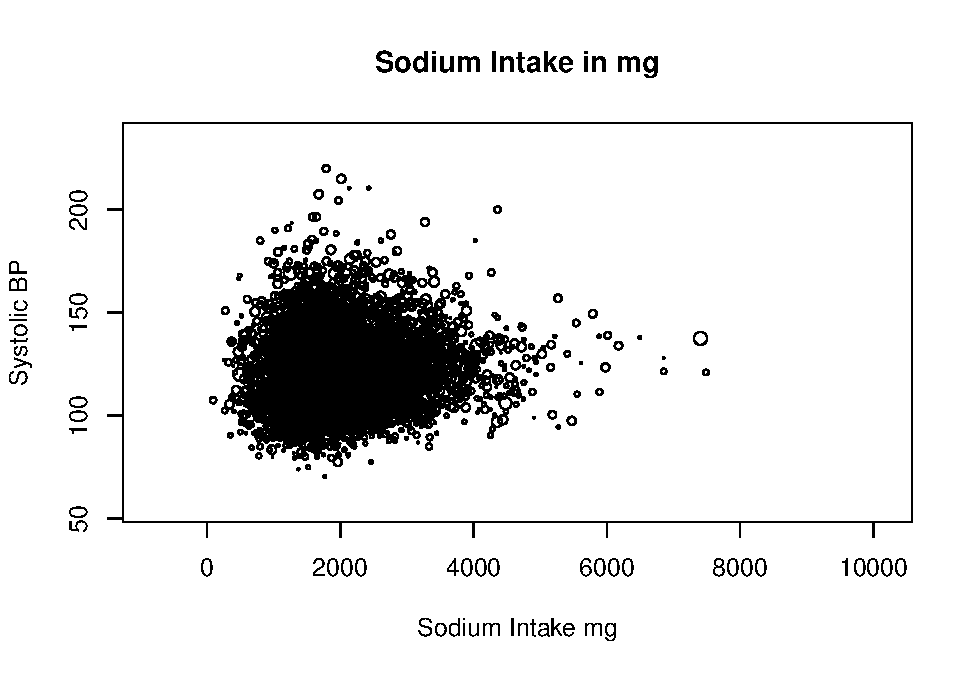
\includegraphics{methodandresults_files/figure-latex/fig-Na-by-BP-1.pdf}
\caption{Na-by-BP}
\end{figure}

Then (\textbf{fig-BP-and-UPF?})

and lastly (\textbf{fig-UPF-and-Na-plot?})

The regression models are examined for Sodium and UP against BP. These
use the populations where participants have been excluded. (analysis
including these makes no difference!!)

First, omsysval is compared to EnergykJ, then sodiummg.

\global\setlength{\Oldarrayrulewidth}{\arrayrulewidth}

\global\setlength{\Oldtabcolsep}{\tabcolsep}

\setlength{\tabcolsep}{0pt}

\renewcommand*{\arraystretch}{1.5}



\providecommand{\ascline}[3]{\noalign{\global\arrayrulewidth #1}\arrayrulecolor[HTML]{#2}\cline{#3}}

\begin{longtable}[c]{|p{0.92in}|p{1.99in}|p{0.68in}|p{1.17in}|p{0.93in}}

\caption{Univariable\ Regressions}\\

\ascline{1pt}{000000}{1-5}

\multicolumn{1}{>{\raggedright}m{\dimexpr 0.92in+0\tabcolsep}}{\textcolor[HTML]{000000}{\fontsize{11}{11}\selectfont{\textbf{Group}}}} & \multicolumn{1}{>{\raggedright}m{\dimexpr 1.99in+0\tabcolsep}}{\textcolor[HTML]{000000}{\fontsize{11}{11}\selectfont{\textbf{Characteristic}}}} & \multicolumn{1}{>{\centering}m{\dimexpr 0.68in+0\tabcolsep}}{\textcolor[HTML]{000000}{\fontsize{11}{11}\selectfont{\textbf{Beta}}}} & \multicolumn{1}{>{\centering}m{\dimexpr 1.17in+0\tabcolsep}}{\textcolor[HTML]{000000}{\fontsize{11}{11}\selectfont{\textbf{95\%\ CI}}}\textcolor[HTML]{000000}{\textsuperscript{\fontsize{11}{11}\selectfont{1}}}} & \multicolumn{1}{>{\centering}m{\dimexpr 0.93in+0\tabcolsep}}{\textcolor[HTML]{000000}{\fontsize{11}{11}\selectfont{\textbf{p-value}}}} \\

\ascline{1pt}{000000}{1-5}\endhead



\multicolumn{5}{>{\raggedright}m{\dimexpr 5.69in+8\tabcolsep}}{\textcolor[HTML]{000000}{\textsuperscript{\fontsize{11}{11}\selectfont{1}}}\textcolor[HTML]{000000}{\fontsize{11}{11}\selectfont{CI\ =\ Confidence\ Interval}}} \\

\endfoot



\multicolumn{1}{>{\raggedright}p{\dimexpr 0.92in+0\tabcolsep}}{\textcolor[HTML]{000000}{\fontsize{11}{11}\selectfont{BP/Na}}} & \multicolumn{1}{>{\raggedright}p{\dimexpr 1.99in+0\tabcolsep}}{\textcolor[HTML]{000000}{\fontsize{11}{11}\selectfont{Sodium\ (mg)\ diet\ only}}} & \multicolumn{1}{>{\centering}p{\dimexpr 0.68in+0\tabcolsep}}{\textcolor[HTML]{000000}{\fontsize{11}{11}\selectfont{0.00}}} & \multicolumn{1}{>{\centering}p{\dimexpr 1.17in+0\tabcolsep}}{\textcolor[HTML]{000000}{\fontsize{11}{11}\selectfont{0.00,\ 0.00}}} & \multicolumn{1}{>{\centering}p{\dimexpr 0.93in+0\tabcolsep}}{\textcolor[HTML]{000000}{\fontsize{11}{11}\selectfont{<0.001}}} \\





\multicolumn{1}{>{\raggedright}p{\dimexpr 0.92in+0\tabcolsep}}{\textcolor[HTML]{000000}{\fontsize{11}{11}\selectfont{UPF/Na}}} & \multicolumn{1}{>{\raggedright}p{\dimexpr 1.99in+0\tabcolsep}}{\textcolor[HTML]{000000}{\fontsize{11}{11}\selectfont{Sodium\ (mg)\ diet\ only}}} & \multicolumn{1}{>{\centering}p{\dimexpr 0.68in+0\tabcolsep}}{\textcolor[HTML]{000000}{\fontsize{11}{11}\selectfont{0.00}}} & \multicolumn{1}{>{\centering}p{\dimexpr 1.17in+0\tabcolsep}}{\textcolor[HTML]{000000}{\fontsize{11}{11}\selectfont{0.00,\ 0.00}}} & \multicolumn{1}{>{\centering}p{\dimexpr 0.93in+0\tabcolsep}}{\textcolor[HTML]{000000}{\fontsize{11}{11}\selectfont{<0.001}}} \\





\multicolumn{1}{>{\raggedright}p{\dimexpr 0.92in+0\tabcolsep}}{\textcolor[HTML]{000000}{\fontsize{11}{11}\selectfont{UPF/bp}}} & \multicolumn{1}{>{\raggedright}p{\dimexpr 1.99in+0\tabcolsep}}{\textcolor[HTML]{000000}{\fontsize{11}{11}\selectfont{Epcnt\_4}}} & \multicolumn{1}{>{\centering}p{\dimexpr 0.68in+0\tabcolsep}}{\textcolor[HTML]{000000}{\fontsize{11}{11}\selectfont{-0.21}}} & \multicolumn{1}{>{\centering}p{\dimexpr 1.17in+0\tabcolsep}}{\textcolor[HTML]{000000}{\fontsize{11}{11}\selectfont{-0.24,\ -0.17}}} & \multicolumn{1}{>{\centering}p{\dimexpr 0.93in+0\tabcolsep}}{\textcolor[HTML]{000000}{\fontsize{11}{11}\selectfont{<0.001}}} \\





\multicolumn{1}{>{\raggedright}p{\dimexpr 0.92in+0\tabcolsep}}{\textcolor[HTML]{000000}{\fontsize{11}{11}\selectfont{UPF/Age}}} & \multicolumn{1}{>{\raggedright}p{\dimexpr 1.99in+0\tabcolsep}}{\textcolor[HTML]{000000}{\fontsize{11}{11}\selectfont{Epcnt\_4}}} & \multicolumn{1}{>{\centering}p{\dimexpr 0.68in+0\tabcolsep}}{\textcolor[HTML]{000000}{\fontsize{11}{11}\selectfont{-0.46}}} & \multicolumn{1}{>{\centering}p{\dimexpr 1.17in+0\tabcolsep}}{\textcolor[HTML]{000000}{\fontsize{11}{11}\selectfont{-0.49,\ -0.44}}} & \multicolumn{1}{>{\centering}p{\dimexpr 0.93in+0\tabcolsep}}{\textcolor[HTML]{000000}{\fontsize{11}{11}\selectfont{<0.001}}} \\





\multicolumn{1}{>{\raggedright}p{\dimexpr 0.92in+0\tabcolsep}}{\textcolor[HTML]{000000}{\fontsize{11}{11}\selectfont{Age/BP}}} & \multicolumn{1}{>{\raggedright}p{\dimexpr 1.99in+0\tabcolsep}}{\textcolor[HTML]{000000}{\fontsize{11}{11}\selectfont{Age}}} & \multicolumn{1}{>{\centering}p{\dimexpr 0.68in+0\tabcolsep}}{\textcolor[HTML]{000000}{\fontsize{11}{11}\selectfont{0.43}}} & \multicolumn{1}{>{\centering}p{\dimexpr 1.17in+0\tabcolsep}}{\textcolor[HTML]{000000}{\fontsize{11}{11}\selectfont{0.40,\ 0.45}}} & \multicolumn{1}{>{\centering}p{\dimexpr 0.93in+0\tabcolsep}}{\textcolor[HTML]{000000}{\fontsize{11}{11}\selectfont{<0.001}}} \\





\multicolumn{1}{>{\raggedright}p{\dimexpr 0.92in+0\tabcolsep}}{\textcolor[HTML]{000000}{\fontsize{11}{11}\selectfont{Age/Na}}} & \multicolumn{1}{>{\raggedright}p{\dimexpr 1.99in+0\tabcolsep}}{\textcolor[HTML]{000000}{\fontsize{11}{11}\selectfont{Age}}} & \multicolumn{1}{>{\centering}p{\dimexpr 0.68in+0\tabcolsep}}{\textcolor[HTML]{000000}{\fontsize{11}{11}\selectfont{0.75}}} & \multicolumn{1}{>{\centering}p{\dimexpr 1.17in+0\tabcolsep}}{\textcolor[HTML]{000000}{\fontsize{11}{11}\selectfont{0.08,\ 1.4}}} & \multicolumn{1}{>{\centering}p{\dimexpr 0.93in+0\tabcolsep}}{\textcolor[HTML]{000000}{\fontsize{11}{11}\selectfont{0.028}}} \\

\ascline{1pt}{000000}{1-5}



\end{longtable}



\arrayrulecolor[HTML]{000000}

\global\setlength{\arrayrulewidth}{\Oldarrayrulewidth}

\global\setlength{\tabcolsep}{\Oldtabcolsep}

\renewcommand*{\arraystretch}{1}

\global\setlength{\Oldarrayrulewidth}{\arrayrulewidth}

\global\setlength{\Oldtabcolsep}{\tabcolsep}

\setlength{\tabcolsep}{0pt}

\renewcommand*{\arraystretch}{1.5}



\providecommand{\ascline}[3]{\noalign{\global\arrayrulewidth #1}\arrayrulecolor[HTML]{#2}\cline{#3}}

\begin{longtable}[c]{|p{0.93in}|p{1.49in}|p{0.68in}|p{1.22in}|p{0.93in}}

\caption{Univariable\ Regressions}\\

\ascline{1pt}{000000}{1-5}

\multicolumn{1}{>{\raggedright}m{\dimexpr 0.93in+0\tabcolsep}}{\textcolor[HTML]{000000}{\fontsize{11}{11}\selectfont{\textbf{Group}}}} & \multicolumn{1}{>{\raggedright}m{\dimexpr 1.49in+0\tabcolsep}}{\textcolor[HTML]{000000}{\fontsize{11}{11}\selectfont{\textbf{Characteristic}}}} & \multicolumn{1}{>{\centering}m{\dimexpr 0.68in+0\tabcolsep}}{\textcolor[HTML]{000000}{\fontsize{11}{11}\selectfont{\textbf{Beta}}}} & \multicolumn{1}{>{\centering}m{\dimexpr 1.22in+0\tabcolsep}}{\textcolor[HTML]{000000}{\fontsize{11}{11}\selectfont{\textbf{95\%\ CI}}}\textcolor[HTML]{000000}{\textsuperscript{\fontsize{11}{11}\selectfont{1}}}} & \multicolumn{1}{>{\centering}m{\dimexpr 0.93in+0\tabcolsep}}{\textcolor[HTML]{000000}{\fontsize{11}{11}\selectfont{\textbf{p-value}}}} \\

\ascline{1pt}{000000}{1-5}\endhead



\multicolumn{5}{>{\raggedright}m{\dimexpr 5.25in+8\tabcolsep}}{\textcolor[HTML]{000000}{\textsuperscript{\fontsize{11}{11}\selectfont{1}}}\textcolor[HTML]{000000}{\fontsize{11}{11}\selectfont{CI\ =\ Confidence\ Interval}}} \\

\endfoot



\multicolumn{1}{>{\raggedright}p{\dimexpr 0.93in+0\tabcolsep}}{\textcolor[HTML]{000000}{\fontsize{11}{11}\selectfont{BP/bmi}}} & \multicolumn{1}{>{\raggedright}p{\dimexpr 1.49in+0\tabcolsep}}{\textcolor[HTML]{000000}{\fontsize{11}{11}\selectfont{(D)\ Valid\ BMI}}} & \multicolumn{1}{>{\centering}p{\dimexpr 0.68in+0\tabcolsep}}{\textcolor[HTML]{000000}{\fontsize{11}{11}\selectfont{0.95}}} & \multicolumn{1}{>{\centering}p{\dimexpr 1.22in+0\tabcolsep}}{\textcolor[HTML]{000000}{\fontsize{11}{11}\selectfont{0.83,\ 1.1}}} & \multicolumn{1}{>{\centering}p{\dimexpr 0.93in+0\tabcolsep}}{\textcolor[HTML]{000000}{\fontsize{11}{11}\selectfont{<0.001}}} \\





\multicolumn{1}{>{\raggedright}p{\dimexpr 0.93in+0\tabcolsep}}{\textcolor[HTML]{000000}{\fontsize{11}{11}\selectfont{BP/Agg1}}} & \multicolumn{1}{>{\raggedright}p{\dimexpr 1.49in+0\tabcolsep}}{\textcolor[HTML]{000000}{\fontsize{11}{11}\selectfont{agegad1}}} & \multicolumn{1}{>{\centering}p{\dimexpr 0.68in+0\tabcolsep}}{\textcolor[HTML]{000000}{\fontsize{11}{11}\selectfont{}}} & \multicolumn{1}{>{\centering}p{\dimexpr 1.22in+0\tabcolsep}}{\textcolor[HTML]{000000}{\fontsize{11}{11}\selectfont{}}} & \multicolumn{1}{>{\centering}p{\dimexpr 0.93in+0\tabcolsep}}{\textcolor[HTML]{000000}{\fontsize{11}{11}\selectfont{}}} \\





\multicolumn{1}{>{\raggedright}p{\dimexpr 0.93in+0\tabcolsep}}{\textcolor[HTML]{000000}{\fontsize{11}{11}\selectfont{}}} & \multicolumn{1}{>{\raggedright}p{\dimexpr 1.49in+0\tabcolsep}}{\textcolor[HTML]{000000}{\fontsize{11}{11}\selectfont{16-24}}} & \multicolumn{1}{>{\centering}p{\dimexpr 0.68in+0\tabcolsep}}{\textcolor[HTML]{000000}{\fontsize{11}{11}\selectfont{—}}} & \multicolumn{1}{>{\centering}p{\dimexpr 1.22in+0\tabcolsep}}{\textcolor[HTML]{000000}{\fontsize{11}{11}\selectfont{—}}} & \multicolumn{1}{>{\centering}p{\dimexpr 0.93in+0\tabcolsep}}{\textcolor[HTML]{000000}{\fontsize{11}{11}\selectfont{}}} \\





\multicolumn{1}{>{\raggedright}p{\dimexpr 0.93in+0\tabcolsep}}{\textcolor[HTML]{000000}{\fontsize{11}{11}\selectfont{}}} & \multicolumn{1}{>{\raggedright}p{\dimexpr 1.49in+0\tabcolsep}}{\textcolor[HTML]{000000}{\fontsize{11}{11}\selectfont{25-49}}} & \multicolumn{1}{>{\centering}p{\dimexpr 0.68in+0\tabcolsep}}{\textcolor[HTML]{000000}{\fontsize{11}{11}\selectfont{3.5}}} & \multicolumn{1}{>{\centering}p{\dimexpr 1.22in+0\tabcolsep}}{\textcolor[HTML]{000000}{\fontsize{11}{11}\selectfont{2.0,\ 4.9}}} & \multicolumn{1}{>{\centering}p{\dimexpr 0.93in+0\tabcolsep}}{\textcolor[HTML]{000000}{\fontsize{11}{11}\selectfont{<0.001}}} \\





\multicolumn{1}{>{\raggedright}p{\dimexpr 0.93in+0\tabcolsep}}{\textcolor[HTML]{000000}{\fontsize{11}{11}\selectfont{}}} & \multicolumn{1}{>{\raggedright}p{\dimexpr 1.49in+0\tabcolsep}}{\textcolor[HTML]{000000}{\fontsize{11}{11}\selectfont{50-64}}} & \multicolumn{1}{>{\centering}p{\dimexpr 0.68in+0\tabcolsep}}{\textcolor[HTML]{000000}{\fontsize{11}{11}\selectfont{12}}} & \multicolumn{1}{>{\centering}p{\dimexpr 1.22in+0\tabcolsep}}{\textcolor[HTML]{000000}{\fontsize{11}{11}\selectfont{10,\ 14}}} & \multicolumn{1}{>{\centering}p{\dimexpr 0.93in+0\tabcolsep}}{\textcolor[HTML]{000000}{\fontsize{11}{11}\selectfont{<0.001}}} \\





\multicolumn{1}{>{\raggedright}p{\dimexpr 0.93in+0\tabcolsep}}{\textcolor[HTML]{000000}{\fontsize{11}{11}\selectfont{}}} & \multicolumn{1}{>{\raggedright}p{\dimexpr 1.49in+0\tabcolsep}}{\textcolor[HTML]{000000}{\fontsize{11}{11}\selectfont{65+\ years}}} & \multicolumn{1}{>{\centering}p{\dimexpr 0.68in+0\tabcolsep}}{\textcolor[HTML]{000000}{\fontsize{11}{11}\selectfont{18}}} & \multicolumn{1}{>{\centering}p{\dimexpr 1.22in+0\tabcolsep}}{\textcolor[HTML]{000000}{\fontsize{11}{11}\selectfont{16,\ 20}}} & \multicolumn{1}{>{\centering}p{\dimexpr 0.93in+0\tabcolsep}}{\textcolor[HTML]{000000}{\fontsize{11}{11}\selectfont{<0.001}}} \\





\multicolumn{1}{>{\raggedright}p{\dimexpr 0.93in+0\tabcolsep}}{\textcolor[HTML]{000000}{\fontsize{11}{11}\selectfont{BP/ed}}} & \multicolumn{1}{>{\raggedright}p{\dimexpr 1.49in+0\tabcolsep}}{\textcolor[HTML]{000000}{\fontsize{11}{11}\selectfont{educfinh}}} & \multicolumn{1}{>{\centering}p{\dimexpr 0.68in+0\tabcolsep}}{\textcolor[HTML]{000000}{\fontsize{11}{11}\selectfont{}}} & \multicolumn{1}{>{\centering}p{\dimexpr 1.22in+0\tabcolsep}}{\textcolor[HTML]{000000}{\fontsize{11}{11}\selectfont{}}} & \multicolumn{1}{>{\centering}p{\dimexpr 0.93in+0\tabcolsep}}{\textcolor[HTML]{000000}{\fontsize{11}{11}\selectfont{}}} \\





\multicolumn{1}{>{\raggedright}p{\dimexpr 0.93in+0\tabcolsep}}{\textcolor[HTML]{000000}{\fontsize{11}{11}\selectfont{}}} & \multicolumn{1}{>{\raggedright}p{\dimexpr 1.49in+0\tabcolsep}}{\textcolor[HTML]{000000}{\fontsize{11}{11}\selectfont{1}}} & \multicolumn{1}{>{\centering}p{\dimexpr 0.68in+0\tabcolsep}}{\textcolor[HTML]{000000}{\fontsize{11}{11}\selectfont{—}}} & \multicolumn{1}{>{\centering}p{\dimexpr 1.22in+0\tabcolsep}}{\textcolor[HTML]{000000}{\fontsize{11}{11}\selectfont{—}}} & \multicolumn{1}{>{\centering}p{\dimexpr 0.93in+0\tabcolsep}}{\textcolor[HTML]{000000}{\fontsize{11}{11}\selectfont{}}} \\





\multicolumn{1}{>{\raggedright}p{\dimexpr 0.93in+0\tabcolsep}}{\textcolor[HTML]{000000}{\fontsize{11}{11}\selectfont{}}} & \multicolumn{1}{>{\raggedright}p{\dimexpr 1.49in+0\tabcolsep}}{\textcolor[HTML]{000000}{\fontsize{11}{11}\selectfont{2}}} & \multicolumn{1}{>{\centering}p{\dimexpr 0.68in+0\tabcolsep}}{\textcolor[HTML]{000000}{\fontsize{11}{11}\selectfont{15}}} & \multicolumn{1}{>{\centering}p{\dimexpr 1.22in+0\tabcolsep}}{\textcolor[HTML]{000000}{\fontsize{11}{11}\selectfont{6.8,\ 23}}} & \multicolumn{1}{>{\centering}p{\dimexpr 0.93in+0\tabcolsep}}{\textcolor[HTML]{000000}{\fontsize{11}{11}\selectfont{<0.001}}} \\





\multicolumn{1}{>{\raggedright}p{\dimexpr 0.93in+0\tabcolsep}}{\textcolor[HTML]{000000}{\fontsize{11}{11}\selectfont{}}} & \multicolumn{1}{>{\raggedright}p{\dimexpr 1.49in+0\tabcolsep}}{\textcolor[HTML]{000000}{\fontsize{11}{11}\selectfont{3}}} & \multicolumn{1}{>{\centering}p{\dimexpr 0.68in+0\tabcolsep}}{\textcolor[HTML]{000000}{\fontsize{11}{11}\selectfont{21}}} & \multicolumn{1}{>{\centering}p{\dimexpr 1.22in+0\tabcolsep}}{\textcolor[HTML]{000000}{\fontsize{11}{11}\selectfont{17,\ 25}}} & \multicolumn{1}{>{\centering}p{\dimexpr 0.93in+0\tabcolsep}}{\textcolor[HTML]{000000}{\fontsize{11}{11}\selectfont{<0.001}}} \\





\multicolumn{1}{>{\raggedright}p{\dimexpr 0.93in+0\tabcolsep}}{\textcolor[HTML]{000000}{\fontsize{11}{11}\selectfont{}}} & \multicolumn{1}{>{\raggedright}p{\dimexpr 1.49in+0\tabcolsep}}{\textcolor[HTML]{000000}{\fontsize{11}{11}\selectfont{4}}} & \multicolumn{1}{>{\centering}p{\dimexpr 0.68in+0\tabcolsep}}{\textcolor[HTML]{000000}{\fontsize{11}{11}\selectfont{16}}} & \multicolumn{1}{>{\centering}p{\dimexpr 1.22in+0\tabcolsep}}{\textcolor[HTML]{000000}{\fontsize{11}{11}\selectfont{14,\ 19}}} & \multicolumn{1}{>{\centering}p{\dimexpr 0.93in+0\tabcolsep}}{\textcolor[HTML]{000000}{\fontsize{11}{11}\selectfont{<0.001}}} \\





\multicolumn{1}{>{\raggedright}p{\dimexpr 0.93in+0\tabcolsep}}{\textcolor[HTML]{000000}{\fontsize{11}{11}\selectfont{}}} & \multicolumn{1}{>{\raggedright}p{\dimexpr 1.49in+0\tabcolsep}}{\textcolor[HTML]{000000}{\fontsize{11}{11}\selectfont{5}}} & \multicolumn{1}{>{\centering}p{\dimexpr 0.68in+0\tabcolsep}}{\textcolor[HTML]{000000}{\fontsize{11}{11}\selectfont{8.8}}} & \multicolumn{1}{>{\centering}p{\dimexpr 1.22in+0\tabcolsep}}{\textcolor[HTML]{000000}{\fontsize{11}{11}\selectfont{6.4,\ 11}}} & \multicolumn{1}{>{\centering}p{\dimexpr 0.93in+0\tabcolsep}}{\textcolor[HTML]{000000}{\fontsize{11}{11}\selectfont{<0.001}}} \\





\multicolumn{1}{>{\raggedright}p{\dimexpr 0.93in+0\tabcolsep}}{\textcolor[HTML]{000000}{\fontsize{11}{11}\selectfont{}}} & \multicolumn{1}{>{\raggedright}p{\dimexpr 1.49in+0\tabcolsep}}{\textcolor[HTML]{000000}{\fontsize{11}{11}\selectfont{6}}} & \multicolumn{1}{>{\centering}p{\dimexpr 0.68in+0\tabcolsep}}{\textcolor[HTML]{000000}{\fontsize{11}{11}\selectfont{9.7}}} & \multicolumn{1}{>{\centering}p{\dimexpr 1.22in+0\tabcolsep}}{\textcolor[HTML]{000000}{\fontsize{11}{11}\selectfont{6.8,\ 13}}} & \multicolumn{1}{>{\centering}p{\dimexpr 0.93in+0\tabcolsep}}{\textcolor[HTML]{000000}{\fontsize{11}{11}\selectfont{<0.001}}} \\





\multicolumn{1}{>{\raggedright}p{\dimexpr 0.93in+0\tabcolsep}}{\textcolor[HTML]{000000}{\fontsize{11}{11}\selectfont{}}} & \multicolumn{1}{>{\raggedright}p{\dimexpr 1.49in+0\tabcolsep}}{\textcolor[HTML]{000000}{\fontsize{11}{11}\selectfont{7}}} & \multicolumn{1}{>{\centering}p{\dimexpr 0.68in+0\tabcolsep}}{\textcolor[HTML]{000000}{\fontsize{11}{11}\selectfont{7.4}}} & \multicolumn{1}{>{\centering}p{\dimexpr 1.22in+0\tabcolsep}}{\textcolor[HTML]{000000}{\fontsize{11}{11}\selectfont{4.9,\ 10}}} & \multicolumn{1}{>{\centering}p{\dimexpr 0.93in+0\tabcolsep}}{\textcolor[HTML]{000000}{\fontsize{11}{11}\selectfont{<0.001}}} \\





\multicolumn{1}{>{\raggedright}p{\dimexpr 0.93in+0\tabcolsep}}{\textcolor[HTML]{000000}{\fontsize{11}{11}\selectfont{}}} & \multicolumn{1}{>{\raggedright}p{\dimexpr 1.49in+0\tabcolsep}}{\textcolor[HTML]{000000}{\fontsize{11}{11}\selectfont{8}}} & \multicolumn{1}{>{\centering}p{\dimexpr 0.68in+0\tabcolsep}}{\textcolor[HTML]{000000}{\fontsize{11}{11}\selectfont{6.7}}} & \multicolumn{1}{>{\centering}p{\dimexpr 1.22in+0\tabcolsep}}{\textcolor[HTML]{000000}{\fontsize{11}{11}\selectfont{4.5,\ 8.9}}} & \multicolumn{1}{>{\centering}p{\dimexpr 0.93in+0\tabcolsep}}{\textcolor[HTML]{000000}{\fontsize{11}{11}\selectfont{<0.001}}} \\





\multicolumn{1}{>{\raggedright}p{\dimexpr 0.93in+0\tabcolsep}}{\textcolor[HTML]{000000}{\fontsize{11}{11}\selectfont{UPF/bmi}}} & \multicolumn{1}{>{\raggedright}p{\dimexpr 1.49in+0\tabcolsep}}{\textcolor[HTML]{000000}{\fontsize{11}{11}\selectfont{(D)\ Valid\ BMI}}} & \multicolumn{1}{>{\centering}p{\dimexpr 0.68in+0\tabcolsep}}{\textcolor[HTML]{000000}{\fontsize{11}{11}\selectfont{-0.26}}} & \multicolumn{1}{>{\centering}p{\dimexpr 1.22in+0\tabcolsep}}{\textcolor[HTML]{000000}{\fontsize{11}{11}\selectfont{-0.31,\ -0.21}}} & \multicolumn{1}{>{\centering}p{\dimexpr 0.93in+0\tabcolsep}}{\textcolor[HTML]{000000}{\fontsize{11}{11}\selectfont{<0.001}}} \\





\multicolumn{1}{>{\raggedright}p{\dimexpr 0.93in+0\tabcolsep}}{\textcolor[HTML]{000000}{\fontsize{11}{11}\selectfont{UPF/age}}} & \multicolumn{1}{>{\raggedright}p{\dimexpr 1.49in+0\tabcolsep}}{\textcolor[HTML]{000000}{\fontsize{11}{11}\selectfont{agegad1}}} & \multicolumn{1}{>{\centering}p{\dimexpr 0.68in+0\tabcolsep}}{\textcolor[HTML]{000000}{\fontsize{11}{11}\selectfont{}}} & \multicolumn{1}{>{\centering}p{\dimexpr 1.22in+0\tabcolsep}}{\textcolor[HTML]{000000}{\fontsize{11}{11}\selectfont{}}} & \multicolumn{1}{>{\centering}p{\dimexpr 0.93in+0\tabcolsep}}{\textcolor[HTML]{000000}{\fontsize{11}{11}\selectfont{}}} \\





\multicolumn{1}{>{\raggedright}p{\dimexpr 0.93in+0\tabcolsep}}{\textcolor[HTML]{000000}{\fontsize{11}{11}\selectfont{}}} & \multicolumn{1}{>{\raggedright}p{\dimexpr 1.49in+0\tabcolsep}}{\textcolor[HTML]{000000}{\fontsize{11}{11}\selectfont{16-24}}} & \multicolumn{1}{>{\centering}p{\dimexpr 0.68in+0\tabcolsep}}{\textcolor[HTML]{000000}{\fontsize{11}{11}\selectfont{—}}} & \multicolumn{1}{>{\centering}p{\dimexpr 1.22in+0\tabcolsep}}{\textcolor[HTML]{000000}{\fontsize{11}{11}\selectfont{—}}} & \multicolumn{1}{>{\centering}p{\dimexpr 0.93in+0\tabcolsep}}{\textcolor[HTML]{000000}{\fontsize{11}{11}\selectfont{}}} \\





\multicolumn{1}{>{\raggedright}p{\dimexpr 0.93in+0\tabcolsep}}{\textcolor[HTML]{000000}{\fontsize{11}{11}\selectfont{}}} & \multicolumn{1}{>{\raggedright}p{\dimexpr 1.49in+0\tabcolsep}}{\textcolor[HTML]{000000}{\fontsize{11}{11}\selectfont{25-49}}} & \multicolumn{1}{>{\centering}p{\dimexpr 0.68in+0\tabcolsep}}{\textcolor[HTML]{000000}{\fontsize{11}{11}\selectfont{-7.4}}} & \multicolumn{1}{>{\centering}p{\dimexpr 1.22in+0\tabcolsep}}{\textcolor[HTML]{000000}{\fontsize{11}{11}\selectfont{-8.9,\ -6.0}}} & \multicolumn{1}{>{\centering}p{\dimexpr 0.93in+0\tabcolsep}}{\textcolor[HTML]{000000}{\fontsize{11}{11}\selectfont{<0.001}}} \\





\multicolumn{1}{>{\raggedright}p{\dimexpr 0.93in+0\tabcolsep}}{\textcolor[HTML]{000000}{\fontsize{11}{11}\selectfont{}}} & \multicolumn{1}{>{\raggedright}p{\dimexpr 1.49in+0\tabcolsep}}{\textcolor[HTML]{000000}{\fontsize{11}{11}\selectfont{50-64}}} & \multicolumn{1}{>{\centering}p{\dimexpr 0.68in+0\tabcolsep}}{\textcolor[HTML]{000000}{\fontsize{11}{11}\selectfont{-12}}} & \multicolumn{1}{>{\centering}p{\dimexpr 1.22in+0\tabcolsep}}{\textcolor[HTML]{000000}{\fontsize{11}{11}\selectfont{-14,\ -11}}} & \multicolumn{1}{>{\centering}p{\dimexpr 0.93in+0\tabcolsep}}{\textcolor[HTML]{000000}{\fontsize{11}{11}\selectfont{<0.001}}} \\





\multicolumn{1}{>{\raggedright}p{\dimexpr 0.93in+0\tabcolsep}}{\textcolor[HTML]{000000}{\fontsize{11}{11}\selectfont{}}} & \multicolumn{1}{>{\raggedright}p{\dimexpr 1.49in+0\tabcolsep}}{\textcolor[HTML]{000000}{\fontsize{11}{11}\selectfont{65+\ years}}} & \multicolumn{1}{>{\centering}p{\dimexpr 0.68in+0\tabcolsep}}{\textcolor[HTML]{000000}{\fontsize{11}{11}\selectfont{-11}}} & \multicolumn{1}{>{\centering}p{\dimexpr 1.22in+0\tabcolsep}}{\textcolor[HTML]{000000}{\fontsize{11}{11}\selectfont{-13,\ -9.7}}} & \multicolumn{1}{>{\centering}p{\dimexpr 0.93in+0\tabcolsep}}{\textcolor[HTML]{000000}{\fontsize{11}{11}\selectfont{<0.001}}} \\





\multicolumn{1}{>{\raggedright}p{\dimexpr 0.93in+0\tabcolsep}}{\textcolor[HTML]{000000}{\fontsize{11}{11}\selectfont{UPF/ed}}} & \multicolumn{1}{>{\raggedright}p{\dimexpr 1.49in+0\tabcolsep}}{\textcolor[HTML]{000000}{\fontsize{11}{11}\selectfont{educfinh}}} & \multicolumn{1}{>{\centering}p{\dimexpr 0.68in+0\tabcolsep}}{\textcolor[HTML]{000000}{\fontsize{11}{11}\selectfont{}}} & \multicolumn{1}{>{\centering}p{\dimexpr 1.22in+0\tabcolsep}}{\textcolor[HTML]{000000}{\fontsize{11}{11}\selectfont{}}} & \multicolumn{1}{>{\centering}p{\dimexpr 0.93in+0\tabcolsep}}{\textcolor[HTML]{000000}{\fontsize{11}{11}\selectfont{}}} \\





\multicolumn{1}{>{\raggedright}p{\dimexpr 0.93in+0\tabcolsep}}{\textcolor[HTML]{000000}{\fontsize{11}{11}\selectfont{}}} & \multicolumn{1}{>{\raggedright}p{\dimexpr 1.49in+0\tabcolsep}}{\textcolor[HTML]{000000}{\fontsize{11}{11}\selectfont{1}}} & \multicolumn{1}{>{\centering}p{\dimexpr 0.68in+0\tabcolsep}}{\textcolor[HTML]{000000}{\fontsize{11}{11}\selectfont{—}}} & \multicolumn{1}{>{\centering}p{\dimexpr 1.22in+0\tabcolsep}}{\textcolor[HTML]{000000}{\fontsize{11}{11}\selectfont{—}}} & \multicolumn{1}{>{\centering}p{\dimexpr 0.93in+0\tabcolsep}}{\textcolor[HTML]{000000}{\fontsize{11}{11}\selectfont{}}} \\





\multicolumn{1}{>{\raggedright}p{\dimexpr 0.93in+0\tabcolsep}}{\textcolor[HTML]{000000}{\fontsize{11}{11}\selectfont{}}} & \multicolumn{1}{>{\raggedright}p{\dimexpr 1.49in+0\tabcolsep}}{\textcolor[HTML]{000000}{\fontsize{11}{11}\selectfont{2}}} & \multicolumn{1}{>{\centering}p{\dimexpr 0.68in+0\tabcolsep}}{\textcolor[HTML]{000000}{\fontsize{11}{11}\selectfont{-19}}} & \multicolumn{1}{>{\centering}p{\dimexpr 1.22in+0\tabcolsep}}{\textcolor[HTML]{000000}{\fontsize{11}{11}\selectfont{-29,\ -8.4}}} & \multicolumn{1}{>{\centering}p{\dimexpr 0.93in+0\tabcolsep}}{\textcolor[HTML]{000000}{\fontsize{11}{11}\selectfont{<0.001}}} \\





\multicolumn{1}{>{\raggedright}p{\dimexpr 0.93in+0\tabcolsep}}{\textcolor[HTML]{000000}{\fontsize{11}{11}\selectfont{}}} & \multicolumn{1}{>{\raggedright}p{\dimexpr 1.49in+0\tabcolsep}}{\textcolor[HTML]{000000}{\fontsize{11}{11}\selectfont{3}}} & \multicolumn{1}{>{\centering}p{\dimexpr 0.68in+0\tabcolsep}}{\textcolor[HTML]{000000}{\fontsize{11}{11}\selectfont{-8.1}}} & \multicolumn{1}{>{\centering}p{\dimexpr 1.22in+0\tabcolsep}}{\textcolor[HTML]{000000}{\fontsize{11}{11}\selectfont{-11,\ -5.2}}} & \multicolumn{1}{>{\centering}p{\dimexpr 0.93in+0\tabcolsep}}{\textcolor[HTML]{000000}{\fontsize{11}{11}\selectfont{<0.001}}} \\





\multicolumn{1}{>{\raggedright}p{\dimexpr 0.93in+0\tabcolsep}}{\textcolor[HTML]{000000}{\fontsize{11}{11}\selectfont{}}} & \multicolumn{1}{>{\raggedright}p{\dimexpr 1.49in+0\tabcolsep}}{\textcolor[HTML]{000000}{\fontsize{11}{11}\selectfont{4}}} & \multicolumn{1}{>{\centering}p{\dimexpr 0.68in+0\tabcolsep}}{\textcolor[HTML]{000000}{\fontsize{11}{11}\selectfont{-7.3}}} & \multicolumn{1}{>{\centering}p{\dimexpr 1.22in+0\tabcolsep}}{\textcolor[HTML]{000000}{\fontsize{11}{11}\selectfont{-10,\ -4.6}}} & \multicolumn{1}{>{\centering}p{\dimexpr 0.93in+0\tabcolsep}}{\textcolor[HTML]{000000}{\fontsize{11}{11}\selectfont{<0.001}}} \\





\multicolumn{1}{>{\raggedright}p{\dimexpr 0.93in+0\tabcolsep}}{\textcolor[HTML]{000000}{\fontsize{11}{11}\selectfont{}}} & \multicolumn{1}{>{\raggedright}p{\dimexpr 1.49in+0\tabcolsep}}{\textcolor[HTML]{000000}{\fontsize{11}{11}\selectfont{5}}} & \multicolumn{1}{>{\centering}p{\dimexpr 0.68in+0\tabcolsep}}{\textcolor[HTML]{000000}{\fontsize{11}{11}\selectfont{-5.3}}} & \multicolumn{1}{>{\centering}p{\dimexpr 1.22in+0\tabcolsep}}{\textcolor[HTML]{000000}{\fontsize{11}{11}\selectfont{-7.9,\ -2.8}}} & \multicolumn{1}{>{\centering}p{\dimexpr 0.93in+0\tabcolsep}}{\textcolor[HTML]{000000}{\fontsize{11}{11}\selectfont{<0.001}}} \\





\multicolumn{1}{>{\raggedright}p{\dimexpr 0.93in+0\tabcolsep}}{\textcolor[HTML]{000000}{\fontsize{11}{11}\selectfont{}}} & \multicolumn{1}{>{\raggedright}p{\dimexpr 1.49in+0\tabcolsep}}{\textcolor[HTML]{000000}{\fontsize{11}{11}\selectfont{6}}} & \multicolumn{1}{>{\centering}p{\dimexpr 0.68in+0\tabcolsep}}{\textcolor[HTML]{000000}{\fontsize{11}{11}\selectfont{-6.7}}} & \multicolumn{1}{>{\centering}p{\dimexpr 1.22in+0\tabcolsep}}{\textcolor[HTML]{000000}{\fontsize{11}{11}\selectfont{-9.4,\ -3.9}}} & \multicolumn{1}{>{\centering}p{\dimexpr 0.93in+0\tabcolsep}}{\textcolor[HTML]{000000}{\fontsize{11}{11}\selectfont{<0.001}}} \\





\multicolumn{1}{>{\raggedright}p{\dimexpr 0.93in+0\tabcolsep}}{\textcolor[HTML]{000000}{\fontsize{11}{11}\selectfont{}}} & \multicolumn{1}{>{\raggedright}p{\dimexpr 1.49in+0\tabcolsep}}{\textcolor[HTML]{000000}{\fontsize{11}{11}\selectfont{7}}} & \multicolumn{1}{>{\centering}p{\dimexpr 0.68in+0\tabcolsep}}{\textcolor[HTML]{000000}{\fontsize{11}{11}\selectfont{-7.7}}} & \multicolumn{1}{>{\centering}p{\dimexpr 1.22in+0\tabcolsep}}{\textcolor[HTML]{000000}{\fontsize{11}{11}\selectfont{-10,\ -5.0}}} & \multicolumn{1}{>{\centering}p{\dimexpr 0.93in+0\tabcolsep}}{\textcolor[HTML]{000000}{\fontsize{11}{11}\selectfont{<0.001}}} \\





\multicolumn{1}{>{\raggedright}p{\dimexpr 0.93in+0\tabcolsep}}{\textcolor[HTML]{000000}{\fontsize{11}{11}\selectfont{}}} & \multicolumn{1}{>{\raggedright}p{\dimexpr 1.49in+0\tabcolsep}}{\textcolor[HTML]{000000}{\fontsize{11}{11}\selectfont{8}}} & \multicolumn{1}{>{\centering}p{\dimexpr 0.68in+0\tabcolsep}}{\textcolor[HTML]{000000}{\fontsize{11}{11}\selectfont{-11}}} & \multicolumn{1}{>{\centering}p{\dimexpr 1.22in+0\tabcolsep}}{\textcolor[HTML]{000000}{\fontsize{11}{11}\selectfont{-13,\ -8.3}}} & \multicolumn{1}{>{\centering}p{\dimexpr 0.93in+0\tabcolsep}}{\textcolor[HTML]{000000}{\fontsize{11}{11}\selectfont{<0.001}}} \\





\multicolumn{1}{>{\raggedright}p{\dimexpr 0.93in+0\tabcolsep}}{\textcolor[HTML]{000000}{\fontsize{11}{11}\selectfont{Na/bmi}}} & \multicolumn{1}{>{\raggedright}p{\dimexpr 1.49in+0\tabcolsep}}{\textcolor[HTML]{000000}{\fontsize{11}{11}\selectfont{(D)\ Valid\ BMI}}} & \multicolumn{1}{>{\centering}p{\dimexpr 0.68in+0\tabcolsep}}{\textcolor[HTML]{000000}{\fontsize{11}{11}\selectfont{15}}} & \multicolumn{1}{>{\centering}p{\dimexpr 1.22in+0\tabcolsep}}{\textcolor[HTML]{000000}{\fontsize{11}{11}\selectfont{13,\ 18}}} & \multicolumn{1}{>{\centering}p{\dimexpr 0.93in+0\tabcolsep}}{\textcolor[HTML]{000000}{\fontsize{11}{11}\selectfont{<0.001}}} \\





\multicolumn{1}{>{\raggedright}p{\dimexpr 0.93in+0\tabcolsep}}{\textcolor[HTML]{000000}{\fontsize{11}{11}\selectfont{Na/Agg}}} & \multicolumn{1}{>{\raggedright}p{\dimexpr 1.49in+0\tabcolsep}}{\textcolor[HTML]{000000}{\fontsize{11}{11}\selectfont{agegad1}}} & \multicolumn{1}{>{\centering}p{\dimexpr 0.68in+0\tabcolsep}}{\textcolor[HTML]{000000}{\fontsize{11}{11}\selectfont{}}} & \multicolumn{1}{>{\centering}p{\dimexpr 1.22in+0\tabcolsep}}{\textcolor[HTML]{000000}{\fontsize{11}{11}\selectfont{}}} & \multicolumn{1}{>{\centering}p{\dimexpr 0.93in+0\tabcolsep}}{\textcolor[HTML]{000000}{\fontsize{11}{11}\selectfont{}}} \\





\multicolumn{1}{>{\raggedright}p{\dimexpr 0.93in+0\tabcolsep}}{\textcolor[HTML]{000000}{\fontsize{11}{11}\selectfont{}}} & \multicolumn{1}{>{\raggedright}p{\dimexpr 1.49in+0\tabcolsep}}{\textcolor[HTML]{000000}{\fontsize{11}{11}\selectfont{16-24}}} & \multicolumn{1}{>{\centering}p{\dimexpr 0.68in+0\tabcolsep}}{\textcolor[HTML]{000000}{\fontsize{11}{11}\selectfont{—}}} & \multicolumn{1}{>{\centering}p{\dimexpr 1.22in+0\tabcolsep}}{\textcolor[HTML]{000000}{\fontsize{11}{11}\selectfont{—}}} & \multicolumn{1}{>{\centering}p{\dimexpr 0.93in+0\tabcolsep}}{\textcolor[HTML]{000000}{\fontsize{11}{11}\selectfont{}}} \\





\multicolumn{1}{>{\raggedright}p{\dimexpr 0.93in+0\tabcolsep}}{\textcolor[HTML]{000000}{\fontsize{11}{11}\selectfont{}}} & \multicolumn{1}{>{\raggedright}p{\dimexpr 1.49in+0\tabcolsep}}{\textcolor[HTML]{000000}{\fontsize{11}{11}\selectfont{25-49}}} & \multicolumn{1}{>{\centering}p{\dimexpr 0.68in+0\tabcolsep}}{\textcolor[HTML]{000000}{\fontsize{11}{11}\selectfont{27}}} & \multicolumn{1}{>{\centering}p{\dimexpr 1.22in+0\tabcolsep}}{\textcolor[HTML]{000000}{\fontsize{11}{11}\selectfont{-60,\ 113}}} & \multicolumn{1}{>{\centering}p{\dimexpr 0.93in+0\tabcolsep}}{\textcolor[HTML]{000000}{\fontsize{11}{11}\selectfont{0.5}}} \\





\multicolumn{1}{>{\raggedright}p{\dimexpr 0.93in+0\tabcolsep}}{\textcolor[HTML]{000000}{\fontsize{11}{11}\selectfont{}}} & \multicolumn{1}{>{\raggedright}p{\dimexpr 1.49in+0\tabcolsep}}{\textcolor[HTML]{000000}{\fontsize{11}{11}\selectfont{50-64}}} & \multicolumn{1}{>{\centering}p{\dimexpr 0.68in+0\tabcolsep}}{\textcolor[HTML]{000000}{\fontsize{11}{11}\selectfont{-169}}} & \multicolumn{1}{>{\centering}p{\dimexpr 1.22in+0\tabcolsep}}{\textcolor[HTML]{000000}{\fontsize{11}{11}\selectfont{-254,\ -83}}} & \multicolumn{1}{>{\centering}p{\dimexpr 0.93in+0\tabcolsep}}{\textcolor[HTML]{000000}{\fontsize{11}{11}\selectfont{<0.001}}} \\





\multicolumn{1}{>{\raggedright}p{\dimexpr 0.93in+0\tabcolsep}}{\textcolor[HTML]{000000}{\fontsize{11}{11}\selectfont{}}} & \multicolumn{1}{>{\raggedright}p{\dimexpr 1.49in+0\tabcolsep}}{\textcolor[HTML]{000000}{\fontsize{11}{11}\selectfont{65+\ years}}} & \multicolumn{1}{>{\centering}p{\dimexpr 0.68in+0\tabcolsep}}{\textcolor[HTML]{000000}{\fontsize{11}{11}\selectfont{-322}}} & \multicolumn{1}{>{\centering}p{\dimexpr 1.22in+0\tabcolsep}}{\textcolor[HTML]{000000}{\fontsize{11}{11}\selectfont{-406,\ -237}}} & \multicolumn{1}{>{\centering}p{\dimexpr 0.93in+0\tabcolsep}}{\textcolor[HTML]{000000}{\fontsize{11}{11}\selectfont{<0.001}}} \\





\multicolumn{1}{>{\raggedright}p{\dimexpr 0.93in+0\tabcolsep}}{\textcolor[HTML]{000000}{\fontsize{11}{11}\selectfont{Na/ed}}} & \multicolumn{1}{>{\raggedright}p{\dimexpr 1.49in+0\tabcolsep}}{\textcolor[HTML]{000000}{\fontsize{11}{11}\selectfont{educfinh}}} & \multicolumn{1}{>{\centering}p{\dimexpr 0.68in+0\tabcolsep}}{\textcolor[HTML]{000000}{\fontsize{11}{11}\selectfont{}}} & \multicolumn{1}{>{\centering}p{\dimexpr 1.22in+0\tabcolsep}}{\textcolor[HTML]{000000}{\fontsize{11}{11}\selectfont{}}} & \multicolumn{1}{>{\centering}p{\dimexpr 0.93in+0\tabcolsep}}{\textcolor[HTML]{000000}{\fontsize{11}{11}\selectfont{}}} \\





\multicolumn{1}{>{\raggedright}p{\dimexpr 0.93in+0\tabcolsep}}{\textcolor[HTML]{000000}{\fontsize{11}{11}\selectfont{}}} & \multicolumn{1}{>{\raggedright}p{\dimexpr 1.49in+0\tabcolsep}}{\textcolor[HTML]{000000}{\fontsize{11}{11}\selectfont{1}}} & \multicolumn{1}{>{\centering}p{\dimexpr 0.68in+0\tabcolsep}}{\textcolor[HTML]{000000}{\fontsize{11}{11}\selectfont{—}}} & \multicolumn{1}{>{\centering}p{\dimexpr 1.22in+0\tabcolsep}}{\textcolor[HTML]{000000}{\fontsize{11}{11}\selectfont{—}}} & \multicolumn{1}{>{\centering}p{\dimexpr 0.93in+0\tabcolsep}}{\textcolor[HTML]{000000}{\fontsize{11}{11}\selectfont{}}} \\





\multicolumn{1}{>{\raggedright}p{\dimexpr 0.93in+0\tabcolsep}}{\textcolor[HTML]{000000}{\fontsize{11}{11}\selectfont{}}} & \multicolumn{1}{>{\raggedright}p{\dimexpr 1.49in+0\tabcolsep}}{\textcolor[HTML]{000000}{\fontsize{11}{11}\selectfont{2}}} & \multicolumn{1}{>{\centering}p{\dimexpr 0.68in+0\tabcolsep}}{\textcolor[HTML]{000000}{\fontsize{11}{11}\selectfont{-697}}} & \multicolumn{1}{>{\centering}p{\dimexpr 1.22in+0\tabcolsep}}{\textcolor[HTML]{000000}{\fontsize{11}{11}\selectfont{-1,168,\ -226}}} & \multicolumn{1}{>{\centering}p{\dimexpr 0.93in+0\tabcolsep}}{\textcolor[HTML]{000000}{\fontsize{11}{11}\selectfont{0.004}}} \\





\multicolumn{1}{>{\raggedright}p{\dimexpr 0.93in+0\tabcolsep}}{\textcolor[HTML]{000000}{\fontsize{11}{11}\selectfont{}}} & \multicolumn{1}{>{\raggedright}p{\dimexpr 1.49in+0\tabcolsep}}{\textcolor[HTML]{000000}{\fontsize{11}{11}\selectfont{3}}} & \multicolumn{1}{>{\centering}p{\dimexpr 0.68in+0\tabcolsep}}{\textcolor[HTML]{000000}{\fontsize{11}{11}\selectfont{-333}}} & \multicolumn{1}{>{\centering}p{\dimexpr 1.22in+0\tabcolsep}}{\textcolor[HTML]{000000}{\fontsize{11}{11}\selectfont{-479,\ -187}}} & \multicolumn{1}{>{\centering}p{\dimexpr 0.93in+0\tabcolsep}}{\textcolor[HTML]{000000}{\fontsize{11}{11}\selectfont{<0.001}}} \\





\multicolumn{1}{>{\raggedright}p{\dimexpr 0.93in+0\tabcolsep}}{\textcolor[HTML]{000000}{\fontsize{11}{11}\selectfont{}}} & \multicolumn{1}{>{\raggedright}p{\dimexpr 1.49in+0\tabcolsep}}{\textcolor[HTML]{000000}{\fontsize{11}{11}\selectfont{4}}} & \multicolumn{1}{>{\centering}p{\dimexpr 0.68in+0\tabcolsep}}{\textcolor[HTML]{000000}{\fontsize{11}{11}\selectfont{-222}}} & \multicolumn{1}{>{\centering}p{\dimexpr 1.22in+0\tabcolsep}}{\textcolor[HTML]{000000}{\fontsize{11}{11}\selectfont{-357,\ -87}}} & \multicolumn{1}{>{\centering}p{\dimexpr 0.93in+0\tabcolsep}}{\textcolor[HTML]{000000}{\fontsize{11}{11}\selectfont{0.001}}} \\





\multicolumn{1}{>{\raggedright}p{\dimexpr 0.93in+0\tabcolsep}}{\textcolor[HTML]{000000}{\fontsize{11}{11}\selectfont{}}} & \multicolumn{1}{>{\raggedright}p{\dimexpr 1.49in+0\tabcolsep}}{\textcolor[HTML]{000000}{\fontsize{11}{11}\selectfont{5}}} & \multicolumn{1}{>{\centering}p{\dimexpr 0.68in+0\tabcolsep}}{\textcolor[HTML]{000000}{\fontsize{11}{11}\selectfont{-129}}} & \multicolumn{1}{>{\centering}p{\dimexpr 1.22in+0\tabcolsep}}{\textcolor[HTML]{000000}{\fontsize{11}{11}\selectfont{-262,\ 4.5}}} & \multicolumn{1}{>{\centering}p{\dimexpr 0.93in+0\tabcolsep}}{\textcolor[HTML]{000000}{\fontsize{11}{11}\selectfont{0.058}}} \\





\multicolumn{1}{>{\raggedright}p{\dimexpr 0.93in+0\tabcolsep}}{\textcolor[HTML]{000000}{\fontsize{11}{11}\selectfont{}}} & \multicolumn{1}{>{\raggedright}p{\dimexpr 1.49in+0\tabcolsep}}{\textcolor[HTML]{000000}{\fontsize{11}{11}\selectfont{6}}} & \multicolumn{1}{>{\centering}p{\dimexpr 0.68in+0\tabcolsep}}{\textcolor[HTML]{000000}{\fontsize{11}{11}\selectfont{-181}}} & \multicolumn{1}{>{\centering}p{\dimexpr 1.22in+0\tabcolsep}}{\textcolor[HTML]{000000}{\fontsize{11}{11}\selectfont{-327,\ -36}}} & \multicolumn{1}{>{\centering}p{\dimexpr 0.93in+0\tabcolsep}}{\textcolor[HTML]{000000}{\fontsize{11}{11}\selectfont{0.014}}} \\





\multicolumn{1}{>{\raggedright}p{\dimexpr 0.93in+0\tabcolsep}}{\textcolor[HTML]{000000}{\fontsize{11}{11}\selectfont{}}} & \multicolumn{1}{>{\raggedright}p{\dimexpr 1.49in+0\tabcolsep}}{\textcolor[HTML]{000000}{\fontsize{11}{11}\selectfont{7}}} & \multicolumn{1}{>{\centering}p{\dimexpr 0.68in+0\tabcolsep}}{\textcolor[HTML]{000000}{\fontsize{11}{11}\selectfont{-138}}} & \multicolumn{1}{>{\centering}p{\dimexpr 1.22in+0\tabcolsep}}{\textcolor[HTML]{000000}{\fontsize{11}{11}\selectfont{-280,\ 5.0}}} & \multicolumn{1}{>{\centering}p{\dimexpr 0.93in+0\tabcolsep}}{\textcolor[HTML]{000000}{\fontsize{11}{11}\selectfont{0.059}}} \\





\multicolumn{1}{>{\raggedright}p{\dimexpr 0.93in+0\tabcolsep}}{\textcolor[HTML]{000000}{\fontsize{11}{11}\selectfont{}}} & \multicolumn{1}{>{\raggedright}p{\dimexpr 1.49in+0\tabcolsep}}{\textcolor[HTML]{000000}{\fontsize{11}{11}\selectfont{8}}} & \multicolumn{1}{>{\centering}p{\dimexpr 0.68in+0\tabcolsep}}{\textcolor[HTML]{000000}{\fontsize{11}{11}\selectfont{-143}}} & \multicolumn{1}{>{\centering}p{\dimexpr 1.22in+0\tabcolsep}}{\textcolor[HTML]{000000}{\fontsize{11}{11}\selectfont{-277,\ -8.5}}} & \multicolumn{1}{>{\centering}p{\dimexpr 0.93in+0\tabcolsep}}{\textcolor[HTML]{000000}{\fontsize{11}{11}\selectfont{0.037}}} \\

\ascline{1pt}{000000}{1-5}



\end{longtable}



\arrayrulecolor[HTML]{000000}

\global\setlength{\arrayrulewidth}{\Oldarrayrulewidth}

\global\setlength{\tabcolsep}{\Oldtabcolsep}

\renewcommand*{\arraystretch}{1}

Sodium intake appears to have no linear relationship with BP or UPF
energy intake. The UPF energy intake has a negative relationship with
BP. BP clearly increases with age. Regression of UPF with age shows an
equal and opposite affect to that on BP. Regression of Sodium with age
shows a weaker positive effect.

In conclusion the linear regression models show that there are
correlations between the systolic BP and energy intake only. The next
section will examine how this situation changes as variables interact in
more complex models.

\hypertarget{multi-variable-regression-on-systolic-bp}{%
\subsection{Multi variable regression on Systolic
BP}\label{multi-variable-regression-on-systolic-bp}}

This uses a model of several variables and it can highlight the
contributions of each variable. The intention is to develop an optimal
model which mathematically describes the situation.

In particular the research question asks about the relationship between
Sodium and UPF intake with BP. The models will reflect this question
with models looking to include or exclude particular variables.
Comparisons between these models are then made using sensitivity
analysis, identifying how sensitive the model is to sodium, or other
factors

This first model looks at the relationships between BP and Age and Sex
education and IMD all of which may have an effect on BP. This model
excludes UPF and Na.

This first model shows that all these variables, Age, Sex, education,
IMD, and bmi, give statistically significant coefficients for the model
which suggests that they do have an important part to play in any
optimal model.

The next model adds Sodiummg.

This second model gives Sodiummg, educfinh, and IMD statistical
significance. VitaminD shows no statistical significance, TotalEMJ and
sqrt(pcnt) and ethgrp2 all have limited significance.

Now we add UPF as total energy from nova 4 or UPF

UPF does not seem significant\ldots{}

but when removing sodiummg

the UPF becomes significant! This suggests that the effect of UPF is
mediated by Sodium!!

This table (\textbf{multivariable-outputs-bp?}) comparing p.values for
these four models

\global\setlength{\Oldarrayrulewidth}{\arrayrulewidth}

\global\setlength{\Oldtabcolsep}{\tabcolsep}

\setlength{\tabcolsep}{0pt}

\renewcommand*{\arraystretch}{1.5}



\providecommand{\ascline}[3]{\noalign{\global\arrayrulewidth #1}\arrayrulecolor[HTML]{#2}\cline{#3}}

\begin{longtable}[c]{|p{1.99in}|p{0.68in}|p{1.06in}|p{0.93in}|p{0.68in}|p{1.06in}|p{0.93in}|p{0.68in}|p{1.12in}|p{0.93in}|p{0.68in}|p{1.12in}|p{0.93in}}

\caption{Multivariable\ comparison}\\

\ascline{1pt}{000000}{1-13}

\multicolumn{1}{>{\raggedright}m{\dimexpr 1.99in+0\tabcolsep}}{\textcolor[HTML]{000000}{\fontsize{11}{11}\selectfont{\ }}} & \multicolumn{3}{>{\centering}m{\dimexpr 2.67in+4\tabcolsep}}{\textcolor[HTML]{000000}{\fontsize{11}{11}\selectfont{No\ sodium\ or\ UPF}}} & \multicolumn{3}{>{\centering}m{\dimexpr 2.67in+4\tabcolsep}}{\textcolor[HTML]{000000}{\fontsize{11}{11}\selectfont{Sodium\ only}}} & \multicolumn{3}{>{\centering}m{\dimexpr 2.72in+4\tabcolsep}}{\textcolor[HTML]{000000}{\fontsize{11}{11}\selectfont{Epcnt\ only}}} & \multicolumn{3}{>{\centering}m{\dimexpr 2.72in+4\tabcolsep}}{\textcolor[HTML]{000000}{\fontsize{11}{11}\selectfont{Sodium\ and\ UPF}}} \\

\ascline{1pt}{000000}{1-13}



\multicolumn{1}{>{\raggedright}m{\dimexpr 1.99in+0\tabcolsep}}{\textcolor[HTML]{000000}{\fontsize{11}{11}\selectfont{\textbf{Characteristic}}}} & \multicolumn{1}{>{\centering}m{\dimexpr 0.68in+0\tabcolsep}}{\textcolor[HTML]{000000}{\fontsize{11}{11}\selectfont{\textbf{Beta}}}} & \multicolumn{1}{>{\centering}m{\dimexpr 1.06in+0\tabcolsep}}{\textcolor[HTML]{000000}{\fontsize{11}{11}\selectfont{\textbf{95\%\ CI}}}\textcolor[HTML]{000000}{\textsuperscript{\fontsize{11}{11}\selectfont{1}}}} & \multicolumn{1}{>{\centering}m{\dimexpr 0.93in+0\tabcolsep}}{\textcolor[HTML]{000000}{\fontsize{11}{11}\selectfont{\textbf{p-value}}}} & \multicolumn{1}{>{\centering}m{\dimexpr 0.68in+0\tabcolsep}}{\textcolor[HTML]{000000}{\fontsize{11}{11}\selectfont{\textbf{Beta}}}} & \multicolumn{1}{>{\centering}m{\dimexpr 1.06in+0\tabcolsep}}{\textcolor[HTML]{000000}{\fontsize{11}{11}\selectfont{\textbf{95\%\ CI}}}\textcolor[HTML]{000000}{\textsuperscript{\fontsize{11}{11}\selectfont{1}}}} & \multicolumn{1}{>{\centering}m{\dimexpr 0.93in+0\tabcolsep}}{\textcolor[HTML]{000000}{\fontsize{11}{11}\selectfont{\textbf{p-value}}}} & \multicolumn{1}{>{\centering}m{\dimexpr 0.68in+0\tabcolsep}}{\textcolor[HTML]{000000}{\fontsize{11}{11}\selectfont{\textbf{Beta}}}} & \multicolumn{1}{>{\centering}m{\dimexpr 1.12in+0\tabcolsep}}{\textcolor[HTML]{000000}{\fontsize{11}{11}\selectfont{\textbf{95\%\ CI}}}\textcolor[HTML]{000000}{\textsuperscript{\fontsize{11}{11}\selectfont{1}}}} & \multicolumn{1}{>{\centering}m{\dimexpr 0.93in+0\tabcolsep}}{\textcolor[HTML]{000000}{\fontsize{11}{11}\selectfont{\textbf{p-value}}}} & \multicolumn{1}{>{\centering}m{\dimexpr 0.68in+0\tabcolsep}}{\textcolor[HTML]{000000}{\fontsize{11}{11}\selectfont{\textbf{Beta}}}} & \multicolumn{1}{>{\centering}m{\dimexpr 1.12in+0\tabcolsep}}{\textcolor[HTML]{000000}{\fontsize{11}{11}\selectfont{\textbf{95\%\ CI}}}\textcolor[HTML]{000000}{\textsuperscript{\fontsize{11}{11}\selectfont{1}}}} & \multicolumn{1}{>{\centering}m{\dimexpr 0.93in+0\tabcolsep}}{\textcolor[HTML]{000000}{\fontsize{11}{11}\selectfont{\textbf{p-value}}}} \\

\ascline{1pt}{000000}{1-13}\endhead



\multicolumn{13}{>{\raggedright}m{\dimexpr 12.78in+24\tabcolsep}}{\textcolor[HTML]{000000}{\textsuperscript{\fontsize{11}{11}\selectfont{1}}}\textcolor[HTML]{000000}{\fontsize{11}{11}\selectfont{CI\ =\ Confidence\ Interval}}} \\

\endfoot



\multicolumn{1}{>{\raggedright}p{\dimexpr 1.99in+0\tabcolsep}}{\textcolor[HTML]{000000}{\fontsize{11}{11}\selectfont{Sex}}} & \multicolumn{1}{>{\centering}p{\dimexpr 0.68in+0\tabcolsep}}{\textcolor[HTML]{000000}{\fontsize{11}{11}\selectfont{}}} & \multicolumn{1}{>{\centering}p{\dimexpr 1.06in+0\tabcolsep}}{\textcolor[HTML]{000000}{\fontsize{11}{11}\selectfont{}}} & \multicolumn{1}{>{\centering}p{\dimexpr 0.93in+0\tabcolsep}}{\textcolor[HTML]{000000}{\fontsize{11}{11}\selectfont{}}} & \multicolumn{1}{>{\centering}p{\dimexpr 0.68in+0\tabcolsep}}{\textcolor[HTML]{000000}{\fontsize{11}{11}\selectfont{}}} & \multicolumn{1}{>{\centering}p{\dimexpr 1.06in+0\tabcolsep}}{\textcolor[HTML]{000000}{\fontsize{11}{11}\selectfont{}}} & \multicolumn{1}{>{\centering}p{\dimexpr 0.93in+0\tabcolsep}}{\textcolor[HTML]{000000}{\fontsize{11}{11}\selectfont{}}} & \multicolumn{1}{>{\centering}p{\dimexpr 0.68in+0\tabcolsep}}{\textcolor[HTML]{000000}{\fontsize{11}{11}\selectfont{}}} & \multicolumn{1}{>{\centering}p{\dimexpr 1.12in+0\tabcolsep}}{\textcolor[HTML]{000000}{\fontsize{11}{11}\selectfont{}}} & \multicolumn{1}{>{\centering}p{\dimexpr 0.93in+0\tabcolsep}}{\textcolor[HTML]{000000}{\fontsize{11}{11}\selectfont{}}} & \multicolumn{1}{>{\centering}p{\dimexpr 0.68in+0\tabcolsep}}{\textcolor[HTML]{000000}{\fontsize{11}{11}\selectfont{}}} & \multicolumn{1}{>{\centering}p{\dimexpr 1.12in+0\tabcolsep}}{\textcolor[HTML]{000000}{\fontsize{11}{11}\selectfont{}}} & \multicolumn{1}{>{\centering}p{\dimexpr 0.93in+0\tabcolsep}}{\textcolor[HTML]{000000}{\fontsize{11}{11}\selectfont{}}} \\





\multicolumn{1}{>{\raggedright}p{\dimexpr 1.99in+0\tabcolsep}}{\textcolor[HTML]{000000}{\fontsize{11}{11}\selectfont{Male}}} & \multicolumn{1}{>{\centering}p{\dimexpr 0.68in+0\tabcolsep}}{\textcolor[HTML]{000000}{\fontsize{11}{11}\selectfont{—}}} & \multicolumn{1}{>{\centering}p{\dimexpr 1.06in+0\tabcolsep}}{\textcolor[HTML]{000000}{\fontsize{11}{11}\selectfont{—}}} & \multicolumn{1}{>{\centering}p{\dimexpr 0.93in+0\tabcolsep}}{\textcolor[HTML]{000000}{\fontsize{11}{11}\selectfont{}}} & \multicolumn{1}{>{\centering}p{\dimexpr 0.68in+0\tabcolsep}}{\textcolor[HTML]{000000}{\fontsize{11}{11}\selectfont{—}}} & \multicolumn{1}{>{\centering}p{\dimexpr 1.06in+0\tabcolsep}}{\textcolor[HTML]{000000}{\fontsize{11}{11}\selectfont{—}}} & \multicolumn{1}{>{\centering}p{\dimexpr 0.93in+0\tabcolsep}}{\textcolor[HTML]{000000}{\fontsize{11}{11}\selectfont{}}} & \multicolumn{1}{>{\centering}p{\dimexpr 0.68in+0\tabcolsep}}{\textcolor[HTML]{000000}{\fontsize{11}{11}\selectfont{—}}} & \multicolumn{1}{>{\centering}p{\dimexpr 1.12in+0\tabcolsep}}{\textcolor[HTML]{000000}{\fontsize{11}{11}\selectfont{—}}} & \multicolumn{1}{>{\centering}p{\dimexpr 0.93in+0\tabcolsep}}{\textcolor[HTML]{000000}{\fontsize{11}{11}\selectfont{}}} & \multicolumn{1}{>{\centering}p{\dimexpr 0.68in+0\tabcolsep}}{\textcolor[HTML]{000000}{\fontsize{11}{11}\selectfont{—}}} & \multicolumn{1}{>{\centering}p{\dimexpr 1.12in+0\tabcolsep}}{\textcolor[HTML]{000000}{\fontsize{11}{11}\selectfont{—}}} & \multicolumn{1}{>{\centering}p{\dimexpr 0.93in+0\tabcolsep}}{\textcolor[HTML]{000000}{\fontsize{11}{11}\selectfont{}}} \\





\multicolumn{1}{>{\raggedright}p{\dimexpr 1.99in+0\tabcolsep}}{\textcolor[HTML]{000000}{\fontsize{11}{11}\selectfont{Female}}} & \multicolumn{1}{>{\centering}p{\dimexpr 0.68in+0\tabcolsep}}{\textcolor[HTML]{000000}{\fontsize{11}{11}\selectfont{-6.6}}} & \multicolumn{1}{>{\centering}p{\dimexpr 1.06in+0\tabcolsep}}{\textcolor[HTML]{000000}{\fontsize{11}{11}\selectfont{-7.9,\ -5.2}}} & \multicolumn{1}{>{\centering}p{\dimexpr 0.93in+0\tabcolsep}}{\textcolor[HTML]{000000}{\fontsize{11}{11}\selectfont{<0.001}}} & \multicolumn{1}{>{\centering}p{\dimexpr 0.68in+0\tabcolsep}}{\textcolor[HTML]{000000}{\fontsize{11}{11}\selectfont{-6.3}}} & \multicolumn{1}{>{\centering}p{\dimexpr 1.06in+0\tabcolsep}}{\textcolor[HTML]{000000}{\fontsize{11}{11}\selectfont{-7.8,\ -4.9}}} & \multicolumn{1}{>{\centering}p{\dimexpr 0.93in+0\tabcolsep}}{\textcolor[HTML]{000000}{\fontsize{11}{11}\selectfont{<0.001}}} & \multicolumn{1}{>{\centering}p{\dimexpr 0.68in+0\tabcolsep}}{\textcolor[HTML]{000000}{\fontsize{11}{11}\selectfont{-6.6}}} & \multicolumn{1}{>{\centering}p{\dimexpr 1.12in+0\tabcolsep}}{\textcolor[HTML]{000000}{\fontsize{11}{11}\selectfont{-8.0,\ -5.3}}} & \multicolumn{1}{>{\centering}p{\dimexpr 0.93in+0\tabcolsep}}{\textcolor[HTML]{000000}{\fontsize{11}{11}\selectfont{<0.001}}} & \multicolumn{1}{>{\centering}p{\dimexpr 0.68in+0\tabcolsep}}{\textcolor[HTML]{000000}{\fontsize{11}{11}\selectfont{-6.3}}} & \multicolumn{1}{>{\centering}p{\dimexpr 1.12in+0\tabcolsep}}{\textcolor[HTML]{000000}{\fontsize{11}{11}\selectfont{-7.8,\ -4.9}}} & \multicolumn{1}{>{\centering}p{\dimexpr 0.93in+0\tabcolsep}}{\textcolor[HTML]{000000}{\fontsize{11}{11}\selectfont{<0.001}}} \\





\multicolumn{1}{>{\raggedright}p{\dimexpr 1.99in+0\tabcolsep}}{\textcolor[HTML]{000000}{\fontsize{11}{11}\selectfont{(D)\ Valid\ BMI}}} & \multicolumn{1}{>{\centering}p{\dimexpr 0.68in+0\tabcolsep}}{\textcolor[HTML]{000000}{\fontsize{11}{11}\selectfont{0.37}}} & \multicolumn{1}{>{\centering}p{\dimexpr 1.06in+0\tabcolsep}}{\textcolor[HTML]{000000}{\fontsize{11}{11}\selectfont{0.19,\ 0.55}}} & \multicolumn{1}{>{\centering}p{\dimexpr 0.93in+0\tabcolsep}}{\textcolor[HTML]{000000}{\fontsize{11}{11}\selectfont{<0.001}}} & \multicolumn{1}{>{\centering}p{\dimexpr 0.68in+0\tabcolsep}}{\textcolor[HTML]{000000}{\fontsize{11}{11}\selectfont{0.37}}} & \multicolumn{1}{>{\centering}p{\dimexpr 1.06in+0\tabcolsep}}{\textcolor[HTML]{000000}{\fontsize{11}{11}\selectfont{0.19,\ 0.55}}} & \multicolumn{1}{>{\centering}p{\dimexpr 0.93in+0\tabcolsep}}{\textcolor[HTML]{000000}{\fontsize{11}{11}\selectfont{<0.001}}} & \multicolumn{1}{>{\centering}p{\dimexpr 0.68in+0\tabcolsep}}{\textcolor[HTML]{000000}{\fontsize{11}{11}\selectfont{0.37}}} & \multicolumn{1}{>{\centering}p{\dimexpr 1.12in+0\tabcolsep}}{\textcolor[HTML]{000000}{\fontsize{11}{11}\selectfont{0.20,\ 0.55}}} & \multicolumn{1}{>{\centering}p{\dimexpr 0.93in+0\tabcolsep}}{\textcolor[HTML]{000000}{\fontsize{11}{11}\selectfont{<0.001}}} & \multicolumn{1}{>{\centering}p{\dimexpr 0.68in+0\tabcolsep}}{\textcolor[HTML]{000000}{\fontsize{11}{11}\selectfont{0.37}}} & \multicolumn{1}{>{\centering}p{\dimexpr 1.12in+0\tabcolsep}}{\textcolor[HTML]{000000}{\fontsize{11}{11}\selectfont{0.20,\ 0.55}}} & \multicolumn{1}{>{\centering}p{\dimexpr 0.93in+0\tabcolsep}}{\textcolor[HTML]{000000}{\fontsize{11}{11}\selectfont{<0.001}}} \\





\multicolumn{1}{>{\raggedright}p{\dimexpr 1.99in+0\tabcolsep}}{\textcolor[HTML]{000000}{\fontsize{11}{11}\selectfont{agegad1}}} & \multicolumn{1}{>{\centering}p{\dimexpr 0.68in+0\tabcolsep}}{\textcolor[HTML]{000000}{\fontsize{11}{11}\selectfont{}}} & \multicolumn{1}{>{\centering}p{\dimexpr 1.06in+0\tabcolsep}}{\textcolor[HTML]{000000}{\fontsize{11}{11}\selectfont{}}} & \multicolumn{1}{>{\centering}p{\dimexpr 0.93in+0\tabcolsep}}{\textcolor[HTML]{000000}{\fontsize{11}{11}\selectfont{}}} & \multicolumn{1}{>{\centering}p{\dimexpr 0.68in+0\tabcolsep}}{\textcolor[HTML]{000000}{\fontsize{11}{11}\selectfont{}}} & \multicolumn{1}{>{\centering}p{\dimexpr 1.06in+0\tabcolsep}}{\textcolor[HTML]{000000}{\fontsize{11}{11}\selectfont{}}} & \multicolumn{1}{>{\centering}p{\dimexpr 0.93in+0\tabcolsep}}{\textcolor[HTML]{000000}{\fontsize{11}{11}\selectfont{}}} & \multicolumn{1}{>{\centering}p{\dimexpr 0.68in+0\tabcolsep}}{\textcolor[HTML]{000000}{\fontsize{11}{11}\selectfont{}}} & \multicolumn{1}{>{\centering}p{\dimexpr 1.12in+0\tabcolsep}}{\textcolor[HTML]{000000}{\fontsize{11}{11}\selectfont{}}} & \multicolumn{1}{>{\centering}p{\dimexpr 0.93in+0\tabcolsep}}{\textcolor[HTML]{000000}{\fontsize{11}{11}\selectfont{}}} & \multicolumn{1}{>{\centering}p{\dimexpr 0.68in+0\tabcolsep}}{\textcolor[HTML]{000000}{\fontsize{11}{11}\selectfont{}}} & \multicolumn{1}{>{\centering}p{\dimexpr 1.12in+0\tabcolsep}}{\textcolor[HTML]{000000}{\fontsize{11}{11}\selectfont{}}} & \multicolumn{1}{>{\centering}p{\dimexpr 0.93in+0\tabcolsep}}{\textcolor[HTML]{000000}{\fontsize{11}{11}\selectfont{}}} \\





\multicolumn{1}{>{\raggedright}p{\dimexpr 1.99in+0\tabcolsep}}{\textcolor[HTML]{000000}{\fontsize{11}{11}\selectfont{16-24}}} & \multicolumn{1}{>{\centering}p{\dimexpr 0.68in+0\tabcolsep}}{\textcolor[HTML]{000000}{\fontsize{11}{11}\selectfont{—}}} & \multicolumn{1}{>{\centering}p{\dimexpr 1.06in+0\tabcolsep}}{\textcolor[HTML]{000000}{\fontsize{11}{11}\selectfont{—}}} & \multicolumn{1}{>{\centering}p{\dimexpr 0.93in+0\tabcolsep}}{\textcolor[HTML]{000000}{\fontsize{11}{11}\selectfont{}}} & \multicolumn{1}{>{\centering}p{\dimexpr 0.68in+0\tabcolsep}}{\textcolor[HTML]{000000}{\fontsize{11}{11}\selectfont{—}}} & \multicolumn{1}{>{\centering}p{\dimexpr 1.06in+0\tabcolsep}}{\textcolor[HTML]{000000}{\fontsize{11}{11}\selectfont{—}}} & \multicolumn{1}{>{\centering}p{\dimexpr 0.93in+0\tabcolsep}}{\textcolor[HTML]{000000}{\fontsize{11}{11}\selectfont{}}} & \multicolumn{1}{>{\centering}p{\dimexpr 0.68in+0\tabcolsep}}{\textcolor[HTML]{000000}{\fontsize{11}{11}\selectfont{—}}} & \multicolumn{1}{>{\centering}p{\dimexpr 1.12in+0\tabcolsep}}{\textcolor[HTML]{000000}{\fontsize{11}{11}\selectfont{—}}} & \multicolumn{1}{>{\centering}p{\dimexpr 0.93in+0\tabcolsep}}{\textcolor[HTML]{000000}{\fontsize{11}{11}\selectfont{}}} & \multicolumn{1}{>{\centering}p{\dimexpr 0.68in+0\tabcolsep}}{\textcolor[HTML]{000000}{\fontsize{11}{11}\selectfont{—}}} & \multicolumn{1}{>{\centering}p{\dimexpr 1.12in+0\tabcolsep}}{\textcolor[HTML]{000000}{\fontsize{11}{11}\selectfont{—}}} & \multicolumn{1}{>{\centering}p{\dimexpr 0.93in+0\tabcolsep}}{\textcolor[HTML]{000000}{\fontsize{11}{11}\selectfont{}}} \\





\multicolumn{1}{>{\raggedright}p{\dimexpr 1.99in+0\tabcolsep}}{\textcolor[HTML]{000000}{\fontsize{11}{11}\selectfont{25-49}}} & \multicolumn{1}{>{\centering}p{\dimexpr 0.68in+0\tabcolsep}}{\textcolor[HTML]{000000}{\fontsize{11}{11}\selectfont{2.4}}} & \multicolumn{1}{>{\centering}p{\dimexpr 1.06in+0\tabcolsep}}{\textcolor[HTML]{000000}{\fontsize{11}{11}\selectfont{0.56,\ 4.2}}} & \multicolumn{1}{>{\centering}p{\dimexpr 0.93in+0\tabcolsep}}{\textcolor[HTML]{000000}{\fontsize{11}{11}\selectfont{0.011}}} & \multicolumn{1}{>{\centering}p{\dimexpr 0.68in+0\tabcolsep}}{\textcolor[HTML]{000000}{\fontsize{11}{11}\selectfont{2.4}}} & \multicolumn{1}{>{\centering}p{\dimexpr 1.06in+0\tabcolsep}}{\textcolor[HTML]{000000}{\fontsize{11}{11}\selectfont{0.56,\ 4.2}}} & \multicolumn{1}{>{\centering}p{\dimexpr 0.93in+0\tabcolsep}}{\textcolor[HTML]{000000}{\fontsize{11}{11}\selectfont{0.011}}} & \multicolumn{1}{>{\centering}p{\dimexpr 0.68in+0\tabcolsep}}{\textcolor[HTML]{000000}{\fontsize{11}{11}\selectfont{2.1}}} & \multicolumn{1}{>{\centering}p{\dimexpr 1.12in+0\tabcolsep}}{\textcolor[HTML]{000000}{\fontsize{11}{11}\selectfont{0.28,\ 4.0}}} & \multicolumn{1}{>{\centering}p{\dimexpr 0.93in+0\tabcolsep}}{\textcolor[HTML]{000000}{\fontsize{11}{11}\selectfont{0.024}}} & \multicolumn{1}{>{\centering}p{\dimexpr 0.68in+0\tabcolsep}}{\textcolor[HTML]{000000}{\fontsize{11}{11}\selectfont{2.1}}} & \multicolumn{1}{>{\centering}p{\dimexpr 1.12in+0\tabcolsep}}{\textcolor[HTML]{000000}{\fontsize{11}{11}\selectfont{0.22,\ 3.9}}} & \multicolumn{1}{>{\centering}p{\dimexpr 0.93in+0\tabcolsep}}{\textcolor[HTML]{000000}{\fontsize{11}{11}\selectfont{0.028}}} \\





\multicolumn{1}{>{\raggedright}p{\dimexpr 1.99in+0\tabcolsep}}{\textcolor[HTML]{000000}{\fontsize{11}{11}\selectfont{50-64}}} & \multicolumn{1}{>{\centering}p{\dimexpr 0.68in+0\tabcolsep}}{\textcolor[HTML]{000000}{\fontsize{11}{11}\selectfont{9.3}}} & \multicolumn{1}{>{\centering}p{\dimexpr 1.06in+0\tabcolsep}}{\textcolor[HTML]{000000}{\fontsize{11}{11}\selectfont{7.0,\ 12}}} & \multicolumn{1}{>{\centering}p{\dimexpr 0.93in+0\tabcolsep}}{\textcolor[HTML]{000000}{\fontsize{11}{11}\selectfont{<0.001}}} & \multicolumn{1}{>{\centering}p{\dimexpr 0.68in+0\tabcolsep}}{\textcolor[HTML]{000000}{\fontsize{11}{11}\selectfont{9.4}}} & \multicolumn{1}{>{\centering}p{\dimexpr 1.06in+0\tabcolsep}}{\textcolor[HTML]{000000}{\fontsize{11}{11}\selectfont{7.0,\ 12}}} & \multicolumn{1}{>{\centering}p{\dimexpr 0.93in+0\tabcolsep}}{\textcolor[HTML]{000000}{\fontsize{11}{11}\selectfont{<0.001}}} & \multicolumn{1}{>{\centering}p{\dimexpr 0.68in+0\tabcolsep}}{\textcolor[HTML]{000000}{\fontsize{11}{11}\selectfont{8.8}}} & \multicolumn{1}{>{\centering}p{\dimexpr 1.12in+0\tabcolsep}}{\textcolor[HTML]{000000}{\fontsize{11}{11}\selectfont{6.5,\ 11}}} & \multicolumn{1}{>{\centering}p{\dimexpr 0.93in+0\tabcolsep}}{\textcolor[HTML]{000000}{\fontsize{11}{11}\selectfont{<0.001}}} & \multicolumn{1}{>{\centering}p{\dimexpr 0.68in+0\tabcolsep}}{\textcolor[HTML]{000000}{\fontsize{11}{11}\selectfont{8.8}}} & \multicolumn{1}{>{\centering}p{\dimexpr 1.12in+0\tabcolsep}}{\textcolor[HTML]{000000}{\fontsize{11}{11}\selectfont{6.5,\ 11}}} & \multicolumn{1}{>{\centering}p{\dimexpr 0.93in+0\tabcolsep}}{\textcolor[HTML]{000000}{\fontsize{11}{11}\selectfont{<0.001}}} \\





\multicolumn{1}{>{\raggedright}p{\dimexpr 1.99in+0\tabcolsep}}{\textcolor[HTML]{000000}{\fontsize{11}{11}\selectfont{65+\ years}}} & \multicolumn{1}{>{\centering}p{\dimexpr 0.68in+0\tabcolsep}}{\textcolor[HTML]{000000}{\fontsize{11}{11}\selectfont{16}}} & \multicolumn{1}{>{\centering}p{\dimexpr 1.06in+0\tabcolsep}}{\textcolor[HTML]{000000}{\fontsize{11}{11}\selectfont{14,\ 19}}} & \multicolumn{1}{>{\centering}p{\dimexpr 0.93in+0\tabcolsep}}{\textcolor[HTML]{000000}{\fontsize{11}{11}\selectfont{<0.001}}} & \multicolumn{1}{>{\centering}p{\dimexpr 0.68in+0\tabcolsep}}{\textcolor[HTML]{000000}{\fontsize{11}{11}\selectfont{16}}} & \multicolumn{1}{>{\centering}p{\dimexpr 1.06in+0\tabcolsep}}{\textcolor[HTML]{000000}{\fontsize{11}{11}\selectfont{14,\ 19}}} & \multicolumn{1}{>{\centering}p{\dimexpr 0.93in+0\tabcolsep}}{\textcolor[HTML]{000000}{\fontsize{11}{11}\selectfont{<0.001}}} & \multicolumn{1}{>{\centering}p{\dimexpr 0.68in+0\tabcolsep}}{\textcolor[HTML]{000000}{\fontsize{11}{11}\selectfont{16}}} & \multicolumn{1}{>{\centering}p{\dimexpr 1.12in+0\tabcolsep}}{\textcolor[HTML]{000000}{\fontsize{11}{11}\selectfont{13,\ 18}}} & \multicolumn{1}{>{\centering}p{\dimexpr 0.93in+0\tabcolsep}}{\textcolor[HTML]{000000}{\fontsize{11}{11}\selectfont{<0.001}}} & \multicolumn{1}{>{\centering}p{\dimexpr 0.68in+0\tabcolsep}}{\textcolor[HTML]{000000}{\fontsize{11}{11}\selectfont{16}}} & \multicolumn{1}{>{\centering}p{\dimexpr 1.12in+0\tabcolsep}}{\textcolor[HTML]{000000}{\fontsize{11}{11}\selectfont{13,\ 18}}} & \multicolumn{1}{>{\centering}p{\dimexpr 0.93in+0\tabcolsep}}{\textcolor[HTML]{000000}{\fontsize{11}{11}\selectfont{<0.001}}} \\





\multicolumn{1}{>{\raggedright}p{\dimexpr 1.99in+0\tabcolsep}}{\textcolor[HTML]{000000}{\fontsize{11}{11}\selectfont{educfinh}}} & \multicolumn{1}{>{\centering}p{\dimexpr 0.68in+0\tabcolsep}}{\textcolor[HTML]{000000}{\fontsize{11}{11}\selectfont{}}} & \multicolumn{1}{>{\centering}p{\dimexpr 1.06in+0\tabcolsep}}{\textcolor[HTML]{000000}{\fontsize{11}{11}\selectfont{}}} & \multicolumn{1}{>{\centering}p{\dimexpr 0.93in+0\tabcolsep}}{\textcolor[HTML]{000000}{\fontsize{11}{11}\selectfont{}}} & \multicolumn{1}{>{\centering}p{\dimexpr 0.68in+0\tabcolsep}}{\textcolor[HTML]{000000}{\fontsize{11}{11}\selectfont{}}} & \multicolumn{1}{>{\centering}p{\dimexpr 1.06in+0\tabcolsep}}{\textcolor[HTML]{000000}{\fontsize{11}{11}\selectfont{}}} & \multicolumn{1}{>{\centering}p{\dimexpr 0.93in+0\tabcolsep}}{\textcolor[HTML]{000000}{\fontsize{11}{11}\selectfont{}}} & \multicolumn{1}{>{\centering}p{\dimexpr 0.68in+0\tabcolsep}}{\textcolor[HTML]{000000}{\fontsize{11}{11}\selectfont{}}} & \multicolumn{1}{>{\centering}p{\dimexpr 1.12in+0\tabcolsep}}{\textcolor[HTML]{000000}{\fontsize{11}{11}\selectfont{}}} & \multicolumn{1}{>{\centering}p{\dimexpr 0.93in+0\tabcolsep}}{\textcolor[HTML]{000000}{\fontsize{11}{11}\selectfont{}}} & \multicolumn{1}{>{\centering}p{\dimexpr 0.68in+0\tabcolsep}}{\textcolor[HTML]{000000}{\fontsize{11}{11}\selectfont{}}} & \multicolumn{1}{>{\centering}p{\dimexpr 1.12in+0\tabcolsep}}{\textcolor[HTML]{000000}{\fontsize{11}{11}\selectfont{}}} & \multicolumn{1}{>{\centering}p{\dimexpr 0.93in+0\tabcolsep}}{\textcolor[HTML]{000000}{\fontsize{11}{11}\selectfont{}}} \\





\multicolumn{1}{>{\raggedright}p{\dimexpr 1.99in+0\tabcolsep}}{\textcolor[HTML]{000000}{\fontsize{11}{11}\selectfont{1}}} & \multicolumn{1}{>{\centering}p{\dimexpr 0.68in+0\tabcolsep}}{\textcolor[HTML]{000000}{\fontsize{11}{11}\selectfont{—}}} & \multicolumn{1}{>{\centering}p{\dimexpr 1.06in+0\tabcolsep}}{\textcolor[HTML]{000000}{\fontsize{11}{11}\selectfont{—}}} & \multicolumn{1}{>{\centering}p{\dimexpr 0.93in+0\tabcolsep}}{\textcolor[HTML]{000000}{\fontsize{11}{11}\selectfont{}}} & \multicolumn{1}{>{\centering}p{\dimexpr 0.68in+0\tabcolsep}}{\textcolor[HTML]{000000}{\fontsize{11}{11}\selectfont{—}}} & \multicolumn{1}{>{\centering}p{\dimexpr 1.06in+0\tabcolsep}}{\textcolor[HTML]{000000}{\fontsize{11}{11}\selectfont{—}}} & \multicolumn{1}{>{\centering}p{\dimexpr 0.93in+0\tabcolsep}}{\textcolor[HTML]{000000}{\fontsize{11}{11}\selectfont{}}} & \multicolumn{1}{>{\centering}p{\dimexpr 0.68in+0\tabcolsep}}{\textcolor[HTML]{000000}{\fontsize{11}{11}\selectfont{—}}} & \multicolumn{1}{>{\centering}p{\dimexpr 1.12in+0\tabcolsep}}{\textcolor[HTML]{000000}{\fontsize{11}{11}\selectfont{—}}} & \multicolumn{1}{>{\centering}p{\dimexpr 0.93in+0\tabcolsep}}{\textcolor[HTML]{000000}{\fontsize{11}{11}\selectfont{}}} & \multicolumn{1}{>{\centering}p{\dimexpr 0.68in+0\tabcolsep}}{\textcolor[HTML]{000000}{\fontsize{11}{11}\selectfont{—}}} & \multicolumn{1}{>{\centering}p{\dimexpr 1.12in+0\tabcolsep}}{\textcolor[HTML]{000000}{\fontsize{11}{11}\selectfont{—}}} & \multicolumn{1}{>{\centering}p{\dimexpr 0.93in+0\tabcolsep}}{\textcolor[HTML]{000000}{\fontsize{11}{11}\selectfont{}}} \\





\multicolumn{1}{>{\raggedright}p{\dimexpr 1.99in+0\tabcolsep}}{\textcolor[HTML]{000000}{\fontsize{11}{11}\selectfont{2}}} & \multicolumn{1}{>{\centering}p{\dimexpr 0.68in+0\tabcolsep}}{\textcolor[HTML]{000000}{\fontsize{11}{11}\selectfont{5.8}}} & \multicolumn{1}{>{\centering}p{\dimexpr 1.06in+0\tabcolsep}}{\textcolor[HTML]{000000}{\fontsize{11}{11}\selectfont{-0.51,\ 12}}} & \multicolumn{1}{>{\centering}p{\dimexpr 0.93in+0\tabcolsep}}{\textcolor[HTML]{000000}{\fontsize{11}{11}\selectfont{0.071}}} & \multicolumn{1}{>{\centering}p{\dimexpr 0.68in+0\tabcolsep}}{\textcolor[HTML]{000000}{\fontsize{11}{11}\selectfont{6.0}}} & \multicolumn{1}{>{\centering}p{\dimexpr 1.06in+0\tabcolsep}}{\textcolor[HTML]{000000}{\fontsize{11}{11}\selectfont{-0.17,\ 12}}} & \multicolumn{1}{>{\centering}p{\dimexpr 0.93in+0\tabcolsep}}{\textcolor[HTML]{000000}{\fontsize{11}{11}\selectfont{0.057}}} & \multicolumn{1}{>{\centering}p{\dimexpr 0.68in+0\tabcolsep}}{\textcolor[HTML]{000000}{\fontsize{11}{11}\selectfont{5.3}}} & \multicolumn{1}{>{\centering}p{\dimexpr 1.12in+0\tabcolsep}}{\textcolor[HTML]{000000}{\fontsize{11}{11}\selectfont{-1.1,\ 12}}} & \multicolumn{1}{>{\centering}p{\dimexpr 0.93in+0\tabcolsep}}{\textcolor[HTML]{000000}{\fontsize{11}{11}\selectfont{0.11}}} & \multicolumn{1}{>{\centering}p{\dimexpr 0.68in+0\tabcolsep}}{\textcolor[HTML]{000000}{\fontsize{11}{11}\selectfont{5.5}}} & \multicolumn{1}{>{\centering}p{\dimexpr 1.12in+0\tabcolsep}}{\textcolor[HTML]{000000}{\fontsize{11}{11}\selectfont{-0.78,\ 12}}} & \multicolumn{1}{>{\centering}p{\dimexpr 0.93in+0\tabcolsep}}{\textcolor[HTML]{000000}{\fontsize{11}{11}\selectfont{0.086}}} \\





\multicolumn{1}{>{\raggedright}p{\dimexpr 1.99in+0\tabcolsep}}{\textcolor[HTML]{000000}{\fontsize{11}{11}\selectfont{3}}} & \multicolumn{1}{>{\centering}p{\dimexpr 0.68in+0\tabcolsep}}{\textcolor[HTML]{000000}{\fontsize{11}{11}\selectfont{7.0}}} & \multicolumn{1}{>{\centering}p{\dimexpr 1.06in+0\tabcolsep}}{\textcolor[HTML]{000000}{\fontsize{11}{11}\selectfont{2.0,\ 12}}} & \multicolumn{1}{>{\centering}p{\dimexpr 0.93in+0\tabcolsep}}{\textcolor[HTML]{000000}{\fontsize{11}{11}\selectfont{0.006}}} & \multicolumn{1}{>{\centering}p{\dimexpr 0.68in+0\tabcolsep}}{\textcolor[HTML]{000000}{\fontsize{11}{11}\selectfont{7.1}}} & \multicolumn{1}{>{\centering}p{\dimexpr 1.06in+0\tabcolsep}}{\textcolor[HTML]{000000}{\fontsize{11}{11}\selectfont{2.1,\ 12}}} & \multicolumn{1}{>{\centering}p{\dimexpr 0.93in+0\tabcolsep}}{\textcolor[HTML]{000000}{\fontsize{11}{11}\selectfont{0.005}}} & \multicolumn{1}{>{\centering}p{\dimexpr 0.68in+0\tabcolsep}}{\textcolor[HTML]{000000}{\fontsize{11}{11}\selectfont{7.0}}} & \multicolumn{1}{>{\centering}p{\dimexpr 1.12in+0\tabcolsep}}{\textcolor[HTML]{000000}{\fontsize{11}{11}\selectfont{2.0,\ 12}}} & \multicolumn{1}{>{\centering}p{\dimexpr 0.93in+0\tabcolsep}}{\textcolor[HTML]{000000}{\fontsize{11}{11}\selectfont{0.006}}} & \multicolumn{1}{>{\centering}p{\dimexpr 0.68in+0\tabcolsep}}{\textcolor[HTML]{000000}{\fontsize{11}{11}\selectfont{7.1}}} & \multicolumn{1}{>{\centering}p{\dimexpr 1.12in+0\tabcolsep}}{\textcolor[HTML]{000000}{\fontsize{11}{11}\selectfont{2.2,\ 12}}} & \multicolumn{1}{>{\centering}p{\dimexpr 0.93in+0\tabcolsep}}{\textcolor[HTML]{000000}{\fontsize{11}{11}\selectfont{0.005}}} \\





\multicolumn{1}{>{\raggedright}p{\dimexpr 1.99in+0\tabcolsep}}{\textcolor[HTML]{000000}{\fontsize{11}{11}\selectfont{4}}} & \multicolumn{1}{>{\centering}p{\dimexpr 0.68in+0\tabcolsep}}{\textcolor[HTML]{000000}{\fontsize{11}{11}\selectfont{3.0}}} & \multicolumn{1}{>{\centering}p{\dimexpr 1.06in+0\tabcolsep}}{\textcolor[HTML]{000000}{\fontsize{11}{11}\selectfont{-0.37,\ 6.4}}} & \multicolumn{1}{>{\centering}p{\dimexpr 0.93in+0\tabcolsep}}{\textcolor[HTML]{000000}{\fontsize{11}{11}\selectfont{0.081}}} & \multicolumn{1}{>{\centering}p{\dimexpr 0.68in+0\tabcolsep}}{\textcolor[HTML]{000000}{\fontsize{11}{11}\selectfont{3.0}}} & \multicolumn{1}{>{\centering}p{\dimexpr 1.06in+0\tabcolsep}}{\textcolor[HTML]{000000}{\fontsize{11}{11}\selectfont{-0.36,\ 6.4}}} & \multicolumn{1}{>{\centering}p{\dimexpr 0.93in+0\tabcolsep}}{\textcolor[HTML]{000000}{\fontsize{11}{11}\selectfont{0.079}}} & \multicolumn{1}{>{\centering}p{\dimexpr 0.68in+0\tabcolsep}}{\textcolor[HTML]{000000}{\fontsize{11}{11}\selectfont{3.0}}} & \multicolumn{1}{>{\centering}p{\dimexpr 1.12in+0\tabcolsep}}{\textcolor[HTML]{000000}{\fontsize{11}{11}\selectfont{-0.38,\ 6.4}}} & \multicolumn{1}{>{\centering}p{\dimexpr 0.93in+0\tabcolsep}}{\textcolor[HTML]{000000}{\fontsize{11}{11}\selectfont{0.081}}} & \multicolumn{1}{>{\centering}p{\dimexpr 0.68in+0\tabcolsep}}{\textcolor[HTML]{000000}{\fontsize{11}{11}\selectfont{3.0}}} & \multicolumn{1}{>{\centering}p{\dimexpr 1.12in+0\tabcolsep}}{\textcolor[HTML]{000000}{\fontsize{11}{11}\selectfont{-0.36,\ 6.4}}} & \multicolumn{1}{>{\centering}p{\dimexpr 0.93in+0\tabcolsep}}{\textcolor[HTML]{000000}{\fontsize{11}{11}\selectfont{0.080}}} \\





\multicolumn{1}{>{\raggedright}p{\dimexpr 1.99in+0\tabcolsep}}{\textcolor[HTML]{000000}{\fontsize{11}{11}\selectfont{5}}} & \multicolumn{1}{>{\centering}p{\dimexpr 0.68in+0\tabcolsep}}{\textcolor[HTML]{000000}{\fontsize{11}{11}\selectfont{1.6}}} & \multicolumn{1}{>{\centering}p{\dimexpr 1.06in+0\tabcolsep}}{\textcolor[HTML]{000000}{\fontsize{11}{11}\selectfont{-1.2,\ 4.3}}} & \multicolumn{1}{>{\centering}p{\dimexpr 0.93in+0\tabcolsep}}{\textcolor[HTML]{000000}{\fontsize{11}{11}\selectfont{0.3}}} & \multicolumn{1}{>{\centering}p{\dimexpr 0.68in+0\tabcolsep}}{\textcolor[HTML]{000000}{\fontsize{11}{11}\selectfont{1.6}}} & \multicolumn{1}{>{\centering}p{\dimexpr 1.06in+0\tabcolsep}}{\textcolor[HTML]{000000}{\fontsize{11}{11}\selectfont{-1.2,\ 4.3}}} & \multicolumn{1}{>{\centering}p{\dimexpr 0.93in+0\tabcolsep}}{\textcolor[HTML]{000000}{\fontsize{11}{11}\selectfont{0.3}}} & \multicolumn{1}{>{\centering}p{\dimexpr 0.68in+0\tabcolsep}}{\textcolor[HTML]{000000}{\fontsize{11}{11}\selectfont{1.5}}} & \multicolumn{1}{>{\centering}p{\dimexpr 1.12in+0\tabcolsep}}{\textcolor[HTML]{000000}{\fontsize{11}{11}\selectfont{-1.3,\ 4.3}}} & \multicolumn{1}{>{\centering}p{\dimexpr 0.93in+0\tabcolsep}}{\textcolor[HTML]{000000}{\fontsize{11}{11}\selectfont{0.3}}} & \multicolumn{1}{>{\centering}p{\dimexpr 0.68in+0\tabcolsep}}{\textcolor[HTML]{000000}{\fontsize{11}{11}\selectfont{1.5}}} & \multicolumn{1}{>{\centering}p{\dimexpr 1.12in+0\tabcolsep}}{\textcolor[HTML]{000000}{\fontsize{11}{11}\selectfont{-1.2,\ 4.3}}} & \multicolumn{1}{>{\centering}p{\dimexpr 0.93in+0\tabcolsep}}{\textcolor[HTML]{000000}{\fontsize{11}{11}\selectfont{0.3}}} \\





\multicolumn{1}{>{\raggedright}p{\dimexpr 1.99in+0\tabcolsep}}{\textcolor[HTML]{000000}{\fontsize{11}{11}\selectfont{6}}} & \multicolumn{1}{>{\centering}p{\dimexpr 0.68in+0\tabcolsep}}{\textcolor[HTML]{000000}{\fontsize{11}{11}\selectfont{1.7}}} & \multicolumn{1}{>{\centering}p{\dimexpr 1.06in+0\tabcolsep}}{\textcolor[HTML]{000000}{\fontsize{11}{11}\selectfont{-1.8,\ 5.1}}} & \multicolumn{1}{>{\centering}p{\dimexpr 0.93in+0\tabcolsep}}{\textcolor[HTML]{000000}{\fontsize{11}{11}\selectfont{0.3}}} & \multicolumn{1}{>{\centering}p{\dimexpr 0.68in+0\tabcolsep}}{\textcolor[HTML]{000000}{\fontsize{11}{11}\selectfont{1.7}}} & \multicolumn{1}{>{\centering}p{\dimexpr 1.06in+0\tabcolsep}}{\textcolor[HTML]{000000}{\fontsize{11}{11}\selectfont{-1.7,\ 5.2}}} & \multicolumn{1}{>{\centering}p{\dimexpr 0.93in+0\tabcolsep}}{\textcolor[HTML]{000000}{\fontsize{11}{11}\selectfont{0.3}}} & \multicolumn{1}{>{\centering}p{\dimexpr 0.68in+0\tabcolsep}}{\textcolor[HTML]{000000}{\fontsize{11}{11}\selectfont{1.6}}} & \multicolumn{1}{>{\centering}p{\dimexpr 1.12in+0\tabcolsep}}{\textcolor[HTML]{000000}{\fontsize{11}{11}\selectfont{-1.9,\ 5.1}}} & \multicolumn{1}{>{\centering}p{\dimexpr 0.93in+0\tabcolsep}}{\textcolor[HTML]{000000}{\fontsize{11}{11}\selectfont{0.4}}} & \multicolumn{1}{>{\centering}p{\dimexpr 0.68in+0\tabcolsep}}{\textcolor[HTML]{000000}{\fontsize{11}{11}\selectfont{1.6}}} & \multicolumn{1}{>{\centering}p{\dimexpr 1.12in+0\tabcolsep}}{\textcolor[HTML]{000000}{\fontsize{11}{11}\selectfont{-1.9,\ 5.1}}} & \multicolumn{1}{>{\centering}p{\dimexpr 0.93in+0\tabcolsep}}{\textcolor[HTML]{000000}{\fontsize{11}{11}\selectfont{0.4}}} \\





\multicolumn{1}{>{\raggedright}p{\dimexpr 1.99in+0\tabcolsep}}{\textcolor[HTML]{000000}{\fontsize{11}{11}\selectfont{7}}} & \multicolumn{1}{>{\centering}p{\dimexpr 0.68in+0\tabcolsep}}{\textcolor[HTML]{000000}{\fontsize{11}{11}\selectfont{2.9}}} & \multicolumn{1}{>{\centering}p{\dimexpr 1.06in+0\tabcolsep}}{\textcolor[HTML]{000000}{\fontsize{11}{11}\selectfont{0.01,\ 5.9}}} & \multicolumn{1}{>{\centering}p{\dimexpr 0.93in+0\tabcolsep}}{\textcolor[HTML]{000000}{\fontsize{11}{11}\selectfont{0.049}}} & \multicolumn{1}{>{\centering}p{\dimexpr 0.68in+0\tabcolsep}}{\textcolor[HTML]{000000}{\fontsize{11}{11}\selectfont{2.9}}} & \multicolumn{1}{>{\centering}p{\dimexpr 1.06in+0\tabcolsep}}{\textcolor[HTML]{000000}{\fontsize{11}{11}\selectfont{0.01,\ 5.9}}} & \multicolumn{1}{>{\centering}p{\dimexpr 0.93in+0\tabcolsep}}{\textcolor[HTML]{000000}{\fontsize{11}{11}\selectfont{0.049}}} & \multicolumn{1}{>{\centering}p{\dimexpr 0.68in+0\tabcolsep}}{\textcolor[HTML]{000000}{\fontsize{11}{11}\selectfont{2.8}}} & \multicolumn{1}{>{\centering}p{\dimexpr 1.12in+0\tabcolsep}}{\textcolor[HTML]{000000}{\fontsize{11}{11}\selectfont{-0.17,\ 5.8}}} & \multicolumn{1}{>{\centering}p{\dimexpr 0.93in+0\tabcolsep}}{\textcolor[HTML]{000000}{\fontsize{11}{11}\selectfont{0.065}}} & \multicolumn{1}{>{\centering}p{\dimexpr 0.68in+0\tabcolsep}}{\textcolor[HTML]{000000}{\fontsize{11}{11}\selectfont{2.8}}} & \multicolumn{1}{>{\centering}p{\dimexpr 1.12in+0\tabcolsep}}{\textcolor[HTML]{000000}{\fontsize{11}{11}\selectfont{-0.20,\ 5.7}}} & \multicolumn{1}{>{\centering}p{\dimexpr 0.93in+0\tabcolsep}}{\textcolor[HTML]{000000}{\fontsize{11}{11}\selectfont{0.067}}} \\





\multicolumn{1}{>{\raggedright}p{\dimexpr 1.99in+0\tabcolsep}}{\textcolor[HTML]{000000}{\fontsize{11}{11}\selectfont{8}}} & \multicolumn{1}{>{\centering}p{\dimexpr 0.68in+0\tabcolsep}}{\textcolor[HTML]{000000}{\fontsize{11}{11}\selectfont{0.95}}} & \multicolumn{1}{>{\centering}p{\dimexpr 1.06in+0\tabcolsep}}{\textcolor[HTML]{000000}{\fontsize{11}{11}\selectfont{-1.7,\ 3.6}}} & \multicolumn{1}{>{\centering}p{\dimexpr 0.93in+0\tabcolsep}}{\textcolor[HTML]{000000}{\fontsize{11}{11}\selectfont{0.5}}} & \multicolumn{1}{>{\centering}p{\dimexpr 0.68in+0\tabcolsep}}{\textcolor[HTML]{000000}{\fontsize{11}{11}\selectfont{0.98}}} & \multicolumn{1}{>{\centering}p{\dimexpr 1.06in+0\tabcolsep}}{\textcolor[HTML]{000000}{\fontsize{11}{11}\selectfont{-1.7,\ 3.7}}} & \multicolumn{1}{>{\centering}p{\dimexpr 0.93in+0\tabcolsep}}{\textcolor[HTML]{000000}{\fontsize{11}{11}\selectfont{0.5}}} & \multicolumn{1}{>{\centering}p{\dimexpr 0.68in+0\tabcolsep}}{\textcolor[HTML]{000000}{\fontsize{11}{11}\selectfont{0.71}}} & \multicolumn{1}{>{\centering}p{\dimexpr 1.12in+0\tabcolsep}}{\textcolor[HTML]{000000}{\fontsize{11}{11}\selectfont{-2.0,\ 3.4}}} & \multicolumn{1}{>{\centering}p{\dimexpr 0.93in+0\tabcolsep}}{\textcolor[HTML]{000000}{\fontsize{11}{11}\selectfont{0.6}}} & \multicolumn{1}{>{\centering}p{\dimexpr 0.68in+0\tabcolsep}}{\textcolor[HTML]{000000}{\fontsize{11}{11}\selectfont{0.70}}} & \multicolumn{1}{>{\centering}p{\dimexpr 1.12in+0\tabcolsep}}{\textcolor[HTML]{000000}{\fontsize{11}{11}\selectfont{-2.0,\ 3.4}}} & \multicolumn{1}{>{\centering}p{\dimexpr 0.93in+0\tabcolsep}}{\textcolor[HTML]{000000}{\fontsize{11}{11}\selectfont{0.6}}} \\





\multicolumn{1}{>{\raggedright}p{\dimexpr 1.99in+0\tabcolsep}}{\textcolor[HTML]{000000}{\fontsize{11}{11}\selectfont{EIMD\_2010\_quintile}}} & \multicolumn{1}{>{\centering}p{\dimexpr 0.68in+0\tabcolsep}}{\textcolor[HTML]{000000}{\fontsize{11}{11}\selectfont{}}} & \multicolumn{1}{>{\centering}p{\dimexpr 1.06in+0\tabcolsep}}{\textcolor[HTML]{000000}{\fontsize{11}{11}\selectfont{}}} & \multicolumn{1}{>{\centering}p{\dimexpr 0.93in+0\tabcolsep}}{\textcolor[HTML]{000000}{\fontsize{11}{11}\selectfont{}}} & \multicolumn{1}{>{\centering}p{\dimexpr 0.68in+0\tabcolsep}}{\textcolor[HTML]{000000}{\fontsize{11}{11}\selectfont{}}} & \multicolumn{1}{>{\centering}p{\dimexpr 1.06in+0\tabcolsep}}{\textcolor[HTML]{000000}{\fontsize{11}{11}\selectfont{}}} & \multicolumn{1}{>{\centering}p{\dimexpr 0.93in+0\tabcolsep}}{\textcolor[HTML]{000000}{\fontsize{11}{11}\selectfont{}}} & \multicolumn{1}{>{\centering}p{\dimexpr 0.68in+0\tabcolsep}}{\textcolor[HTML]{000000}{\fontsize{11}{11}\selectfont{}}} & \multicolumn{1}{>{\centering}p{\dimexpr 1.12in+0\tabcolsep}}{\textcolor[HTML]{000000}{\fontsize{11}{11}\selectfont{}}} & \multicolumn{1}{>{\centering}p{\dimexpr 0.93in+0\tabcolsep}}{\textcolor[HTML]{000000}{\fontsize{11}{11}\selectfont{}}} & \multicolumn{1}{>{\centering}p{\dimexpr 0.68in+0\tabcolsep}}{\textcolor[HTML]{000000}{\fontsize{11}{11}\selectfont{}}} & \multicolumn{1}{>{\centering}p{\dimexpr 1.12in+0\tabcolsep}}{\textcolor[HTML]{000000}{\fontsize{11}{11}\selectfont{}}} & \multicolumn{1}{>{\centering}p{\dimexpr 0.93in+0\tabcolsep}}{\textcolor[HTML]{000000}{\fontsize{11}{11}\selectfont{}}} \\





\multicolumn{1}{>{\raggedright}p{\dimexpr 1.99in+0\tabcolsep}}{\textcolor[HTML]{000000}{\fontsize{11}{11}\selectfont{1}}} & \multicolumn{1}{>{\centering}p{\dimexpr 0.68in+0\tabcolsep}}{\textcolor[HTML]{000000}{\fontsize{11}{11}\selectfont{—}}} & \multicolumn{1}{>{\centering}p{\dimexpr 1.06in+0\tabcolsep}}{\textcolor[HTML]{000000}{\fontsize{11}{11}\selectfont{—}}} & \multicolumn{1}{>{\centering}p{\dimexpr 0.93in+0\tabcolsep}}{\textcolor[HTML]{000000}{\fontsize{11}{11}\selectfont{}}} & \multicolumn{1}{>{\centering}p{\dimexpr 0.68in+0\tabcolsep}}{\textcolor[HTML]{000000}{\fontsize{11}{11}\selectfont{—}}} & \multicolumn{1}{>{\centering}p{\dimexpr 1.06in+0\tabcolsep}}{\textcolor[HTML]{000000}{\fontsize{11}{11}\selectfont{—}}} & \multicolumn{1}{>{\centering}p{\dimexpr 0.93in+0\tabcolsep}}{\textcolor[HTML]{000000}{\fontsize{11}{11}\selectfont{}}} & \multicolumn{1}{>{\centering}p{\dimexpr 0.68in+0\tabcolsep}}{\textcolor[HTML]{000000}{\fontsize{11}{11}\selectfont{—}}} & \multicolumn{1}{>{\centering}p{\dimexpr 1.12in+0\tabcolsep}}{\textcolor[HTML]{000000}{\fontsize{11}{11}\selectfont{—}}} & \multicolumn{1}{>{\centering}p{\dimexpr 0.93in+0\tabcolsep}}{\textcolor[HTML]{000000}{\fontsize{11}{11}\selectfont{}}} & \multicolumn{1}{>{\centering}p{\dimexpr 0.68in+0\tabcolsep}}{\textcolor[HTML]{000000}{\fontsize{11}{11}\selectfont{—}}} & \multicolumn{1}{>{\centering}p{\dimexpr 1.12in+0\tabcolsep}}{\textcolor[HTML]{000000}{\fontsize{11}{11}\selectfont{—}}} & \multicolumn{1}{>{\centering}p{\dimexpr 0.93in+0\tabcolsep}}{\textcolor[HTML]{000000}{\fontsize{11}{11}\selectfont{}}} \\





\multicolumn{1}{>{\raggedright}p{\dimexpr 1.99in+0\tabcolsep}}{\textcolor[HTML]{000000}{\fontsize{11}{11}\selectfont{2}}} & \multicolumn{1}{>{\centering}p{\dimexpr 0.68in+0\tabcolsep}}{\textcolor[HTML]{000000}{\fontsize{11}{11}\selectfont{0.17}}} & \multicolumn{1}{>{\centering}p{\dimexpr 1.06in+0\tabcolsep}}{\textcolor[HTML]{000000}{\fontsize{11}{11}\selectfont{-1.8,\ 2.2}}} & \multicolumn{1}{>{\centering}p{\dimexpr 0.93in+0\tabcolsep}}{\textcolor[HTML]{000000}{\fontsize{11}{11}\selectfont{0.9}}} & \multicolumn{1}{>{\centering}p{\dimexpr 0.68in+0\tabcolsep}}{\textcolor[HTML]{000000}{\fontsize{11}{11}\selectfont{0.16}}} & \multicolumn{1}{>{\centering}p{\dimexpr 1.06in+0\tabcolsep}}{\textcolor[HTML]{000000}{\fontsize{11}{11}\selectfont{-1.8,\ 2.2}}} & \multicolumn{1}{>{\centering}p{\dimexpr 0.93in+0\tabcolsep}}{\textcolor[HTML]{000000}{\fontsize{11}{11}\selectfont{0.9}}} & \multicolumn{1}{>{\centering}p{\dimexpr 0.68in+0\tabcolsep}}{\textcolor[HTML]{000000}{\fontsize{11}{11}\selectfont{0.16}}} & \multicolumn{1}{>{\centering}p{\dimexpr 1.12in+0\tabcolsep}}{\textcolor[HTML]{000000}{\fontsize{11}{11}\selectfont{-1.8,\ 2.2}}} & \multicolumn{1}{>{\centering}p{\dimexpr 0.93in+0\tabcolsep}}{\textcolor[HTML]{000000}{\fontsize{11}{11}\selectfont{0.9}}} & \multicolumn{1}{>{\centering}p{\dimexpr 0.68in+0\tabcolsep}}{\textcolor[HTML]{000000}{\fontsize{11}{11}\selectfont{0.15}}} & \multicolumn{1}{>{\centering}p{\dimexpr 1.12in+0\tabcolsep}}{\textcolor[HTML]{000000}{\fontsize{11}{11}\selectfont{-1.8,\ 2.1}}} & \multicolumn{1}{>{\centering}p{\dimexpr 0.93in+0\tabcolsep}}{\textcolor[HTML]{000000}{\fontsize{11}{11}\selectfont{0.9}}} \\





\multicolumn{1}{>{\raggedright}p{\dimexpr 1.99in+0\tabcolsep}}{\textcolor[HTML]{000000}{\fontsize{11}{11}\selectfont{3}}} & \multicolumn{1}{>{\centering}p{\dimexpr 0.68in+0\tabcolsep}}{\textcolor[HTML]{000000}{\fontsize{11}{11}\selectfont{0.36}}} & \multicolumn{1}{>{\centering}p{\dimexpr 1.06in+0\tabcolsep}}{\textcolor[HTML]{000000}{\fontsize{11}{11}\selectfont{-1.7,\ 2.4}}} & \multicolumn{1}{>{\centering}p{\dimexpr 0.93in+0\tabcolsep}}{\textcolor[HTML]{000000}{\fontsize{11}{11}\selectfont{0.7}}} & \multicolumn{1}{>{\centering}p{\dimexpr 0.68in+0\tabcolsep}}{\textcolor[HTML]{000000}{\fontsize{11}{11}\selectfont{0.31}}} & \multicolumn{1}{>{\centering}p{\dimexpr 1.06in+0\tabcolsep}}{\textcolor[HTML]{000000}{\fontsize{11}{11}\selectfont{-1.8,\ 2.4}}} & \multicolumn{1}{>{\centering}p{\dimexpr 0.93in+0\tabcolsep}}{\textcolor[HTML]{000000}{\fontsize{11}{11}\selectfont{0.8}}} & \multicolumn{1}{>{\centering}p{\dimexpr 0.68in+0\tabcolsep}}{\textcolor[HTML]{000000}{\fontsize{11}{11}\selectfont{0.36}}} & \multicolumn{1}{>{\centering}p{\dimexpr 1.12in+0\tabcolsep}}{\textcolor[HTML]{000000}{\fontsize{11}{11}\selectfont{-1.7,\ 2.4}}} & \multicolumn{1}{>{\centering}p{\dimexpr 0.93in+0\tabcolsep}}{\textcolor[HTML]{000000}{\fontsize{11}{11}\selectfont{0.7}}} & \multicolumn{1}{>{\centering}p{\dimexpr 0.68in+0\tabcolsep}}{\textcolor[HTML]{000000}{\fontsize{11}{11}\selectfont{0.29}}} & \multicolumn{1}{>{\centering}p{\dimexpr 1.12in+0\tabcolsep}}{\textcolor[HTML]{000000}{\fontsize{11}{11}\selectfont{-1.8,\ 2.4}}} & \multicolumn{1}{>{\centering}p{\dimexpr 0.93in+0\tabcolsep}}{\textcolor[HTML]{000000}{\fontsize{11}{11}\selectfont{0.8}}} \\





\multicolumn{1}{>{\raggedright}p{\dimexpr 1.99in+0\tabcolsep}}{\textcolor[HTML]{000000}{\fontsize{11}{11}\selectfont{4}}} & \multicolumn{1}{>{\centering}p{\dimexpr 0.68in+0\tabcolsep}}{\textcolor[HTML]{000000}{\fontsize{11}{11}\selectfont{-0.02}}} & \multicolumn{1}{>{\centering}p{\dimexpr 1.06in+0\tabcolsep}}{\textcolor[HTML]{000000}{\fontsize{11}{11}\selectfont{-2.3,\ 2.3}}} & \multicolumn{1}{>{\centering}p{\dimexpr 0.93in+0\tabcolsep}}{\textcolor[HTML]{000000}{\fontsize{11}{11}\selectfont{>0.9}}} & \multicolumn{1}{>{\centering}p{\dimexpr 0.68in+0\tabcolsep}}{\textcolor[HTML]{000000}{\fontsize{11}{11}\selectfont{-0.03}}} & \multicolumn{1}{>{\centering}p{\dimexpr 1.06in+0\tabcolsep}}{\textcolor[HTML]{000000}{\fontsize{11}{11}\selectfont{-2.4,\ 2.3}}} & \multicolumn{1}{>{\centering}p{\dimexpr 0.93in+0\tabcolsep}}{\textcolor[HTML]{000000}{\fontsize{11}{11}\selectfont{>0.9}}} & \multicolumn{1}{>{\centering}p{\dimexpr 0.68in+0\tabcolsep}}{\textcolor[HTML]{000000}{\fontsize{11}{11}\selectfont{0.01}}} & \multicolumn{1}{>{\centering}p{\dimexpr 1.12in+0\tabcolsep}}{\textcolor[HTML]{000000}{\fontsize{11}{11}\selectfont{-2.3,\ 2.3}}} & \multicolumn{1}{>{\centering}p{\dimexpr 0.93in+0\tabcolsep}}{\textcolor[HTML]{000000}{\fontsize{11}{11}\selectfont{>0.9}}} & \multicolumn{1}{>{\centering}p{\dimexpr 0.68in+0\tabcolsep}}{\textcolor[HTML]{000000}{\fontsize{11}{11}\selectfont{0.00}}} & \multicolumn{1}{>{\centering}p{\dimexpr 1.12in+0\tabcolsep}}{\textcolor[HTML]{000000}{\fontsize{11}{11}\selectfont{-2.3,\ 2.3}}} & \multicolumn{1}{>{\centering}p{\dimexpr 0.93in+0\tabcolsep}}{\textcolor[HTML]{000000}{\fontsize{11}{11}\selectfont{>0.9}}} \\





\multicolumn{1}{>{\raggedright}p{\dimexpr 1.99in+0\tabcolsep}}{\textcolor[HTML]{000000}{\fontsize{11}{11}\selectfont{5}}} & \multicolumn{1}{>{\centering}p{\dimexpr 0.68in+0\tabcolsep}}{\textcolor[HTML]{000000}{\fontsize{11}{11}\selectfont{-0.59}}} & \multicolumn{1}{>{\centering}p{\dimexpr 1.06in+0\tabcolsep}}{\textcolor[HTML]{000000}{\fontsize{11}{11}\selectfont{-2.7,\ 1.5}}} & \multicolumn{1}{>{\centering}p{\dimexpr 0.93in+0\tabcolsep}}{\textcolor[HTML]{000000}{\fontsize{11}{11}\selectfont{0.6}}} & \multicolumn{1}{>{\centering}p{\dimexpr 0.68in+0\tabcolsep}}{\textcolor[HTML]{000000}{\fontsize{11}{11}\selectfont{-0.59}}} & \multicolumn{1}{>{\centering}p{\dimexpr 1.06in+0\tabcolsep}}{\textcolor[HTML]{000000}{\fontsize{11}{11}\selectfont{-2.7,\ 1.5}}} & \multicolumn{1}{>{\centering}p{\dimexpr 0.93in+0\tabcolsep}}{\textcolor[HTML]{000000}{\fontsize{11}{11}\selectfont{0.6}}} & \multicolumn{1}{>{\centering}p{\dimexpr 0.68in+0\tabcolsep}}{\textcolor[HTML]{000000}{\fontsize{11}{11}\selectfont{-0.53}}} & \multicolumn{1}{>{\centering}p{\dimexpr 1.12in+0\tabcolsep}}{\textcolor[HTML]{000000}{\fontsize{11}{11}\selectfont{-2.7,\ 1.6}}} & \multicolumn{1}{>{\centering}p{\dimexpr 0.93in+0\tabcolsep}}{\textcolor[HTML]{000000}{\fontsize{11}{11}\selectfont{0.6}}} & \multicolumn{1}{>{\centering}p{\dimexpr 0.68in+0\tabcolsep}}{\textcolor[HTML]{000000}{\fontsize{11}{11}\selectfont{-0.52}}} & \multicolumn{1}{>{\centering}p{\dimexpr 1.12in+0\tabcolsep}}{\textcolor[HTML]{000000}{\fontsize{11}{11}\selectfont{-2.6,\ 1.6}}} & \multicolumn{1}{>{\centering}p{\dimexpr 0.93in+0\tabcolsep}}{\textcolor[HTML]{000000}{\fontsize{11}{11}\selectfont{0.6}}} \\





\multicolumn{1}{>{\raggedright}p{\dimexpr 1.99in+0\tabcolsep}}{\textcolor[HTML]{000000}{\fontsize{11}{11}\selectfont{Sodium\ (mg)\ diet\ only}}} & \multicolumn{1}{>{\centering}p{\dimexpr 0.68in+0\tabcolsep}}{\textcolor[HTML]{000000}{\fontsize{11}{11}\selectfont{}}} & \multicolumn{1}{>{\centering}p{\dimexpr 1.06in+0\tabcolsep}}{\textcolor[HTML]{000000}{\fontsize{11}{11}\selectfont{}}} & \multicolumn{1}{>{\centering}p{\dimexpr 0.93in+0\tabcolsep}}{\textcolor[HTML]{000000}{\fontsize{11}{11}\selectfont{}}} & \multicolumn{1}{>{\centering}p{\dimexpr 0.68in+0\tabcolsep}}{\textcolor[HTML]{000000}{\fontsize{11}{11}\selectfont{0.00}}} & \multicolumn{1}{>{\centering}p{\dimexpr 1.06in+0\tabcolsep}}{\textcolor[HTML]{000000}{\fontsize{11}{11}\selectfont{0.00,\ 0.00}}} & \multicolumn{1}{>{\centering}p{\dimexpr 0.93in+0\tabcolsep}}{\textcolor[HTML]{000000}{\fontsize{11}{11}\selectfont{0.4}}} & \multicolumn{1}{>{\centering}p{\dimexpr 0.68in+0\tabcolsep}}{\textcolor[HTML]{000000}{\fontsize{11}{11}\selectfont{}}} & \multicolumn{1}{>{\centering}p{\dimexpr 1.12in+0\tabcolsep}}{\textcolor[HTML]{000000}{\fontsize{11}{11}\selectfont{}}} & \multicolumn{1}{>{\centering}p{\dimexpr 0.93in+0\tabcolsep}}{\textcolor[HTML]{000000}{\fontsize{11}{11}\selectfont{}}} & \multicolumn{1}{>{\centering}p{\dimexpr 0.68in+0\tabcolsep}}{\textcolor[HTML]{000000}{\fontsize{11}{11}\selectfont{0.00}}} & \multicolumn{1}{>{\centering}p{\dimexpr 1.12in+0\tabcolsep}}{\textcolor[HTML]{000000}{\fontsize{11}{11}\selectfont{0.00,\ 0.00}}} & \multicolumn{1}{>{\centering}p{\dimexpr 0.93in+0\tabcolsep}}{\textcolor[HTML]{000000}{\fontsize{11}{11}\selectfont{0.2}}} \\





\multicolumn{1}{>{\raggedright}p{\dimexpr 1.99in+0\tabcolsep}}{\textcolor[HTML]{000000}{\fontsize{11}{11}\selectfont{Epcnt\_4}}} & \multicolumn{1}{>{\centering}p{\dimexpr 0.68in+0\tabcolsep}}{\textcolor[HTML]{000000}{\fontsize{11}{11}\selectfont{}}} & \multicolumn{1}{>{\centering}p{\dimexpr 1.06in+0\tabcolsep}}{\textcolor[HTML]{000000}{\fontsize{11}{11}\selectfont{}}} & \multicolumn{1}{>{\centering}p{\dimexpr 0.93in+0\tabcolsep}}{\textcolor[HTML]{000000}{\fontsize{11}{11}\selectfont{}}} & \multicolumn{1}{>{\centering}p{\dimexpr 0.68in+0\tabcolsep}}{\textcolor[HTML]{000000}{\fontsize{11}{11}\selectfont{}}} & \multicolumn{1}{>{\centering}p{\dimexpr 1.06in+0\tabcolsep}}{\textcolor[HTML]{000000}{\fontsize{11}{11}\selectfont{}}} & \multicolumn{1}{>{\centering}p{\dimexpr 0.93in+0\tabcolsep}}{\textcolor[HTML]{000000}{\fontsize{11}{11}\selectfont{}}} & \multicolumn{1}{>{\centering}p{\dimexpr 0.68in+0\tabcolsep}}{\textcolor[HTML]{000000}{\fontsize{11}{11}\selectfont{-0.03}}} & \multicolumn{1}{>{\centering}p{\dimexpr 1.12in+0\tabcolsep}}{\textcolor[HTML]{000000}{\fontsize{11}{11}\selectfont{-0.08,\ 0.01}}} & \multicolumn{1}{>{\centering}p{\dimexpr 0.93in+0\tabcolsep}}{\textcolor[HTML]{000000}{\fontsize{11}{11}\selectfont{0.15}}} & \multicolumn{1}{>{\centering}p{\dimexpr 0.68in+0\tabcolsep}}{\textcolor[HTML]{000000}{\fontsize{11}{11}\selectfont{-0.04}}} & \multicolumn{1}{>{\centering}p{\dimexpr 1.12in+0\tabcolsep}}{\textcolor[HTML]{000000}{\fontsize{11}{11}\selectfont{-0.08,\ 0.01}}} & \multicolumn{1}{>{\centering}p{\dimexpr 0.93in+0\tabcolsep}}{\textcolor[HTML]{000000}{\fontsize{11}{11}\selectfont{0.083}}} \\

\ascline{1pt}{000000}{1-13}



\end{longtable}



\arrayrulecolor[HTML]{000000}

\global\setlength{\arrayrulewidth}{\Oldarrayrulewidth}

\global\setlength{\tabcolsep}{\Oldtabcolsep}

\renewcommand*{\arraystretch}{1}

The subsequent (\textbf{tbl-AIC-comparison-bp?}) shows the size of the
effect relating to sodium

\global\setlength{\Oldarrayrulewidth}{\arrayrulewidth}

\global\setlength{\Oldtabcolsep}{\tabcolsep}

\setlength{\tabcolsep}{0pt}

\renewcommand*{\arraystretch}{1.5}



\providecommand{\ascline}[3]{\noalign{\global\arrayrulewidth #1}\arrayrulecolor[HTML]{#2}\cline{#3}}

\begin{longtable}[c]{|p{0.75in}|p{0.75in}}

\caption{AIC\ comparison}\\

\ascline{1.5pt}{666666}{1-2}

\multicolumn{1}{>{\raggedright}m{\dimexpr 0.75in+0\tabcolsep}}{\textcolor[HTML]{000000}{\fontsize{11}{11}\selectfont{Model}}} & \multicolumn{1}{>{\raggedleft}m{\dimexpr 0.75in+0\tabcolsep}}{\textcolor[HTML]{000000}{\fontsize{11}{11}\selectfont{AIC}}} \\

\ascline{1.5pt}{666666}{1-2}\endhead



\multicolumn{1}{>{\raggedright}m{\dimexpr 0.75in+0\tabcolsep}}{\textcolor[HTML]{000000}{\fontsize{11}{11}\selectfont{No\ sodium\ or\ UPF}}} & \multicolumn{1}{>{\raggedleft}m{\dimexpr 0.75in+0\tabcolsep}}{\textcolor[HTML]{000000}{\fontsize{11}{11}\selectfont{21,995.38}}} \\





\multicolumn{1}{>{\raggedright}m{\dimexpr 0.75in+0\tabcolsep}}{\textcolor[HTML]{000000}{\fontsize{11}{11}\selectfont{Sodium\ only}}} & \multicolumn{1}{>{\raggedleft}m{\dimexpr 0.75in+0\tabcolsep}}{\textcolor[HTML]{000000}{\fontsize{11}{11}\selectfont{21,996.29}}} \\





\multicolumn{1}{>{\raggedright}m{\dimexpr 0.75in+0\tabcolsep}}{\textcolor[HTML]{000000}{\fontsize{11}{11}\selectfont{Epcnt\ only}}} & \multicolumn{1}{>{\raggedleft}m{\dimexpr 0.75in+0\tabcolsep}}{\textcolor[HTML]{000000}{\fontsize{11}{11}\selectfont{21,994.96}}} \\





\multicolumn{1}{>{\raggedright}m{\dimexpr 0.75in+0\tabcolsep}}{\textcolor[HTML]{000000}{\fontsize{11}{11}\selectfont{Sodium\ and\ UPF}}} & \multicolumn{1}{>{\raggedleft}m{\dimexpr 0.75in+0\tabcolsep}}{\textcolor[HTML]{000000}{\fontsize{11}{11}\selectfont{21,994.98}}} \\

\ascline{1.5pt}{666666}{1-2}



\end{longtable}



\arrayrulecolor[HTML]{000000}

\global\setlength{\arrayrulewidth}{\Oldarrayrulewidth}

\global\setlength{\tabcolsep}{\Oldtabcolsep}

\renewcommand*{\arraystretch}{1}

Finaly this calculation tries to identify the size of the effect

\begin{verbatim}
## [1] -0.00606168
\end{verbatim}

we find that the lowest AIC is given by the model without UPF!! Though
all the models with UPF have a lower aic than the model without.

\global\setlength{\Oldarrayrulewidth}{\arrayrulewidth}

\global\setlength{\Oldtabcolsep}{\tabcolsep}

\setlength{\tabcolsep}{0pt}

\renewcommand*{\arraystretch}{1.5}



\providecommand{\ascline}[3]{\noalign{\global\arrayrulewidth #1}\arrayrulecolor[HTML]{#2}\cline{#3}}

\begin{longtable}[c]{|p{2.86in}|p{0.68in}|p{1.12in}|p{0.93in}|p{0.68in}|p{1.08in}|p{0.93in}|p{0.68in}|p{1.08in}|p{0.93in}|p{0.68in}|p{1.08in}|p{0.93in}}

\caption{Multivariable\ comparison}\\

\ascline{1pt}{000000}{1-13}

\multicolumn{1}{>{\raggedright}m{\dimexpr 2.86in+0\tabcolsep}}{\textcolor[HTML]{000000}{\fontsize{11}{11}\selectfont{\ }}} & \multicolumn{3}{>{\centering}m{\dimexpr 2.73in+4\tabcolsep}}{\textcolor[HTML]{000000}{\fontsize{11}{11}\selectfont{No\ bp\ or\ UPF}}} & \multicolumn{3}{>{\centering}m{\dimexpr 2.68in+4\tabcolsep}}{\textcolor[HTML]{000000}{\fontsize{11}{11}\selectfont{BP\ only}}} & \multicolumn{3}{>{\centering}m{\dimexpr 2.68in+4\tabcolsep}}{\textcolor[HTML]{000000}{\fontsize{11}{11}\selectfont{Epcnt\ only}}} & \multicolumn{3}{>{\centering}m{\dimexpr 2.68in+4\tabcolsep}}{\textcolor[HTML]{000000}{\fontsize{11}{11}\selectfont{BP\ and\ UPF}}} \\

\ascline{1pt}{000000}{1-13}



\multicolumn{1}{>{\raggedright}m{\dimexpr 2.86in+0\tabcolsep}}{\textcolor[HTML]{000000}{\fontsize{11}{11}\selectfont{\textbf{Characteristic}}}} & \multicolumn{1}{>{\centering}m{\dimexpr 0.68in+0\tabcolsep}}{\textcolor[HTML]{000000}{\fontsize{11}{11}\selectfont{\textbf{Beta}}}} & \multicolumn{1}{>{\centering}m{\dimexpr 1.12in+0\tabcolsep}}{\textcolor[HTML]{000000}{\fontsize{11}{11}\selectfont{\textbf{95\%\ CI}}}\textcolor[HTML]{000000}{\textsuperscript{\fontsize{11}{11}\selectfont{1}}}} & \multicolumn{1}{>{\centering}m{\dimexpr 0.93in+0\tabcolsep}}{\textcolor[HTML]{000000}{\fontsize{11}{11}\selectfont{\textbf{p-value}}}} & \multicolumn{1}{>{\centering}m{\dimexpr 0.68in+0\tabcolsep}}{\textcolor[HTML]{000000}{\fontsize{11}{11}\selectfont{\textbf{Beta}}}} & \multicolumn{1}{>{\centering}m{\dimexpr 1.08in+0\tabcolsep}}{\textcolor[HTML]{000000}{\fontsize{11}{11}\selectfont{\textbf{95\%\ CI}}}\textcolor[HTML]{000000}{\textsuperscript{\fontsize{11}{11}\selectfont{1}}}} & \multicolumn{1}{>{\centering}m{\dimexpr 0.93in+0\tabcolsep}}{\textcolor[HTML]{000000}{\fontsize{11}{11}\selectfont{\textbf{p-value}}}} & \multicolumn{1}{>{\centering}m{\dimexpr 0.68in+0\tabcolsep}}{\textcolor[HTML]{000000}{\fontsize{11}{11}\selectfont{\textbf{Beta}}}} & \multicolumn{1}{>{\centering}m{\dimexpr 1.08in+0\tabcolsep}}{\textcolor[HTML]{000000}{\fontsize{11}{11}\selectfont{\textbf{95\%\ CI}}}\textcolor[HTML]{000000}{\textsuperscript{\fontsize{11}{11}\selectfont{1}}}} & \multicolumn{1}{>{\centering}m{\dimexpr 0.93in+0\tabcolsep}}{\textcolor[HTML]{000000}{\fontsize{11}{11}\selectfont{\textbf{p-value}}}} & \multicolumn{1}{>{\centering}m{\dimexpr 0.68in+0\tabcolsep}}{\textcolor[HTML]{000000}{\fontsize{11}{11}\selectfont{\textbf{Beta}}}} & \multicolumn{1}{>{\centering}m{\dimexpr 1.08in+0\tabcolsep}}{\textcolor[HTML]{000000}{\fontsize{11}{11}\selectfont{\textbf{95\%\ CI}}}\textcolor[HTML]{000000}{\textsuperscript{\fontsize{11}{11}\selectfont{1}}}} & \multicolumn{1}{>{\centering}m{\dimexpr 0.93in+0\tabcolsep}}{\textcolor[HTML]{000000}{\fontsize{11}{11}\selectfont{\textbf{p-value}}}} \\

\ascline{1pt}{000000}{1-13}\endhead



\multicolumn{13}{>{\raggedright}m{\dimexpr 13.63in+24\tabcolsep}}{\textcolor[HTML]{000000}{\textsuperscript{\fontsize{11}{11}\selectfont{1}}}\textcolor[HTML]{000000}{\fontsize{11}{11}\selectfont{CI\ =\ Confidence\ Interval}}} \\

\endfoot



\multicolumn{1}{>{\raggedright}p{\dimexpr 2.86in+0\tabcolsep}}{\textcolor[HTML]{000000}{\fontsize{11}{11}\selectfont{Sex}}} & \multicolumn{1}{>{\centering}p{\dimexpr 0.68in+0\tabcolsep}}{\textcolor[HTML]{000000}{\fontsize{11}{11}\selectfont{}}} & \multicolumn{1}{>{\centering}p{\dimexpr 1.12in+0\tabcolsep}}{\textcolor[HTML]{000000}{\fontsize{11}{11}\selectfont{}}} & \multicolumn{1}{>{\centering}p{\dimexpr 0.93in+0\tabcolsep}}{\textcolor[HTML]{000000}{\fontsize{11}{11}\selectfont{}}} & \multicolumn{1}{>{\centering}p{\dimexpr 0.68in+0\tabcolsep}}{\textcolor[HTML]{000000}{\fontsize{11}{11}\selectfont{}}} & \multicolumn{1}{>{\centering}p{\dimexpr 1.08in+0\tabcolsep}}{\textcolor[HTML]{000000}{\fontsize{11}{11}\selectfont{}}} & \multicolumn{1}{>{\centering}p{\dimexpr 0.93in+0\tabcolsep}}{\textcolor[HTML]{000000}{\fontsize{11}{11}\selectfont{}}} & \multicolumn{1}{>{\centering}p{\dimexpr 0.68in+0\tabcolsep}}{\textcolor[HTML]{000000}{\fontsize{11}{11}\selectfont{}}} & \multicolumn{1}{>{\centering}p{\dimexpr 1.08in+0\tabcolsep}}{\textcolor[HTML]{000000}{\fontsize{11}{11}\selectfont{}}} & \multicolumn{1}{>{\centering}p{\dimexpr 0.93in+0\tabcolsep}}{\textcolor[HTML]{000000}{\fontsize{11}{11}\selectfont{}}} & \multicolumn{1}{>{\centering}p{\dimexpr 0.68in+0\tabcolsep}}{\textcolor[HTML]{000000}{\fontsize{11}{11}\selectfont{}}} & \multicolumn{1}{>{\centering}p{\dimexpr 1.08in+0\tabcolsep}}{\textcolor[HTML]{000000}{\fontsize{11}{11}\selectfont{}}} & \multicolumn{1}{>{\centering}p{\dimexpr 0.93in+0\tabcolsep}}{\textcolor[HTML]{000000}{\fontsize{11}{11}\selectfont{}}} \\





\multicolumn{1}{>{\raggedright}p{\dimexpr 2.86in+0\tabcolsep}}{\textcolor[HTML]{000000}{\fontsize{11}{11}\selectfont{Male}}} & \multicolumn{1}{>{\centering}p{\dimexpr 0.68in+0\tabcolsep}}{\textcolor[HTML]{000000}{\fontsize{11}{11}\selectfont{—}}} & \multicolumn{1}{>{\centering}p{\dimexpr 1.12in+0\tabcolsep}}{\textcolor[HTML]{000000}{\fontsize{11}{11}\selectfont{—}}} & \multicolumn{1}{>{\centering}p{\dimexpr 0.93in+0\tabcolsep}}{\textcolor[HTML]{000000}{\fontsize{11}{11}\selectfont{}}} & \multicolumn{1}{>{\centering}p{\dimexpr 0.68in+0\tabcolsep}}{\textcolor[HTML]{000000}{\fontsize{11}{11}\selectfont{—}}} & \multicolumn{1}{>{\centering}p{\dimexpr 1.08in+0\tabcolsep}}{\textcolor[HTML]{000000}{\fontsize{11}{11}\selectfont{—}}} & \multicolumn{1}{>{\centering}p{\dimexpr 0.93in+0\tabcolsep}}{\textcolor[HTML]{000000}{\fontsize{11}{11}\selectfont{}}} & \multicolumn{1}{>{\centering}p{\dimexpr 0.68in+0\tabcolsep}}{\textcolor[HTML]{000000}{\fontsize{11}{11}\selectfont{—}}} & \multicolumn{1}{>{\centering}p{\dimexpr 1.08in+0\tabcolsep}}{\textcolor[HTML]{000000}{\fontsize{11}{11}\selectfont{—}}} & \multicolumn{1}{>{\centering}p{\dimexpr 0.93in+0\tabcolsep}}{\textcolor[HTML]{000000}{\fontsize{11}{11}\selectfont{}}} & \multicolumn{1}{>{\centering}p{\dimexpr 0.68in+0\tabcolsep}}{\textcolor[HTML]{000000}{\fontsize{11}{11}\selectfont{—}}} & \multicolumn{1}{>{\centering}p{\dimexpr 1.08in+0\tabcolsep}}{\textcolor[HTML]{000000}{\fontsize{11}{11}\selectfont{—}}} & \multicolumn{1}{>{\centering}p{\dimexpr 0.93in+0\tabcolsep}}{\textcolor[HTML]{000000}{\fontsize{11}{11}\selectfont{}}} \\





\multicolumn{1}{>{\raggedright}p{\dimexpr 2.86in+0\tabcolsep}}{\textcolor[HTML]{000000}{\fontsize{11}{11}\selectfont{Female}}} & \multicolumn{1}{>{\centering}p{\dimexpr 0.68in+0\tabcolsep}}{\textcolor[HTML]{000000}{\fontsize{11}{11}\selectfont{-558}}} & \multicolumn{1}{>{\centering}p{\dimexpr 1.12in+0\tabcolsep}}{\textcolor[HTML]{000000}{\fontsize{11}{11}\selectfont{-615,\ -502}}} & \multicolumn{1}{>{\centering}p{\dimexpr 0.93in+0\tabcolsep}}{\textcolor[HTML]{000000}{\fontsize{11}{11}\selectfont{<0.001}}} & \multicolumn{1}{>{\centering}p{\dimexpr 0.68in+0\tabcolsep}}{\textcolor[HTML]{000000}{\fontsize{11}{11}\selectfont{-574}}} & \multicolumn{1}{>{\centering}p{\dimexpr 1.08in+0\tabcolsep}}{\textcolor[HTML]{000000}{\fontsize{11}{11}\selectfont{-642,\ -506}}} & \multicolumn{1}{>{\centering}p{\dimexpr 0.93in+0\tabcolsep}}{\textcolor[HTML]{000000}{\fontsize{11}{11}\selectfont{<0.001}}} & \multicolumn{1}{>{\centering}p{\dimexpr 0.68in+0\tabcolsep}}{\textcolor[HTML]{000000}{\fontsize{11}{11}\selectfont{-536}}} & \multicolumn{1}{>{\centering}p{\dimexpr 1.08in+0\tabcolsep}}{\textcolor[HTML]{000000}{\fontsize{11}{11}\selectfont{-591,\ -482}}} & \multicolumn{1}{>{\centering}p{\dimexpr 0.93in+0\tabcolsep}}{\textcolor[HTML]{000000}{\fontsize{11}{11}\selectfont{<0.001}}} & \multicolumn{1}{>{\centering}p{\dimexpr 0.68in+0\tabcolsep}}{\textcolor[HTML]{000000}{\fontsize{11}{11}\selectfont{-552}}} & \multicolumn{1}{>{\centering}p{\dimexpr 1.08in+0\tabcolsep}}{\textcolor[HTML]{000000}{\fontsize{11}{11}\selectfont{-617,\ -487}}} & \multicolumn{1}{>{\centering}p{\dimexpr 0.93in+0\tabcolsep}}{\textcolor[HTML]{000000}{\fontsize{11}{11}\selectfont{<0.001}}} \\





\multicolumn{1}{>{\raggedright}p{\dimexpr 2.86in+0\tabcolsep}}{\textcolor[HTML]{000000}{\fontsize{11}{11}\selectfont{(D)\ Valid\ BMI}}} & \multicolumn{1}{>{\centering}p{\dimexpr 0.68in+0\tabcolsep}}{\textcolor[HTML]{000000}{\fontsize{11}{11}\selectfont{2.6}}} & \multicolumn{1}{>{\centering}p{\dimexpr 1.12in+0\tabcolsep}}{\textcolor[HTML]{000000}{\fontsize{11}{11}\selectfont{-1.5,\ 6.7}}} & \multicolumn{1}{>{\centering}p{\dimexpr 0.93in+0\tabcolsep}}{\textcolor[HTML]{000000}{\fontsize{11}{11}\selectfont{0.2}}} & \multicolumn{1}{>{\centering}p{\dimexpr 0.68in+0\tabcolsep}}{\textcolor[HTML]{000000}{\fontsize{11}{11}\selectfont{0.90}}} & \multicolumn{1}{>{\centering}p{\dimexpr 1.08in+0\tabcolsep}}{\textcolor[HTML]{000000}{\fontsize{11}{11}\selectfont{-5.0,\ 6.8}}} & \multicolumn{1}{>{\centering}p{\dimexpr 0.93in+0\tabcolsep}}{\textcolor[HTML]{000000}{\fontsize{11}{11}\selectfont{0.8}}} & \multicolumn{1}{>{\centering}p{\dimexpr 0.68in+0\tabcolsep}}{\textcolor[HTML]{000000}{\fontsize{11}{11}\selectfont{2.0}}} & \multicolumn{1}{>{\centering}p{\dimexpr 1.08in+0\tabcolsep}}{\textcolor[HTML]{000000}{\fontsize{11}{11}\selectfont{-2.0,\ 6.0}}} & \multicolumn{1}{>{\centering}p{\dimexpr 0.93in+0\tabcolsep}}{\textcolor[HTML]{000000}{\fontsize{11}{11}\selectfont{0.3}}} & \multicolumn{1}{>{\centering}p{\dimexpr 0.68in+0\tabcolsep}}{\textcolor[HTML]{000000}{\fontsize{11}{11}\selectfont{-0.31}}} & \multicolumn{1}{>{\centering}p{\dimexpr 1.08in+0\tabcolsep}}{\textcolor[HTML]{000000}{\fontsize{11}{11}\selectfont{-6.1,\ 5.5}}} & \multicolumn{1}{>{\centering}p{\dimexpr 0.93in+0\tabcolsep}}{\textcolor[HTML]{000000}{\fontsize{11}{11}\selectfont{>0.9}}} \\





\multicolumn{1}{>{\raggedright}p{\dimexpr 2.86in+0\tabcolsep}}{\textcolor[HTML]{000000}{\fontsize{11}{11}\selectfont{agegad1}}} & \multicolumn{1}{>{\centering}p{\dimexpr 0.68in+0\tabcolsep}}{\textcolor[HTML]{000000}{\fontsize{11}{11}\selectfont{}}} & \multicolumn{1}{>{\centering}p{\dimexpr 1.12in+0\tabcolsep}}{\textcolor[HTML]{000000}{\fontsize{11}{11}\selectfont{}}} & \multicolumn{1}{>{\centering}p{\dimexpr 0.93in+0\tabcolsep}}{\textcolor[HTML]{000000}{\fontsize{11}{11}\selectfont{}}} & \multicolumn{1}{>{\centering}p{\dimexpr 0.68in+0\tabcolsep}}{\textcolor[HTML]{000000}{\fontsize{11}{11}\selectfont{}}} & \multicolumn{1}{>{\centering}p{\dimexpr 1.08in+0\tabcolsep}}{\textcolor[HTML]{000000}{\fontsize{11}{11}\selectfont{}}} & \multicolumn{1}{>{\centering}p{\dimexpr 0.93in+0\tabcolsep}}{\textcolor[HTML]{000000}{\fontsize{11}{11}\selectfont{}}} & \multicolumn{1}{>{\centering}p{\dimexpr 0.68in+0\tabcolsep}}{\textcolor[HTML]{000000}{\fontsize{11}{11}\selectfont{}}} & \multicolumn{1}{>{\centering}p{\dimexpr 1.08in+0\tabcolsep}}{\textcolor[HTML]{000000}{\fontsize{11}{11}\selectfont{}}} & \multicolumn{1}{>{\centering}p{\dimexpr 0.93in+0\tabcolsep}}{\textcolor[HTML]{000000}{\fontsize{11}{11}\selectfont{}}} & \multicolumn{1}{>{\centering}p{\dimexpr 0.68in+0\tabcolsep}}{\textcolor[HTML]{000000}{\fontsize{11}{11}\selectfont{}}} & \multicolumn{1}{>{\centering}p{\dimexpr 1.08in+0\tabcolsep}}{\textcolor[HTML]{000000}{\fontsize{11}{11}\selectfont{}}} & \multicolumn{1}{>{\centering}p{\dimexpr 0.93in+0\tabcolsep}}{\textcolor[HTML]{000000}{\fontsize{11}{11}\selectfont{}}} \\





\multicolumn{1}{>{\raggedright}p{\dimexpr 2.86in+0\tabcolsep}}{\textcolor[HTML]{000000}{\fontsize{11}{11}\selectfont{16-24}}} & \multicolumn{1}{>{\centering}p{\dimexpr 0.68in+0\tabcolsep}}{\textcolor[HTML]{000000}{\fontsize{11}{11}\selectfont{—}}} & \multicolumn{1}{>{\centering}p{\dimexpr 1.12in+0\tabcolsep}}{\textcolor[HTML]{000000}{\fontsize{11}{11}\selectfont{—}}} & \multicolumn{1}{>{\centering}p{\dimexpr 0.93in+0\tabcolsep}}{\textcolor[HTML]{000000}{\fontsize{11}{11}\selectfont{}}} & \multicolumn{1}{>{\centering}p{\dimexpr 0.68in+0\tabcolsep}}{\textcolor[HTML]{000000}{\fontsize{11}{11}\selectfont{—}}} & \multicolumn{1}{>{\centering}p{\dimexpr 1.08in+0\tabcolsep}}{\textcolor[HTML]{000000}{\fontsize{11}{11}\selectfont{—}}} & \multicolumn{1}{>{\centering}p{\dimexpr 0.93in+0\tabcolsep}}{\textcolor[HTML]{000000}{\fontsize{11}{11}\selectfont{}}} & \multicolumn{1}{>{\centering}p{\dimexpr 0.68in+0\tabcolsep}}{\textcolor[HTML]{000000}{\fontsize{11}{11}\selectfont{—}}} & \multicolumn{1}{>{\centering}p{\dimexpr 1.08in+0\tabcolsep}}{\textcolor[HTML]{000000}{\fontsize{11}{11}\selectfont{—}}} & \multicolumn{1}{>{\centering}p{\dimexpr 0.93in+0\tabcolsep}}{\textcolor[HTML]{000000}{\fontsize{11}{11}\selectfont{}}} & \multicolumn{1}{>{\centering}p{\dimexpr 0.68in+0\tabcolsep}}{\textcolor[HTML]{000000}{\fontsize{11}{11}\selectfont{—}}} & \multicolumn{1}{>{\centering}p{\dimexpr 1.08in+0\tabcolsep}}{\textcolor[HTML]{000000}{\fontsize{11}{11}\selectfont{—}}} & \multicolumn{1}{>{\centering}p{\dimexpr 0.93in+0\tabcolsep}}{\textcolor[HTML]{000000}{\fontsize{11}{11}\selectfont{}}} \\





\multicolumn{1}{>{\raggedright}p{\dimexpr 2.86in+0\tabcolsep}}{\textcolor[HTML]{000000}{\fontsize{11}{11}\selectfont{25-49}}} & \multicolumn{1}{>{\centering}p{\dimexpr 0.68in+0\tabcolsep}}{\textcolor[HTML]{000000}{\fontsize{11}{11}\selectfont{7.4}}} & \multicolumn{1}{>{\centering}p{\dimexpr 1.12in+0\tabcolsep}}{\textcolor[HTML]{000000}{\fontsize{11}{11}\selectfont{-118,\ 133}}} & \multicolumn{1}{>{\centering}p{\dimexpr 0.93in+0\tabcolsep}}{\textcolor[HTML]{000000}{\fontsize{11}{11}\selectfont{>0.9}}} & \multicolumn{1}{>{\centering}p{\dimexpr 0.68in+0\tabcolsep}}{\textcolor[HTML]{000000}{\fontsize{11}{11}\selectfont{13}}} & \multicolumn{1}{>{\centering}p{\dimexpr 1.08in+0\tabcolsep}}{\textcolor[HTML]{000000}{\fontsize{11}{11}\selectfont{-173,\ 200}}} & \multicolumn{1}{>{\centering}p{\dimexpr 0.93in+0\tabcolsep}}{\textcolor[HTML]{000000}{\fontsize{11}{11}\selectfont{0.9}}} & \multicolumn{1}{>{\centering}p{\dimexpr 0.68in+0\tabcolsep}}{\textcolor[HTML]{000000}{\fontsize{11}{11}\selectfont{92}}} & \multicolumn{1}{>{\centering}p{\dimexpr 1.08in+0\tabcolsep}}{\textcolor[HTML]{000000}{\fontsize{11}{11}\selectfont{-27,\ 211}}} & \multicolumn{1}{>{\centering}p{\dimexpr 0.93in+0\tabcolsep}}{\textcolor[HTML]{000000}{\fontsize{11}{11}\selectfont{0.13}}} & \multicolumn{1}{>{\centering}p{\dimexpr 0.68in+0\tabcolsep}}{\textcolor[HTML]{000000}{\fontsize{11}{11}\selectfont{103}}} & \multicolumn{1}{>{\centering}p{\dimexpr 1.08in+0\tabcolsep}}{\textcolor[HTML]{000000}{\fontsize{11}{11}\selectfont{-74,\ 280}}} & \multicolumn{1}{>{\centering}p{\dimexpr 0.93in+0\tabcolsep}}{\textcolor[HTML]{000000}{\fontsize{11}{11}\selectfont{0.3}}} \\





\multicolumn{1}{>{\raggedright}p{\dimexpr 2.86in+0\tabcolsep}}{\textcolor[HTML]{000000}{\fontsize{11}{11}\selectfont{50-64}}} & \multicolumn{1}{>{\centering}p{\dimexpr 0.68in+0\tabcolsep}}{\textcolor[HTML]{000000}{\fontsize{11}{11}\selectfont{-199}}} & \multicolumn{1}{>{\centering}p{\dimexpr 1.12in+0\tabcolsep}}{\textcolor[HTML]{000000}{\fontsize{11}{11}\selectfont{-320,\ -78}}} & \multicolumn{1}{>{\centering}p{\dimexpr 0.93in+0\tabcolsep}}{\textcolor[HTML]{000000}{\fontsize{11}{11}\selectfont{0.001}}} & \multicolumn{1}{>{\centering}p{\dimexpr 0.68in+0\tabcolsep}}{\textcolor[HTML]{000000}{\fontsize{11}{11}\selectfont{-177}}} & \multicolumn{1}{>{\centering}p{\dimexpr 1.08in+0\tabcolsep}}{\textcolor[HTML]{000000}{\fontsize{11}{11}\selectfont{-358,\ 3.6}}} & \multicolumn{1}{>{\centering}p{\dimexpr 0.93in+0\tabcolsep}}{\textcolor[HTML]{000000}{\fontsize{11}{11}\selectfont{0.055}}} & \multicolumn{1}{>{\centering}p{\dimexpr 0.68in+0\tabcolsep}}{\textcolor[HTML]{000000}{\fontsize{11}{11}\selectfont{-51}}} & \multicolumn{1}{>{\centering}p{\dimexpr 1.08in+0\tabcolsep}}{\textcolor[HTML]{000000}{\fontsize{11}{11}\selectfont{-166,\ 64}}} & \multicolumn{1}{>{\centering}p{\dimexpr 0.93in+0\tabcolsep}}{\textcolor[HTML]{000000}{\fontsize{11}{11}\selectfont{0.4}}} & \multicolumn{1}{>{\centering}p{\dimexpr 0.68in+0\tabcolsep}}{\textcolor[HTML]{000000}{\fontsize{11}{11}\selectfont{-25}}} & \multicolumn{1}{>{\centering}p{\dimexpr 1.08in+0\tabcolsep}}{\textcolor[HTML]{000000}{\fontsize{11}{11}\selectfont{-196,\ 145}}} & \multicolumn{1}{>{\centering}p{\dimexpr 0.93in+0\tabcolsep}}{\textcolor[HTML]{000000}{\fontsize{11}{11}\selectfont{0.8}}} \\





\multicolumn{1}{>{\raggedright}p{\dimexpr 2.86in+0\tabcolsep}}{\textcolor[HTML]{000000}{\fontsize{11}{11}\selectfont{65+\ years}}} & \multicolumn{1}{>{\centering}p{\dimexpr 0.68in+0\tabcolsep}}{\textcolor[HTML]{000000}{\fontsize{11}{11}\selectfont{-311}}} & \multicolumn{1}{>{\centering}p{\dimexpr 1.12in+0\tabcolsep}}{\textcolor[HTML]{000000}{\fontsize{11}{11}\selectfont{-432,\ -191}}} & \multicolumn{1}{>{\centering}p{\dimexpr 0.93in+0\tabcolsep}}{\textcolor[HTML]{000000}{\fontsize{11}{11}\selectfont{<0.001}}} & \multicolumn{1}{>{\centering}p{\dimexpr 0.68in+0\tabcolsep}}{\textcolor[HTML]{000000}{\fontsize{11}{11}\selectfont{-283}}} & \multicolumn{1}{>{\centering}p{\dimexpr 1.08in+0\tabcolsep}}{\textcolor[HTML]{000000}{\fontsize{11}{11}\selectfont{-477,\ -89}}} & \multicolumn{1}{>{\centering}p{\dimexpr 0.93in+0\tabcolsep}}{\textcolor[HTML]{000000}{\fontsize{11}{11}\selectfont{0.004}}} & \multicolumn{1}{>{\centering}p{\dimexpr 0.68in+0\tabcolsep}}{\textcolor[HTML]{000000}{\fontsize{11}{11}\selectfont{-160}}} & \multicolumn{1}{>{\centering}p{\dimexpr 1.08in+0\tabcolsep}}{\textcolor[HTML]{000000}{\fontsize{11}{11}\selectfont{-275,\ -44}}} & \multicolumn{1}{>{\centering}p{\dimexpr 0.93in+0\tabcolsep}}{\textcolor[HTML]{000000}{\fontsize{11}{11}\selectfont{0.007}}} & \multicolumn{1}{>{\centering}p{\dimexpr 0.68in+0\tabcolsep}}{\textcolor[HTML]{000000}{\fontsize{11}{11}\selectfont{-124}}} & \multicolumn{1}{>{\centering}p{\dimexpr 1.08in+0\tabcolsep}}{\textcolor[HTML]{000000}{\fontsize{11}{11}\selectfont{-306,\ 58}}} & \multicolumn{1}{>{\centering}p{\dimexpr 0.93in+0\tabcolsep}}{\textcolor[HTML]{000000}{\fontsize{11}{11}\selectfont{0.2}}} \\





\multicolumn{1}{>{\raggedright}p{\dimexpr 2.86in+0\tabcolsep}}{\textcolor[HTML]{000000}{\fontsize{11}{11}\selectfont{educfinh}}} & \multicolumn{1}{>{\centering}p{\dimexpr 0.68in+0\tabcolsep}}{\textcolor[HTML]{000000}{\fontsize{11}{11}\selectfont{}}} & \multicolumn{1}{>{\centering}p{\dimexpr 1.12in+0\tabcolsep}}{\textcolor[HTML]{000000}{\fontsize{11}{11}\selectfont{}}} & \multicolumn{1}{>{\centering}p{\dimexpr 0.93in+0\tabcolsep}}{\textcolor[HTML]{000000}{\fontsize{11}{11}\selectfont{}}} & \multicolumn{1}{>{\centering}p{\dimexpr 0.68in+0\tabcolsep}}{\textcolor[HTML]{000000}{\fontsize{11}{11}\selectfont{}}} & \multicolumn{1}{>{\centering}p{\dimexpr 1.08in+0\tabcolsep}}{\textcolor[HTML]{000000}{\fontsize{11}{11}\selectfont{}}} & \multicolumn{1}{>{\centering}p{\dimexpr 0.93in+0\tabcolsep}}{\textcolor[HTML]{000000}{\fontsize{11}{11}\selectfont{}}} & \multicolumn{1}{>{\centering}p{\dimexpr 0.68in+0\tabcolsep}}{\textcolor[HTML]{000000}{\fontsize{11}{11}\selectfont{}}} & \multicolumn{1}{>{\centering}p{\dimexpr 1.08in+0\tabcolsep}}{\textcolor[HTML]{000000}{\fontsize{11}{11}\selectfont{}}} & \multicolumn{1}{>{\centering}p{\dimexpr 0.93in+0\tabcolsep}}{\textcolor[HTML]{000000}{\fontsize{11}{11}\selectfont{}}} & \multicolumn{1}{>{\centering}p{\dimexpr 0.68in+0\tabcolsep}}{\textcolor[HTML]{000000}{\fontsize{11}{11}\selectfont{}}} & \multicolumn{1}{>{\centering}p{\dimexpr 1.08in+0\tabcolsep}}{\textcolor[HTML]{000000}{\fontsize{11}{11}\selectfont{}}} & \multicolumn{1}{>{\centering}p{\dimexpr 0.93in+0\tabcolsep}}{\textcolor[HTML]{000000}{\fontsize{11}{11}\selectfont{}}} \\





\multicolumn{1}{>{\raggedright}p{\dimexpr 2.86in+0\tabcolsep}}{\textcolor[HTML]{000000}{\fontsize{11}{11}\selectfont{1}}} & \multicolumn{1}{>{\centering}p{\dimexpr 0.68in+0\tabcolsep}}{\textcolor[HTML]{000000}{\fontsize{11}{11}\selectfont{—}}} & \multicolumn{1}{>{\centering}p{\dimexpr 1.12in+0\tabcolsep}}{\textcolor[HTML]{000000}{\fontsize{11}{11}\selectfont{—}}} & \multicolumn{1}{>{\centering}p{\dimexpr 0.93in+0\tabcolsep}}{\textcolor[HTML]{000000}{\fontsize{11}{11}\selectfont{}}} & \multicolumn{1}{>{\centering}p{\dimexpr 0.68in+0\tabcolsep}}{\textcolor[HTML]{000000}{\fontsize{11}{11}\selectfont{—}}} & \multicolumn{1}{>{\centering}p{\dimexpr 1.08in+0\tabcolsep}}{\textcolor[HTML]{000000}{\fontsize{11}{11}\selectfont{—}}} & \multicolumn{1}{>{\centering}p{\dimexpr 0.93in+0\tabcolsep}}{\textcolor[HTML]{000000}{\fontsize{11}{11}\selectfont{}}} & \multicolumn{1}{>{\centering}p{\dimexpr 0.68in+0\tabcolsep}}{\textcolor[HTML]{000000}{\fontsize{11}{11}\selectfont{—}}} & \multicolumn{1}{>{\centering}p{\dimexpr 1.08in+0\tabcolsep}}{\textcolor[HTML]{000000}{\fontsize{11}{11}\selectfont{—}}} & \multicolumn{1}{>{\centering}p{\dimexpr 0.93in+0\tabcolsep}}{\textcolor[HTML]{000000}{\fontsize{11}{11}\selectfont{}}} & \multicolumn{1}{>{\centering}p{\dimexpr 0.68in+0\tabcolsep}}{\textcolor[HTML]{000000}{\fontsize{11}{11}\selectfont{—}}} & \multicolumn{1}{>{\centering}p{\dimexpr 1.08in+0\tabcolsep}}{\textcolor[HTML]{000000}{\fontsize{11}{11}\selectfont{—}}} & \multicolumn{1}{>{\centering}p{\dimexpr 0.93in+0\tabcolsep}}{\textcolor[HTML]{000000}{\fontsize{11}{11}\selectfont{}}} \\





\multicolumn{1}{>{\raggedright}p{\dimexpr 2.86in+0\tabcolsep}}{\textcolor[HTML]{000000}{\fontsize{11}{11}\selectfont{2}}} & \multicolumn{1}{>{\centering}p{\dimexpr 0.68in+0\tabcolsep}}{\textcolor[HTML]{000000}{\fontsize{11}{11}\selectfont{-559}}} & \multicolumn{1}{>{\centering}p{\dimexpr 1.12in+0\tabcolsep}}{\textcolor[HTML]{000000}{\fontsize{11}{11}\selectfont{-1,077,\ -40}}} & \multicolumn{1}{>{\centering}p{\dimexpr 0.93in+0\tabcolsep}}{\textcolor[HTML]{000000}{\fontsize{11}{11}\selectfont{0.035}}} & \multicolumn{1}{>{\centering}p{\dimexpr 0.68in+0\tabcolsep}}{\textcolor[HTML]{000000}{\fontsize{11}{11}\selectfont{-566}}} & \multicolumn{1}{>{\centering}p{\dimexpr 1.08in+0\tabcolsep}}{\textcolor[HTML]{000000}{\fontsize{11}{11}\selectfont{-1,144,\ 12}}} & \multicolumn{1}{>{\centering}p{\dimexpr 0.93in+0\tabcolsep}}{\textcolor[HTML]{000000}{\fontsize{11}{11}\selectfont{0.055}}} & \multicolumn{1}{>{\centering}p{\dimexpr 0.68in+0\tabcolsep}}{\textcolor[HTML]{000000}{\fontsize{11}{11}\selectfont{-431}}} & \multicolumn{1}{>{\centering}p{\dimexpr 1.08in+0\tabcolsep}}{\textcolor[HTML]{000000}{\fontsize{11}{11}\selectfont{-899,\ 37}}} & \multicolumn{1}{>{\centering}p{\dimexpr 0.93in+0\tabcolsep}}{\textcolor[HTML]{000000}{\fontsize{11}{11}\selectfont{0.071}}} & \multicolumn{1}{>{\centering}p{\dimexpr 0.68in+0\tabcolsep}}{\textcolor[HTML]{000000}{\fontsize{11}{11}\selectfont{-393}}} & \multicolumn{1}{>{\centering}p{\dimexpr 1.08in+0\tabcolsep}}{\textcolor[HTML]{000000}{\fontsize{11}{11}\selectfont{-871,\ 85}}} & \multicolumn{1}{>{\centering}p{\dimexpr 0.93in+0\tabcolsep}}{\textcolor[HTML]{000000}{\fontsize{11}{11}\selectfont{0.11}}} \\





\multicolumn{1}{>{\raggedright}p{\dimexpr 2.86in+0\tabcolsep}}{\textcolor[HTML]{000000}{\fontsize{11}{11}\selectfont{3}}} & \multicolumn{1}{>{\centering}p{\dimexpr 0.68in+0\tabcolsep}}{\textcolor[HTML]{000000}{\fontsize{11}{11}\selectfont{-86}}} & \multicolumn{1}{>{\centering}p{\dimexpr 1.12in+0\tabcolsep}}{\textcolor[HTML]{000000}{\fontsize{11}{11}\selectfont{-287,\ 116}}} & \multicolumn{1}{>{\centering}p{\dimexpr 0.93in+0\tabcolsep}}{\textcolor[HTML]{000000}{\fontsize{11}{11}\selectfont{0.4}}} & \multicolumn{1}{>{\centering}p{\dimexpr 0.68in+0\tabcolsep}}{\textcolor[HTML]{000000}{\fontsize{11}{11}\selectfont{-236}}} & \multicolumn{1}{>{\centering}p{\dimexpr 1.08in+0\tabcolsep}}{\textcolor[HTML]{000000}{\fontsize{11}{11}\selectfont{-523,\ 51}}} & \multicolumn{1}{>{\centering}p{\dimexpr 0.93in+0\tabcolsep}}{\textcolor[HTML]{000000}{\fontsize{11}{11}\selectfont{0.11}}} & \multicolumn{1}{>{\centering}p{\dimexpr 0.68in+0\tabcolsep}}{\textcolor[HTML]{000000}{\fontsize{11}{11}\selectfont{-121}}} & \multicolumn{1}{>{\centering}p{\dimexpr 1.08in+0\tabcolsep}}{\textcolor[HTML]{000000}{\fontsize{11}{11}\selectfont{-319,\ 76}}} & \multicolumn{1}{>{\centering}p{\dimexpr 0.93in+0\tabcolsep}}{\textcolor[HTML]{000000}{\fontsize{11}{11}\selectfont{0.2}}} & \multicolumn{1}{>{\centering}p{\dimexpr 0.68in+0\tabcolsep}}{\textcolor[HTML]{000000}{\fontsize{11}{11}\selectfont{-225}}} & \multicolumn{1}{>{\centering}p{\dimexpr 1.08in+0\tabcolsep}}{\textcolor[HTML]{000000}{\fontsize{11}{11}\selectfont{-511,\ 61}}} & \multicolumn{1}{>{\centering}p{\dimexpr 0.93in+0\tabcolsep}}{\textcolor[HTML]{000000}{\fontsize{11}{11}\selectfont{0.12}}} \\





\multicolumn{1}{>{\raggedright}p{\dimexpr 2.86in+0\tabcolsep}}{\textcolor[HTML]{000000}{\fontsize{11}{11}\selectfont{4}}} & \multicolumn{1}{>{\centering}p{\dimexpr 0.68in+0\tabcolsep}}{\textcolor[HTML]{000000}{\fontsize{11}{11}\selectfont{1.2}}} & \multicolumn{1}{>{\centering}p{\dimexpr 1.12in+0\tabcolsep}}{\textcolor[HTML]{000000}{\fontsize{11}{11}\selectfont{-171,\ 174}}} & \multicolumn{1}{>{\centering}p{\dimexpr 0.93in+0\tabcolsep}}{\textcolor[HTML]{000000}{\fontsize{11}{11}\selectfont{>0.9}}} & \multicolumn{1}{>{\centering}p{\dimexpr 0.68in+0\tabcolsep}}{\textcolor[HTML]{000000}{\fontsize{11}{11}\selectfont{-43}}} & \multicolumn{1}{>{\centering}p{\dimexpr 1.08in+0\tabcolsep}}{\textcolor[HTML]{000000}{\fontsize{11}{11}\selectfont{-285,\ 198}}} & \multicolumn{1}{>{\centering}p{\dimexpr 0.93in+0\tabcolsep}}{\textcolor[HTML]{000000}{\fontsize{11}{11}\selectfont{0.7}}} & \multicolumn{1}{>{\centering}p{\dimexpr 0.68in+0\tabcolsep}}{\textcolor[HTML]{000000}{\fontsize{11}{11}\selectfont{-32}}} & \multicolumn{1}{>{\centering}p{\dimexpr 1.08in+0\tabcolsep}}{\textcolor[HTML]{000000}{\fontsize{11}{11}\selectfont{-198,\ 134}}} & \multicolumn{1}{>{\centering}p{\dimexpr 0.93in+0\tabcolsep}}{\textcolor[HTML]{000000}{\fontsize{11}{11}\selectfont{0.7}}} & \multicolumn{1}{>{\centering}p{\dimexpr 0.68in+0\tabcolsep}}{\textcolor[HTML]{000000}{\fontsize{11}{11}\selectfont{-44}}} & \multicolumn{1}{>{\centering}p{\dimexpr 1.08in+0\tabcolsep}}{\textcolor[HTML]{000000}{\fontsize{11}{11}\selectfont{-275,\ 187}}} & \multicolumn{1}{>{\centering}p{\dimexpr 0.93in+0\tabcolsep}}{\textcolor[HTML]{000000}{\fontsize{11}{11}\selectfont{0.7}}} \\





\multicolumn{1}{>{\raggedright}p{\dimexpr 2.86in+0\tabcolsep}}{\textcolor[HTML]{000000}{\fontsize{11}{11}\selectfont{5}}} & \multicolumn{1}{>{\centering}p{\dimexpr 0.68in+0\tabcolsep}}{\textcolor[HTML]{000000}{\fontsize{11}{11}\selectfont{10}}} & \multicolumn{1}{>{\centering}p{\dimexpr 1.12in+0\tabcolsep}}{\textcolor[HTML]{000000}{\fontsize{11}{11}\selectfont{-156,\ 177}}} & \multicolumn{1}{>{\centering}p{\dimexpr 0.93in+0\tabcolsep}}{\textcolor[HTML]{000000}{\fontsize{11}{11}\selectfont{>0.9}}} & \multicolumn{1}{>{\centering}p{\dimexpr 0.68in+0\tabcolsep}}{\textcolor[HTML]{000000}{\fontsize{11}{11}\selectfont{-57}}} & \multicolumn{1}{>{\centering}p{\dimexpr 1.08in+0\tabcolsep}}{\textcolor[HTML]{000000}{\fontsize{11}{11}\selectfont{-282,\ 168}}} & \multicolumn{1}{>{\centering}p{\dimexpr 0.93in+0\tabcolsep}}{\textcolor[HTML]{000000}{\fontsize{11}{11}\selectfont{0.6}}} & \multicolumn{1}{>{\centering}p{\dimexpr 0.68in+0\tabcolsep}}{\textcolor[HTML]{000000}{\fontsize{11}{11}\selectfont{-2.0}}} & \multicolumn{1}{>{\centering}p{\dimexpr 1.08in+0\tabcolsep}}{\textcolor[HTML]{000000}{\fontsize{11}{11}\selectfont{-163,\ 159}}} & \multicolumn{1}{>{\centering}p{\dimexpr 0.93in+0\tabcolsep}}{\textcolor[HTML]{000000}{\fontsize{11}{11}\selectfont{>0.9}}} & \multicolumn{1}{>{\centering}p{\dimexpr 0.68in+0\tabcolsep}}{\textcolor[HTML]{000000}{\fontsize{11}{11}\selectfont{-35}}} & \multicolumn{1}{>{\centering}p{\dimexpr 1.08in+0\tabcolsep}}{\textcolor[HTML]{000000}{\fontsize{11}{11}\selectfont{-254,\ 184}}} & \multicolumn{1}{>{\centering}p{\dimexpr 0.93in+0\tabcolsep}}{\textcolor[HTML]{000000}{\fontsize{11}{11}\selectfont{0.8}}} \\





\multicolumn{1}{>{\raggedright}p{\dimexpr 2.86in+0\tabcolsep}}{\textcolor[HTML]{000000}{\fontsize{11}{11}\selectfont{6}}} & \multicolumn{1}{>{\centering}p{\dimexpr 0.68in+0\tabcolsep}}{\textcolor[HTML]{000000}{\fontsize{11}{11}\selectfont{-19}}} & \multicolumn{1}{>{\centering}p{\dimexpr 1.12in+0\tabcolsep}}{\textcolor[HTML]{000000}{\fontsize{11}{11}\selectfont{-201,\ 163}}} & \multicolumn{1}{>{\centering}p{\dimexpr 0.93in+0\tabcolsep}}{\textcolor[HTML]{000000}{\fontsize{11}{11}\selectfont{0.8}}} & \multicolumn{1}{>{\centering}p{\dimexpr 0.68in+0\tabcolsep}}{\textcolor[HTML]{000000}{\fontsize{11}{11}\selectfont{-141}}} & \multicolumn{1}{>{\centering}p{\dimexpr 1.08in+0\tabcolsep}}{\textcolor[HTML]{000000}{\fontsize{11}{11}\selectfont{-406,\ 125}}} & \multicolumn{1}{>{\centering}p{\dimexpr 0.93in+0\tabcolsep}}{\textcolor[HTML]{000000}{\fontsize{11}{11}\selectfont{0.3}}} & \multicolumn{1}{>{\centering}p{\dimexpr 0.68in+0\tabcolsep}}{\textcolor[HTML]{000000}{\fontsize{11}{11}\selectfont{-30}}} & \multicolumn{1}{>{\centering}p{\dimexpr 1.08in+0\tabcolsep}}{\textcolor[HTML]{000000}{\fontsize{11}{11}\selectfont{-207,\ 146}}} & \multicolumn{1}{>{\centering}p{\dimexpr 0.93in+0\tabcolsep}}{\textcolor[HTML]{000000}{\fontsize{11}{11}\selectfont{0.7}}} & \multicolumn{1}{>{\centering}p{\dimexpr 0.68in+0\tabcolsep}}{\textcolor[HTML]{000000}{\fontsize{11}{11}\selectfont{-102}}} & \multicolumn{1}{>{\centering}p{\dimexpr 1.08in+0\tabcolsep}}{\textcolor[HTML]{000000}{\fontsize{11}{11}\selectfont{-357,\ 152}}} & \multicolumn{1}{>{\centering}p{\dimexpr 0.93in+0\tabcolsep}}{\textcolor[HTML]{000000}{\fontsize{11}{11}\selectfont{0.4}}} \\





\multicolumn{1}{>{\raggedright}p{\dimexpr 2.86in+0\tabcolsep}}{\textcolor[HTML]{000000}{\fontsize{11}{11}\selectfont{7}}} & \multicolumn{1}{>{\centering}p{\dimexpr 0.68in+0\tabcolsep}}{\textcolor[HTML]{000000}{\fontsize{11}{11}\selectfont{31}}} & \multicolumn{1}{>{\centering}p{\dimexpr 1.12in+0\tabcolsep}}{\textcolor[HTML]{000000}{\fontsize{11}{11}\selectfont{-143,\ 206}}} & \multicolumn{1}{>{\centering}p{\dimexpr 0.93in+0\tabcolsep}}{\textcolor[HTML]{000000}{\fontsize{11}{11}\selectfont{0.7}}} & \multicolumn{1}{>{\centering}p{\dimexpr 0.68in+0\tabcolsep}}{\textcolor[HTML]{000000}{\fontsize{11}{11}\selectfont{0.74}}} & \multicolumn{1}{>{\centering}p{\dimexpr 1.08in+0\tabcolsep}}{\textcolor[HTML]{000000}{\fontsize{11}{11}\selectfont{-235,\ 237}}} & \multicolumn{1}{>{\centering}p{\dimexpr 0.93in+0\tabcolsep}}{\textcolor[HTML]{000000}{\fontsize{11}{11}\selectfont{>0.9}}} & \multicolumn{1}{>{\centering}p{\dimexpr 0.68in+0\tabcolsep}}{\textcolor[HTML]{000000}{\fontsize{11}{11}\selectfont{43}}} & \multicolumn{1}{>{\centering}p{\dimexpr 1.08in+0\tabcolsep}}{\textcolor[HTML]{000000}{\fontsize{11}{11}\selectfont{-125,\ 211}}} & \multicolumn{1}{>{\centering}p{\dimexpr 0.93in+0\tabcolsep}}{\textcolor[HTML]{000000}{\fontsize{11}{11}\selectfont{0.6}}} & \multicolumn{1}{>{\centering}p{\dimexpr 0.68in+0\tabcolsep}}{\textcolor[HTML]{000000}{\fontsize{11}{11}\selectfont{54}}} & \multicolumn{1}{>{\centering}p{\dimexpr 1.08in+0\tabcolsep}}{\textcolor[HTML]{000000}{\fontsize{11}{11}\selectfont{-174,\ 283}}} & \multicolumn{1}{>{\centering}p{\dimexpr 0.93in+0\tabcolsep}}{\textcolor[HTML]{000000}{\fontsize{11}{11}\selectfont{0.6}}} \\





\multicolumn{1}{>{\raggedright}p{\dimexpr 2.86in+0\tabcolsep}}{\textcolor[HTML]{000000}{\fontsize{11}{11}\selectfont{8}}} & \multicolumn{1}{>{\centering}p{\dimexpr 0.68in+0\tabcolsep}}{\textcolor[HTML]{000000}{\fontsize{11}{11}\selectfont{-13}}} & \multicolumn{1}{>{\centering}p{\dimexpr 1.12in+0\tabcolsep}}{\textcolor[HTML]{000000}{\fontsize{11}{11}\selectfont{-189,\ 162}}} & \multicolumn{1}{>{\centering}p{\dimexpr 0.93in+0\tabcolsep}}{\textcolor[HTML]{000000}{\fontsize{11}{11}\selectfont{0.9}}} & \multicolumn{1}{>{\centering}p{\dimexpr 0.68in+0\tabcolsep}}{\textcolor[HTML]{000000}{\fontsize{11}{11}\selectfont{-65}}} & \multicolumn{1}{>{\centering}p{\dimexpr 1.08in+0\tabcolsep}}{\textcolor[HTML]{000000}{\fontsize{11}{11}\selectfont{-324,\ 194}}} & \multicolumn{1}{>{\centering}p{\dimexpr 0.93in+0\tabcolsep}}{\textcolor[HTML]{000000}{\fontsize{11}{11}\selectfont{0.6}}} & \multicolumn{1}{>{\centering}p{\dimexpr 0.68in+0\tabcolsep}}{\textcolor[HTML]{000000}{\fontsize{11}{11}\selectfont{29}}} & \multicolumn{1}{>{\centering}p{\dimexpr 1.08in+0\tabcolsep}}{\textcolor[HTML]{000000}{\fontsize{11}{11}\selectfont{-140,\ 199}}} & \multicolumn{1}{>{\centering}p{\dimexpr 0.93in+0\tabcolsep}}{\textcolor[HTML]{000000}{\fontsize{11}{11}\selectfont{0.7}}} & \multicolumn{1}{>{\centering}p{\dimexpr 0.68in+0\tabcolsep}}{\textcolor[HTML]{000000}{\fontsize{11}{11}\selectfont{20}}} & \multicolumn{1}{>{\centering}p{\dimexpr 1.08in+0\tabcolsep}}{\textcolor[HTML]{000000}{\fontsize{11}{11}\selectfont{-233,\ 274}}} & \multicolumn{1}{>{\centering}p{\dimexpr 0.93in+0\tabcolsep}}{\textcolor[HTML]{000000}{\fontsize{11}{11}\selectfont{0.9}}} \\





\multicolumn{1}{>{\raggedright}p{\dimexpr 2.86in+0\tabcolsep}}{\textcolor[HTML]{000000}{\fontsize{11}{11}\selectfont{EIMD\_2010\_quintile}}} & \multicolumn{1}{>{\centering}p{\dimexpr 0.68in+0\tabcolsep}}{\textcolor[HTML]{000000}{\fontsize{11}{11}\selectfont{}}} & \multicolumn{1}{>{\centering}p{\dimexpr 1.12in+0\tabcolsep}}{\textcolor[HTML]{000000}{\fontsize{11}{11}\selectfont{}}} & \multicolumn{1}{>{\centering}p{\dimexpr 0.93in+0\tabcolsep}}{\textcolor[HTML]{000000}{\fontsize{11}{11}\selectfont{}}} & \multicolumn{1}{>{\centering}p{\dimexpr 0.68in+0\tabcolsep}}{\textcolor[HTML]{000000}{\fontsize{11}{11}\selectfont{}}} & \multicolumn{1}{>{\centering}p{\dimexpr 1.08in+0\tabcolsep}}{\textcolor[HTML]{000000}{\fontsize{11}{11}\selectfont{}}} & \multicolumn{1}{>{\centering}p{\dimexpr 0.93in+0\tabcolsep}}{\textcolor[HTML]{000000}{\fontsize{11}{11}\selectfont{}}} & \multicolumn{1}{>{\centering}p{\dimexpr 0.68in+0\tabcolsep}}{\textcolor[HTML]{000000}{\fontsize{11}{11}\selectfont{}}} & \multicolumn{1}{>{\centering}p{\dimexpr 1.08in+0\tabcolsep}}{\textcolor[HTML]{000000}{\fontsize{11}{11}\selectfont{}}} & \multicolumn{1}{>{\centering}p{\dimexpr 0.93in+0\tabcolsep}}{\textcolor[HTML]{000000}{\fontsize{11}{11}\selectfont{}}} & \multicolumn{1}{>{\centering}p{\dimexpr 0.68in+0\tabcolsep}}{\textcolor[HTML]{000000}{\fontsize{11}{11}\selectfont{}}} & \multicolumn{1}{>{\centering}p{\dimexpr 1.08in+0\tabcolsep}}{\textcolor[HTML]{000000}{\fontsize{11}{11}\selectfont{}}} & \multicolumn{1}{>{\centering}p{\dimexpr 0.93in+0\tabcolsep}}{\textcolor[HTML]{000000}{\fontsize{11}{11}\selectfont{}}} \\





\multicolumn{1}{>{\raggedright}p{\dimexpr 2.86in+0\tabcolsep}}{\textcolor[HTML]{000000}{\fontsize{11}{11}\selectfont{1}}} & \multicolumn{1}{>{\centering}p{\dimexpr 0.68in+0\tabcolsep}}{\textcolor[HTML]{000000}{\fontsize{11}{11}\selectfont{—}}} & \multicolumn{1}{>{\centering}p{\dimexpr 1.12in+0\tabcolsep}}{\textcolor[HTML]{000000}{\fontsize{11}{11}\selectfont{—}}} & \multicolumn{1}{>{\centering}p{\dimexpr 0.93in+0\tabcolsep}}{\textcolor[HTML]{000000}{\fontsize{11}{11}\selectfont{}}} & \multicolumn{1}{>{\centering}p{\dimexpr 0.68in+0\tabcolsep}}{\textcolor[HTML]{000000}{\fontsize{11}{11}\selectfont{—}}} & \multicolumn{1}{>{\centering}p{\dimexpr 1.08in+0\tabcolsep}}{\textcolor[HTML]{000000}{\fontsize{11}{11}\selectfont{—}}} & \multicolumn{1}{>{\centering}p{\dimexpr 0.93in+0\tabcolsep}}{\textcolor[HTML]{000000}{\fontsize{11}{11}\selectfont{}}} & \multicolumn{1}{>{\centering}p{\dimexpr 0.68in+0\tabcolsep}}{\textcolor[HTML]{000000}{\fontsize{11}{11}\selectfont{—}}} & \multicolumn{1}{>{\centering}p{\dimexpr 1.08in+0\tabcolsep}}{\textcolor[HTML]{000000}{\fontsize{11}{11}\selectfont{—}}} & \multicolumn{1}{>{\centering}p{\dimexpr 0.93in+0\tabcolsep}}{\textcolor[HTML]{000000}{\fontsize{11}{11}\selectfont{}}} & \multicolumn{1}{>{\centering}p{\dimexpr 0.68in+0\tabcolsep}}{\textcolor[HTML]{000000}{\fontsize{11}{11}\selectfont{—}}} & \multicolumn{1}{>{\centering}p{\dimexpr 1.08in+0\tabcolsep}}{\textcolor[HTML]{000000}{\fontsize{11}{11}\selectfont{—}}} & \multicolumn{1}{>{\centering}p{\dimexpr 0.93in+0\tabcolsep}}{\textcolor[HTML]{000000}{\fontsize{11}{11}\selectfont{}}} \\





\multicolumn{1}{>{\raggedright}p{\dimexpr 2.86in+0\tabcolsep}}{\textcolor[HTML]{000000}{\fontsize{11}{11}\selectfont{2}}} & \multicolumn{1}{>{\centering}p{\dimexpr 0.68in+0\tabcolsep}}{\textcolor[HTML]{000000}{\fontsize{11}{11}\selectfont{8.0}}} & \multicolumn{1}{>{\centering}p{\dimexpr 1.12in+0\tabcolsep}}{\textcolor[HTML]{000000}{\fontsize{11}{11}\selectfont{-62,\ 78}}} & \multicolumn{1}{>{\centering}p{\dimexpr 0.93in+0\tabcolsep}}{\textcolor[HTML]{000000}{\fontsize{11}{11}\selectfont{0.8}}} & \multicolumn{1}{>{\centering}p{\dimexpr 0.68in+0\tabcolsep}}{\textcolor[HTML]{000000}{\fontsize{11}{11}\selectfont{26}}} & \multicolumn{1}{>{\centering}p{\dimexpr 1.08in+0\tabcolsep}}{\textcolor[HTML]{000000}{\fontsize{11}{11}\selectfont{-60,\ 112}}} & \multicolumn{1}{>{\centering}p{\dimexpr 0.93in+0\tabcolsep}}{\textcolor[HTML]{000000}{\fontsize{11}{11}\selectfont{0.6}}} & \multicolumn{1}{>{\centering}p{\dimexpr 0.68in+0\tabcolsep}}{\textcolor[HTML]{000000}{\fontsize{11}{11}\selectfont{10}}} & \multicolumn{1}{>{\centering}p{\dimexpr 1.08in+0\tabcolsep}}{\textcolor[HTML]{000000}{\fontsize{11}{11}\selectfont{-60,\ 80}}} & \multicolumn{1}{>{\centering}p{\dimexpr 0.93in+0\tabcolsep}}{\textcolor[HTML]{000000}{\fontsize{11}{11}\selectfont{0.8}}} & \multicolumn{1}{>{\centering}p{\dimexpr 0.68in+0\tabcolsep}}{\textcolor[HTML]{000000}{\fontsize{11}{11}\selectfont{28}}} & \multicolumn{1}{>{\centering}p{\dimexpr 1.08in+0\tabcolsep}}{\textcolor[HTML]{000000}{\fontsize{11}{11}\selectfont{-57,\ 113}}} & \multicolumn{1}{>{\centering}p{\dimexpr 0.93in+0\tabcolsep}}{\textcolor[HTML]{000000}{\fontsize{11}{11}\selectfont{0.5}}} \\





\multicolumn{1}{>{\raggedright}p{\dimexpr 2.86in+0\tabcolsep}}{\textcolor[HTML]{000000}{\fontsize{11}{11}\selectfont{3}}} & \multicolumn{1}{>{\centering}p{\dimexpr 0.68in+0\tabcolsep}}{\textcolor[HTML]{000000}{\fontsize{11}{11}\selectfont{81}}} & \multicolumn{1}{>{\centering}p{\dimexpr 1.12in+0\tabcolsep}}{\textcolor[HTML]{000000}{\fontsize{11}{11}\selectfont{-3.7,\ 166}}} & \multicolumn{1}{>{\centering}p{\dimexpr 0.93in+0\tabcolsep}}{\textcolor[HTML]{000000}{\fontsize{11}{11}\selectfont{0.061}}} & \multicolumn{1}{>{\centering}p{\dimexpr 0.68in+0\tabcolsep}}{\textcolor[HTML]{000000}{\fontsize{11}{11}\selectfont{127}}} & \multicolumn{1}{>{\centering}p{\dimexpr 1.08in+0\tabcolsep}}{\textcolor[HTML]{000000}{\fontsize{11}{11}\selectfont{29,\ 225}}} & \multicolumn{1}{>{\centering}p{\dimexpr 0.93in+0\tabcolsep}}{\textcolor[HTML]{000000}{\fontsize{11}{11}\selectfont{0.011}}} & \multicolumn{1}{>{\centering}p{\dimexpr 0.68in+0\tabcolsep}}{\textcolor[HTML]{000000}{\fontsize{11}{11}\selectfont{78}}} & \multicolumn{1}{>{\centering}p{\dimexpr 1.08in+0\tabcolsep}}{\textcolor[HTML]{000000}{\fontsize{11}{11}\selectfont{-5.6,\ 162}}} & \multicolumn{1}{>{\centering}p{\dimexpr 0.93in+0\tabcolsep}}{\textcolor[HTML]{000000}{\fontsize{11}{11}\selectfont{0.067}}} & \multicolumn{1}{>{\centering}p{\dimexpr 0.68in+0\tabcolsep}}{\textcolor[HTML]{000000}{\fontsize{11}{11}\selectfont{125}}} & \multicolumn{1}{>{\centering}p{\dimexpr 1.08in+0\tabcolsep}}{\textcolor[HTML]{000000}{\fontsize{11}{11}\selectfont{28,\ 223}}} & \multicolumn{1}{>{\centering}p{\dimexpr 0.93in+0\tabcolsep}}{\textcolor[HTML]{000000}{\fontsize{11}{11}\selectfont{0.012}}} \\





\multicolumn{1}{>{\raggedright}p{\dimexpr 2.86in+0\tabcolsep}}{\textcolor[HTML]{000000}{\fontsize{11}{11}\selectfont{4}}} & \multicolumn{1}{>{\centering}p{\dimexpr 0.68in+0\tabcolsep}}{\textcolor[HTML]{000000}{\fontsize{11}{11}\selectfont{38}}} & \multicolumn{1}{>{\centering}p{\dimexpr 1.12in+0\tabcolsep}}{\textcolor[HTML]{000000}{\fontsize{11}{11}\selectfont{-40,\ 117}}} & \multicolumn{1}{>{\centering}p{\dimexpr 0.93in+0\tabcolsep}}{\textcolor[HTML]{000000}{\fontsize{11}{11}\selectfont{0.3}}} & \multicolumn{1}{>{\centering}p{\dimexpr 0.68in+0\tabcolsep}}{\textcolor[HTML]{000000}{\fontsize{11}{11}\selectfont{26}}} & \multicolumn{1}{>{\centering}p{\dimexpr 1.08in+0\tabcolsep}}{\textcolor[HTML]{000000}{\fontsize{11}{11}\selectfont{-76,\ 128}}} & \multicolumn{1}{>{\centering}p{\dimexpr 0.93in+0\tabcolsep}}{\textcolor[HTML]{000000}{\fontsize{11}{11}\selectfont{0.6}}} & \multicolumn{1}{>{\centering}p{\dimexpr 0.68in+0\tabcolsep}}{\textcolor[HTML]{000000}{\fontsize{11}{11}\selectfont{21}}} & \multicolumn{1}{>{\centering}p{\dimexpr 1.08in+0\tabcolsep}}{\textcolor[HTML]{000000}{\fontsize{11}{11}\selectfont{-55,\ 98}}} & \multicolumn{1}{>{\centering}p{\dimexpr 0.93in+0\tabcolsep}}{\textcolor[HTML]{000000}{\fontsize{11}{11}\selectfont{0.6}}} & \multicolumn{1}{>{\centering}p{\dimexpr 0.68in+0\tabcolsep}}{\textcolor[HTML]{000000}{\fontsize{11}{11}\selectfont{17}}} & \multicolumn{1}{>{\centering}p{\dimexpr 1.08in+0\tabcolsep}}{\textcolor[HTML]{000000}{\fontsize{11}{11}\selectfont{-83,\ 117}}} & \multicolumn{1}{>{\centering}p{\dimexpr 0.93in+0\tabcolsep}}{\textcolor[HTML]{000000}{\fontsize{11}{11}\selectfont{0.7}}} \\





\multicolumn{1}{>{\raggedright}p{\dimexpr 2.86in+0\tabcolsep}}{\textcolor[HTML]{000000}{\fontsize{11}{11}\selectfont{5}}} & \multicolumn{1}{>{\centering}p{\dimexpr 0.68in+0\tabcolsep}}{\textcolor[HTML]{000000}{\fontsize{11}{11}\selectfont{-21}}} & \multicolumn{1}{>{\centering}p{\dimexpr 1.12in+0\tabcolsep}}{\textcolor[HTML]{000000}{\fontsize{11}{11}\selectfont{-113,\ 71}}} & \multicolumn{1}{>{\centering}p{\dimexpr 0.93in+0\tabcolsep}}{\textcolor[HTML]{000000}{\fontsize{11}{11}\selectfont{0.7}}} & \multicolumn{1}{>{\centering}p{\dimexpr 0.68in+0\tabcolsep}}{\textcolor[HTML]{000000}{\fontsize{11}{11}\selectfont{5.0}}} & \multicolumn{1}{>{\centering}p{\dimexpr 1.08in+0\tabcolsep}}{\textcolor[HTML]{000000}{\fontsize{11}{11}\selectfont{-127,\ 137}}} & \multicolumn{1}{>{\centering}p{\dimexpr 0.93in+0\tabcolsep}}{\textcolor[HTML]{000000}{\fontsize{11}{11}\selectfont{>0.9}}} & \multicolumn{1}{>{\centering}p{\dimexpr 0.68in+0\tabcolsep}}{\textcolor[HTML]{000000}{\fontsize{11}{11}\selectfont{-41}}} & \multicolumn{1}{>{\centering}p{\dimexpr 1.08in+0\tabcolsep}}{\textcolor[HTML]{000000}{\fontsize{11}{11}\selectfont{-133,\ 51}}} & \multicolumn{1}{>{\centering}p{\dimexpr 0.93in+0\tabcolsep}}{\textcolor[HTML]{000000}{\fontsize{11}{11}\selectfont{0.4}}} & \multicolumn{1}{>{\centering}p{\dimexpr 0.68in+0\tabcolsep}}{\textcolor[HTML]{000000}{\fontsize{11}{11}\selectfont{-15}}} & \multicolumn{1}{>{\centering}p{\dimexpr 1.08in+0\tabcolsep}}{\textcolor[HTML]{000000}{\fontsize{11}{11}\selectfont{-149,\ 119}}} & \multicolumn{1}{>{\centering}p{\dimexpr 0.93in+0\tabcolsep}}{\textcolor[HTML]{000000}{\fontsize{11}{11}\selectfont{0.8}}} \\





\multicolumn{1}{>{\raggedright}p{\dimexpr 2.86in+0\tabcolsep}}{\textcolor[HTML]{000000}{\fontsize{11}{11}\selectfont{(D)\ Omron\ valid\ mean\ systolic\ BP}}} & \multicolumn{1}{>{\centering}p{\dimexpr 0.68in+0\tabcolsep}}{\textcolor[HTML]{000000}{\fontsize{11}{11}\selectfont{}}} & \multicolumn{1}{>{\centering}p{\dimexpr 1.12in+0\tabcolsep}}{\textcolor[HTML]{000000}{\fontsize{11}{11}\selectfont{}}} & \multicolumn{1}{>{\centering}p{\dimexpr 0.93in+0\tabcolsep}}{\textcolor[HTML]{000000}{\fontsize{11}{11}\selectfont{}}} & \multicolumn{1}{>{\centering}p{\dimexpr 0.68in+0\tabcolsep}}{\textcolor[HTML]{000000}{\fontsize{11}{11}\selectfont{1.0}}} & \multicolumn{1}{>{\centering}p{\dimexpr 1.08in+0\tabcolsep}}{\textcolor[HTML]{000000}{\fontsize{11}{11}\selectfont{-1.3,\ 3.4}}} & \multicolumn{1}{>{\centering}p{\dimexpr 0.93in+0\tabcolsep}}{\textcolor[HTML]{000000}{\fontsize{11}{11}\selectfont{0.4}}} & \multicolumn{1}{>{\centering}p{\dimexpr 0.68in+0\tabcolsep}}{\textcolor[HTML]{000000}{\fontsize{11}{11}\selectfont{}}} & \multicolumn{1}{>{\centering}p{\dimexpr 1.08in+0\tabcolsep}}{\textcolor[HTML]{000000}{\fontsize{11}{11}\selectfont{}}} & \multicolumn{1}{>{\centering}p{\dimexpr 0.93in+0\tabcolsep}}{\textcolor[HTML]{000000}{\fontsize{11}{11}\selectfont{}}} & \multicolumn{1}{>{\centering}p{\dimexpr 0.68in+0\tabcolsep}}{\textcolor[HTML]{000000}{\fontsize{11}{11}\selectfont{1.3}}} & \multicolumn{1}{>{\centering}p{\dimexpr 1.08in+0\tabcolsep}}{\textcolor[HTML]{000000}{\fontsize{11}{11}\selectfont{-0.93,\ 3.6}}} & \multicolumn{1}{>{\centering}p{\dimexpr 0.93in+0\tabcolsep}}{\textcolor[HTML]{000000}{\fontsize{11}{11}\selectfont{0.2}}} \\





\multicolumn{1}{>{\raggedright}p{\dimexpr 2.86in+0\tabcolsep}}{\textcolor[HTML]{000000}{\fontsize{11}{11}\selectfont{Epcnt\_4}}} & \multicolumn{1}{>{\centering}p{\dimexpr 0.68in+0\tabcolsep}}{\textcolor[HTML]{000000}{\fontsize{11}{11}\selectfont{}}} & \multicolumn{1}{>{\centering}p{\dimexpr 1.12in+0\tabcolsep}}{\textcolor[HTML]{000000}{\fontsize{11}{11}\selectfont{}}} & \multicolumn{1}{>{\centering}p{\dimexpr 0.93in+0\tabcolsep}}{\textcolor[HTML]{000000}{\fontsize{11}{11}\selectfont{}}} & \multicolumn{1}{>{\centering}p{\dimexpr 0.68in+0\tabcolsep}}{\textcolor[HTML]{000000}{\fontsize{11}{11}\selectfont{}}} & \multicolumn{1}{>{\centering}p{\dimexpr 1.08in+0\tabcolsep}}{\textcolor[HTML]{000000}{\fontsize{11}{11}\selectfont{}}} & \multicolumn{1}{>{\centering}p{\dimexpr 0.93in+0\tabcolsep}}{\textcolor[HTML]{000000}{\fontsize{11}{11}\selectfont{}}} & \multicolumn{1}{>{\centering}p{\dimexpr 0.68in+0\tabcolsep}}{\textcolor[HTML]{000000}{\fontsize{11}{11}\selectfont{11}}} & \multicolumn{1}{>{\centering}p{\dimexpr 1.08in+0\tabcolsep}}{\textcolor[HTML]{000000}{\fontsize{11}{11}\selectfont{8.7,\ 13}}} & \multicolumn{1}{>{\centering}p{\dimexpr 0.93in+0\tabcolsep}}{\textcolor[HTML]{000000}{\fontsize{11}{11}\selectfont{<0.001}}} & \multicolumn{1}{>{\centering}p{\dimexpr 0.68in+0\tabcolsep}}{\textcolor[HTML]{000000}{\fontsize{11}{11}\selectfont{11}}} & \multicolumn{1}{>{\centering}p{\dimexpr 1.08in+0\tabcolsep}}{\textcolor[HTML]{000000}{\fontsize{11}{11}\selectfont{8.7,\ 14}}} & \multicolumn{1}{>{\centering}p{\dimexpr 0.93in+0\tabcolsep}}{\textcolor[HTML]{000000}{\fontsize{11}{11}\selectfont{<0.001}}} \\

\ascline{1pt}{000000}{1-13}



\end{longtable}



\arrayrulecolor[HTML]{000000}

\global\setlength{\arrayrulewidth}{\Oldarrayrulewidth}

\global\setlength{\tabcolsep}{\Oldtabcolsep}

\renewcommand*{\arraystretch}{1}

\global\setlength{\Oldarrayrulewidth}{\arrayrulewidth}

\global\setlength{\Oldtabcolsep}{\tabcolsep}

\setlength{\tabcolsep}{0pt}

\renewcommand*{\arraystretch}{1.5}



\providecommand{\ascline}[3]{\noalign{\global\arrayrulewidth #1}\arrayrulecolor[HTML]{#2}\cline{#3}}

\begin{longtable}[c]{|p{2.86in}|p{0.68in}|p{1.12in}|p{0.93in}|p{0.68in}|p{1.12in}|p{0.93in}|p{0.68in}|p{1.12in}|p{0.93in}|p{0.68in}|p{1.12in}|p{0.93in}}

\caption{Multivariable\ comparison}\\

\ascline{1pt}{000000}{1-13}

\multicolumn{1}{>{\raggedright}m{\dimexpr 2.86in+0\tabcolsep}}{\textcolor[HTML]{000000}{\fontsize{11}{11}\selectfont{\ }}} & \multicolumn{3}{>{\centering}m{\dimexpr 2.72in+4\tabcolsep}}{\textcolor[HTML]{000000}{\fontsize{11}{11}\selectfont{No\ bp\ or\ UPF}}} & \multicolumn{3}{>{\centering}m{\dimexpr 2.72in+4\tabcolsep}}{\textcolor[HTML]{000000}{\fontsize{11}{11}\selectfont{BP\ only}}} & \multicolumn{3}{>{\centering}m{\dimexpr 2.72in+4\tabcolsep}}{\textcolor[HTML]{000000}{\fontsize{11}{11}\selectfont{Epcnt\ only}}} & \multicolumn{3}{>{\centering}m{\dimexpr 2.72in+4\tabcolsep}}{\textcolor[HTML]{000000}{\fontsize{11}{11}\selectfont{BP\ and\ UPF}}} \\

\ascline{1pt}{000000}{1-13}



\multicolumn{1}{>{\raggedright}m{\dimexpr 2.86in+0\tabcolsep}}{\textcolor[HTML]{000000}{\fontsize{11}{11}\selectfont{\textbf{Characteristic}}}} & \multicolumn{1}{>{\centering}m{\dimexpr 0.68in+0\tabcolsep}}{\textcolor[HTML]{000000}{\fontsize{11}{11}\selectfont{\textbf{Beta}}}} & \multicolumn{1}{>{\centering}m{\dimexpr 1.12in+0\tabcolsep}}{\textcolor[HTML]{000000}{\fontsize{11}{11}\selectfont{\textbf{95\%\ CI}}}\textcolor[HTML]{000000}{\textsuperscript{\fontsize{11}{11}\selectfont{1}}}} & \multicolumn{1}{>{\centering}m{\dimexpr 0.93in+0\tabcolsep}}{\textcolor[HTML]{000000}{\fontsize{11}{11}\selectfont{\textbf{p-value}}}} & \multicolumn{1}{>{\centering}m{\dimexpr 0.68in+0\tabcolsep}}{\textcolor[HTML]{000000}{\fontsize{11}{11}\selectfont{\textbf{Beta}}}} & \multicolumn{1}{>{\centering}m{\dimexpr 1.12in+0\tabcolsep}}{\textcolor[HTML]{000000}{\fontsize{11}{11}\selectfont{\textbf{95\%\ CI}}}\textcolor[HTML]{000000}{\textsuperscript{\fontsize{11}{11}\selectfont{1}}}} & \multicolumn{1}{>{\centering}m{\dimexpr 0.93in+0\tabcolsep}}{\textcolor[HTML]{000000}{\fontsize{11}{11}\selectfont{\textbf{p-value}}}} & \multicolumn{1}{>{\centering}m{\dimexpr 0.68in+0\tabcolsep}}{\textcolor[HTML]{000000}{\fontsize{11}{11}\selectfont{\textbf{Beta}}}} & \multicolumn{1}{>{\centering}m{\dimexpr 1.12in+0\tabcolsep}}{\textcolor[HTML]{000000}{\fontsize{11}{11}\selectfont{\textbf{95\%\ CI}}}\textcolor[HTML]{000000}{\textsuperscript{\fontsize{11}{11}\selectfont{1}}}} & \multicolumn{1}{>{\centering}m{\dimexpr 0.93in+0\tabcolsep}}{\textcolor[HTML]{000000}{\fontsize{11}{11}\selectfont{\textbf{p-value}}}} & \multicolumn{1}{>{\centering}m{\dimexpr 0.68in+0\tabcolsep}}{\textcolor[HTML]{000000}{\fontsize{11}{11}\selectfont{\textbf{Beta}}}} & \multicolumn{1}{>{\centering}m{\dimexpr 1.12in+0\tabcolsep}}{\textcolor[HTML]{000000}{\fontsize{11}{11}\selectfont{\textbf{95\%\ CI}}}\textcolor[HTML]{000000}{\textsuperscript{\fontsize{11}{11}\selectfont{1}}}} & \multicolumn{1}{>{\centering}m{\dimexpr 0.93in+0\tabcolsep}}{\textcolor[HTML]{000000}{\fontsize{11}{11}\selectfont{\textbf{p-value}}}} \\

\ascline{1pt}{000000}{1-13}\endhead



\multicolumn{13}{>{\raggedright}m{\dimexpr 13.75in+24\tabcolsep}}{\textcolor[HTML]{000000}{\textsuperscript{\fontsize{11}{11}\selectfont{1}}}\textcolor[HTML]{000000}{\fontsize{11}{11}\selectfont{CI\ =\ Confidence\ Interval}}} \\

\endfoot



\multicolumn{1}{>{\raggedright}p{\dimexpr 2.86in+0\tabcolsep}}{\textcolor[HTML]{000000}{\fontsize{11}{11}\selectfont{Sex}}} & \multicolumn{1}{>{\centering}p{\dimexpr 0.68in+0\tabcolsep}}{\textcolor[HTML]{000000}{\fontsize{11}{11}\selectfont{}}} & \multicolumn{1}{>{\centering}p{\dimexpr 1.12in+0\tabcolsep}}{\textcolor[HTML]{000000}{\fontsize{11}{11}\selectfont{}}} & \multicolumn{1}{>{\centering}p{\dimexpr 0.93in+0\tabcolsep}}{\textcolor[HTML]{000000}{\fontsize{11}{11}\selectfont{}}} & \multicolumn{1}{>{\centering}p{\dimexpr 0.68in+0\tabcolsep}}{\textcolor[HTML]{000000}{\fontsize{11}{11}\selectfont{}}} & \multicolumn{1}{>{\centering}p{\dimexpr 1.12in+0\tabcolsep}}{\textcolor[HTML]{000000}{\fontsize{11}{11}\selectfont{}}} & \multicolumn{1}{>{\centering}p{\dimexpr 0.93in+0\tabcolsep}}{\textcolor[HTML]{000000}{\fontsize{11}{11}\selectfont{}}} & \multicolumn{1}{>{\centering}p{\dimexpr 0.68in+0\tabcolsep}}{\textcolor[HTML]{000000}{\fontsize{11}{11}\selectfont{}}} & \multicolumn{1}{>{\centering}p{\dimexpr 1.12in+0\tabcolsep}}{\textcolor[HTML]{000000}{\fontsize{11}{11}\selectfont{}}} & \multicolumn{1}{>{\centering}p{\dimexpr 0.93in+0\tabcolsep}}{\textcolor[HTML]{000000}{\fontsize{11}{11}\selectfont{}}} & \multicolumn{1}{>{\centering}p{\dimexpr 0.68in+0\tabcolsep}}{\textcolor[HTML]{000000}{\fontsize{11}{11}\selectfont{}}} & \multicolumn{1}{>{\centering}p{\dimexpr 1.12in+0\tabcolsep}}{\textcolor[HTML]{000000}{\fontsize{11}{11}\selectfont{}}} & \multicolumn{1}{>{\centering}p{\dimexpr 0.93in+0\tabcolsep}}{\textcolor[HTML]{000000}{\fontsize{11}{11}\selectfont{}}} \\





\multicolumn{1}{>{\raggedright}p{\dimexpr 2.86in+0\tabcolsep}}{\textcolor[HTML]{000000}{\fontsize{11}{11}\selectfont{Male}}} & \multicolumn{1}{>{\centering}p{\dimexpr 0.68in+0\tabcolsep}}{\textcolor[HTML]{000000}{\fontsize{11}{11}\selectfont{—}}} & \multicolumn{1}{>{\centering}p{\dimexpr 1.12in+0\tabcolsep}}{\textcolor[HTML]{000000}{\fontsize{11}{11}\selectfont{—}}} & \multicolumn{1}{>{\centering}p{\dimexpr 0.93in+0\tabcolsep}}{\textcolor[HTML]{000000}{\fontsize{11}{11}\selectfont{}}} & \multicolumn{1}{>{\centering}p{\dimexpr 0.68in+0\tabcolsep}}{\textcolor[HTML]{000000}{\fontsize{11}{11}\selectfont{—}}} & \multicolumn{1}{>{\centering}p{\dimexpr 1.12in+0\tabcolsep}}{\textcolor[HTML]{000000}{\fontsize{11}{11}\selectfont{—}}} & \multicolumn{1}{>{\centering}p{\dimexpr 0.93in+0\tabcolsep}}{\textcolor[HTML]{000000}{\fontsize{11}{11}\selectfont{}}} & \multicolumn{1}{>{\centering}p{\dimexpr 0.68in+0\tabcolsep}}{\textcolor[HTML]{000000}{\fontsize{11}{11}\selectfont{—}}} & \multicolumn{1}{>{\centering}p{\dimexpr 1.12in+0\tabcolsep}}{\textcolor[HTML]{000000}{\fontsize{11}{11}\selectfont{—}}} & \multicolumn{1}{>{\centering}p{\dimexpr 0.93in+0\tabcolsep}}{\textcolor[HTML]{000000}{\fontsize{11}{11}\selectfont{}}} & \multicolumn{1}{>{\centering}p{\dimexpr 0.68in+0\tabcolsep}}{\textcolor[HTML]{000000}{\fontsize{11}{11}\selectfont{—}}} & \multicolumn{1}{>{\centering}p{\dimexpr 1.12in+0\tabcolsep}}{\textcolor[HTML]{000000}{\fontsize{11}{11}\selectfont{—}}} & \multicolumn{1}{>{\centering}p{\dimexpr 0.93in+0\tabcolsep}}{\textcolor[HTML]{000000}{\fontsize{11}{11}\selectfont{}}} \\





\multicolumn{1}{>{\raggedright}p{\dimexpr 2.86in+0\tabcolsep}}{\textcolor[HTML]{000000}{\fontsize{11}{11}\selectfont{Female}}} & \multicolumn{1}{>{\centering}p{\dimexpr 0.68in+0\tabcolsep}}{\textcolor[HTML]{000000}{\fontsize{11}{11}\selectfont{-2.0}}} & \multicolumn{1}{>{\centering}p{\dimexpr 1.12in+0\tabcolsep}}{\textcolor[HTML]{000000}{\fontsize{11}{11}\selectfont{-3.0,\ -1.1}}} & \multicolumn{1}{>{\centering}p{\dimexpr 0.93in+0\tabcolsep}}{\textcolor[HTML]{000000}{\fontsize{11}{11}\selectfont{<0.001}}} & \multicolumn{1}{>{\centering}p{\dimexpr 0.68in+0\tabcolsep}}{\textcolor[HTML]{000000}{\fontsize{11}{11}\selectfont{-1.9}}} & \multicolumn{1}{>{\centering}p{\dimexpr 1.12in+0\tabcolsep}}{\textcolor[HTML]{000000}{\fontsize{11}{11}\selectfont{-3.2,\ -0.68}}} & \multicolumn{1}{>{\centering}p{\dimexpr 0.93in+0\tabcolsep}}{\textcolor[HTML]{000000}{\fontsize{11}{11}\selectfont{0.003}}} & \multicolumn{1}{>{\centering}p{\dimexpr 0.68in+0\tabcolsep}}{\textcolor[HTML]{000000}{\fontsize{11}{11}\selectfont{-0.04}}} & \multicolumn{1}{>{\centering}p{\dimexpr 1.12in+0\tabcolsep}}{\textcolor[HTML]{000000}{\fontsize{11}{11}\selectfont{-1.1,\ 1.0}}} & \multicolumn{1}{>{\centering}p{\dimexpr 0.93in+0\tabcolsep}}{\textcolor[HTML]{000000}{\fontsize{11}{11}\selectfont{>0.9}}} & \multicolumn{1}{>{\centering}p{\dimexpr 0.68in+0\tabcolsep}}{\textcolor[HTML]{000000}{\fontsize{11}{11}\selectfont{0.32}}} & \multicolumn{1}{>{\centering}p{\dimexpr 1.12in+0\tabcolsep}}{\textcolor[HTML]{000000}{\fontsize{11}{11}\selectfont{-1.1,\ 1.7}}} & \multicolumn{1}{>{\centering}p{\dimexpr 0.93in+0\tabcolsep}}{\textcolor[HTML]{000000}{\fontsize{11}{11}\selectfont{0.7}}} \\





\multicolumn{1}{>{\raggedright}p{\dimexpr 2.86in+0\tabcolsep}}{\textcolor[HTML]{000000}{\fontsize{11}{11}\selectfont{(D)\ Valid\ BMI}}} & \multicolumn{1}{>{\centering}p{\dimexpr 0.68in+0\tabcolsep}}{\textcolor[HTML]{000000}{\fontsize{11}{11}\selectfont{0.06}}} & \multicolumn{1}{>{\centering}p{\dimexpr 1.12in+0\tabcolsep}}{\textcolor[HTML]{000000}{\fontsize{11}{11}\selectfont{-0.01,\ 0.13}}} & \multicolumn{1}{>{\centering}p{\dimexpr 0.93in+0\tabcolsep}}{\textcolor[HTML]{000000}{\fontsize{11}{11}\selectfont{0.12}}} & \multicolumn{1}{>{\centering}p{\dimexpr 0.68in+0\tabcolsep}}{\textcolor[HTML]{000000}{\fontsize{11}{11}\selectfont{0.11}}} & \multicolumn{1}{>{\centering}p{\dimexpr 1.12in+0\tabcolsep}}{\textcolor[HTML]{000000}{\fontsize{11}{11}\selectfont{0.00,\ 0.21}}} & \multicolumn{1}{>{\centering}p{\dimexpr 0.93in+0\tabcolsep}}{\textcolor[HTML]{000000}{\fontsize{11}{11}\selectfont{0.043}}} & \multicolumn{1}{>{\centering}p{\dimexpr 0.68in+0\tabcolsep}}{\textcolor[HTML]{000000}{\fontsize{11}{11}\selectfont{0.05}}} & \multicolumn{1}{>{\centering}p{\dimexpr 1.12in+0\tabcolsep}}{\textcolor[HTML]{000000}{\fontsize{11}{11}\selectfont{-0.02,\ 0.12}}} & \multicolumn{1}{>{\centering}p{\dimexpr 0.93in+0\tabcolsep}}{\textcolor[HTML]{000000}{\fontsize{11}{11}\selectfont{0.2}}} & \multicolumn{1}{>{\centering}p{\dimexpr 0.68in+0\tabcolsep}}{\textcolor[HTML]{000000}{\fontsize{11}{11}\selectfont{0.10}}} & \multicolumn{1}{>{\centering}p{\dimexpr 1.12in+0\tabcolsep}}{\textcolor[HTML]{000000}{\fontsize{11}{11}\selectfont{0.00,\ 0.20}}} & \multicolumn{1}{>{\centering}p{\dimexpr 0.93in+0\tabcolsep}}{\textcolor[HTML]{000000}{\fontsize{11}{11}\selectfont{0.043}}} \\





\multicolumn{1}{>{\raggedright}p{\dimexpr 2.86in+0\tabcolsep}}{\textcolor[HTML]{000000}{\fontsize{11}{11}\selectfont{agegad1}}} & \multicolumn{1}{>{\centering}p{\dimexpr 0.68in+0\tabcolsep}}{\textcolor[HTML]{000000}{\fontsize{11}{11}\selectfont{}}} & \multicolumn{1}{>{\centering}p{\dimexpr 1.12in+0\tabcolsep}}{\textcolor[HTML]{000000}{\fontsize{11}{11}\selectfont{}}} & \multicolumn{1}{>{\centering}p{\dimexpr 0.93in+0\tabcolsep}}{\textcolor[HTML]{000000}{\fontsize{11}{11}\selectfont{}}} & \multicolumn{1}{>{\centering}p{\dimexpr 0.68in+0\tabcolsep}}{\textcolor[HTML]{000000}{\fontsize{11}{11}\selectfont{}}} & \multicolumn{1}{>{\centering}p{\dimexpr 1.12in+0\tabcolsep}}{\textcolor[HTML]{000000}{\fontsize{11}{11}\selectfont{}}} & \multicolumn{1}{>{\centering}p{\dimexpr 0.93in+0\tabcolsep}}{\textcolor[HTML]{000000}{\fontsize{11}{11}\selectfont{}}} & \multicolumn{1}{>{\centering}p{\dimexpr 0.68in+0\tabcolsep}}{\textcolor[HTML]{000000}{\fontsize{11}{11}\selectfont{}}} & \multicolumn{1}{>{\centering}p{\dimexpr 1.12in+0\tabcolsep}}{\textcolor[HTML]{000000}{\fontsize{11}{11}\selectfont{}}} & \multicolumn{1}{>{\centering}p{\dimexpr 0.93in+0\tabcolsep}}{\textcolor[HTML]{000000}{\fontsize{11}{11}\selectfont{}}} & \multicolumn{1}{>{\centering}p{\dimexpr 0.68in+0\tabcolsep}}{\textcolor[HTML]{000000}{\fontsize{11}{11}\selectfont{}}} & \multicolumn{1}{>{\centering}p{\dimexpr 1.12in+0\tabcolsep}}{\textcolor[HTML]{000000}{\fontsize{11}{11}\selectfont{}}} & \multicolumn{1}{>{\centering}p{\dimexpr 0.93in+0\tabcolsep}}{\textcolor[HTML]{000000}{\fontsize{11}{11}\selectfont{}}} \\





\multicolumn{1}{>{\raggedright}p{\dimexpr 2.86in+0\tabcolsep}}{\textcolor[HTML]{000000}{\fontsize{11}{11}\selectfont{16-24}}} & \multicolumn{1}{>{\centering}p{\dimexpr 0.68in+0\tabcolsep}}{\textcolor[HTML]{000000}{\fontsize{11}{11}\selectfont{—}}} & \multicolumn{1}{>{\centering}p{\dimexpr 1.12in+0\tabcolsep}}{\textcolor[HTML]{000000}{\fontsize{11}{11}\selectfont{—}}} & \multicolumn{1}{>{\centering}p{\dimexpr 0.93in+0\tabcolsep}}{\textcolor[HTML]{000000}{\fontsize{11}{11}\selectfont{}}} & \multicolumn{1}{>{\centering}p{\dimexpr 0.68in+0\tabcolsep}}{\textcolor[HTML]{000000}{\fontsize{11}{11}\selectfont{—}}} & \multicolumn{1}{>{\centering}p{\dimexpr 1.12in+0\tabcolsep}}{\textcolor[HTML]{000000}{\fontsize{11}{11}\selectfont{—}}} & \multicolumn{1}{>{\centering}p{\dimexpr 0.93in+0\tabcolsep}}{\textcolor[HTML]{000000}{\fontsize{11}{11}\selectfont{}}} & \multicolumn{1}{>{\centering}p{\dimexpr 0.68in+0\tabcolsep}}{\textcolor[HTML]{000000}{\fontsize{11}{11}\selectfont{—}}} & \multicolumn{1}{>{\centering}p{\dimexpr 1.12in+0\tabcolsep}}{\textcolor[HTML]{000000}{\fontsize{11}{11}\selectfont{—}}} & \multicolumn{1}{>{\centering}p{\dimexpr 0.93in+0\tabcolsep}}{\textcolor[HTML]{000000}{\fontsize{11}{11}\selectfont{}}} & \multicolumn{1}{>{\centering}p{\dimexpr 0.68in+0\tabcolsep}}{\textcolor[HTML]{000000}{\fontsize{11}{11}\selectfont{—}}} & \multicolumn{1}{>{\centering}p{\dimexpr 1.12in+0\tabcolsep}}{\textcolor[HTML]{000000}{\fontsize{11}{11}\selectfont{—}}} & \multicolumn{1}{>{\centering}p{\dimexpr 0.93in+0\tabcolsep}}{\textcolor[HTML]{000000}{\fontsize{11}{11}\selectfont{}}} \\





\multicolumn{1}{>{\raggedright}p{\dimexpr 2.86in+0\tabcolsep}}{\textcolor[HTML]{000000}{\fontsize{11}{11}\selectfont{25-49}}} & \multicolumn{1}{>{\centering}p{\dimexpr 0.68in+0\tabcolsep}}{\textcolor[HTML]{000000}{\fontsize{11}{11}\selectfont{-7.9}}} & \multicolumn{1}{>{\centering}p{\dimexpr 1.12in+0\tabcolsep}}{\textcolor[HTML]{000000}{\fontsize{11}{11}\selectfont{-9.9,\ -5.9}}} & \multicolumn{1}{>{\centering}p{\dimexpr 0.93in+0\tabcolsep}}{\textcolor[HTML]{000000}{\fontsize{11}{11}\selectfont{<0.001}}} & \multicolumn{1}{>{\centering}p{\dimexpr 0.68in+0\tabcolsep}}{\textcolor[HTML]{000000}{\fontsize{11}{11}\selectfont{-7.9}}} & \multicolumn{1}{>{\centering}p{\dimexpr 1.12in+0\tabcolsep}}{\textcolor[HTML]{000000}{\fontsize{11}{11}\selectfont{-11,\ -5.3}}} & \multicolumn{1}{>{\centering}p{\dimexpr 0.93in+0\tabcolsep}}{\textcolor[HTML]{000000}{\fontsize{11}{11}\selectfont{<0.001}}} & \multicolumn{1}{>{\centering}p{\dimexpr 0.68in+0\tabcolsep}}{\textcolor[HTML]{000000}{\fontsize{11}{11}\selectfont{-7.9}}} & \multicolumn{1}{>{\centering}p{\dimexpr 1.12in+0\tabcolsep}}{\textcolor[HTML]{000000}{\fontsize{11}{11}\selectfont{-9.8,\ -6.0}}} & \multicolumn{1}{>{\centering}p{\dimexpr 0.93in+0\tabcolsep}}{\textcolor[HTML]{000000}{\fontsize{11}{11}\selectfont{<0.001}}} & \multicolumn{1}{>{\centering}p{\dimexpr 0.68in+0\tabcolsep}}{\textcolor[HTML]{000000}{\fontsize{11}{11}\selectfont{-7.9}}} & \multicolumn{1}{>{\centering}p{\dimexpr 1.12in+0\tabcolsep}}{\textcolor[HTML]{000000}{\fontsize{11}{11}\selectfont{-11,\ -5.4}}} & \multicolumn{1}{>{\centering}p{\dimexpr 0.93in+0\tabcolsep}}{\textcolor[HTML]{000000}{\fontsize{11}{11}\selectfont{<0.001}}} \\





\multicolumn{1}{>{\raggedright}p{\dimexpr 2.86in+0\tabcolsep}}{\textcolor[HTML]{000000}{\fontsize{11}{11}\selectfont{50-64}}} & \multicolumn{1}{>{\centering}p{\dimexpr 0.68in+0\tabcolsep}}{\textcolor[HTML]{000000}{\fontsize{11}{11}\selectfont{-14}}} & \multicolumn{1}{>{\centering}p{\dimexpr 1.12in+0\tabcolsep}}{\textcolor[HTML]{000000}{\fontsize{11}{11}\selectfont{-16,\ -12}}} & \multicolumn{1}{>{\centering}p{\dimexpr 0.93in+0\tabcolsep}}{\textcolor[HTML]{000000}{\fontsize{11}{11}\selectfont{<0.001}}} & \multicolumn{1}{>{\centering}p{\dimexpr 0.68in+0\tabcolsep}}{\textcolor[HTML]{000000}{\fontsize{11}{11}\selectfont{-13}}} & \multicolumn{1}{>{\centering}p{\dimexpr 1.12in+0\tabcolsep}}{\textcolor[HTML]{000000}{\fontsize{11}{11}\selectfont{-16,\ -11}}} & \multicolumn{1}{>{\centering}p{\dimexpr 0.93in+0\tabcolsep}}{\textcolor[HTML]{000000}{\fontsize{11}{11}\selectfont{<0.001}}} & \multicolumn{1}{>{\centering}p{\dimexpr 0.68in+0\tabcolsep}}{\textcolor[HTML]{000000}{\fontsize{11}{11}\selectfont{-13}}} & \multicolumn{1}{>{\centering}p{\dimexpr 1.12in+0\tabcolsep}}{\textcolor[HTML]{000000}{\fontsize{11}{11}\selectfont{-15,\ -11}}} & \multicolumn{1}{>{\centering}p{\dimexpr 0.93in+0\tabcolsep}}{\textcolor[HTML]{000000}{\fontsize{11}{11}\selectfont{<0.001}}} & \multicolumn{1}{>{\centering}p{\dimexpr 0.68in+0\tabcolsep}}{\textcolor[HTML]{000000}{\fontsize{11}{11}\selectfont{-13}}} & \multicolumn{1}{>{\centering}p{\dimexpr 1.12in+0\tabcolsep}}{\textcolor[HTML]{000000}{\fontsize{11}{11}\selectfont{-15,\ -10}}} & \multicolumn{1}{>{\centering}p{\dimexpr 0.93in+0\tabcolsep}}{\textcolor[HTML]{000000}{\fontsize{11}{11}\selectfont{<0.001}}} \\





\multicolumn{1}{>{\raggedright}p{\dimexpr 2.86in+0\tabcolsep}}{\textcolor[HTML]{000000}{\fontsize{11}{11}\selectfont{65+\ years}}} & \multicolumn{1}{>{\centering}p{\dimexpr 0.68in+0\tabcolsep}}{\textcolor[HTML]{000000}{\fontsize{11}{11}\selectfont{-14}}} & \multicolumn{1}{>{\centering}p{\dimexpr 1.12in+0\tabcolsep}}{\textcolor[HTML]{000000}{\fontsize{11}{11}\selectfont{-16,\ -12}}} & \multicolumn{1}{>{\centering}p{\dimexpr 0.93in+0\tabcolsep}}{\textcolor[HTML]{000000}{\fontsize{11}{11}\selectfont{<0.001}}} & \multicolumn{1}{>{\centering}p{\dimexpr 0.68in+0\tabcolsep}}{\textcolor[HTML]{000000}{\fontsize{11}{11}\selectfont{-14}}} & \multicolumn{1}{>{\centering}p{\dimexpr 1.12in+0\tabcolsep}}{\textcolor[HTML]{000000}{\fontsize{11}{11}\selectfont{-17,\ -11}}} & \multicolumn{1}{>{\centering}p{\dimexpr 0.93in+0\tabcolsep}}{\textcolor[HTML]{000000}{\fontsize{11}{11}\selectfont{<0.001}}} & \multicolumn{1}{>{\centering}p{\dimexpr 0.68in+0\tabcolsep}}{\textcolor[HTML]{000000}{\fontsize{11}{11}\selectfont{-13}}} & \multicolumn{1}{>{\centering}p{\dimexpr 1.12in+0\tabcolsep}}{\textcolor[HTML]{000000}{\fontsize{11}{11}\selectfont{-15,\ -11}}} & \multicolumn{1}{>{\centering}p{\dimexpr 0.93in+0\tabcolsep}}{\textcolor[HTML]{000000}{\fontsize{11}{11}\selectfont{<0.001}}} & \multicolumn{1}{>{\centering}p{\dimexpr 0.68in+0\tabcolsep}}{\textcolor[HTML]{000000}{\fontsize{11}{11}\selectfont{-13}}} & \multicolumn{1}{>{\centering}p{\dimexpr 1.12in+0\tabcolsep}}{\textcolor[HTML]{000000}{\fontsize{11}{11}\selectfont{-16,\ -10}}} & \multicolumn{1}{>{\centering}p{\dimexpr 0.93in+0\tabcolsep}}{\textcolor[HTML]{000000}{\fontsize{11}{11}\selectfont{<0.001}}} \\





\multicolumn{1}{>{\raggedright}p{\dimexpr 2.86in+0\tabcolsep}}{\textcolor[HTML]{000000}{\fontsize{11}{11}\selectfont{educfinh}}} & \multicolumn{1}{>{\centering}p{\dimexpr 0.68in+0\tabcolsep}}{\textcolor[HTML]{000000}{\fontsize{11}{11}\selectfont{}}} & \multicolumn{1}{>{\centering}p{\dimexpr 1.12in+0\tabcolsep}}{\textcolor[HTML]{000000}{\fontsize{11}{11}\selectfont{}}} & \multicolumn{1}{>{\centering}p{\dimexpr 0.93in+0\tabcolsep}}{\textcolor[HTML]{000000}{\fontsize{11}{11}\selectfont{}}} & \multicolumn{1}{>{\centering}p{\dimexpr 0.68in+0\tabcolsep}}{\textcolor[HTML]{000000}{\fontsize{11}{11}\selectfont{}}} & \multicolumn{1}{>{\centering}p{\dimexpr 1.12in+0\tabcolsep}}{\textcolor[HTML]{000000}{\fontsize{11}{11}\selectfont{}}} & \multicolumn{1}{>{\centering}p{\dimexpr 0.93in+0\tabcolsep}}{\textcolor[HTML]{000000}{\fontsize{11}{11}\selectfont{}}} & \multicolumn{1}{>{\centering}p{\dimexpr 0.68in+0\tabcolsep}}{\textcolor[HTML]{000000}{\fontsize{11}{11}\selectfont{}}} & \multicolumn{1}{>{\centering}p{\dimexpr 1.12in+0\tabcolsep}}{\textcolor[HTML]{000000}{\fontsize{11}{11}\selectfont{}}} & \multicolumn{1}{>{\centering}p{\dimexpr 0.93in+0\tabcolsep}}{\textcolor[HTML]{000000}{\fontsize{11}{11}\selectfont{}}} & \multicolumn{1}{>{\centering}p{\dimexpr 0.68in+0\tabcolsep}}{\textcolor[HTML]{000000}{\fontsize{11}{11}\selectfont{}}} & \multicolumn{1}{>{\centering}p{\dimexpr 1.12in+0\tabcolsep}}{\textcolor[HTML]{000000}{\fontsize{11}{11}\selectfont{}}} & \multicolumn{1}{>{\centering}p{\dimexpr 0.93in+0\tabcolsep}}{\textcolor[HTML]{000000}{\fontsize{11}{11}\selectfont{}}} \\





\multicolumn{1}{>{\raggedright}p{\dimexpr 2.86in+0\tabcolsep}}{\textcolor[HTML]{000000}{\fontsize{11}{11}\selectfont{1}}} & \multicolumn{1}{>{\centering}p{\dimexpr 0.68in+0\tabcolsep}}{\textcolor[HTML]{000000}{\fontsize{11}{11}\selectfont{—}}} & \multicolumn{1}{>{\centering}p{\dimexpr 1.12in+0\tabcolsep}}{\textcolor[HTML]{000000}{\fontsize{11}{11}\selectfont{—}}} & \multicolumn{1}{>{\centering}p{\dimexpr 0.93in+0\tabcolsep}}{\textcolor[HTML]{000000}{\fontsize{11}{11}\selectfont{}}} & \multicolumn{1}{>{\centering}p{\dimexpr 0.68in+0\tabcolsep}}{\textcolor[HTML]{000000}{\fontsize{11}{11}\selectfont{—}}} & \multicolumn{1}{>{\centering}p{\dimexpr 1.12in+0\tabcolsep}}{\textcolor[HTML]{000000}{\fontsize{11}{11}\selectfont{—}}} & \multicolumn{1}{>{\centering}p{\dimexpr 0.93in+0\tabcolsep}}{\textcolor[HTML]{000000}{\fontsize{11}{11}\selectfont{}}} & \multicolumn{1}{>{\centering}p{\dimexpr 0.68in+0\tabcolsep}}{\textcolor[HTML]{000000}{\fontsize{11}{11}\selectfont{—}}} & \multicolumn{1}{>{\centering}p{\dimexpr 1.12in+0\tabcolsep}}{\textcolor[HTML]{000000}{\fontsize{11}{11}\selectfont{—}}} & \multicolumn{1}{>{\centering}p{\dimexpr 0.93in+0\tabcolsep}}{\textcolor[HTML]{000000}{\fontsize{11}{11}\selectfont{}}} & \multicolumn{1}{>{\centering}p{\dimexpr 0.68in+0\tabcolsep}}{\textcolor[HTML]{000000}{\fontsize{11}{11}\selectfont{—}}} & \multicolumn{1}{>{\centering}p{\dimexpr 1.12in+0\tabcolsep}}{\textcolor[HTML]{000000}{\fontsize{11}{11}\selectfont{—}}} & \multicolumn{1}{>{\centering}p{\dimexpr 0.93in+0\tabcolsep}}{\textcolor[HTML]{000000}{\fontsize{11}{11}\selectfont{}}} \\





\multicolumn{1}{>{\raggedright}p{\dimexpr 2.86in+0\tabcolsep}}{\textcolor[HTML]{000000}{\fontsize{11}{11}\selectfont{2}}} & \multicolumn{1}{>{\centering}p{\dimexpr 0.68in+0\tabcolsep}}{\textcolor[HTML]{000000}{\fontsize{11}{11}\selectfont{-12}}} & \multicolumn{1}{>{\centering}p{\dimexpr 1.12in+0\tabcolsep}}{\textcolor[HTML]{000000}{\fontsize{11}{11}\selectfont{-22,\ -2.1}}} & \multicolumn{1}{>{\centering}p{\dimexpr 0.93in+0\tabcolsep}}{\textcolor[HTML]{000000}{\fontsize{11}{11}\selectfont{0.017}}} & \multicolumn{1}{>{\centering}p{\dimexpr 0.68in+0\tabcolsep}}{\textcolor[HTML]{000000}{\fontsize{11}{11}\selectfont{-15}}} & \multicolumn{1}{>{\centering}p{\dimexpr 1.12in+0\tabcolsep}}{\textcolor[HTML]{000000}{\fontsize{11}{11}\selectfont{-28,\ -2.6}}} & \multicolumn{1}{>{\centering}p{\dimexpr 0.93in+0\tabcolsep}}{\textcolor[HTML]{000000}{\fontsize{11}{11}\selectfont{0.018}}} & \multicolumn{1}{>{\centering}p{\dimexpr 0.68in+0\tabcolsep}}{\textcolor[HTML]{000000}{\fontsize{11}{11}\selectfont{-9.8}}} & \multicolumn{1}{>{\centering}p{\dimexpr 1.12in+0\tabcolsep}}{\textcolor[HTML]{000000}{\fontsize{11}{11}\selectfont{-19,\ -1.0}}} & \multicolumn{1}{>{\centering}p{\dimexpr 0.93in+0\tabcolsep}}{\textcolor[HTML]{000000}{\fontsize{11}{11}\selectfont{0.029}}} & \multicolumn{1}{>{\centering}p{\dimexpr 0.68in+0\tabcolsep}}{\textcolor[HTML]{000000}{\fontsize{11}{11}\selectfont{-13}}} & \multicolumn{1}{>{\centering}p{\dimexpr 1.12in+0\tabcolsep}}{\textcolor[HTML]{000000}{\fontsize{11}{11}\selectfont{-24,\ -2.0}}} & \multicolumn{1}{>{\centering}p{\dimexpr 0.93in+0\tabcolsep}}{\textcolor[HTML]{000000}{\fontsize{11}{11}\selectfont{0.020}}} \\





\multicolumn{1}{>{\raggedright}p{\dimexpr 2.86in+0\tabcolsep}}{\textcolor[HTML]{000000}{\fontsize{11}{11}\selectfont{3}}} & \multicolumn{1}{>{\centering}p{\dimexpr 0.68in+0\tabcolsep}}{\textcolor[HTML]{000000}{\fontsize{11}{11}\selectfont{3.3}}} & \multicolumn{1}{>{\centering}p{\dimexpr 1.12in+0\tabcolsep}}{\textcolor[HTML]{000000}{\fontsize{11}{11}\selectfont{-0.70,\ 7.3}}} & \multicolumn{1}{>{\centering}p{\dimexpr 0.93in+0\tabcolsep}}{\textcolor[HTML]{000000}{\fontsize{11}{11}\selectfont{0.11}}} & \multicolumn{1}{>{\centering}p{\dimexpr 0.68in+0\tabcolsep}}{\textcolor[HTML]{000000}{\fontsize{11}{11}\selectfont{-0.97}}} & \multicolumn{1}{>{\centering}p{\dimexpr 1.12in+0\tabcolsep}}{\textcolor[HTML]{000000}{\fontsize{11}{11}\selectfont{-6.2,\ 4.2}}} & \multicolumn{1}{>{\centering}p{\dimexpr 0.93in+0\tabcolsep}}{\textcolor[HTML]{000000}{\fontsize{11}{11}\selectfont{0.7}}} & \multicolumn{1}{>{\centering}p{\dimexpr 0.68in+0\tabcolsep}}{\textcolor[HTML]{000000}{\fontsize{11}{11}\selectfont{3.6}}} & \multicolumn{1}{>{\centering}p{\dimexpr 1.12in+0\tabcolsep}}{\textcolor[HTML]{000000}{\fontsize{11}{11}\selectfont{-0.32,\ 7.5}}} & \multicolumn{1}{>{\centering}p{\dimexpr 0.93in+0\tabcolsep}}{\textcolor[HTML]{000000}{\fontsize{11}{11}\selectfont{0.071}}} & \multicolumn{1}{>{\centering}p{\dimexpr 0.68in+0\tabcolsep}}{\textcolor[HTML]{000000}{\fontsize{11}{11}\selectfont{-0.04}}} & \multicolumn{1}{>{\centering}p{\dimexpr 1.12in+0\tabcolsep}}{\textcolor[HTML]{000000}{\fontsize{11}{11}\selectfont{-5.2,\ 5.1}}} & \multicolumn{1}{>{\centering}p{\dimexpr 0.93in+0\tabcolsep}}{\textcolor[HTML]{000000}{\fontsize{11}{11}\selectfont{>0.9}}} \\





\multicolumn{1}{>{\raggedright}p{\dimexpr 2.86in+0\tabcolsep}}{\textcolor[HTML]{000000}{\fontsize{11}{11}\selectfont{4}}} & \multicolumn{1}{>{\centering}p{\dimexpr 0.68in+0\tabcolsep}}{\textcolor[HTML]{000000}{\fontsize{11}{11}\selectfont{3.1}}} & \multicolumn{1}{>{\centering}p{\dimexpr 1.12in+0\tabcolsep}}{\textcolor[HTML]{000000}{\fontsize{11}{11}\selectfont{-0.44,\ 6.6}}} & \multicolumn{1}{>{\centering}p{\dimexpr 0.93in+0\tabcolsep}}{\textcolor[HTML]{000000}{\fontsize{11}{11}\selectfont{0.086}}} & \multicolumn{1}{>{\centering}p{\dimexpr 0.68in+0\tabcolsep}}{\textcolor[HTML]{000000}{\fontsize{11}{11}\selectfont{0.05}}} & \multicolumn{1}{>{\centering}p{\dimexpr 1.12in+0\tabcolsep}}{\textcolor[HTML]{000000}{\fontsize{11}{11}\selectfont{-4.2,\ 4.3}}} & \multicolumn{1}{>{\centering}p{\dimexpr 0.93in+0\tabcolsep}}{\textcolor[HTML]{000000}{\fontsize{11}{11}\selectfont{>0.9}}} & \multicolumn{1}{>{\centering}p{\dimexpr 0.68in+0\tabcolsep}}{\textcolor[HTML]{000000}{\fontsize{11}{11}\selectfont{3.1}}} & \multicolumn{1}{>{\centering}p{\dimexpr 1.12in+0\tabcolsep}}{\textcolor[HTML]{000000}{\fontsize{11}{11}\selectfont{-0.33,\ 6.5}}} & \multicolumn{1}{>{\centering}p{\dimexpr 0.93in+0\tabcolsep}}{\textcolor[HTML]{000000}{\fontsize{11}{11}\selectfont{0.077}}} & \multicolumn{1}{>{\centering}p{\dimexpr 0.68in+0\tabcolsep}}{\textcolor[HTML]{000000}{\fontsize{11}{11}\selectfont{0.23}}} & \multicolumn{1}{>{\centering}p{\dimexpr 1.12in+0\tabcolsep}}{\textcolor[HTML]{000000}{\fontsize{11}{11}\selectfont{-3.9,\ 4.3}}} & \multicolumn{1}{>{\centering}p{\dimexpr 0.93in+0\tabcolsep}}{\textcolor[HTML]{000000}{\fontsize{11}{11}\selectfont{>0.9}}} \\





\multicolumn{1}{>{\raggedright}p{\dimexpr 2.86in+0\tabcolsep}}{\textcolor[HTML]{000000}{\fontsize{11}{11}\selectfont{5}}} & \multicolumn{1}{>{\centering}p{\dimexpr 0.68in+0\tabcolsep}}{\textcolor[HTML]{000000}{\fontsize{11}{11}\selectfont{1.1}}} & \multicolumn{1}{>{\centering}p{\dimexpr 1.12in+0\tabcolsep}}{\textcolor[HTML]{000000}{\fontsize{11}{11}\selectfont{-2.1,\ 4.4}}} & \multicolumn{1}{>{\centering}p{\dimexpr 0.93in+0\tabcolsep}}{\textcolor[HTML]{000000}{\fontsize{11}{11}\selectfont{0.5}}} & \multicolumn{1}{>{\centering}p{\dimexpr 0.68in+0\tabcolsep}}{\textcolor[HTML]{000000}{\fontsize{11}{11}\selectfont{-2.0}}} & \multicolumn{1}{>{\centering}p{\dimexpr 1.12in+0\tabcolsep}}{\textcolor[HTML]{000000}{\fontsize{11}{11}\selectfont{-5.8,\ 1.8}}} & \multicolumn{1}{>{\centering}p{\dimexpr 0.93in+0\tabcolsep}}{\textcolor[HTML]{000000}{\fontsize{11}{11}\selectfont{0.3}}} & \multicolumn{1}{>{\centering}p{\dimexpr 0.68in+0\tabcolsep}}{\textcolor[HTML]{000000}{\fontsize{11}{11}\selectfont{1.1}}} & \multicolumn{1}{>{\centering}p{\dimexpr 1.12in+0\tabcolsep}}{\textcolor[HTML]{000000}{\fontsize{11}{11}\selectfont{-2.1,\ 4.3}}} & \multicolumn{1}{>{\centering}p{\dimexpr 0.93in+0\tabcolsep}}{\textcolor[HTML]{000000}{\fontsize{11}{11}\selectfont{0.5}}} & \multicolumn{1}{>{\centering}p{\dimexpr 0.68in+0\tabcolsep}}{\textcolor[HTML]{000000}{\fontsize{11}{11}\selectfont{-1.7}}} & \multicolumn{1}{>{\centering}p{\dimexpr 1.12in+0\tabcolsep}}{\textcolor[HTML]{000000}{\fontsize{11}{11}\selectfont{-5.5,\ 2.0}}} & \multicolumn{1}{>{\centering}p{\dimexpr 0.93in+0\tabcolsep}}{\textcolor[HTML]{000000}{\fontsize{11}{11}\selectfont{0.4}}} \\





\multicolumn{1}{>{\raggedright}p{\dimexpr 2.86in+0\tabcolsep}}{\textcolor[HTML]{000000}{\fontsize{11}{11}\selectfont{6}}} & \multicolumn{1}{>{\centering}p{\dimexpr 0.68in+0\tabcolsep}}{\textcolor[HTML]{000000}{\fontsize{11}{11}\selectfont{1.0}}} & \multicolumn{1}{>{\centering}p{\dimexpr 1.12in+0\tabcolsep}}{\textcolor[HTML]{000000}{\fontsize{11}{11}\selectfont{-2.5,\ 4.5}}} & \multicolumn{1}{>{\centering}p{\dimexpr 0.93in+0\tabcolsep}}{\textcolor[HTML]{000000}{\fontsize{11}{11}\selectfont{0.6}}} & \multicolumn{1}{>{\centering}p{\dimexpr 0.68in+0\tabcolsep}}{\textcolor[HTML]{000000}{\fontsize{11}{11}\selectfont{-3.4}}} & \multicolumn{1}{>{\centering}p{\dimexpr 1.12in+0\tabcolsep}}{\textcolor[HTML]{000000}{\fontsize{11}{11}\selectfont{-7.6,\ 0.85}}} & \multicolumn{1}{>{\centering}p{\dimexpr 0.93in+0\tabcolsep}}{\textcolor[HTML]{000000}{\fontsize{11}{11}\selectfont{0.12}}} & \multicolumn{1}{>{\centering}p{\dimexpr 0.68in+0\tabcolsep}}{\textcolor[HTML]{000000}{\fontsize{11}{11}\selectfont{1.1}}} & \multicolumn{1}{>{\centering}p{\dimexpr 1.12in+0\tabcolsep}}{\textcolor[HTML]{000000}{\fontsize{11}{11}\selectfont{-2.3,\ 4.5}}} & \multicolumn{1}{>{\centering}p{\dimexpr 0.93in+0\tabcolsep}}{\textcolor[HTML]{000000}{\fontsize{11}{11}\selectfont{0.5}}} & \multicolumn{1}{>{\centering}p{\dimexpr 0.68in+0\tabcolsep}}{\textcolor[HTML]{000000}{\fontsize{11}{11}\selectfont{-2.8}}} & \multicolumn{1}{>{\centering}p{\dimexpr 1.12in+0\tabcolsep}}{\textcolor[HTML]{000000}{\fontsize{11}{11}\selectfont{-6.8,\ 1.2}}} & \multicolumn{1}{>{\centering}p{\dimexpr 0.93in+0\tabcolsep}}{\textcolor[HTML]{000000}{\fontsize{11}{11}\selectfont{0.2}}} \\





\multicolumn{1}{>{\raggedright}p{\dimexpr 2.86in+0\tabcolsep}}{\textcolor[HTML]{000000}{\fontsize{11}{11}\selectfont{7}}} & \multicolumn{1}{>{\centering}p{\dimexpr 0.68in+0\tabcolsep}}{\textcolor[HTML]{000000}{\fontsize{11}{11}\selectfont{-1.1}}} & \multicolumn{1}{>{\centering}p{\dimexpr 1.12in+0\tabcolsep}}{\textcolor[HTML]{000000}{\fontsize{11}{11}\selectfont{-4.5,\ 2.3}}} & \multicolumn{1}{>{\centering}p{\dimexpr 0.93in+0\tabcolsep}}{\textcolor[HTML]{000000}{\fontsize{11}{11}\selectfont{0.5}}} & \multicolumn{1}{>{\centering}p{\dimexpr 0.68in+0\tabcolsep}}{\textcolor[HTML]{000000}{\fontsize{11}{11}\selectfont{-4.7}}} & \multicolumn{1}{>{\centering}p{\dimexpr 1.12in+0\tabcolsep}}{\textcolor[HTML]{000000}{\fontsize{11}{11}\selectfont{-8.8,\ -0.61}}} & \multicolumn{1}{>{\centering}p{\dimexpr 0.93in+0\tabcolsep}}{\textcolor[HTML]{000000}{\fontsize{11}{11}\selectfont{0.024}}} & \multicolumn{1}{>{\centering}p{\dimexpr 0.68in+0\tabcolsep}}{\textcolor[HTML]{000000}{\fontsize{11}{11}\selectfont{-1.2}}} & \multicolumn{1}{>{\centering}p{\dimexpr 1.12in+0\tabcolsep}}{\textcolor[HTML]{000000}{\fontsize{11}{11}\selectfont{-4.5,\ 2.1}}} & \multicolumn{1}{>{\centering}p{\dimexpr 0.93in+0\tabcolsep}}{\textcolor[HTML]{000000}{\fontsize{11}{11}\selectfont{0.5}}} & \multicolumn{1}{>{\centering}p{\dimexpr 0.68in+0\tabcolsep}}{\textcolor[HTML]{000000}{\fontsize{11}{11}\selectfont{-4.7}}} & \multicolumn{1}{>{\centering}p{\dimexpr 1.12in+0\tabcolsep}}{\textcolor[HTML]{000000}{\fontsize{11}{11}\selectfont{-8.7,\ -0.77}}} & \multicolumn{1}{>{\centering}p{\dimexpr 0.93in+0\tabcolsep}}{\textcolor[HTML]{000000}{\fontsize{11}{11}\selectfont{0.019}}} \\





\multicolumn{1}{>{\raggedright}p{\dimexpr 2.86in+0\tabcolsep}}{\textcolor[HTML]{000000}{\fontsize{11}{11}\selectfont{8}}} & \multicolumn{1}{>{\centering}p{\dimexpr 0.68in+0\tabcolsep}}{\textcolor[HTML]{000000}{\fontsize{11}{11}\selectfont{-4.0}}} & \multicolumn{1}{>{\centering}p{\dimexpr 1.12in+0\tabcolsep}}{\textcolor[HTML]{000000}{\fontsize{11}{11}\selectfont{-7.3,\ -0.69}}} & \multicolumn{1}{>{\centering}p{\dimexpr 0.93in+0\tabcolsep}}{\textcolor[HTML]{000000}{\fontsize{11}{11}\selectfont{0.018}}} & \multicolumn{1}{>{\centering}p{\dimexpr 0.68in+0\tabcolsep}}{\textcolor[HTML]{000000}{\fontsize{11}{11}\selectfont{-7.5}}} & \multicolumn{1}{>{\centering}p{\dimexpr 1.12in+0\tabcolsep}}{\textcolor[HTML]{000000}{\fontsize{11}{11}\selectfont{-11,\ -3.6}}} & \multicolumn{1}{>{\centering}p{\dimexpr 0.93in+0\tabcolsep}}{\textcolor[HTML]{000000}{\fontsize{11}{11}\selectfont{<0.001}}} & \multicolumn{1}{>{\centering}p{\dimexpr 0.68in+0\tabcolsep}}{\textcolor[HTML]{000000}{\fontsize{11}{11}\selectfont{-3.9}}} & \multicolumn{1}{>{\centering}p{\dimexpr 1.12in+0\tabcolsep}}{\textcolor[HTML]{000000}{\fontsize{11}{11}\selectfont{-7.1,\ -0.76}}} & \multicolumn{1}{>{\centering}p{\dimexpr 0.93in+0\tabcolsep}}{\textcolor[HTML]{000000}{\fontsize{11}{11}\selectfont{0.015}}} & \multicolumn{1}{>{\centering}p{\dimexpr 0.68in+0\tabcolsep}}{\textcolor[HTML]{000000}{\fontsize{11}{11}\selectfont{-7.2}}} & \multicolumn{1}{>{\centering}p{\dimexpr 1.12in+0\tabcolsep}}{\textcolor[HTML]{000000}{\fontsize{11}{11}\selectfont{-11,\ -3.5}}} & \multicolumn{1}{>{\centering}p{\dimexpr 0.93in+0\tabcolsep}}{\textcolor[HTML]{000000}{\fontsize{11}{11}\selectfont{<0.001}}} \\





\multicolumn{1}{>{\raggedright}p{\dimexpr 2.86in+0\tabcolsep}}{\textcolor[HTML]{000000}{\fontsize{11}{11}\selectfont{EIMD\_2010\_quintile}}} & \multicolumn{1}{>{\centering}p{\dimexpr 0.68in+0\tabcolsep}}{\textcolor[HTML]{000000}{\fontsize{11}{11}\selectfont{}}} & \multicolumn{1}{>{\centering}p{\dimexpr 1.12in+0\tabcolsep}}{\textcolor[HTML]{000000}{\fontsize{11}{11}\selectfont{}}} & \multicolumn{1}{>{\centering}p{\dimexpr 0.93in+0\tabcolsep}}{\textcolor[HTML]{000000}{\fontsize{11}{11}\selectfont{}}} & \multicolumn{1}{>{\centering}p{\dimexpr 0.68in+0\tabcolsep}}{\textcolor[HTML]{000000}{\fontsize{11}{11}\selectfont{}}} & \multicolumn{1}{>{\centering}p{\dimexpr 1.12in+0\tabcolsep}}{\textcolor[HTML]{000000}{\fontsize{11}{11}\selectfont{}}} & \multicolumn{1}{>{\centering}p{\dimexpr 0.93in+0\tabcolsep}}{\textcolor[HTML]{000000}{\fontsize{11}{11}\selectfont{}}} & \multicolumn{1}{>{\centering}p{\dimexpr 0.68in+0\tabcolsep}}{\textcolor[HTML]{000000}{\fontsize{11}{11}\selectfont{}}} & \multicolumn{1}{>{\centering}p{\dimexpr 1.12in+0\tabcolsep}}{\textcolor[HTML]{000000}{\fontsize{11}{11}\selectfont{}}} & \multicolumn{1}{>{\centering}p{\dimexpr 0.93in+0\tabcolsep}}{\textcolor[HTML]{000000}{\fontsize{11}{11}\selectfont{}}} & \multicolumn{1}{>{\centering}p{\dimexpr 0.68in+0\tabcolsep}}{\textcolor[HTML]{000000}{\fontsize{11}{11}\selectfont{}}} & \multicolumn{1}{>{\centering}p{\dimexpr 1.12in+0\tabcolsep}}{\textcolor[HTML]{000000}{\fontsize{11}{11}\selectfont{}}} & \multicolumn{1}{>{\centering}p{\dimexpr 0.93in+0\tabcolsep}}{\textcolor[HTML]{000000}{\fontsize{11}{11}\selectfont{}}} \\





\multicolumn{1}{>{\raggedright}p{\dimexpr 2.86in+0\tabcolsep}}{\textcolor[HTML]{000000}{\fontsize{11}{11}\selectfont{1}}} & \multicolumn{1}{>{\centering}p{\dimexpr 0.68in+0\tabcolsep}}{\textcolor[HTML]{000000}{\fontsize{11}{11}\selectfont{—}}} & \multicolumn{1}{>{\centering}p{\dimexpr 1.12in+0\tabcolsep}}{\textcolor[HTML]{000000}{\fontsize{11}{11}\selectfont{—}}} & \multicolumn{1}{>{\centering}p{\dimexpr 0.93in+0\tabcolsep}}{\textcolor[HTML]{000000}{\fontsize{11}{11}\selectfont{}}} & \multicolumn{1}{>{\centering}p{\dimexpr 0.68in+0\tabcolsep}}{\textcolor[HTML]{000000}{\fontsize{11}{11}\selectfont{—}}} & \multicolumn{1}{>{\centering}p{\dimexpr 1.12in+0\tabcolsep}}{\textcolor[HTML]{000000}{\fontsize{11}{11}\selectfont{—}}} & \multicolumn{1}{>{\centering}p{\dimexpr 0.93in+0\tabcolsep}}{\textcolor[HTML]{000000}{\fontsize{11}{11}\selectfont{}}} & \multicolumn{1}{>{\centering}p{\dimexpr 0.68in+0\tabcolsep}}{\textcolor[HTML]{000000}{\fontsize{11}{11}\selectfont{—}}} & \multicolumn{1}{>{\centering}p{\dimexpr 1.12in+0\tabcolsep}}{\textcolor[HTML]{000000}{\fontsize{11}{11}\selectfont{—}}} & \multicolumn{1}{>{\centering}p{\dimexpr 0.93in+0\tabcolsep}}{\textcolor[HTML]{000000}{\fontsize{11}{11}\selectfont{}}} & \multicolumn{1}{>{\centering}p{\dimexpr 0.68in+0\tabcolsep}}{\textcolor[HTML]{000000}{\fontsize{11}{11}\selectfont{—}}} & \multicolumn{1}{>{\centering}p{\dimexpr 1.12in+0\tabcolsep}}{\textcolor[HTML]{000000}{\fontsize{11}{11}\selectfont{—}}} & \multicolumn{1}{>{\centering}p{\dimexpr 0.93in+0\tabcolsep}}{\textcolor[HTML]{000000}{\fontsize{11}{11}\selectfont{}}} \\





\multicolumn{1}{>{\raggedright}p{\dimexpr 2.86in+0\tabcolsep}}{\textcolor[HTML]{000000}{\fontsize{11}{11}\selectfont{2}}} & \multicolumn{1}{>{\centering}p{\dimexpr 0.68in+0\tabcolsep}}{\textcolor[HTML]{000000}{\fontsize{11}{11}\selectfont{-0.20}}} & \multicolumn{1}{>{\centering}p{\dimexpr 1.12in+0\tabcolsep}}{\textcolor[HTML]{000000}{\fontsize{11}{11}\selectfont{-1.5,\ 1.1}}} & \multicolumn{1}{>{\centering}p{\dimexpr 0.93in+0\tabcolsep}}{\textcolor[HTML]{000000}{\fontsize{11}{11}\selectfont{0.8}}} & \multicolumn{1}{>{\centering}p{\dimexpr 0.68in+0\tabcolsep}}{\textcolor[HTML]{000000}{\fontsize{11}{11}\selectfont{-0.18}}} & \multicolumn{1}{>{\centering}p{\dimexpr 1.12in+0\tabcolsep}}{\textcolor[HTML]{000000}{\fontsize{11}{11}\selectfont{-1.8,\ 1.5}}} & \multicolumn{1}{>{\centering}p{\dimexpr 0.93in+0\tabcolsep}}{\textcolor[HTML]{000000}{\fontsize{11}{11}\selectfont{0.8}}} & \multicolumn{1}{>{\centering}p{\dimexpr 0.68in+0\tabcolsep}}{\textcolor[HTML]{000000}{\fontsize{11}{11}\selectfont{-0.22}}} & \multicolumn{1}{>{\centering}p{\dimexpr 1.12in+0\tabcolsep}}{\textcolor[HTML]{000000}{\fontsize{11}{11}\selectfont{-1.5,\ 1.1}}} & \multicolumn{1}{>{\centering}p{\dimexpr 0.93in+0\tabcolsep}}{\textcolor[HTML]{000000}{\fontsize{11}{11}\selectfont{0.7}}} & \multicolumn{1}{>{\centering}p{\dimexpr 0.68in+0\tabcolsep}}{\textcolor[HTML]{000000}{\fontsize{11}{11}\selectfont{-0.29}}} & \multicolumn{1}{>{\centering}p{\dimexpr 1.12in+0\tabcolsep}}{\textcolor[HTML]{000000}{\fontsize{11}{11}\selectfont{-1.9,\ 1.3}}} & \multicolumn{1}{>{\centering}p{\dimexpr 0.93in+0\tabcolsep}}{\textcolor[HTML]{000000}{\fontsize{11}{11}\selectfont{0.7}}} \\





\multicolumn{1}{>{\raggedright}p{\dimexpr 2.86in+0\tabcolsep}}{\textcolor[HTML]{000000}{\fontsize{11}{11}\selectfont{3}}} & \multicolumn{1}{>{\centering}p{\dimexpr 0.68in+0\tabcolsep}}{\textcolor[HTML]{000000}{\fontsize{11}{11}\selectfont{0.29}}} & \multicolumn{1}{>{\centering}p{\dimexpr 1.12in+0\tabcolsep}}{\textcolor[HTML]{000000}{\fontsize{11}{11}\selectfont{-1.1,\ 1.7}}} & \multicolumn{1}{>{\centering}p{\dimexpr 0.93in+0\tabcolsep}}{\textcolor[HTML]{000000}{\fontsize{11}{11}\selectfont{0.7}}} & \multicolumn{1}{>{\centering}p{\dimexpr 0.68in+0\tabcolsep}}{\textcolor[HTML]{000000}{\fontsize{11}{11}\selectfont{0.18}}} & \multicolumn{1}{>{\centering}p{\dimexpr 1.12in+0\tabcolsep}}{\textcolor[HTML]{000000}{\fontsize{11}{11}\selectfont{-1.7,\ 2.1}}} & \multicolumn{1}{>{\centering}p{\dimexpr 0.93in+0\tabcolsep}}{\textcolor[HTML]{000000}{\fontsize{11}{11}\selectfont{0.9}}} & \multicolumn{1}{>{\centering}p{\dimexpr 0.68in+0\tabcolsep}}{\textcolor[HTML]{000000}{\fontsize{11}{11}\selectfont{0.00}}} & \multicolumn{1}{>{\centering}p{\dimexpr 1.12in+0\tabcolsep}}{\textcolor[HTML]{000000}{\fontsize{11}{11}\selectfont{-1.4,\ 1.4}}} & \multicolumn{1}{>{\centering}p{\dimexpr 0.93in+0\tabcolsep}}{\textcolor[HTML]{000000}{\fontsize{11}{11}\selectfont{>0.9}}} & \multicolumn{1}{>{\centering}p{\dimexpr 0.68in+0\tabcolsep}}{\textcolor[HTML]{000000}{\fontsize{11}{11}\selectfont{-0.32}}} & \multicolumn{1}{>{\centering}p{\dimexpr 1.12in+0\tabcolsep}}{\textcolor[HTML]{000000}{\fontsize{11}{11}\selectfont{-2.2,\ 1.5}}} & \multicolumn{1}{>{\centering}p{\dimexpr 0.93in+0\tabcolsep}}{\textcolor[HTML]{000000}{\fontsize{11}{11}\selectfont{0.7}}} \\





\multicolumn{1}{>{\raggedright}p{\dimexpr 2.86in+0\tabcolsep}}{\textcolor[HTML]{000000}{\fontsize{11}{11}\selectfont{4}}} & \multicolumn{1}{>{\centering}p{\dimexpr 0.68in+0\tabcolsep}}{\textcolor[HTML]{000000}{\fontsize{11}{11}\selectfont{1.6}}} & \multicolumn{1}{>{\centering}p{\dimexpr 1.12in+0\tabcolsep}}{\textcolor[HTML]{000000}{\fontsize{11}{11}\selectfont{0.12,\ 3.1}}} & \multicolumn{1}{>{\centering}p{\dimexpr 0.93in+0\tabcolsep}}{\textcolor[HTML]{000000}{\fontsize{11}{11}\selectfont{0.034}}} & \multicolumn{1}{>{\centering}p{\dimexpr 0.68in+0\tabcolsep}}{\textcolor[HTML]{000000}{\fontsize{11}{11}\selectfont{0.81}}} & \multicolumn{1}{>{\centering}p{\dimexpr 1.12in+0\tabcolsep}}{\textcolor[HTML]{000000}{\fontsize{11}{11}\selectfont{-1.1,\ 2.7}}} & \multicolumn{1}{>{\centering}p{\dimexpr 0.93in+0\tabcolsep}}{\textcolor[HTML]{000000}{\fontsize{11}{11}\selectfont{0.4}}} & \multicolumn{1}{>{\centering}p{\dimexpr 0.68in+0\tabcolsep}}{\textcolor[HTML]{000000}{\fontsize{11}{11}\selectfont{1.5}}} & \multicolumn{1}{>{\centering}p{\dimexpr 1.12in+0\tabcolsep}}{\textcolor[HTML]{000000}{\fontsize{11}{11}\selectfont{0.03,\ 2.9}}} & \multicolumn{1}{>{\centering}p{\dimexpr 0.93in+0\tabcolsep}}{\textcolor[HTML]{000000}{\fontsize{11}{11}\selectfont{0.046}}} & \multicolumn{1}{>{\centering}p{\dimexpr 0.68in+0\tabcolsep}}{\textcolor[HTML]{000000}{\fontsize{11}{11}\selectfont{0.71}}} & \multicolumn{1}{>{\centering}p{\dimexpr 1.12in+0\tabcolsep}}{\textcolor[HTML]{000000}{\fontsize{11}{11}\selectfont{-1.2,\ 2.6}}} & \multicolumn{1}{>{\centering}p{\dimexpr 0.93in+0\tabcolsep}}{\textcolor[HTML]{000000}{\fontsize{11}{11}\selectfont{0.5}}} \\





\multicolumn{1}{>{\raggedright}p{\dimexpr 2.86in+0\tabcolsep}}{\textcolor[HTML]{000000}{\fontsize{11}{11}\selectfont{5}}} & \multicolumn{1}{>{\centering}p{\dimexpr 0.68in+0\tabcolsep}}{\textcolor[HTML]{000000}{\fontsize{11}{11}\selectfont{1.9}}} & \multicolumn{1}{>{\centering}p{\dimexpr 1.12in+0\tabcolsep}}{\textcolor[HTML]{000000}{\fontsize{11}{11}\selectfont{0.36,\ 3.4}}} & \multicolumn{1}{>{\centering}p{\dimexpr 0.93in+0\tabcolsep}}{\textcolor[HTML]{000000}{\fontsize{11}{11}\selectfont{0.015}}} & \multicolumn{1}{>{\centering}p{\dimexpr 0.68in+0\tabcolsep}}{\textcolor[HTML]{000000}{\fontsize{11}{11}\selectfont{1.8}}} & \multicolumn{1}{>{\centering}p{\dimexpr 1.12in+0\tabcolsep}}{\textcolor[HTML]{000000}{\fontsize{11}{11}\selectfont{-0.30,\ 3.8}}} & \multicolumn{1}{>{\centering}p{\dimexpr 0.93in+0\tabcolsep}}{\textcolor[HTML]{000000}{\fontsize{11}{11}\selectfont{0.095}}} & \multicolumn{1}{>{\centering}p{\dimexpr 0.68in+0\tabcolsep}}{\textcolor[HTML]{000000}{\fontsize{11}{11}\selectfont{2.0}}} & \multicolumn{1}{>{\centering}p{\dimexpr 1.12in+0\tabcolsep}}{\textcolor[HTML]{000000}{\fontsize{11}{11}\selectfont{0.44,\ 3.5}}} & \multicolumn{1}{>{\centering}p{\dimexpr 0.93in+0\tabcolsep}}{\textcolor[HTML]{000000}{\fontsize{11}{11}\selectfont{0.012}}} & \multicolumn{1}{>{\centering}p{\dimexpr 0.68in+0\tabcolsep}}{\textcolor[HTML]{000000}{\fontsize{11}{11}\selectfont{1.7}}} & \multicolumn{1}{>{\centering}p{\dimexpr 1.12in+0\tabcolsep}}{\textcolor[HTML]{000000}{\fontsize{11}{11}\selectfont{-0.37,\ 3.8}}} & \multicolumn{1}{>{\centering}p{\dimexpr 0.93in+0\tabcolsep}}{\textcolor[HTML]{000000}{\fontsize{11}{11}\selectfont{0.11}}} \\





\multicolumn{1}{>{\raggedright}p{\dimexpr 2.86in+0\tabcolsep}}{\textcolor[HTML]{000000}{\fontsize{11}{11}\selectfont{(D)\ Omron\ valid\ mean\ systolic\ BP}}} & \multicolumn{1}{>{\centering}p{\dimexpr 0.68in+0\tabcolsep}}{\textcolor[HTML]{000000}{\fontsize{11}{11}\selectfont{}}} & \multicolumn{1}{>{\centering}p{\dimexpr 1.12in+0\tabcolsep}}{\textcolor[HTML]{000000}{\fontsize{11}{11}\selectfont{}}} & \multicolumn{1}{>{\centering}p{\dimexpr 0.93in+0\tabcolsep}}{\textcolor[HTML]{000000}{\fontsize{11}{11}\selectfont{}}} & \multicolumn{1}{>{\centering}p{\dimexpr 0.68in+0\tabcolsep}}{\textcolor[HTML]{000000}{\fontsize{11}{11}\selectfont{-0.03}}} & \multicolumn{1}{>{\centering}p{\dimexpr 1.12in+0\tabcolsep}}{\textcolor[HTML]{000000}{\fontsize{11}{11}\selectfont{-0.07,\ 0.01}}} & \multicolumn{1}{>{\centering}p{\dimexpr 0.93in+0\tabcolsep}}{\textcolor[HTML]{000000}{\fontsize{11}{11}\selectfont{0.2}}} & \multicolumn{1}{>{\centering}p{\dimexpr 0.68in+0\tabcolsep}}{\textcolor[HTML]{000000}{\fontsize{11}{11}\selectfont{}}} & \multicolumn{1}{>{\centering}p{\dimexpr 1.12in+0\tabcolsep}}{\textcolor[HTML]{000000}{\fontsize{11}{11}\selectfont{}}} & \multicolumn{1}{>{\centering}p{\dimexpr 0.93in+0\tabcolsep}}{\textcolor[HTML]{000000}{\fontsize{11}{11}\selectfont{}}} & \multicolumn{1}{>{\centering}p{\dimexpr 0.68in+0\tabcolsep}}{\textcolor[HTML]{000000}{\fontsize{11}{11}\selectfont{-0.03}}} & \multicolumn{1}{>{\centering}p{\dimexpr 1.12in+0\tabcolsep}}{\textcolor[HTML]{000000}{\fontsize{11}{11}\selectfont{-0.07,\ 0.00}}} & \multicolumn{1}{>{\centering}p{\dimexpr 0.93in+0\tabcolsep}}{\textcolor[HTML]{000000}{\fontsize{11}{11}\selectfont{0.083}}} \\





\multicolumn{1}{>{\raggedright}p{\dimexpr 2.86in+0\tabcolsep}}{\textcolor[HTML]{000000}{\fontsize{11}{11}\selectfont{Sodium\ (mg)\ diet\ only}}} & \multicolumn{1}{>{\centering}p{\dimexpr 0.68in+0\tabcolsep}}{\textcolor[HTML]{000000}{\fontsize{11}{11}\selectfont{}}} & \multicolumn{1}{>{\centering}p{\dimexpr 1.12in+0\tabcolsep}}{\textcolor[HTML]{000000}{\fontsize{11}{11}\selectfont{}}} & \multicolumn{1}{>{\centering}p{\dimexpr 0.93in+0\tabcolsep}}{\textcolor[HTML]{000000}{\fontsize{11}{11}\selectfont{}}} & \multicolumn{1}{>{\centering}p{\dimexpr 0.68in+0\tabcolsep}}{\textcolor[HTML]{000000}{\fontsize{11}{11}\selectfont{}}} & \multicolumn{1}{>{\centering}p{\dimexpr 1.12in+0\tabcolsep}}{\textcolor[HTML]{000000}{\fontsize{11}{11}\selectfont{}}} & \multicolumn{1}{>{\centering}p{\dimexpr 0.93in+0\tabcolsep}}{\textcolor[HTML]{000000}{\fontsize{11}{11}\selectfont{}}} & \multicolumn{1}{>{\centering}p{\dimexpr 0.68in+0\tabcolsep}}{\textcolor[HTML]{000000}{\fontsize{11}{11}\selectfont{0.00}}} & \multicolumn{1}{>{\centering}p{\dimexpr 1.12in+0\tabcolsep}}{\textcolor[HTML]{000000}{\fontsize{11}{11}\selectfont{0.00,\ 0.00}}} & \multicolumn{1}{>{\centering}p{\dimexpr 0.93in+0\tabcolsep}}{\textcolor[HTML]{000000}{\fontsize{11}{11}\selectfont{<0.001}}} & \multicolumn{1}{>{\centering}p{\dimexpr 0.68in+0\tabcolsep}}{\textcolor[HTML]{000000}{\fontsize{11}{11}\selectfont{0.00}}} & \multicolumn{1}{>{\centering}p{\dimexpr 1.12in+0\tabcolsep}}{\textcolor[HTML]{000000}{\fontsize{11}{11}\selectfont{0.00,\ 0.00}}} & \multicolumn{1}{>{\centering}p{\dimexpr 0.93in+0\tabcolsep}}{\textcolor[HTML]{000000}{\fontsize{11}{11}\selectfont{<0.001}}} \\

\ascline{1pt}{000000}{1-13}



\end{longtable}



\arrayrulecolor[HTML]{000000}

\global\setlength{\arrayrulewidth}{\Oldarrayrulewidth}

\global\setlength{\tabcolsep}{\Oldtabcolsep}

\renewcommand*{\arraystretch}{1}

\hypertarget{summary-of-results}{%
\subsection{Summary of Results}\label{summary-of-results}}

There is a table with summary values for the key variables across the
dataset.

Statistical analysis of the key variables shows the change in all the
variables between the two time periods.

Confounding variables are analysed and show if there has been a
significant change in the balance of the populations.

Regression shows a degree of association between the BP and UPF intake
by weight and by energy. It also shows the same for sodium intake.

Using Anova analysis of different multi variable regression models the
key variables are significant for sodium in several models, and
sometimes for UPF.

\hypertarget{results-conclusion}{%
\subsection{Results Conclusion}\label{results-conclusion}}

The percentage by energy of NOVA group 4 foods decreased from 2008 to
2019. The mean sodium intake in mg decreased. The systolic BP has
decreased.

There is a correlation between systolic BP and sodium intake. There is a
correlation between systolic BP and UPF intake.

The regression models identify that age and sex are statistically
significant contributors to the BP and that bmi, educfinh, and IMD are
also.

The regression models identify that sodium intake is an important
contributor to any optimal model. That UPF intake is no longer
significant, but still has some effect. \newpage

\hypertarget{discussion}{%
\section{Discussion}\label{discussion}}

\hypertarget{introduction-to-discussion}{%
\subsection{Introduction to
Discussion}\label{introduction-to-discussion}}

This section will consider what the results mean. That will include how
the context of the literature influences understanding of the values.
The limitations of the study will be considered. Opportunities for
further research, and ways to influence policy will be considered.

\hypertarget{discussion-of-results}{%
\subsection{Discussion of results}\label{discussion-of-results}}

The study provides a number of results which will are first considered
individually before being brought together to support the development of
the dissertation.

\hypertarget{data}{%
\subsubsection{Data}\label{data}}

The data is well collected and comprehensive. There have been several
changes over the course of the study. These changes have meant that
collating the data was more than just bringing all the numbers together.

In addition the differing take up rates between different groups in each
of the cohorts meant that the numbers from each cohort are not
comparable. This is overcome by using weighting factors to balance the
datasets. This needs adjusting every time there is a new group added to
the collected data set.

The analysis using these weighted datasets is performed using ``survey''
which is a software package used in r studio.

The change in intake of sodium and UPF over time could be; 1 real 2
sample error 3 increasing social desirability of low sodium, low UPF

\hypertarget{comparative-data}{%
\subsubsection{Comparative Data}\label{comparative-data}}

The populations do change over time as some of the added variables do
show statistical significant changes. In particular the number of
vegetarians increases, which perhaps is one indicator of social
desirability affecting the study.

In populations with exclusions the careful sample selection and
weighting are overcome by the biasing effect of different selections.
When this is on BP there is a change between cohort sex balance. This is
possibly as a result of changing/ increasing acceptance of BP results of
all people whereas in earlier cohorts there were less women with raised
BP levels.

This effect is perhaps greater when medication exclusions are made.
Treatment of women and younger men has increased over the 10 years of
the study.

\hypertarget{univariable-regression}{%
\subsubsection{Univariable regression}\label{univariable-regression}}

Comparison of pairs of variables identifies the degree of correlation
between them. The key comparisons are between UPF and BP, and Na and BP.
These highlight that there is an effect of UPF on BP, though there is no
effect of Na.

The third side of this triangle is the relationship between Na and UPF
which confirms that UPF is high in Sodium.

\hypertarget{of-other-comparisons}{%
\paragraph{of other comparisons}\label{of-other-comparisons}}

Age seems to be related to UPF having a similar effect on BP. This would
mean that the relationship of different aged participants and their UPF
habit is affecting the comparisons within the multivariable models.

\hypertarget{multivariable-models}{%
\subsubsection{multivariable models}\label{multivariable-models}}

\hypertarget{analysis-for-bp}{%
\paragraph{analysis for BP}\label{analysis-for-bp}}

The multivariable regression is made of four models. These show the
change from excluding Na and UPf to adding each individually and then
together. They are all statistically significant when Age is excluded.

This means that the all have effects on the systolic blood pressure, but
the effect of UPF and that of Age is closely intertwined.

\hypertarget{analysis-for-sodium}{%
\paragraph{analysis for Sodium}\label{analysis-for-sodium}}

\hypertarget{analysis-for-upf_4}{%
\paragraph{analysis for UPF\_4}\label{analysis-for-upf_4}}

\hypertarget{limitations-of-study}{%
\subsection{Limitations of Study}\label{limitations-of-study}}

\hypertarget{the-study}{%
\subsubsection{The study}\label{the-study}}

\hypertarget{the-data}{%
\subsubsection{The data}\label{the-data}}

\hypertarget{the-analysis}{%
\subsubsection{The analysis}\label{the-analysis}}

\hypertarget{ideas-for-further-research}{%
\subsection{Ideas for further
research}\label{ideas-for-further-research}}

I will divide these suggestions into quantitative and qualitative.
Within the quantitative there are biomedical

\hypertarget{quantitative}{%
\subsubsection{Quantitative}\label{quantitative}}

There is scope for more research based on this data set. Within this
same biomedical paradigm there are whole range of variables which can be
compared against the clinical and biochemical outcomes.

\hypertarget{mixed-and-qualitative}{%
\subsubsection{Mixed and Qualitative}\label{mixed-and-qualitative}}

The richness of the quantitative data in this survey calls for its use
within an approach allowing more detailed description and in depth
assessment with participants.

It could also be used as a template for studies smaller in geographical
scope, but more in depth as cross over studies collecting both
quantitative and qualitative data.

Modelling research has allowed projections to be made using

\hypertarget{ideas-for-policy}{%
\subsection{Ideas for policy}\label{ideas-for-policy}}

Policy is an `upstream' approach.

Ideas include legislation to reduce UPF use, this might be by pricing,
or other approaches.

Health promotion policy needs to match policy activity. People who know
that UPF is bad, are more likely to accept policy limiting availability.

\newpage

\hypertarget{conclusion}{%
\section{Conclusion}\label{conclusion}}

In conclusion there is a complex interaction between fixed factors and
societal factors at work. Nova encompasses more than nutrition alone and
whilst UPF has harmful elements these are not simply nutritional
factors, but are complex social factors. These factors are omitted and
ignored by a rigid nutritional approach to what is primarily a social
function. \newpage \# Bibliography

\hypertarget{refs}{}
\begin{CSLReferences}{1}{0}
\leavevmode\vadjust pre{\hypertarget{ref-abourdi2021}{}}%
{``A Bourdieu{'}dian Analysis for the Construction of an Education in
Tea.''} 2021.
\url{https://www.teatechnique.org/a-bourdieudian-analysis-for-the-construction-of-an-education-in-tea/}.

\leavevmode\vadjust pre{\hypertarget{ref-A.Asma2019Fcsb}{}}%
A., Asma', H. J. Gan, Hayati M. Y., Khairil-Shazmin K., and A. A.
Zainudin. 2019. {``Food classification system based on food processing
and its relationship with nutritional status of adults in Terengganu,
Malaysia.''} \emph{Food Research} 4 (2): 539--46.

\leavevmode\vadjust pre{\hypertarget{ref-aceves-martins2022}{}}%
Aceves-Martins, Magaly, this link will open in a new window Link to
external site, Ruth L. Bates, this link will open in a new window Link
to external site, Leone C. A. Craig, Neil Chalmers, Graham Horgan, et
al. 2022. {``Nutritional Quality, Environmental Impact and Cost of
Ultra-Processed Foods: A UK Food-Based Analysis.''} \emph{International
Journal of Environmental Research and Public Health} 19 (6).
\url{https://doi.org/10.3390/ijerph19063191}.

\leavevmode\vadjust pre{\hypertarget{ref-astrup2022}{}}%
Astrup, Arne, and Carlos A Monteiro. 2022. {``Does the Concept of
{``}Ultra-Processed Foods{''} Help Inform Dietary Guidelines, Beyond
Conventional Classification Systems? Debate Consensus.''} \emph{The
American Journal of Clinical Nutrition} 116 (6): 1489--91.
\url{https://doi.org/10.1093/ajcn/nqac230}.

\leavevmode\vadjust pre{\hypertarget{ref-barbosa2022}{}}%
Barbosa, Suamy Sales, Layanne Cristini Martin Sousa, David Franciole de
Oliveira Silva, Jéssica Bastos Pimentel, Karine Cavalcanti Maurício de
Sena Evangelista, Clélia de Oliveira Lyra, Márcia Marília Gomes Dantas
Lopes, and Severina Carla Vieira Cunha Lima. 2022. {``A Systematic
Review on Processed/Ultra-Processed Foods and Arterial Hypertension in
Adults and Older People.''} \emph{Nutrients} 14 (6): 1215.
\url{https://doi.org/10.3390/nu14061215}.

\leavevmode\vadjust pre{\hypertarget{ref-bawajeeh2021}{}}%
Bawajeeh, Areej, Michael Zulyniak, Charlotte Evans, and Janet Cade.
2021. {``P21{\hspace{0.25em}}taste Classification of Foods Consumed in
the National Diet and Nutrition Survey.''} \emph{Journal of Epidemiology
and Community Health} 75 (Suppl 1): A52.
\url{https://doi.org/10.1136/jech-2021-SSMabstracts.110}.

\leavevmode\vadjust pre{\hypertarget{ref-bloodpr}{}}%
{``Blood Pressure in the Normotensive Segment of the Population Has Been
Quite Stable.''} n.d.

\leavevmode\vadjust pre{\hypertarget{ref-bloodpr2018}{}}%
{``Blood Pressure Test.''} 2018.
\url{https://www.nhs.uk/conditions/blood-pressure-test/}.

\leavevmode\vadjust pre{\hypertarget{ref-bourdieu2002}{}}%
Bourdieu, Pierre, and Pierre Bourdieu. 2002. \emph{Distinction: a social
critique of the judgement of taste}. 11. print. Cambridge, Mass: Harvard
Univ. Press.

\leavevmode\vadjust pre{\hypertarget{ref-boutain2001}{}}%
Boutain, Doris M. 2001. {``Discourses of Worry, Stress, and High Blood
Pressure in Rural South Louisiana.''} \emph{Journal of Nursing
Scholarship} 33 (3): 225--30.
https://doi.org/\url{http://dx.doi.org/10.1111/j.1547-5069.2001.00225.x}.

\leavevmode\vadjust pre{\hypertarget{ref-bress2021}{}}%
Bress, Adam P., Jordana B. Cohen, David Edmund Anstey, Molly B. Conroy,
Keith C. Ferdinand, Valy Fontil, Karen L. Margolis, et al. 2021.
{``Inequities in Hypertension Control in the United States Exposed and
Exacerbated by COVID{-}19 and the Role of Home Blood Pressure and
Virtual Health Care During and After the COVID{-}19 Pandemic.''}
\emph{Journal of the American Heart Association} 10 (11): e020997.
\url{https://doi.org/10.1161/JAHA.121.020997}.

\leavevmode\vadjust pre{\hypertarget{ref-bykershanks2022}{}}%
Byker Shanks, Carmen, Karl Vanderwood, Michelle Grocke, Nick Johnson,
LeeAnna Larison, Beryl Wytcherley, and Amy L. Yaroch. 2022. {``The
UnProcessed Pantry Project (UP3): A Community-Based Intervention Aimed
to Reduce Ultra-Processed Food Intake Among Food Pantry Clients.''}
\emph{Family \& Community Health} 45 (1): 23.
\url{https://doi.org/10.1097/FCH.0000000000000310}.

\leavevmode\vadjust pre{\hypertarget{ref-campos-nonato2022}{}}%
Campos-Nonato, Ismael, Jorge Vargas Meza, Claudia Nieto, Ana Carolina
Ariza, and Simón Barquera. 2022. {``Reducing Sodium Consumption in
Mexico: A Strategy to Decrease the Morbidity and Mortality of
Cardiovascular Diseases.''} \emph{Frontiers in Public Health} 10
(March): 857818. \url{https://doi.org/10.3389/fpubh.2022.857818}.

\leavevmode\vadjust pre{\hypertarget{ref-cappuccio2011}{}}%
Cappuccio, Francesco P., Simon Capewell, Paul Lincoln, and Klim
McPherson. 2011. {``Policy Options to Reduce Population Salt Intake.''}
\emph{BMJ} 343 (August): d4995. \url{https://doi.org/10.1136/bmj.d4995}.

\leavevmode\vadjust pre{\hypertarget{ref-cappuccio2015}{}}%
Cappuccio, Francesco P, and Simon Capewell. 2015. {``Facts, Issues, and
Controversies in Salt Reduction for the Prevention of Cardiovascular
Disease''} 7 (1): 21.

\leavevmode\vadjust pre{\hypertarget{ref-colombet2019}{}}%
Colombet, Zoé, Marlène Perignon, Benoît Salanave, Edwige Landais, Yves
Martin-Prevel, Benjamin Allès, Sophie Drogue, Marie Josèphe Amiot, and
Caroline Méjean. 2019. {``Socioeconomic Inequalities in Metabolic
Syndrome in the French West Indies.''} \emph{BMC Public Health} 19 (1):
1620. \url{https://doi.org/10.1186/s12889-019-7970-z}.

\leavevmode\vadjust pre{\hypertarget{ref-colombet2022}{}}%
Colombet, Zoé, Ellen Schwaller, Anna Head, Chris Kypridemos, Simon
Capewell, and Martin O'Flaherty. 2022. {``OP12 Social Inequalities in
Ultra-Processed Food Intakes in the United Kingdom: A Time Trend
Analysis (2008{\textendash}2018).''} \emph{J Epidemiol Community Health}
76 (Suppl 1): A6--7.
\url{https://doi.org/10.1136/jech-2022-SSMabstracts.12}.

\leavevmode\vadjust pre{\hypertarget{ref-ColombetZouxe92021Dass}{}}%
Colombet, Zoé, Michel Simioni, Sophie Drogue, Viola Lamani, Marlène
Perignon, Yves Martin-Prevel, Sylvie Merle, et al. 2021. {``Demographic
and socio-economic shifts partly explain the Martinican nutrition
transition: an analysis of 10-year health and dietary changes
(2003{\textendash}2013) using decomposition models.''} \emph{Public
health nutrition} 24 (18): 6323--34.

\leavevmode\vadjust pre{\hypertarget{ref-cuj2021}{}}%
Cuj, Miguel, Lisa Grabinsky, and Emily Yates-Doerr. 2021. {``Cultures of
Nutrition: Classification, Food Policy, and Health.''} \emph{Medical
Anthropology} 40 (1): 79--97.
\url{https://doi.org/10.1080/01459740.2020.1826475}.

\leavevmode\vadjust pre{\hypertarget{ref-DavilaHelenFreitas2017Eifu}{}}%
D'avila, Helen Freitas, and Vanessa Ramos Kirsten. 2017. {``Energy
intake from ultra-processed foods among adolescents.''} \emph{Revista
paulista de pediatria} 35 (1): 54--60.

\leavevmode\vadjust pre{\hypertarget{ref-DeDeusMendonuxe7aRaquel2017Ufca}{}}%
De Deus Mendonça, Raquel, Aline Cristine Souza Lopes, Adriano Marçal
Pimenta, Alfredo Gea, Miguel Angel Martinez-Gonzalez, and Maira
Bes-Rastrollo. 2017. {``Ultra-processed food consumption and the
incidence of hypertension in a mediterranean cohort: The seguimiento
universidad de navarra project.''} \emph{American journal of
hypertension} 30 (4): 358--66.

\leavevmode\vadjust pre{\hypertarget{ref-DebonRaquel2020Eoua}{}}%
Debon, Raquel, Ericles Andrei Bellei, Daiana Biduski, Simiane Salete
Volpi, Ana Luisa Sant'Anna Alves, Marilene Rodrigues Portella, and Ana
Carolina Bertoletti De Marchi. 2020. {``Effects of using a mobile health
application on the health conditions of patients with arterial
hypertension: A pilot trial in the context of Brazil's Family Health
Strategy.''} \emph{Scientific reports} 10 (1): 6009--9.

\leavevmode\vadjust pre{\hypertarget{ref-dickie2022}{}}%
Dickie, Sarah, Julie Woods, Priscila Machado, and Mark Lawrence. 2022.
{``Nutrition Classification Schemes for Informing Nutrition Policy in
Australia: Nutrient-Based, Food-Based, or Dietary-Based?''}
\emph{Current Developments in Nutrition} 6 (8): nzac112.
\url{https://doi.org/10.1093/cdn/nzac112}.

\leavevmode\vadjust pre{\hypertarget{ref-dickie2023}{}}%
---------. 2023. {``A Novel Food Processing-Based Nutrition
Classification Scheme for Guiding Policy Actions Applied to the
Australian Food Supply.''} \emph{Frontiers in Nutrition} 10.
\url{https://www.frontiersin.org/articles/10.3389/fnut.2023.1071356}.

\leavevmode\vadjust pre{\hypertarget{ref-elijovich2016}{}}%
Elijovich, Fernando. 2016. {``Salt Sensitivity of Blood Pressure
\textbar{} Hypertension.''} \emph{Hypertension} 68 (3).
\url{https://www-ahajournals-org.liverpool.idm.oclc.org/doi/10.1161/HYP.0000000000000047?url_ver=Z39.88-2003\&rfr_id=ori:rid:crossref.org\&rfr_dat=cr_pub\%20\%200pubmed}.

\leavevmode\vadjust pre{\hypertarget{ref-elliott1996}{}}%
Elliott, Paul, Jeremiah Stamler, Rob Nichols, Alan R. Dyer, Rose
Stamler, Hugo Kesteloot, and Michael Marmot. 1996. {``Intersalt
Revisited: Further Analyses of 24 Hour Sodium Excretion and Blood
Pressure Within and Across Populations.''} \emph{BMJ} 312 (7041):
1249--53. \url{https://doi.org/10.1136/bmj.312.7041.1249}.

\leavevmode\vadjust pre{\hypertarget{ref-ettehad2016}{}}%
Ettehad, Dena, Connor A Emdin, Amit Kiran, Simon G Anderson, Thomas
Callender, Jonathan Emberson, John Chalmers, Anthony Rodgers, and Kazem
Rahimi. 2016. {``Blood Pressure Lowering for Prevention of
Cardiovascular Disease and Death: A Systematic Review and
Meta-Analysis.''} \emph{The Lancet} 387 (10022): 957--67.
\url{https://doi.org/10.1016/S0140-6736(15)01225-8}.

\leavevmode\vadjust pre{\hypertarget{ref-evans}{}}%
Evans, Lance, and David R M Trotter. n.d. {``Epistemology and
Uncertainty in Primary Care: An Exploratory Study.''} \emph{Family
Medicine} 41 (5): 8.

\leavevmode\vadjust pre{\hypertarget{ref-Gomez-SmithMariana2018RCRa}{}}%
Gomez-Smith, Mariana, Rafal Janik, Conner Adams, Evelyn M. Lake, Lynsie
A. M. Thomason, Matthew S. Jeffers, Bojana Stefanovic, and Dale Corbett.
2018. {``Reduced cerebrovascular reactivity and increased resting
cerebral perfusion in rats exposed to a cafeteria diet.''}
\emph{Neuroscience} 371: 166--77.

\leavevmode\vadjust pre{\hypertarget{ref-Gonuxe7alvesVivianSS2019Cots}{}}%
Gonçalves, Vivian SS, Elisabeth C Duarte, Eliane S Dutra, Laura A
Barufaldi, and Kênia MB Carvalho. 2019. {``Characteristics of the school
food environment associated with hypertension and obesity in Brazilian
adolescents: a multilevel analysis of the Study of Cardiovascular Risks
in Adolescents (ERICA).''} \emph{Public health nutrition} 22 (14):
2625--34.

\leavevmode\vadjust pre{\hypertarget{ref-GoodmanDina2020Diac}{}}%
Goodman, Dina, Juan P. González-Rivas, Lindsay M. Jaacks, Maritza Duran,
María Inés Marulanda, Eunice Ugel, Josiemer Mattei, Jorge E. Chavarro,
and Ramfis Nieto-Martinez. 2020. {``Dietary intake and cardiometabolic
risk factors among Venezuelan adults: a nationally representative
analysis.''} \emph{BMC nutrition} 6 (1): 61--61.

\leavevmode\vadjust pre{\hypertarget{ref-GuptaDeepanshi2021Sauf}{}}%
Gupta, Deepanshi, Purnima Khanal, and Maria Khan. 2021.
{``Sustainability and ultra-processed foods: role of youth.''}
\emph{Sustainability, agri, food and environmental research}.

\leavevmode\vadjust pre{\hypertarget{ref-he2010}{}}%
He, Feng J., and Graham A. MacGregor. 2010. {``Reducing Population Salt
Intake Worldwide: From Evidence to Implementation.''} \emph{Progress in
Cardiovascular Diseases}, Special Articles, 52 (5): 363--82.
\url{https://doi.org/10.1016/j.pcad.2009.12.006}.

\leavevmode\vadjust pre{\hypertarget{ref-HodgeAllison2021ITIU}{}}%
Hodge, Allison. 2021. {``In this issue: Ultra-processed food and
health.''} \emph{Public health nutrition} 24 (11): 3177--78.

\leavevmode\vadjust pre{\hypertarget{ref-instituteofmedicine2010}{}}%
Institute of Medicine, Food, Nutrition Board, Committee on Strategies to
Reduce Sodium Intake, Caitlin S. Boon, Christine L. Taylor, and Jane E.
Henney. 2010. \emph{Strategies to Reduce Sodium Intake in the United
States}. Washington, D.C., UNITED STATES: National Academies Press.
\url{http://ebookcentral.proquest.com/lib/liverpool/detail.action?docID=3378676}.

\leavevmode\vadjust pre{\hypertarget{ref-instituteofmedicine2013}{}}%
Institute of Medicine, Board on Population Health, Public Health
Practice, Food, Nutrition Board, Committee on the Consequences of Sodium
Reduction in Populations, Maria Oria, Ann L. Yaktine, and Brian L.
Strom. 2013. \emph{Sodium Intake in Populations: Assessment of
Evidence}. Washington, D.C., UNITED STATES: National Academies Press.
\url{http://ebookcentral.proquest.com/lib/liverpool/detail.action?docID=3379068}.

\leavevmode\vadjust pre{\hypertarget{ref-intersal1988}{}}%
{``Intersalt: An International Study of Electrolyte Excretion and Blood
Pressure. Results for 24 Hour Urinary Sodium and Potassium Excretion.
Intersalt Cooperative Research Group.''} 1988. \emph{BMJ : British
Medical Journal} 297 (6644): 319--28.
\url{https://www.ncbi.nlm.nih.gov/pmc/articles/PMC1834069/}.

\leavevmode\vadjust pre{\hypertarget{ref-iso1999}{}}%
Iso, H., T. Shimamoto, K. Yokota, M. Ohki, T. Sankai, M. Kudo, M.
Harada, et al. 1999. {``{[}Changes in 24-hour urinary excretion of
sodium and potassium in a community-based heath education program on
salt reduction{]}.''} \emph{{[}Nihon Koshu Eisei Zasshi{]} Japanese
Journal of Public Health} 46 (10): 894--903.

\leavevmode\vadjust pre{\hypertarget{ref-IvancovskyWajcmanDana2021Ufia}{}}%
Ivancovsky-Wajcman, Dana, Naomi Fliss-Isakov, Muriel Webb, Itay Bentov,
Oren Shibolet, Revital Kariv, and Shira Zelber-Sagi. 2021.
{``Ultra{-}processed food is associated with features of metabolic
syndrome and non{-}alcoholic fatty liver disease.''} \emph{Liver
international} 41 (11): 2635--45.

\leavevmode\vadjust pre{\hypertarget{ref-jafar2018}{}}%
Jafar, Anisa J N. 2018. {``What Is Positionality and Should It Be
Expressed in Quantitative Studies?''} \emph{Emergency Medicine Journal},
January. \url{https://doi.org/10.1136/emermed-2017-207158}.

\leavevmode\vadjust pre{\hypertarget{ref-ji2014}{}}%
Ji, Chen, and Francesco P. Cappuccio. 2014. {``Socioeconomic Inequality
in Salt Intake in Britain 10 Years After a National Salt Reduction
Programme.''} \emph{BMJ Open} 4 (8): e005683.
\url{https://doi.org/10.1136/bmjopen-2014-005683}.

\leavevmode\vadjust pre{\hypertarget{ref-jones2018}{}}%
Jones, Nicholas RV, Tammy YN Tong, and Pablo Monsivais. 2018. {``Meeting
UK Dietary Recommendations Is Associated with Higher Estimated Consumer
Food Costs: An Analysis Using the National Diet and Nutrition Survey and
Consumer Expenditure Data, 2008{\textendash}2012.''} \emph{Public Health
Nutrition} 21 (5): 948--56.
\url{https://doi.org/10.1017/S1368980017003275}.

\leavevmode\vadjust pre{\hypertarget{ref-kannel2009}{}}%
Kannel, William B. 2009. {``Hypertension: Reflections on Risks and
Prognostication.''} \emph{The Medical Clinics of North America} 93 (3):
541--Contents. \url{https://doi.org/10.1016/j.mcna.2009.02.006}.

\leavevmode\vadjust pre{\hypertarget{ref-kannel1993}{}}%
Kannel, William B., Robert J. Garrison, and Andrew L. Dannenberg. 1993.
{``Secular Blood Pressure Trends in Normotensive Persons: The Framingham
Study.''} \emph{American Heart Journal} 125 (4): 1154--58.
\url{https://doi.org/10.1016/0002-8703(93)90129-W}.

\leavevmode\vadjust pre{\hypertarget{ref-KityoAnthony2022TIoU}{}}%
Kityo, Anthony, and Sang-Ah Lee. 2022. {``The intake of ultra-processed
foods and prevalence of chronic kidney disease: The health examinees
study.''} \emph{Nutrients} 14 (17): 3548--48.

\leavevmode\vadjust pre{\hypertarget{ref-laverty2019}{}}%
Laverty, Anthony A., this link will open in a new window Link to
external site, Chris Kypridemos, Paraskevi Seferidi, Eszter P. Vamos,
Jonathan Pearson-Stuttard, Brendan Collins, et al. 2019. {``Quantifying
the Impact of the Public Health Responsibility Deal on Salt Intake,
Cardiovascular Disease and Gastric Cancer Burdens: Interrupted Time
Series and Microsimulation Study.''} \emph{Journal of Epidemiology and
Community Health} 73 (9): 881.
\url{https://doi.org/10.1136/jech-2018-211749}.

\leavevmode\vadjust pre{\hypertarget{ref-LeeHae-Young2022UFaa}{}}%
Lee, Hae-Young. 2022. {``Ultra-processed foods as a less-known risk
factor in cardiovascular diseases.''} \emph{Korean circulation journal}
52 (1): 71--73.

\leavevmode\vadjust pre{\hypertarget{ref-healthy2017}{}}%
Leeuw, Evelyne de de, and Jean Simos, eds. 2017. \emph{Healthy cities:
the theory, policy, and practice of value-based urban planning}. New
York, NY: Springer.

\leavevmode\vadjust pre{\hypertarget{ref-LiMing2021Ufca}{}}%
Li, Ming, and Zumin Shi. 2021. {``Ultra-processed food consumption
associated with overweight/obesity among Chinese
adults{\textemdash}Results from China health and nutrition survey
1997{\textendash}2011.''} \emph{Nutrients} 13 (8): 2796--96.

\leavevmode\vadjust pre{\hypertarget{ref-LiMing2022AbUF}{}}%
---------. 2022. {``Association between ultra-processed food consumption
and diabetes in chinese Adults{\textemdash}Results from the china health
and nutrition survey.''} \emph{Nutrients} 14 (20): 4241--41.

\leavevmode\vadjust pre{\hypertarget{ref-LimaR2011Pouf}{}}%
Lima, R, L Moreira, S Rossato, R Silva, and S Fuchs. 2011. {``P2-155
Consumption of ultra-processed food is associated with blood pressure in
hypertensive individuals.''} \emph{Journal of epidemiology and community
health (1979)} 65 (Suppl 1): A263--63.

\leavevmode\vadjust pre{\hypertarget{ref-survey2004}{}}%
Lumley, Thomas. 2004. {``Analysis of Complex Survey Samples.''}
\emph{Journal of Statistical Software} 9 (1): 1--19.

\leavevmode\vadjust pre{\hypertarget{ref-macgregor2015}{}}%
MacGregor, Graham A., Feng J. He, and Sonia Pombo-Rodrigues. 2015.
{``Food and the Responsibility Deal: How the Salt Reduction Strategy Was
Derailed.''} \emph{BMJ} 350 (April): h1936.
\url{https://doi.org/10.1136/bmj.h1936}.

\leavevmode\vadjust pre{\hypertarget{ref-mahmood2014}{}}%
Mahmood, Syed S, Daniel Levy, Ramachandran S Vasan, and Thomas J Wang.
2014. {``The Framingham Heart Study and the Epidemiology of
Cardiovascular Disease: A Historical Perspective.''} \emph{The Lancet}
383 (9921): 999--1008.
\url{https://doi.org/10.1016/S0140-6736(13)61752-3}.

\leavevmode\vadjust pre{\hypertarget{ref-marmot2010}{}}%
Marmot, Micael. 2010. \emph{Fair Society, Healthy Lives: The Marmot
Review.} London: UCL.
\url{https://www.instituteofhealthequity.org/resources-reports/fair-society-healthy-lives-the-marmot-review}.

\leavevmode\vadjust pre{\hypertarget{ref-mertens2022}{}}%
Mertens, Elly, Chiara Colizzi, and José L. Peñalvo. 2022.
{``Ultra-Processed Food Consumption in Adults Across Europe.''}
\emph{European Journal of Nutrition} 61 (3): 1521--39.
\url{https://doi.org/10.1007/s00394-021-02733-7}.

\leavevmode\vadjust pre{\hypertarget{ref-millett2012}{}}%
Millett, Christopher, Anthony A. Laverty, Neophytos Stylianou, Kirsten
Bibbins-Domingo, and Utz J. Pape. 2012. {``Impacts of a National
Strategy to Reduce Population Salt Intake in England: Serial Cross
Sectional Study.''} \emph{PLoS ONE} 7 (1): e29836.
\url{https://doi.org/10.1371/journal.pone.0029836}.

\leavevmode\vadjust pre{\hypertarget{ref-deMirandaRenataCosta2021Iouf}{}}%
Miranda, Renata Costa de, Fernanda Rauber, and Renata Bertazzi Levy.
2021. {``Impact of ultra-processed food consumption on metabolic
health.''} \emph{Current opinion in lipidology} 32 (1): 24--37.

\leavevmode\vadjust pre{\hypertarget{ref-monteiro2013}{}}%
Monteiro, C. A., J.-C. Moubarac, G. Cannon, S. W. Ng, and B. Popkin.
2013. {``Ultra-Processed Products Are Becoming Dominant in the Global
Food System.''} \emph{Obesity Reviews} 14 (S2): 21--28.
\url{https://doi.org/10.1111/obr.12107}.

\leavevmode\vadjust pre{\hypertarget{ref-monteiro2009}{}}%
Monteiro, Carlos A. 2009. {``Nutrition and Health. The Issue Is Not
Food, nor Nutrients, so Much as Processing.''} \emph{Public Health
Nutrition} 12 (5): 729--31.
\url{https://doi.org/10.1017/S1368980009005291}.

\leavevmode\vadjust pre{\hypertarget{ref-monteiro2022}{}}%
Monteiro, Carlos A, and Arne Astrup. 2022. {``Does the Concept of
{``}Ultra-Processed Foods{''} Help Inform Dietary Guidelines, Beyond
Conventional Classification Systems? YES.''} \emph{The American Journal
of Clinical Nutrition} 116 (6): 1476--81.
\url{https://doi.org/10.1093/ajcn/nqac122}.

\leavevmode\vadjust pre{\hypertarget{ref-monteiro2016}{}}%
Monteiro, Carlos A., Geoffrey Cannon, Renata Levy, Jean-Claude Moubarac,
Patricia Jaime, Ana Paula Martins, Daniela Canella, Maria Louzada, and
Diana Parra. 2016. {``NOVA. The Star Shines Bright.''} \emph{World
Nutrition} 7 (1-3): 28--38.
\url{https://worldnutritionjournal.org/index.php/wn/article/view/5}.

\leavevmode\vadjust pre{\hypertarget{ref-monteiro2010}{}}%
Monteiro, Carlos Augusto, Renata Bertazzi Levy, Rafael Moreira Claro,
Inês Rugani Ribeiro de Castro, and Geoffrey Cannon. 2010. {``A New
Classification of Foods Based on the Extent and Purpose of Their
Processing.''} \emph{Cadernos de Saúde Pública} 26 (November): 2039--49.
\url{https://doi.org/10.1590/S0102-311X2010001100005}.

\leavevmode\vadjust pre{\hypertarget{ref-moreira2015}{}}%
Moreira, Patricia V. L., Larissa Galastri Baraldi, Jean-Claude Moubarac,
Carlos Augusto Monteiro, Alex Newton, Simon Capewell, and Martin
O'Flaherty. 2015. {``Comparing Different Policy Scenarios to Reduce the
Consumption of Ultra-Processed Foods in UK: Impact on Cardiovascular
Disease Mortality Using a Modelling Approach.''} Edited by Adrian V
Hernandez. \emph{PLOS ONE} 10 (2): e0118353.
\url{https://doi.org/10.1371/journal.pone.0118353}.

\leavevmode\vadjust pre{\hypertarget{ref-Muuxf1oz-LaraA2020TCOU}{}}%
Muñoz-Lara, A, J Moncada-Patiño, A Tovar-Vega, and H Aguilar-Zavala.
2020. {``THE CONSUMPTION OF ULTRA-PROCESSED FOODS, ANTHROPOMORPHIC
MEASUREMENTS AND BLOOD CHEMISTRY IN MEXICAN SCHOOL-AGE CHILDREN.''}
\emph{Annals of nutrition and metabolism} 76: 212--12.

\leavevmode\vadjust pre{\hypertarget{ref-newman2017}{}}%
Newman, Tim. 2017. {``High Blood Pressure: Sodium May Not Be the
Culprit.''} \url{https://www.medicalnewstoday.com/articles/317099}.

\leavevmode\vadjust pre{\hypertarget{ref-nimhurchu2011}{}}%
Ni Mhurchu, Cliona, Cathy Capelin, Elizabeth K. Dunford, Jacqueline L.
Webster, Bruce C. Neal, and Susan A. Jebb. 2011. {``Sodium content of
processed foods in the United Kingdom: analysis of 44,000 foods
purchased by 21,000 households.''} \emph{The American Journal of
Clinical Nutrition} 93 (3): 594--600.
\url{https://doi.org/10.3945/ajcn.110.004481}.

\leavevmode\vadjust pre{\hypertarget{ref-NilsonEduardoAugustoFernandes2021Eprd}{}}%
Nilson, Eduardo Augusto Fernandes, Ana Maria Spaniol, Rafaella da Costa
Santin, and Sara Araújo Silva. 2021. {``Estratégias para redução do
consumo de nutrientes críticos para a saúde: o caso do sódio.''}
\emph{Cadernos de saúde pública} 37 (suppl 1).

\leavevmode\vadjust pre{\hypertarget{ref-OliveiraTafnes2020CtCo}{}}%
Oliveira, Tafnes, Isabella Ribeiro, Gabriela Jurema-Santos, Isabele
Nobre, Ravi Santos, Camilla Rodrigues, Kevin Oliveira, Rafael Henrique,
Wylla Ferreira-E-silva, and Alice Araújo. 2020. {``Can the consumption
of ultra-processed food be associated with anthropometric indicators of
obesity and blood pressure in children 7 to 10 years old?''} \emph{Foods
(Basel, Switzerland)} 9 (11): 1567--67.

\leavevmode\vadjust pre{\hypertarget{ref-pringle2003}{}}%
Pringle, Edward, Charles Phillips, Lutgarde Thijs, Christopher Davidson,
Jan A. Staessen, Peter W. de Leeuw, Matti Jaaskivi, et al. 2003.
{``Systolic Blood Pressure Variability as a Risk Factor for Stroke and
Cardiovascular Mortality in the Elderly Hypertensive Population.''}
\emph{Journal of Hypertension} 21 (12): 22512257.
\url{http://journals.lww.com/jhypertension/Fulltext/2003/12000/Systolic_blood_pressure_variability_as_a_risk.12.aspx}.

\leavevmode\vadjust pre{\hypertarget{ref-rauber2019}{}}%
Rauber, Fernanda, Maria Laura da Costa Louzada, Euridice Martinez
Steele, Leandro F. M. de Rezende, Christopher Millett, Carlos A.
Monteiro, and Renata B. Levy. 2019. {``Ultra-Processed Foods and
Excessive Free Sugar Intake in the UK: A Nationally Representative
Cross-Sectional Study.''} \emph{BMJ Open} 9 (10): e027546.
\url{https://doi.org/10.1136/bmjopen-2018-027546}.

\leavevmode\vadjust pre{\hypertarget{ref-rauber2020}{}}%
Rauber, Fernanda, Eurídice Martínez Steele, Maria Laura da Costa
Louzada, Christopher Millett, Carlos Augusto Monteiro, and Renata
Bertazzi Levy. 2020. {``Ultra-Processed Food Consumption and Indicators
of Obesity in the United Kingdom Population (2008-2016).''} \emph{PLOS
ONE} 15 (5): e0232676.
\url{https://doi.org/10.1371/journal.pone.0232676}.

\leavevmode\vadjust pre{\hypertarget{ref-reports2023}{}}%
{``Reports Outline Obesity, Fitness and Wellness Findings from Federal
University Vicosa (Effects of Minimally and Ultra-processed Foods On
Blood Pressure In Brazilian Adults: a Two-year Follow Up of the Cume
Project).''} 2023. \emph{Obesity, fitness, \& wellness week}, 3265--65.

\leavevmode\vadjust pre{\hypertarget{ref-Rezende-AlvesKatiusse2021Fpar}{}}%
Rezende-Alves, Katiusse, Helen Hermana Miranda Hermsdorff, Aline
Elizabeth da Silva Miranda, Aline Cristine Souza Lopes, Josefina
Bressan, and Adriano Marçal Pimenta. 2021. {``Food Processing and Risk
of Hypertension: {Cohort} of Universities of Minas Gerais, Brazil
({CUME} Project).''} \emph{Public Health Nutrition} 24 (13): 4071--79.

\leavevmode\vadjust pre{\hypertarget{ref-roche2018}{}}%
Roche, Mel, and Ifeoma Onyia. 2018. {``A quality improvement package for
high blood pressure (BP) management in general practice, part of a
systems leadership approach to tackling high BP in Cheshire and
Merseyside.''}
\url{https://www.nice.org.uk/sharedlearning/a-quality-improvement-package-for-high-blood-pressure-bp-management-in-general-practice-part-of-a-systems-leadership-approach-to-tackling-high-bp-in-cheshire-and-merseyside}.

\leavevmode\vadjust pre{\hypertarget{ref-romeroferreiro2021}{}}%
Romero Ferreiro, Carmen, David Lora Pablos, and Agustín Gómez de la
Cámara. 2021. {``Two Dimensions of Nutritional Value: Nutri-Score and
NOVA.''} \emph{Nutrients} 13 (8): 2783.
\url{https://doi.org/10.3390/nu13082783}.

\leavevmode\vadjust pre{\hypertarget{ref-sacks2001}{}}%
Sacks, Frank M., Laura P. Svetkey, William M. Vollmer, Lawrence J.
Appel, George A. Bray, David Harsha, Eva Obarzanek, et al. 2001.
{``Effects on Blood Pressure of Reduced Dietary Sodium and the Dietary
Approaches to Stop Hypertension (DASH) Diet.''} \emph{New England
Journal of Medicine} 344 (1): 3--10.
\url{https://doi.org/10.1056/NEJM200101043440101}.

\leavevmode\vadjust pre{\hypertarget{ref-SantosFrancineSilvaDos2020Fpac}{}}%
Santos, Francine Silva Dos, Mariane da Silva Dias, Gicele Costa Mintem,
Isabel Oliveira de Oliveira, and Denise Petrucci Gigante. 2020. {``Food
processing and cardiometabolic risk factors: a systematic review.''}
\emph{Revista de saúde pública} 54: 70--70.

\leavevmode\vadjust pre{\hypertarget{ref-schulze2019}{}}%
Schulze, Kai. 2019. {``UPF and Cardiometabolic Health.''} PhD thesis.
\url{https://www.repository.cam.ac.uk/bitstream/handle/1810/306587/Kai\%20Schulze\%20Thesis\%202020_final.pdf?sequence=1\&isAllowed=y}.

\leavevmode\vadjust pre{\hypertarget{ref-smiljanec2020}{}}%
Smiljanec, Katarina, Alexis U. Mbakwe, Macarena Ramos-Gonzalez,
Christina Mesbah, and Shannon L. Lennon. 2020. {``Associations of
Ultra-Processed and Unprocessed/Minimally Processed Food Consumption
with Peripheral and Central Hemodynamics and Arterial Stiffness in Young
Healthy Adults.''} \emph{Nutrients} 12 (11).
\url{https://doi.org/10.3390/nu12113229}.

\leavevmode\vadjust pre{\hypertarget{ref-southall2022}{}}%
Southall, Jennifer R. 2022. {``Ultra-Processed Food Consumption Linked
to Risk for Colorectal Cancer Among Men.''} \emph{HEM/ONC Today} 23
(14): 13.
\url{https://www.proquest.com/docview/2731818689/abstract/A52B93105882470BPQ/1}.

\leavevmode\vadjust pre{\hypertarget{ref-TavaresLetuxedciaFerreira2012Rbuf}{}}%
Tavares, Letícia Ferreira, Sandra Costa Fonseca, Maria Luiza Garcia
Rosa, and Edna Massae Yokoo. 2012. {``Relationship Between
Ultra-Processed Foods and Metabolic Syndrome in Adolescents from a
{Brazilian Family Doctor Program}.''} \emph{Public Health Nutrition} 15
(1): 82--87.

\leavevmode\vadjust pre{\hypertarget{ref-rcoreteamLanguageEnvironmentStatistical2021}{}}%
Team, R Core. 2021. \emph{R: {A} Language and Environment for
Statistical Computing.} {Vienna,Austria}: {R Foundation for Statistical
Computing}. \url{https://www.R-project.org/}.

\leavevmode\vadjust pre{\hypertarget{ref-TzelefaVicky2021Aodp}{}}%
Tzelefa, Vicky, Christiana Tsirimiagkou, Antonios Argyris, George
Moschonis, George Perogiannakis, Maria Yannakoulia, Petros Sfikakis,
Athanase D Protogerou, and Kalliopi Karatzi. 2021. {``Associations of
Dietary Patterns with Blood Pressure and Markers of Subclinical Arterial
Damage in Adults with Risk Factors for {CVD}.''} \emph{Public Health
Nutrition} 24 (18): 6075--84.

\leavevmode\vadjust pre{\hypertarget{ref-universityofcambridge2022}{}}%
University Of Cambridge, MRC Epidemiology Unit, and NatCen Social
Research. 2022. {``NDNS RPNational Diet and Nutrition SurveysNational
Diet and Nutrition Survey Years 1-11, 2008-2019.''}
\url{https://doi.org/10.5255/UKDA-SN-6533-19}.

\leavevmode\vadjust pre{\hypertarget{ref-Vargas-MezaJorge2022DSaP}{}}%
Vargas-Meza, Jorge, Manuel A. Cervantes-Armenta, Ismael Campos-Nonato,
Claudia Nieto, Joaquín Alejandro Marrón-Ponce, Simón Barquera, Mario
Flores-Aldana, and Sonia Rodríguez-Ramírez. 2022. {``Dietary Sodium and
Potassium Intake: {Data} from the Mexican National Health and Nutrition
Survey 2016.''} \emph{Nutrients} 14 (2): 281--81.

\leavevmode\vadjust pre{\hypertarget{ref-VilelaSofia2022Eotf}{}}%
Vilela, Sofia, Vânia Magalhães, Milton Severo, Andreia Oliveira, Duarte
Torres, and Carla Lopes. 2022. {``Effect of the Food Processing Degree
on Cardiometabolic Health Outcomes: {A} Prospective Approach in
Childhood.''} \emph{Clinical Nutrition (Edinburgh, Scotland)} 41 (10):
2235--43.

\leavevmode\vadjust pre{\hypertarget{ref-vollmer2001}{}}%
Vollmer, William M., Frank M. Sacks, Jamy Ard, Lawrence J. Appel, George
A. Bray, Denise G. Simons-Morton, Paul R. Conlin, et al. 2001.
{``Effects of Diet and Sodium Intake on Blood Pressure: Subgroup
Analysis of the DASH-Sodium Trial.''} \emph{Annals of Internal Medicine}
135 (12): 1019.
\url{https://doi.org/10.7326/0003-4819-135-12-200112180-00005}.

\leavevmode\vadjust pre{\hypertarget{ref-wang2021}{}}%
Wang, Lu, Euridice Martínez Steele, Mengxi Du, Jennifer L. Pomeranz,
Lauren E. O'Connor, Kirsten A. Herrick, Hanqi Luo, Xuehong Zhang,
Dariush Mozaffarian, and Fang Fang Zhang. 2021. {``Trends in Consumption
of Ultraprocessed Foods Among US Youths Aged 2-19 Years, 1999-2018.''}
\emph{JAMA} 326 (6): 519--30.
\url{https://doi.org/10.1001/jama.2021.10238}.

\leavevmode\vadjust pre{\hypertarget{ref-WangMei2022UFCI}{}}%
Wang, Mei, Xinyi Du, Wei Huang, and Yong Xu. 2022. {``Ultra-Processed
Foods Consumption Increases the Risk of Hypertension in Adults: {A}
Systematic Review and Meta-Analysis.''} \emph{American Journal of
Hypertension} 35 (10): 892--901.

\leavevmode\vadjust pre{\hypertarget{ref-websterSystematicSurveySodium2010}{}}%
Webster, Jacqueline L., Elizabeth K. Dunford, and Bruce C. Neal. 2010.
{``A Systematic Survey of the Sodium Contents of Processed Foods.''}
\emph{The American Journal of Clinical Nutrition} 91 (2): 413--20.
\url{https://doi.org/10.3945/ajcn.2009.28688}.

\leavevmode\vadjust pre{\hypertarget{ref-WeinsteinGalit2021Couf}{}}%
Weinstein, Galit, Shiraz Vered, Dana Ivancovsky‐Wajcman, Shira
Zelber‐Sagi, Ramit Ravona‐Springer, Anthony Heymann, and Michal
Schnaider Beeri. 2021. {``Consumption of Ultra‐processed Food and
Cognitive Decline Among Older Adults with Type‐2 Diabetes.''}
\emph{Alzheimer's \& Dementia} 17 (S10).

\leavevmode\vadjust pre{\hypertarget{ref-who}{}}%
WHO. n.d. {``High Blood Pressure: A Public Health Problem.''}
\url{http://www.emro.who.int/media/world-health-day/public-health-problem-factsheet-2013.html}.

\leavevmode\vadjust pre{\hypertarget{ref-yourgui1998}{}}%
{``Your Guide to Lowering Your Blood Pressure with DASH.''} 1998.

\end{CSLReferences}

\hypertarget{appendix}{%
\section*{Appendix}\label{appendix}}
\addcontentsline{toc}{section}{Appendix}

\hypertarget{appendix-1-approved-proposal}{%
\section{Appendix 1 Approved
Proposal}\label{appendix-1-approved-proposal}}

The approved proposal

\hypertarget{appendix-2-ethics-certificate}{%
\section{Appendix 2 Ethics
Certificate}\label{appendix-2-ethics-certificate}}

The ethics cert.

\end{document}
